\documentclass[12pt]{ruthesis_nofloat}

\special{papersize=8.5in,11in}
\usepackage{seqsplit}
\usepackage{arydshln}

\usepackage{pdfpages}
%\usepackage{aastex_hack,deluxetable} 
\usepackage{texshade}
\usepackage{graphicx}
\usepackage{rotating}
%\usepackage{caption}
\usepackage{lscape,longtable}
\usepackage[section]{placeins}

\setlength{\unitlength}{1.0cm}
% Load packages; ambssymb is for extra fonts, such as blackboard
\usepackage{xspace}
\usepackage{latexsym}
\usepackage{amsmath}
\usepackage{amssymb}
\usepackage{amsbsy}
\usepackage{etoolbox}
%\usepackage{adjustbox}
%\usepackage{fixltx2e}
%\usepackage{wrapfig, blindtext}
%\usepackage{setspace}  

%\usepackage{float}

\AtBeginEnvironment{thebibliography}{\linespread{1}\selectfont}

% Define Italic Sans Serif font (for tensors)
\DeclareMathAlphabet{\mathsfsl}{OT1}{cmss}{m}{sl}

%sectionbib option ensure sthat the bibliography is treated as a 
% section in your chapter, and not a new chapter.
\usepackage[numbers]{natbib}
%\bibliographystyle{aj}

% Normal astronomical referencing is usually in the form (Smith
% 1999), this is to remove the extra comma in  (Smith, 1999).
%\bibstyle{aa}
%\citestyle{aa}
% to compile only the sections we are currently working on.
%\includeonly{warp1,summary,appendix_warpA,appendix_warpB}
%\includeonly{intro}

%to show notes on the margin, {\baselinestretch}{1} is because in 
% case double-space is used in the main text.
%\long\def\Notes#1{\marginpar{\renewcommand{\baselinestretch}{1} \tiny #1}}
%\long\def\Notes#1{\relax}
%\long\def\Ignore#1{\relax}
%\long\def\Comment#1{{\it\footnotesize #1}}

% The page number in Rutgers thesis format is so high up in the
% page that normal printers can not print it out! The following is to
% lower page numbers down a bit, so we can see them in a draft
% version to the committee members. Do NOT use this change in the
% FINAL version to be submitted to the Graduate School.
%\addtolength{\topmargin}{0.3cm}


\def\C{Chapter~}
\def\einstein{{\em{Einstein}}}
\def\ginga{{\em{Ginga}}}

%\draft
\setcounter{tocdepth}{2}


\newcommand{\bsat}{b_{\mathrm{sat}}}
\newcommand{\qsat}{Q_{\mathrm{sat}}}
\newcommand{\xsat}{x_{\mathrm{sat}}}
\newcommand{\xunsat}{x_{\mathrm{unsat}}}
\newcommand{\xch}{x_{\mathrm{Chol}}}
\newcommand{\nbound}{b_{\mathrm{tot}}}
\newcommand{\lo}{l_{\mathrm{o}}}
\newcommand{\ldo}{l_{\mathrm{do}}}
\newcommand{\m}[2]{M_{\mathrm{{#1},{#2}}}}
\newcommand{\mself}[1]{M_{\mathrm{#1}}}
\newcommand{\bemb}{n_{\mathrm{emb}}}
\newcommand{\bann}{n_{\mathrm{ann}}}
\newcommand{\femb}{f_{\mathrm{emb}}}
\newcommand{\fann}{f_{\mathrm{ann}}}
\newcommand{\qpufa}{Q_{\mathrm{DHA}}}
\newcommand{\xo}{\textit{Xenopus} oocytes}
\newcommand{\newaffinity}{density-threshold affinity}
\newcommand{\newaffinities}{density-threshold affinities}
\newcommand{\Newaffinities}{Density-threshold affinities}
%\DeclareCaptionLabelFormat{adja-page}{\hrulefill\\#1 #2 \emph{(previous page)}}

%\biboptions{sort&compress,super,numbers,comma,round}

%\graphicspath{{../ModelMemb_Images/}}
\newcommand{\nachr}{nAChR}
\newcommand{\plgic}{pLGIC}
\newcommand{\gabaa}{GABA$_A$R}
\newcommand{\liam}[1]{\textcolor{red}{#1}}
\newcommand{\unsure}[1]{\textcolor{cyan}{#1}}


\begin{document}


\phd\title{Boundary lipids of pentameric ligand-gated ion channels in model and native membranes}
\author{Liam M. Sharp}
\program{Computational and Integrative Biology}
\director{Grace Brannigan}
\approvals{5}
\submissionyear{2021}
\submissionmonth{January}
\abstract{

%Pentameric ligand-gated ion channels (\plgic) are a family of essential channels responsible for synaptic function in mammals. \plgic s are functionally dependent on their environment's lipid composition. The local interactions and direct lipids-proteins contacts are poorly resolved. \plgic~ are conserved across structures and have been observed to function in similar lipid compositions. 
%
% 
%
This thesis reports on molecular simulations of pentameric ligand-gated ion channels (\plgic s) in both model and quasi-realistic membranes.  The goal is to identify specific \plgic~boundary lipids, how they are distributed around a \plgic's transmembrane domain (TMD), and predict specific lipid binding affinities. To accomplish this we use coarse grained molecular dynamics simulation (CGMD). We present four projects examining  \plgic s in a series of model and quasi-native membranes.%Model membranes are useful tools for predicting boundary lipids and boundary lipid distributions but experimental studies have largely ignored native membranes. 
%Due to how small lipids are compared to \plgic s and membranes' fluid nature, determining boundary lipid interaction is non-trivial.  Coarse grained molecular dynamics (CGMD) simulations are used to 1) predict general boundary lipids and 2) how these lipids were distributed around \plgic s. MD simulations act as a computational microscope and is optimal for dealing with molecular fluids.

For project one, we determine which lipid domain a \nachr~resides in through nearest neighbor analysis and boundary lipid enrichment across membrane compositions, and predict boundary lipid distributions for multiple membranes consisting of PUFAs, saturated lipids, and cholesterol. In the second project we expand on project one by simulating \nachr s in non-domain forming membranes containing the same acyl-chain fractions but different lipid topologies. Comparing the previous domain and current non-domain forming simulations, we analyzed the difference in bound acyl-chain saturation, protein subunit-subunit interactions, and differences in boundary lipid distributions. 
Third, we simulated ELIC as a model \plgic~in binary model membranes consisting of neutral and anionic lipids. Using both 1D enrichment and 2D density analysis we predict anionic boundary lipid distributions around the annulus of Erwinia ligand-gated ion channel (ELIC). These model membrane studies paved the way for the fourth study: simulating \nachr~in quasi-native neuronal membranes consisting of 36 unique lipid species and both neutral and anionic head groups. We use polar density enrichment analysis to predict specific boundary lipids and introduce a new method for calculating affinities for lipids occupying protein binding sites. 

%To better understand the interplay between \plgic s and PUFAs we simulate a series of ternary domain forming  using a neuromuscular \nachr. To observe the effect of domain and non-domain forming model membranes on protein-protein dimerization and boundary lipid distribution by simulate 1 to 4 neuromuscular \nachr~in domain and non-domain forming ternary model membranes of cholesterol, saturated fatty acids, and n-3 PUFAs

%    CG-MD simulations play the role of a "computational microscope" to visualize lipid diffusion and various feasible lipid-protein arrangements in thermodynamically equilibrated systems over microseconds, allowing observations not readily seen experimentally.  Chapter 1 looks at where \nachr~resides in domain forming membranes. Chapter 2 compares domain and non-domain forming membranes for multiple \nachr~and predicts locations for lipid occupancy. Chapter 3 is computational work from a collaborative project, predicting anionic occupancy sites for the \plgic~ELIC. Chapter 4 embeds \nachr~in a quasi-native membrane, and tests the predicted occupancy sites from chapters 2 and 3 by calculating the binding affinity of acyl-chain saturation and head group charge.  }
}
\copyrightpage
\beforepreface

\acknowledgements{

I would like to start with Dr. Brannigan, whose patience, encouragement, and guidance has brought forward the scientist I am today. To Dr. O'Malley, Dr. Martin, and Dr. H{\'{e}}nin for advice and suggestions. To Reza, who showed me the wonder of coding. To my lab mates off to newer things, Sruthi, Ruchi, Shashank, Kristen, and those still here, Jesse, Anushriya, Ezry, Connor, and Jahmal, thank you all so much! To my friends outside of the lab, Heather, Sean, Nidhi, Zheming, Sung, Chris, Nick, Cody, Nate, Steve, and Dan.

There is more to life than school however. To Garth, Laura, Josh, Scott, Liz, Jordan, Sairam, Michael, Mike, Yip, Alex, Alex, Jenny, Vickey and Dave: thank you all. Without you I would go mad. The occasional beer, the rambunctious D$\&$D campaign, video games, and travel has all helped me get to this point. 

To Dad, who would look at the work I was doing, and tell me to go to bed or go for a walk. To Caleb who would bug me until I listened to his new beat. To my Mom, who pushed me to accept making mistakes as part of the process.

While there are still more to thank, I have a finite number of pages. To both friends and family not mentioned, your support has meant so much to me. I would like to leave you with a quote by Sir Terry Pratchett.\\ \\

\textit{“But then science is nothing but a series of questions that lead to more questions.”}― Terry Pratchett, The Long Earth
} 
\phd
\ifabstract
\dedication{In memory of Kathleen McGovern, loving and eccentric mother of Liam and Caleb.}
\figurespage
\tablespage
\afterpreface

\addcontentsline{toc}{section}{Introduction}
\chapter{Introduction}

\section{Pentameric Ligand-Gated Ion Channels}

Ion channels are transmembrane proteins that passively transport ions across membranes. Pentameric ligand-gated ion channels (\plgic s) are ion channels made of five subunits and gated by various neurotransmitters, such as acetylcholine, glycine, gamma-aminobutyric acid, and serotonin. \plgic s are modulated by numerous drugs, such as alcohol \cite{Sauguet2013} or nicotine \citep{Celie2004}, and anesthetics like propofol \citep{Chen2019a,Abadji1993}, endogenous molecules like lipids \citep{Dacosta2013,Nemecz2016} and thyroid hormones \citep{Westergard2015,Moffett2019}. Mammalian \plgic s are essential proteins dedicated to neuronal function and are found in both the central and peripheral nervous system. \plgic s play various roles in neurological diseases related to inflammation \citep{Taly2009,Cornelison2016,Patel2017,Yocum2017,Egea2015},  addiction \citep{Cornelison2016}, chronic pain \citep{Xiong2012}, Alzheimer's Disease \citep{Walstab2010,Picciotto_Neuroprotection_2008,MartinRuiz_4_1999,Kalamida2007}, spinal muscular atrophy \citep{Arnold_Reduced_2004}, schizophrenia \citep{Haydar2010,Kalamida2007} and neurological autoimmune diseases \citep{Lennon_Immunization_2003, Kumari2008}.

\plgic s are found throughout the animal kingdom \citep{Jaiteh2016}. There are two categories of \plgic s: cationic and anionic. Cationic \plgic s, such as nicotinic acetylcholine receptors (\nachr s) and serotonin receptors (5-HT$_3$Rs), are responsible for stimulating action potential along axons. Anionic \plgic s, such as $\gamma$-aminobutyric acid type A receptors (\gabaa s), and glycine receptors (GlyRs) are responsible for inhibiting action potentials. 

Mammalian \plgic s contain three major domains: the extra-cellular domain (ECD), the transmembrane domain (TMD), and the poorly characterized inter-cellular domain (ICD), see Figure \ref{fig:struct}. The ECD is composed of beta-sheets, with ligand binding pockets at the inter-subunit regions. The TMD spans the membrane. Each TMD contains four alpha-helices, M1 to M4. Alpha-helices M1 and M3 form the ''body'' of the TMD, M2 makes up the channel's pore, and M4 is exposed to the membrane and is in direct contact with lipids. 

\begin{figure}[!h]
	\center
	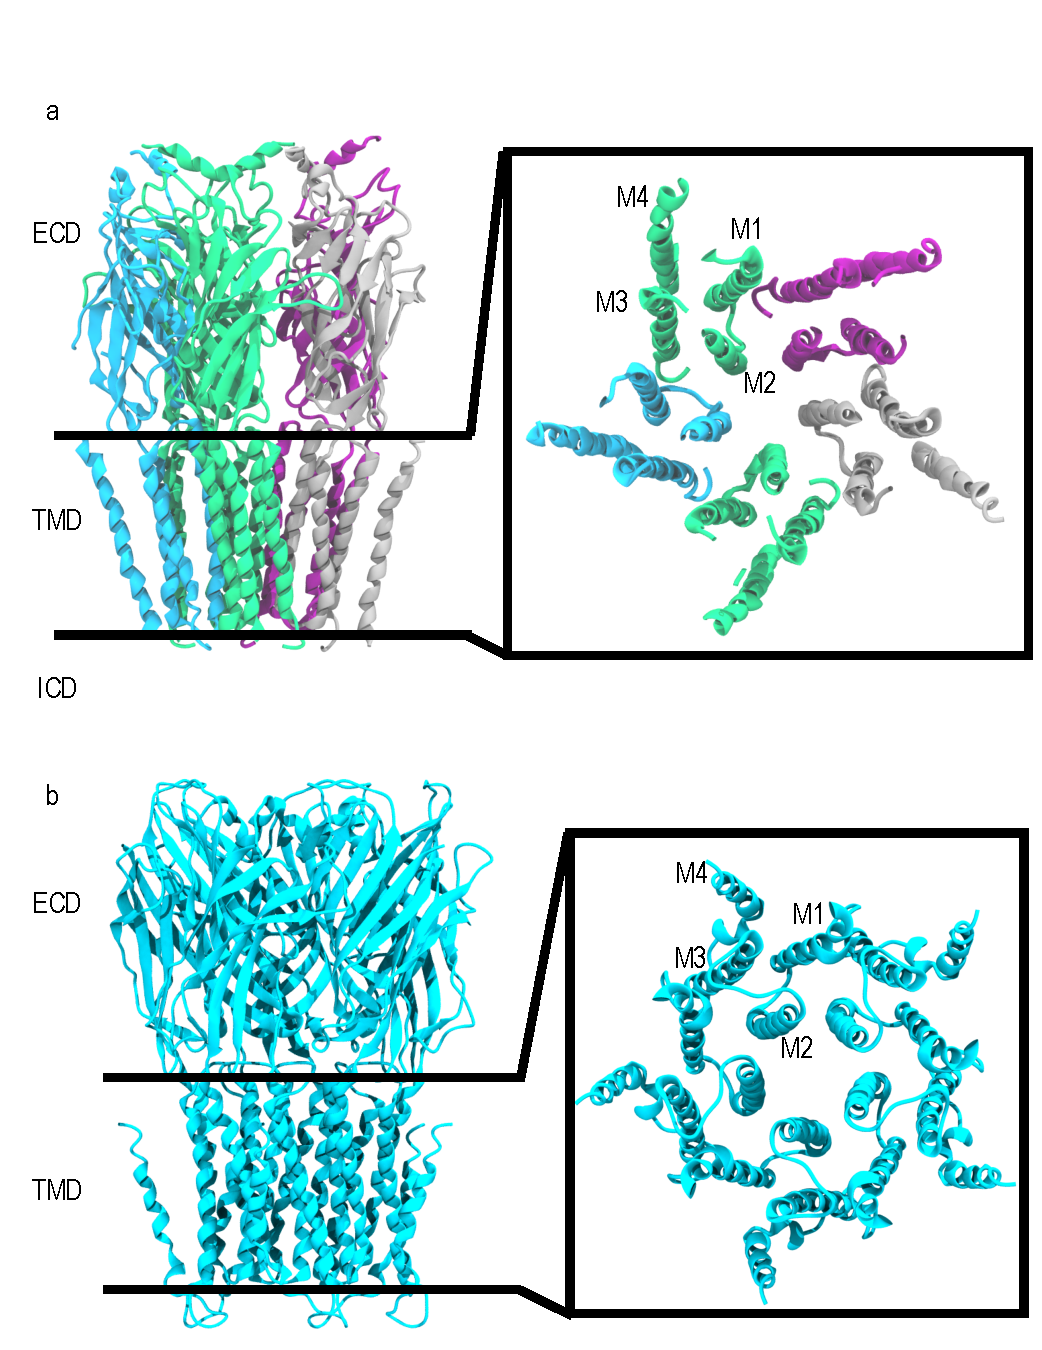
\includegraphics[width=4in]{pLGIC_Struct.pdf}
	\begin{flushleft}

	\caption[Protein structure of the nicotinic acetylcholine receptor and Erwinia ligand-gated ion channel.]{Protein structure of the nicotinic acetylcholine receptor and Erwinia ligand-gated ion channel. Visualization of  the a) neuronal nicotinic acetylcholine receptor (\nachr) \citep{Unwin2005} and b) Erwinia ligand-gated ion channel (ELIC). Left: Structure shown from a side view. ECD is comprised of beta sheets. TMD are alpha helices. The ICD is disordered and not shown.  \nachr~colored: $\alpha$: green, $\gamma$: blue, $\delta$: grey, $\beta$: purple. ELIC colored in cyan. Right: The TMD looking down from the ECD.   M4 directly interact with lipids, and provide the conical/star shape. M1 and M3 make up a cylindrical ``body'' of the channel. M2 lies the central pore.}
	\end{flushleft}

	\label{fig:struct}
\end{figure}

\plgic~function is modulated by the membrane lipid composition \citep{Salari2014,Corradi2018,Cheng2018}. \plgic-lipid interactions have been studied for more than 40 years, however the modulatory mechanism remains unclear \citep{Epstein1978,SCHIEBLER1978,Dalziel1980,Sunshine1994,Chen2007,Sogaard2006,Salari2014,Laverty2017,Cordero-Morales2018}.  One of the most well studied \plgic s is \nachr. When \nachr s are reconstituted in model membranes (synthetic membranes of 1 to 3 lipids) a minimum of $10-20\%$ cholesterol is required to restore native function to the channel. Anionic phospholipids, with cholesterol,  have also been shown to stabilize \nachr~under very specific conditions \citep{Ellena1983,Fong1986,Fong1987,Jones1988,Sunshine1994,DaCosta2009b,Hamouda2006a,DaCosta2004}. Yet is is not known where these lipids bind, with what affinity, or how they affect channel conformation. %Model membranes are frequently used to determine what \plgic's boundary lipids are. 

\section{Lipids and Membranes}

Lipids are a wide class of small amphiphilic molecules used biologically as signaling molecules \citep{Guesnet2011,Sezgin2012}, protein modulators \citep{Dacosta2013,Nemecz2016}, and essential component of membranes \cite{yeagle2016}. Two sub-lipid groupings are phospholipids and sterols  \citep{Burger2000,Simons2000,Shevchenko2010,buehler2016,yeagle2016}. Phospholipids are molecular structures consisting of a zwitterionic head groups, like phosphatidylcholine, or charged head groups, like phosphoserine, a glycerol- or sphingosine-back bone, and two fatty acid hydrocarbon chains (acyl-chains) which vary in both length and saturation. Saturated acyl-chains, such as the medium length palmitic acid(C16:0), add order to the overall membrane. Unsaturated  acyl-chains  decrease overall membrane order and increase membrane permeability. Unsaturated acyl-chains can be monounsaturated (a single kick cause by a double bond) like Oleic acid (18:1), or polyunsaturated (multiple kinks caused by multiple double bonds). The quintessential polyunsaturated fatty acid (PUFA) is the n-3 PUFA docosahexaenoic acid (C22:6) (DHA). DHA plays a number of roles in membrane organization \citep{Stillwell2003a,Gawrisch2003}, and neurological disorders \citep{Guesnet2011,DeFelice2012,Manor2011,McNamara2008}.

Sterols are a group of small rigid molecules with small neutral head groups and short rigid tails. Sterols are found throughout bacteria (hopanoids) \citep{Ourisson1992}, plants (phytosterols) \citep{Mlayeh2010}, fungi (ergosterol)\citep{Schneiter1999}, and animals (cholesterol). Cholesterol is essential to hormone synthesis and signaling \cite{buehler2016}. In membranes, it decreases membrane permeability and the average area per lipid and adds order to the bulk membrane \citep{YeagleCH9}. Cholesterol is also an essential lipid to restore function to \nachr~when reconstituted into model membranes.  

Model membranes often contain cholesterol, saturated, and monounsaturated lipids, with neutral or anionic head groups. Synthesizing model membranes with cholesterol and homo-acidic saturated and unsaturated lipids can result in lipid domain formation. Domain formation is the de-mixing of ordered saturated lipids and cholesterol from less ordered unsaturated lipids, forming liquid ordered ($\lo$) and liquid disordered ($\ldo$) domains respectively\citep{Kaiser2009,Lingwood2010}, see Figure \ref{fig:domain}. Domain formation, which requires spatial separation of saturated and unsaturated chains, is possible for mixtures of homo-acidic lipids, but not for hetero-acidic lipids containing both a saturated and unsaturated chain.  Hetero-acidic lipids are more common in native membranes \citep{Isolated1969, Breckenridge1973,Barrantes1989a,Taguchi2010,Quesada2016,Ingolfsson2017b,Lorent2020}, so it is likely that well-defined domains are less common in such membranes. Model membranes are useful tools for developing predictive models, but they lack the lipid diversity and the physical traits of realistic membranes.

%Ideally if a \plgic~is found in either domain it is reasonable to assume the \plgic's boundary lipids will be the same as the domain's lipids. This is not always the case. \cite{Bermdez_Partition_2010} suggested \nachr resided the $\lo$ and $\ldo$ interface. %However, using non-domain forming lipids we predicted polyunsaturated fatty acids (PUFA), cholesterol and saturated lipids sites around \nachr \cite{Woods2019}.  

The native membrane of model organisms such as \xo may have more than thirty phospholipid species \citep{Gamba2005,Ferreira2010} compared to the handful in model membranes. \plgic~native membranes, such as neuronal membranes or \textit{Torpedo} electric organs have more than 30 species of phospholipid \citep{Isolated1969, Taguchi2010, Breckenridge1973,Ingolfsson2017b,Barrantes1989a,Quesada2016}. When \nachr~is studied in \textit{Xenopus} oocytes, its current is reduced from native values but can be restored with lipid additives, such as asolectin \citep{Regost2003} to conduct ions. This suggests lipid diversity is not sufficient for native function, and that there are specific lipids required for \nachr~function not found in \xo or (not enough of these specific lipids to play a boundary role). 
\begin{figure}[!h]
\center
	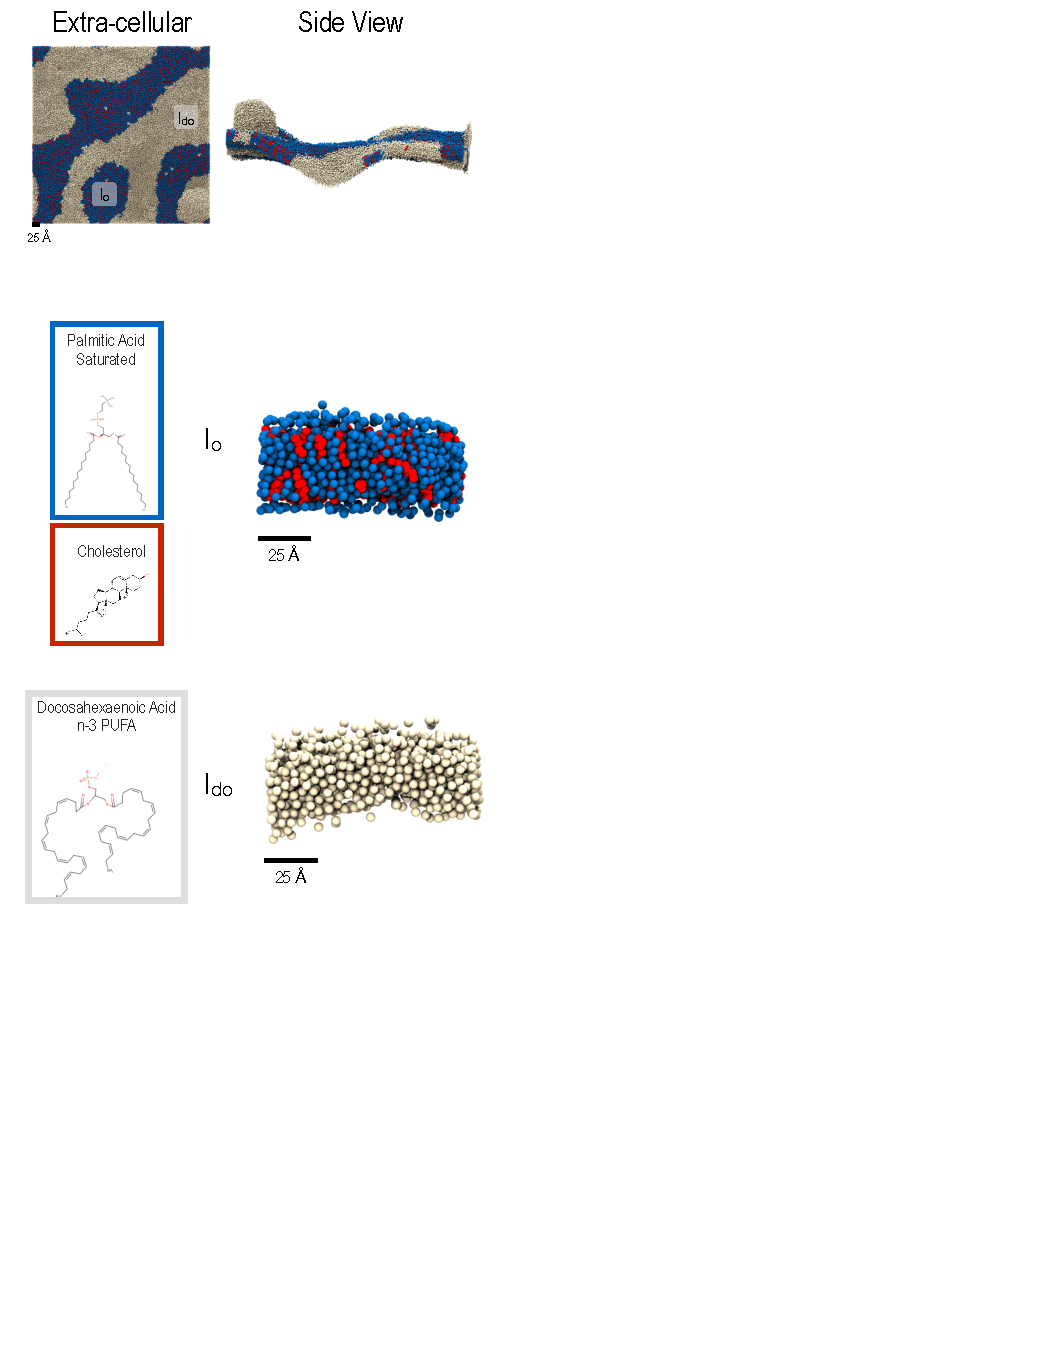
\includegraphics[width=3in]{Domains.pdf}
	\begin{flushleft}

	\caption[Domain formation in model PUFA rich domain forming membranes.] {Domain formation in model PUFA rich domain forming membranes Membranes are 75x75 nm$^2$ of 40:40:20 of n-3 PUFA:saturated:cholesterol, cream, blue, and white respectively. Row one shows the membrane from the extra-cellular domain and a side view. Row two shows a segment of a $\lo$ domain. Row three shows a segment of a $\ldo$ domain.}
	\end{flushleft}

	\label{fig:domain}
\end{figure}

\section{Boundary Lipids}

Boundary lipids are lipids in direct contact with a protein's TMD.  In random mixtures, the boundary lipid distribution would reflect the bulk distribution, but there is significant evidence that specific binding of lipids plays a key role in channel function. The most well studied \plgic, \nachr, ~is functionally dependent on cholesterol and anionic lipids \citep{Dalziel1980,Ellena1983,M.CriadoH.Eibl1982,Fong1986,Fong1987,Jones1988a,Sunshine1994,DaCosta2009b}, and many of these studies have demonstrated a role for direct interactions. Yet the precise location of lipid binding sites for \plgic s are still relatively unknown. Structural biology has detected cholesterol and fatty acid binding sites in \plgic s \citep{Addona1998,Althoff2014,Laverty2017,Basak2017,Henault2019}. Brannigan et al 2008 \cite{Brannigan2008} demonstrate cholesterol embedded within \nachr~ helped stabilize the protein's structure. Similarly Cheng et al 2009 \cite{Cheng2009} showed both cholesterol and anionic lipids with small head groups like phosphatidic acid (PA) could bind non-annularly to neuronal $\alpha$4$\beta$2 nAChR, and the anionic head group stabilizes the ECD during gating. %\cite{Henault2019} show by mutagenesis removed predicted lipid binding sites from ELIC resulting in a drop in channel current.

The M4 alpha helices have been shown to play a role in lipid sensing \citep{Henault2015}.  Basak et al \cite{Basak2017} found DHA bound around the M4 region in GLIC. DHA is a highly flexible PUFA, and if it binds to M4 it may play a role in minimizing membrane deformation caused by M4.

% Structural biology has found potential cholesterol sites at the subunit interface \citep{Laverty2017, Budelier2019}, potential specific phospholipid sites in the inter-subunit site \citep{Basak2017,Henault2019}, and inter-subunit sites sites \citep{Kim2020}. Molecular dynamics (MD) simulations predicted non-annular cholesterol site in \nachr~\citep{Brannigan2008}, cholesterol and anionic phospholipids favorably interacted with  \gabaa~over neutral phospholipid \citep{Cheng2009} and inter-subunit cholesterol sites in \gabaa~\citep{Hnin_A_2014}. 

\plgic s are structurally similar and it is likely that the distribution of acyl-chains and cholesterol is related across \plgic~sequences. Differences in \plgic~sequences may result in variation of charged lipid distribution. \nachr~and \gabaa~\\have positive amino acids in the lower portion of their M4 alpha helices, while ELIC has positive amino acids at inter-subunit sites, see Figures \ref{fig:aaa}. When boundary lipid requirements are not met, either by a complete absence or too few necessary lipid species, it is likely \plgic s will not maintain native current. 

%but sequentially different. While charged lipid may bind to different sites across the \plgic~family, .  Distribution of specific lipids may be critical to function and when a protein is reconstituted or grown in a non-native membrane it either lacks essential lipids or is in competition with other proteins for essential lipids, inpovereshes function.

%Hypothesized essential boundary lipids are cholesterol and n-3 polyunsaturated fatty acids (PUFAs). Cholesterol makes up $\sim40\%$ of the neuronal membrane and only $\sim20\%$ in \textit{Xenopus} oocytes. n-3 PUFAs compose $\sim15-20\%$ of phospholipids found in \plgic native membranes, but only $\leq10\%$ in \textit{Xenopus} oocyte. Cholesterol and n-3 PUFAs play complementary rolls in membranes. Cholesterol decreases membrane permeability and the average area per lipid, and adds order to the bulk membrane \citep{YeagleCH9}. n-3 PUFAs increases membrane permeability and decreases order in a membrane \cite{Stillwell2003a,Gawrisch2003}. However, both cholesterol and n-3 PUFAs assist in domain formation. 
%
%Occupation of \plgic s by specific boundary lipid appears to be driven by the \plgic's structure and and sequence. The M4 alpha-helices have the highest probability to interact with unsaturated lipids and cholesterol. We hypothesize that polyunsaturated fatty acids (PUFA) minimize the membrane deformation caused by the conical-star shape M4 alpha-helices provide, see Figure \ref{fig:struct}, and cholesterol helps stabilize the structure. Inter-subunit sites have the highest probability to interact with saturated lipids, n-3 PUFAs, and cholesterol. We hypothesize n-3 PUFAs and cholesterol stabilize the protein's structure, and saturated lipid's low flexibility fit interact favorably with \plgic's cylindrical inter-subunit sites. The sequence of the \plgic's structure dictates the location of anionic lipid binding. The prokaryotic \plgic~ELIC's inner inter-subunit sites tend to be occupied by anionic lipids, however \nachr's inner M4 sites tend to be occupied by anionic lipids. As such, the acyl-chain distribution of lipids does not appear to change significantly between \plgic s, but occupancy of head group charge various by protein sequence, see Figures \ref{fig:ELICGABA}a and \ref{fig:fig2} for domain partitioning, and Figures \ref{fig:aaa}b and \ref{fig:ELICGABA}b charged amino acids. 

\section{Approaches to Determining \plgic~Boundary Lipids}

It is experimentally challenging to capture the boundary lipid composition and and distribution for membrane channels. By nature lipids are small fluid molecules. Structural biology techniques such as cryogenic electron microscopy (cryo-EM) and X-ray crystallography can demonstrate where lipids are binding \citep{Kumar2019,Henault2019} but not the probability of lipid binding. Furthermore, determining which lipids have bound can be challenging as cryo-EM and x-ray crystallography require frozen or ``solid'' structures to image. Due to lipid's fluid nature and multiple conformations, lipids introduce significant crystallographic disorder, which prevents identification lipid of species. 

Mass spectrometry (MS) can be used to determine boundary lipid composition, including how many of a specific lipid reside around a protein. MS is not an imaging technique and can not provide protein structure or conformation information. Like cryo-EM and x-ray crystallography, MS cannot provide functional information \citep{Lorenzen2010}. 
 
Functional experiments, such as electrophysiology and fluorescence quenching, can predict lipid modulated function by varying the membrane lipid concentration \citep{Criado1984}. However functional experiments cannot directly show if the lipids used affect the protein from the bulk, or from specific region of the protein. Mutagenesis may provide indirect information but is not straightforward to interpret.

MD simulations are an optimal approach to predicting protein boundary lipids. MD is inherently fluid with molecular resolution. Using crystal and cryo-EM structures embedded in membranes based on model or realistic membrane compositions, MD simulations can be used to visualize lipids occupying potential binding sites. Furthermore the ability to visualize protein-lipid interaction allows straight forward prediction of the interactions driving lipid binding. While not necessarily useful for predicting how lipids modulate protein function, MD can be run using open, closed, and desensitized states of channel proteins to track changes in the structural role lipids play. 

MD comes in multiple forms, though two of the most widely used are all atomistic (AA) and coarse grained (CG). AAMD, modeled using all the atoms in a molecule, is limited by the molecular complexity, system size, and a time step on the $\sim 2$ fs scale. Tracking lipid diffusion from the bulk to the protein is computationally expensive and not always a viable approach. CGMD reduces the resolution of a molecule, for instance, the MARTINI forcefield \citep{Marrink2007} combines $\sim4$ atoms into a single bead. The reduced resolution allows for complex and large scale molecular systems at relatively larger time step ($\sim10$ fs scale), allowing lipids to diffuse from the bulk to a channel and back. This makes CGMD a powerful technique for predicting boundary lipids, membrane deformation, and protein-protein interactions within a membrane.

\section{Goals of this Thesis}

This thesis aims to identify specific lipid binding sites on pLGICs, as well as the effect of lipid topology and bulk membrane composition on occupancy of these sites. CGMD has been used for various small proteins in model to realistic membranes \citep{Hung2011,Domanski2012,Parton2013,Flinner2015,Lin2018} but \plgic s had solely been simulated using AAMD in model membranes lacking many essential native lipids. AAMD simulations provide critical predictions of how lipids bind to specific sites around \plgic s and can predict how lipid are structurally important to proteins. CGMD allows complex lipid compositions to diffuse around one or more \plgic s and equilibrate to the most likely 1) boundary composition and 2) lipid distribution. Over four chapters, I will quantify the boundary lipids of pLGICs in a series of increasingly complex membranes, beginning with a simple model membrane and culminating in a quasi-native neuronal membrane.   

%Chapter 2 uses the n-6 and n-3 PUFAs Linolic acid (LA) and DHA, both prominent PUFAs in \textit{Torpedo}'s electric organ \citep{Barrantes1989a,Quesada2016} in two series of model ternary membranes consisting of one PUFA, palmitic acid, and cholesterol. A single neuromuscular \nachr \citep{Unwin2005} is embedded in both series of membranes to determine if \nachr resides in a $\lo$ or $\ldo$ domain and what are \nachr's boundary lipid. As of the publication of chapter 1, it was the first CGMD simulation to use a \plgic~in association with a n-3 PUFA.
%
%Chapters 3 and 4 focus on boundary lipid distributions. The work from chapter 2 is expanded on in chapter 3, using model ternary membranes of domain and non-domain forming DHA, palmitic acid, and cholesterol with one to four neuromuscular \nachr s \citep{Unwin2005} embedded in each membrane. The domain forming and non-domain forming series are used to predict 1) \nachr-\nachr~clustering between domain and non-domain forming membranes. 2) Determine the difference in boundary lipid acyl-chain distributions in domain and non-domain forming membranes. Chapter 4 uses model binary systems consisting of 1-palmitoyl-2-oleoyl-sn-glycero-3-phosphocholine (POPC) and 1-palmitoyl-2-oleoyl-sn-glycero-3-phosphoglycerol (POPG) or 1-palmitoyl-2-oleoyl-sn-glycero-3-phosphoethanolamine (POPE) and POPG with ELIC \citep{Pan2012} embedded in both series. Enrichment and polar density plots are used to determine whether neutral or anionic lipids are more favorable in ELIC's boundary lipid composition, and how anionic lipids are distributed.

%Chapter 5 unifies the elements of the previous chapters. 
Chapter 2 demonstrates neuromuscular \nachr-lipid \citep{Unwin2005} interaction in model PUFA rich domain forming membranes. I examine  protein-membrane domain partitioning, boundary lipid distributions and present a potential explanation for PUFA- and cholesterol-\nachr~interactions. Chapters 3 and 4 predict specific lipid occupancy sites around the TMD for lipid acyl-chain saturation and head group charge. Chapter 3 expands on the work of chapter 2, comparing \nachr~boundary lipid distributions in PUFA rich model membranes with and without domain formation. Chapter 4 does not consider PUFAs and focuses on the distribution of anionic lipids around ELIC \citep{Pan2012} embedded in binary non-domain forming membranes. Chapter 5 unifies the elements of the previous chapters. Unlike the previous model membranes, we use a quasi-neuronal membrane of 36 different lipid species with both neutral and anionic head groups \citep{Ingolfsson2017b}. We determine boundary lipid distributions for \nachr, quantify specific binding using a new affinity calculation method, and compare to  results from model membranes in chapters 2 to 4.

%Predicting boundary \plgic boundary lipid and specific sites of protein occupancy has been exhaustedly done in model computational membranes. These model membranes have provided invaluable predictive models, however \plgic~native boundary lipids are unknown. This thesis is the accumulation for four projects working to predict \plgic~boundary lipids in coarse-grained model and quasi-realistic membranes. Chapter 1 looks at where \nachr~resides in domain forming membranes. Chapter 2 compares domain and non-domain forming membranes for multiple \nachr~and predicts locations for lipid occupancy. Chapter 3 is computational work from a collaborative project, predicting anionic occupancy sites for the \plgic~ELIC. Chapter 4 embeds \nachr~in a quasi-native membrane, and tests the predicted occupancy sites from chapters 2 and 3 by calculating the binding affinity of acyl-chain saturation and head group charge.

\chapter{Boundary lipids of the nicotinic acetylcholine receptor: spontaneous partitioning via coarse-grained molecular dynamics simulation}
Originally published in: Biochimica et Biophysica Acta - Biomembranes, 2019, vol. 1861, issue 4, pages 887-896\\ \\
%\setcounter{savepage}{\thepage}
{Liam Sharp$^1$}  {Reza Salari$^{1,2}$} {Grace Brannigan$^{1,3}$}
{1) Center for Computational and Integrative Biology, Rutgers University-Camden, Camden, NJ} {2) Now at Washington University School of Medicine in St Louis} {3) Department of Physics, Rutgers University-Camden, Camden, NJ}
\section{Abstract}
Reconstituted nicotinic acetylcholine receptors (nAChRs) exhibit significant gain-of-function upon addition of cholesterol to reconstitution mixtures, and cholesterol affects organization of nAChRs within domain-forming membranes, but whether nAChR partitions to cholesterol-rich liquid-ordered (``raft'' or $\lo$) domains or cholesterol-poor liquid-disordered ($\ldo$) domains is unknown. We use coarse-grained molecular dynamics simulations to observe spontaneous interactions of cholesterol, saturated lipids, and polyunsaturated (PUFA) lipids with nAChRs. In binary Dipalmitoylphosphatidylcholine:Cholesterol (DPPC:CHOL) mixtures, both CHOL and DPPC acyl chains were observed spontaneously entering deep ``non-annular'' cavities in the nAChR TMD, particularly at the subunit interface and the $\beta$ subunit center, facilitated by the low amino acid density in the cryo-EM structure of nAChR in a native membrane. Cholesterol was highly enriched in the annulus around the TMD, but this effect extended over (at most) 5-10\AA. In domain-forming ternary mixtures containing PUFAs, the presence of a single receptor did not significantly affect the likelihood of domain formation.  nAChR partitioned to any cholesterol-poor $\ldo$ domain that was present, regardless of whether the $\ldo$ or $\lo$ domain lipids had PC or PE headgroups. Enrichment of PUFAs among boundary lipids was positively correlated with their propensity for demixing from cholesterol-rich phases. Long $n - 3$ chains (tested here with Docosahexaenoic Acid, DHA) were highly enriched in annular and non-annular embedded sites, partially displacing cholesterol and completely displacing DPPC, and occupying sites even deeper within the bundle. Shorter $n - 6$ chains were far less effective at displacing cholesterol from non-annular sites.
%\end{abstract}
%\setcounter{page}{\thesavepage}
%\stepcounter{page}

\section{Introduction}
\label{S:1}

The nicotinic acetylcholine receptor (nAChR) is an excitatory pentameric ligand gated ion channel (pLGIC) commonly found in the neuronal post synaptic membrane and neuromuscular junction (NMJ) in mammals 
as well as the electric organs of the \textit{Torpedo} electric ray. 
nAChRs play a fundamental role in rapid excitation within the central and peripheral nervous system, and neuronal nAChRs are also critical for cognition and memory \citep{Dani2001b, Changeux2015}. Acetylcholine is the orthosteric \nachr~ligand, but numerous other exogenous and endogenous small molecules modulate \nachr s, including nicotine, general anesthetics, the tipped-arrow poison curare,  phospholipids, cholesterol, and cholesterol-derived hormones.\citep{Klaassen2015,Taly2009}  
The larger pLGIC super family that includes \nachr s has been shown to play roles in numerous diseases related to inflammation, \citep{Patel2017,Yocum2017,Cornelison2016}, addiction \citep{Cornelison2016}, chronic pain \citep{Xiong2012}, Alzheimer's Disease \citep{Walstab2010,Picciotto_Neuroprotection_2008,MartinRuiz_4_1999}, spinal muscular atrophy \citep{Arnold_Reduced_2004}, schizophrenia \citep{Haydar2010} and neurological autoimmune diseases \citep{Lennon_Immunization_2003}.

nAChRs are highly sensitive to the surrounding lipid environment\citep{Hamouda2006a,Baenziger2017,Padilla-Morales2016,Barrantes2007} for reasons that remain poorly understood. In the late 1970s it was observed that reconstituted \nachr s only exhibit native conductance if model phospholipid membranes contained at least 10-20\% cholesterol
\citep{Dalziel1980,Criado1982,Ochoa1983}. Three generations of investigation into the mechanism have followed, with the first generation of studies\citep{Marsh1978,Dalziel1980,Marsh1981,Criado1982,Gonzalez-Ros1982,McNamee1982,Ellena1983,Ochoa1983,Zabrecky1985,Bristow1987,Leibel1987,Middlemas1987,Jones1988a,Jones1988, Fong1986,McNamee1988, Barrantes1989a,Sunshine1992,Sunshine1994,Narayanaswami1993,Addona1998,Corbin1998,Barrantes2000} aiming to differentiate between the role of bulk, annular, and non-annular cholesterol. The second generation\citep{Baenziger2015,Bruses2001,Marchand2002,Oshikawa2003,Pato2008,Zhu2006a,Baenziger2017, Barrantes2007,Barrantes2000,Barrantes2010,Bermudez2010,Perillo2016,Wenz2005,Borroni2016, Unwin2017} of studies probed membrane-mediated effects on organization of multiple \nachr s, while the third generation\citep{Basak2017,Althoff2014,Laverty2017,Zhu2018} has applied x-ray crystallography and high-resolution cryo electron microscopy to directly observe lipid binding modes. 

Members of the pLGIC family other than \nachr~are also lipid-sensitive,\citep{Dunn1989,Sooksawate2001,Baenziger2011, Dostalova2014} and lipids other than cholesterol can also modulate function\citep{Bhushan1993,Cheng2007,Corrie2002,Corrie2002,Rankin1997,Wenz2005,Hamouda2006a}, but these mechanisms have not been as extensively studied.  The recent publication of several crystal and cryo-EM structures \citep{Basak2017,Althoff2014,Laverty2017,Zhu2018}
has confirmed that specific lipid-pLGIC interactions extend beyond cholesterol and \nachr.  Such interactions are also well-established in other transmembrane proteins, including G-protein coupled receptors (GPCRs) and other ion channels, as reviewed in \citep{Burger2000, Lee2004, Pucadyil2006a, Landreh2016, Smithers2012}. 

Even in the specific case of cholesterol-\nachr~ interactions, results from different approaches have suggested complex behavior and even contradictory interpretations.  Results have indicated that both cholesterol enrichment\citep{Dalziel1980,Criado1982,Ochoa1983} and cholesterol depletion\citep{Santiago2001} cause gain of function, that anionic phospholipids are unnecessary for native function\citep{Dalziel1980,Criado1982,Ochoa1983} or must be\citep{Corrie2002,Corrie_Lipid_2002} included in a reconstitution mixture,  that cholesterol increases \nachr~clustering\citep{Pato2008, Zhu2006a, Barrantes2007} and directly interacts with \nachr~\citep{Leibel1987,Jones1988}, but \nachr~does not consistently partition into cholesterol-rich domains\citep{Bermdez_Partition_2010}. We suggest here that some of these apparent contradictions may be explained by competition between cholesterol and other lipids found in native membranes, primarily lipids with polyunsaturated fatty acyl chains (PUFAs).   

Interactions of \nachr~ with PUFAs have not been systematically investigated experimentally, but a large amount of circumstantial experimental evidence suggests an important role for PUFAs in \nachr~ function.    Clinically, long-chain $n-3$  (commonly called ``Omega-3'' or $\omega-3$) lipids have a neuroprotective role\citep{Piomelli2007}, and \nachr-associated pathologies can arise for patients with low levels of $n-3$ PUFAs. $\alpha7$ \nachr s are implicated in schizophrenia\citep{Haydar2010}, and dietary supplementation with $n-3$ fatty acids (usually through fish oil) can reduce the likelihood of psychosis, with dramatic effects in some individual cases\citep{Amminger2010}.

{\it In vitro}, PUFA-rich asolectin\citep{Regost2003,Olsen2003} is one of the most robust additives\citep{Criado1982} for obtaining native \nachr~function: restoration of native function by cholesteryl hemisuccinate (CHS) is observed only over a narrow CHS concentration range in monounsaturated PE/PS membranes, but a much wider concentration range in asolectin\citep{Criado1982}. The specific component(s) of asolectin that complement cholesterol in improving \nachr~function have not been isolated. 
Long chained $n-3$  
PUFA lipids are abundant in two seemingly disparate \nachr~native membranes: mammalian neuronal membranes\citep{Breckenridge_Adult_1973,Isolated1969} and those of the \textit{Torpedo} electric organ,\citep{Barrantes1989a,Quesada2016}. Both such membranes also have an abundance of phosphoethanolamine (PE) headgroups and saturated glycerophospholipids, and a scarcity of monounsaturated acyl chains and sphingomyelin compared to thhe \textit{Xenopus} oocyte membranes \citep{Gamba2005} common in functional studies, or a ``generalized'' mammalian cell membrane \citep{Ingolfsson2014}.    

Membranes composed of ternary mixtures of saturated lipids, unsaturated lipids, and cholesterol tend to demix into separate domains. Saturated lipids and cholesterol constitute a rigid liquid ordered phase ($\lo$) in which acyl chains remain relatively straight. \citep{Feller_Acyl_2008,Yeagle2016115,Cicuta1981,Bleecker2016} Unsaturated lipids form a more flexible liquid disordered phase ($\ldo$) in which the chains remain fully melted.  
$\lo$ domains are often visualized as signaling ``platforms'', restricting membrane proteins into high density ``rafts'' that diffuse within a fluid membrane {\citep{Simons1997,Simons2000}}. This conceptualization requires that $\lo$ domains have a much smaller area than $\ldo$ domains, and does not well-represent membranes that are over 30\% cholesterol, such as neuronal membranes.   

The first generation of studies into the mechanism underlying cholesterol-modulation of \nachr~ were conducted and interpreted in an era preceding the discovery of lipid-induced domain formation in membranes. 
The second generation explicitly considered potential interactions of \nachr~with lipid domains, in part to determine the requirements for the extremely high density  ($\sim10^{4}\mu^{-2}$) of \nachr s at the neuromuscular junction \citep{Breckenridge1972}.  Since direct interaction between \nachr~and cholesterol had been demonstrated in the first generation of studies, a sensible initial hypothesis was that \nachr~persistently partitioned to $\lo$ domains, retaining little contact with unsaturated chains.  Tests of this hypothesis have yielded results that are inconclusive, contradictory, or highly sensitive to lipid composition.     

Barrantes and colleagues\citep{Wenz2005} found that the addition of \nachr s~to a domain-forming lipid mixture increased the size of Dipalmitoylphosphatidylcholine/Cholesterol (DPPC/Chol) lipid-ordered domains, which (combined with additional FRET data) was interpreted as indicating \nachr~was embedded in liquid-ordered domains.  Some studies \citep{Marchand2002,Stetzkowski-Marden2006,Willmann2006} suggest that \nachr s are associated with microdomains independently of stimulation by other proteins associated with the neuromuscular junction. Other studies\citep{Zhu2006a,Campagna2006} suggested that \nachr s require stimulation by a protein such as agrin to partition into microdomains. Formation and disassembly of the \nachr-rich microdomains is highly sensitive to cholesterol concentration.\citep{Barrantes2007,Bruses2001,Marchand2002,Zhu2006a,Pun2002}

These studies suggested a role for cholesterol-induced phase separation, but did not confirm that \nachr~partitions to the cholesterol-rich phase.  To test for an intrinsic \nachr~ domain preference, Barrantes and co-workers checked for enrichment of \nachr s in the detergent resistant membrane (DRM).   \nachr s were not enriched in the DRM of a model, domain-forming mixture (1:1:1  Chol: palmitoyloleoylphosphatidylcholine(POPC): sphingomyelin) \citep{Bermdez_Partition_2010} but inducing compositional asymmetry across leaflets did yield \nachr~enrichment in the DRM fraction \citep{Perillo2016}.  While more precise and robust experimental methods for determining partitioning preference and specific boundary lipids such as mass spectrometry have been applied for other transmembrane proteins\citep{Gupta2018,Chorev2018}, they have not been applied to complex heteromers like \nachr.  

Fully atomistic molecular dynamics (MD) simulations\citep{Brannigan2008, Cheng2009, Hnin_A_2014, Carswell_Role_2015} have served as a natural complement to the third-generation structural biology approach, but are limited in their ability to resolve contradictions between first and second generation studies, because lipids are unable to diffuse over simulation time scales.\citep{Ingolfsson2014,Bond2006,Parton2013,Goose2013,Scott2008}.   Efficient lipid diffusion is a requirement for equilibrating domains or detecting protein-induced lipid sorting.    Coarse-grained MD (CG-MD) has been used to great success in a number of simulations for both lipid-protein binding and membrane organization \citep{Bond2006,Scott2008,Parton2013,Goose2013,Iyer2018,Sodt2014}. Here we use CG-MD as a ``computational microscope'' to observe the equilibrium distribution of lipids local to the \nachr~ in a range of binary and ternary lipid mixtures inspired by native membranes.   We observe a remarkable enrichment of polyunsaturated lipids among \nachr~boundary lipids. To our knowledge, these are the first molecular simulations of the \nachr~in non-randomly mixed membranes, and the first study to systematically investigate the likelihood of polyunsaturated lipids as \nachr~boundary lipids.  

\section{Methods}
\label{S:2}

\subsection{System Composition}

All simulations reported here used the coarse-grained MARTINI 2.2\citep{martini} topology and forcefield.
~nAChR coordinates were based on a cryo-EM structure of the $\alpha{\beta}\gamma\delta$ muscle-type receptor in native torpedo membrane (PDB 2BG9\citep{Unwin2005}). This is a medium resolution structure (4\AA) and was further coarse-grained using the martinize.py script; medium resolution is sufficient for use in coarse-grained simulation, and the native lipid environment of the proteins used to construct 2BG9 is critical for the present study. The secondary, tertiary and quaternary structure in 2BG9 was preserved via soft backbone restraints during simulation as described below, so any inaccuracies in local residue-residue interactions would not cause instability in the global conformation.  

Coarse-grained membranes were built using the Martini script insane.py, which was also used to embed the coarse-grained \nachr~within the membrane. The insane.py script randomly places lipids throughout the inter- and extra-cellular leaflets, and each simulation presented in this manuscript was built separately.  Binary mixed membranes were composed of one saturated lipid species (Dipalmitoylphosphatidylcholine (DPPC) or Dipalmitoylphosphatidylethanolamine (DPPE)) and cholesterol (CHOL), while ternary mixed membranes also included either two $n-6$ PUFA acyl chains : Dilinoleoylphosphatidylcholine (dLA-PC) or Dilinoleoylphosphatidylethanolamine (dLA-PE) or two $n-3$ PUFA acyl chains : \seqsplit{Didocosahexaenoylphosphatidylethanolamine} (dDHA-PE) or Didocosahexaenoylphosphatidylcholine (dDHA-PC). DHA-PC is not distributed with the MARTINI lipidome, but was constructed in-house using MARTINI DHA tails and PC headgroups). Multiple box sizes were used depending on the goal;  ``small'' boxes were between $22x22x20$ nm$^3$ and $25x25x25$ nm$^3$, with about {$\sim$ 1400} total lipids and {$\sim$ 80000} total beads, and were used primarily to investigate composition trends, ``large'' boxes were about $45x45x40$ nm$^3$ with about {$\sim$ 8,300} total lipids and {$\sim$ 820,000} total beads, and were used primarily to investigate subunit specificity and long-range sorting, and ``very large'' boxes were $\sim$ 75x75x40~nm$^3$ with about {$\sim$ 19,000} total lipids and {$\sim$ 1.8 million} total beads, and were used to verify that partitioning in the $\ldo$ phase did not reflect finite size effects.  


\subsection{Simulations}


Molecular dynamics simulations were carried out using GROMACS\citep{Berendsen1995}; small boxes used GROMACS 5.0.6 and large {and very large} boxes used  GROMACS 5.1.2 or 5.1.4. All systems were run using van der Waals (vdW) and Electrostatics in shifted form with a dielectric constant of $\epsilon_r$=15. vdW cutoff lengths were between 0.9 and 1.2 nm, with electrostatic cutoff length at 1.2 nm.

Energy minimization was performed over 10000 to 21000 steps.  Molecular dynamics were run using a time step of 25~fs, as recommended by MARTINI, for 2 $\mu$s for {small membranes,and 10 $\mu$s for large and very large membranes}. Simulations were conducted in the isothermal-isobaric (NPT) ensemble, by using a Berendsen thermostat set to 323 K with temperature coupling constant set to  1 ps, as well as isotropic pressure coupling with compressibility set to $3\times 10^{-5}$ bar$^{-1}$ and a pressure coupling constant set to 3.0 ps. 


Secondary structures restraints consistent with MARTINI recommendations were constructed by the martinize.py \citep{martini} script {and} imposed by Gromacs\citep{Berendsen1995}. Protein conformation was maintained in small systems via harmonic restraint (with a spring constant of 1000 kJ$\cdot$ mol$^{-1}$) on the position of backbone beads. \nachr~conformation in large systems was preserved via harmonic bonds between backbone beads separated by less than 0.5 nm, calculated using the ElNeDyn algorithm \citep{Periole_Combining_2009} associated with MARTINI\citep{martini}  with a coefficient of 900 kJ$\cdot$ mol$^{-1}$.  These restraints limited the root-mean-squared-displacement (RMSD) of the backbone to less than 2.5 \r{A} throughout the simulation.  

The minimum equilibration time depended on the system size. Small systems typically began domain formation by 500 ns, with domains fully formed by 1000 ns. Large systems and very large simulations required about 5$\mu$s of equilibration for stabilization of metrics described below.

\subsection{Analysis}

Extent of domain formation within the membrane was tracked by 
    \begin{equation}
    \begin{aligned}
      \m{A}{B} &\equiv \frac{\langle n_{A,B} \rangle} {6x_{B}} -1 \\
      \mself{A} &\equiv \frac{\langle n_{A,A} \rangle} {6x_{A}} -1 
    \end{aligned}
    \label{eq:M}
  \end{equation}
 where $n_{A,B}$ is the number of type B molecules among the 6 nearest neighbors for a given type A molecule,  the average is over time and all molecules of type $A$, and the self-association metric is notated $\mself{A} \equiv \m{A}{A}$ for brevity. For a random mixture, $\langle n_{A,B} \rangle = 6x_{B}$, where $x_{B}$ is the fraction of overall bulk lipids that are of type B. ${\mself{A}=0}$ indicates random mixing while ${\mself{A}>0}$  and ${\mself{A}<0}$ indicate demixing and excessive mixing respectively.  


Extent of receptor partitioning within the $\lo$ or $\ldo$ domain was tracked by counting the number $\bsat$ of saturated annular boundary lipids and comparing with the expectation for a random mixture, via the order parameter $\qsat$:
  \begin{equation}
    \begin{aligned}
      \qsat\equiv \frac{1}{\xsat}\left\langle\frac{  \bsat }{\nbound }\right\rangle-1,\\
    \end{aligned}
    \label{eq:Q}
  \end{equation}
  where $\nbound$ is the total number of lipids in the annular boundary region and $\xsat$ is the fraction of overall bulk lipids that are saturated phospholipids. $\qsat <0$ indicates depletion of saturated lipids among boundary lipids, as expected for partitioning into an $\ldo$ phase, while $\qsat>0$ indicates enrichment and likely partitioning into an $\lo$ phase. Each frame, $\nbound$ and $\bsat$ were calculated by counting the number of total and saturated lipids, respectively, for which the phosphate bead fell within a distance of 1.0~nm~ to 3.5~nm~ from the M2 helices, projected onto the membrane plane. 
  
  Two-dimensional density distribution of the beads within a given lipid species $B$ around the protein was calculated on a polar grid: 
  \begin{equation}
    \begin{aligned}
      \rho_{B}(r_i,\theta_j)= \frac{\left\langle n_{B}(r_i,\theta_j) \right\rangle}{r_i \Delta{r}\Delta{\theta}} \\        
    \end{aligned}
    \label{eq:R}
  \end{equation}
  where  $r_i = i \Delta{r}$ is the projected distance of the bin center from the protein center, $\theta_j = j \Delta{\theta}$ is the polar angle associated with bin j,  $\Delta{r}$= 10\AA~ and  $\Delta{\theta} = \frac{\pi}{15}$ radians are the bin widths in the radial and angular direction respectively, and $\left\langle n_{B}(r_i,\theta_j) \right\rangle$ is the time-averaged number of beads of lipid species $B$ found within the bin centered around radius $r_{i}$ and polar angle $\theta_{j}$.  In order to determine enrichment or depletion, the normalized density $ \tilde{\rho}_{B}(r_i,\theta_j)$ is calculated by dividing by the approximate expected density of beads of lipid type B in a random mixture, $x_{B}s_{B}~N_{L}/\langle L^{2}\rangle$, where $s_{B}$ is the number of beads in one lipid of species B, $N_{L}$ is the total number of lipids in the system, and $\langle L^{2}\rangle$ is the average projected box area: 
  \begin{equation}
    \begin{aligned}
  \tilde{\rho}_{B}(r_i,\theta_j)=\frac{ \rho_{B}(r_i,\theta_j)}{x_{B}s_{B}~N_{L}/\langle L^{2}\rangle} \\        
    \end{aligned}
    \label{eq:Rt}
  \end{equation}
  This expression is approximate because it does not correct for the protein footprint or any undulation-induced deviations of the membrane area.  The associated corrections are small compared to the membrane area and would shift the expected density for all species equally, without affecting the comparisons we perform here.   

 
\section{Results}
\label{S:3}
\begin{figure*}[h!]
	{
	\includegraphics[width=\linewidth]{ModelMemb_Images/DPPC_Only.pdf} }
	\caption[nAChR boundary lipids in binary mixtures of DPPC and CHOL.] {nAChR boundary lipids in binary mixtures of DPPC and CHOL. A: Representative frame from a simulated trajectory of a single nAChR embedded in a small membrane, colored by subunit ($\alpha$:green, $\beta$:purple, $\delta$:gray, $\gamma$:cyan) in a 4:1 DPPC (blue):Chol (red) mixture.  B: Extent of demixing ($\mself{DPPC}$ defined in Eq. \ref{eq:M}) and depletion of saturated lipids from the boundary ($\qsat$ defined in Eq.\ref{eq:Q}) in small binary membranes. In this binary system, cholesterol depletion/enrichment is directly related to the saturated lipid depletion/enrichment: $Q_\mathrm{chol}=-x_{\mathrm{sat}} \qsat/\xch$.  Error bars represent standard error for a blocking average over 50 ns. C: Average normalized density (Eq. \ref{eq:Rt}) of cholesterol for the system in A. Data is equivalent to that in Figure \ref{fig:sorting}: Binary Mixture ``Chol'' row.}%``Chol'' row, ``None'' column, but has been cropped and zoomed around the protein center.\grace{Update previous sentence upon inclusion of new figure}}
	\label{fig:binary}
\end{figure*} 
\subsubsection {Spontaneous association with cholesterol in binary membranes} \label{binary}

Lipid sorting was characterized for \nachr s in binary DPPC:CHOL membranes (Figure \ref{fig:binary}A)  using several metrics. 
Non-random lipid mixing (including domain formation) was quantified using the self-association metric $\mself{A}$ as defined in Equation \ref{eq:M}. 
As expected, in simulated binary membranes containing only DPPC and 0-40\% cholesterol, minimal demixing was observed, with values of $\mself{DPPC}$ (Fig \ref{fig:binary}B) rising slightly for higher cholesterol concentrations but remaining persistently below 0.05.  

Depletion of saturated lipids among \nachr~boundary lipids (relative to those expected for a random mixture) was quantified using the metric $\qsat$ defined in equation \ref{eq:Q}. Negative and positive values of $\qsat$ reflect depletion or enrichment of saturated lipids in the \nachr~boundary, respectively. In binary systems containing cholesterol and saturated lipids, depletion of saturated lipids corresponds directly to enrichment of cholesterol: $Q_{chol} = -\qsat x_\mathrm{sat}/\xch$. 

In binary DPPC:CHOL mixtures, $\qsat$ was very slightly negative for $\xch < 20\%$, but decreased steadily for higher concentrations. This trend indicates some depletion of DPPC (and enrichment of cholesterol) among \nachr~ boundary lipids (Figure \ref{fig:binary}B).  Typically, between 10 and 20\% cholesterol has been required in reconstitution mixtures to restore native function  \citep{Fong1986,Dalziel1980,Criado1982}  and a phase transition at about 20\% cholesterol in binary DPPC:CHOL model membranes is indicated by differential scanning calorimetry.\citep{Marsh2010} 

Spontaneous binding of cholesterol to non-annular or ``embedded'' sites, similar to what we previously proposed\citep{Brannigan2008}, was observed in these CG-simulations, and penetration of the TMD bundle by DPPC acyl chains was also observed at lower cholesterol concentrations (Fig \ref{fig:binary}A).  Distribution of density for embedded lipids is further discussed in Section 3.4.  

Annular cholesterol (enrichment of cholesterol at the protein-lipid interface), is visible for the binary systems via a ring of high (red) cholesterol density just around the protein in Figure \ref{fig:binary}C. Enrichment of cholesterol near the protein is highly localized with a ring that is less than 5\AA~wide. This is in general agreement with evidence for annular cholesterol in randomly-mixed binary membranes. \citep{Barrantes2010}




\subsection {Domains formed in PUFA-containing ternary membranes are not affected by introduction of an \nachr } \label{Demix}
	\begin{figure}[h!]
		{
		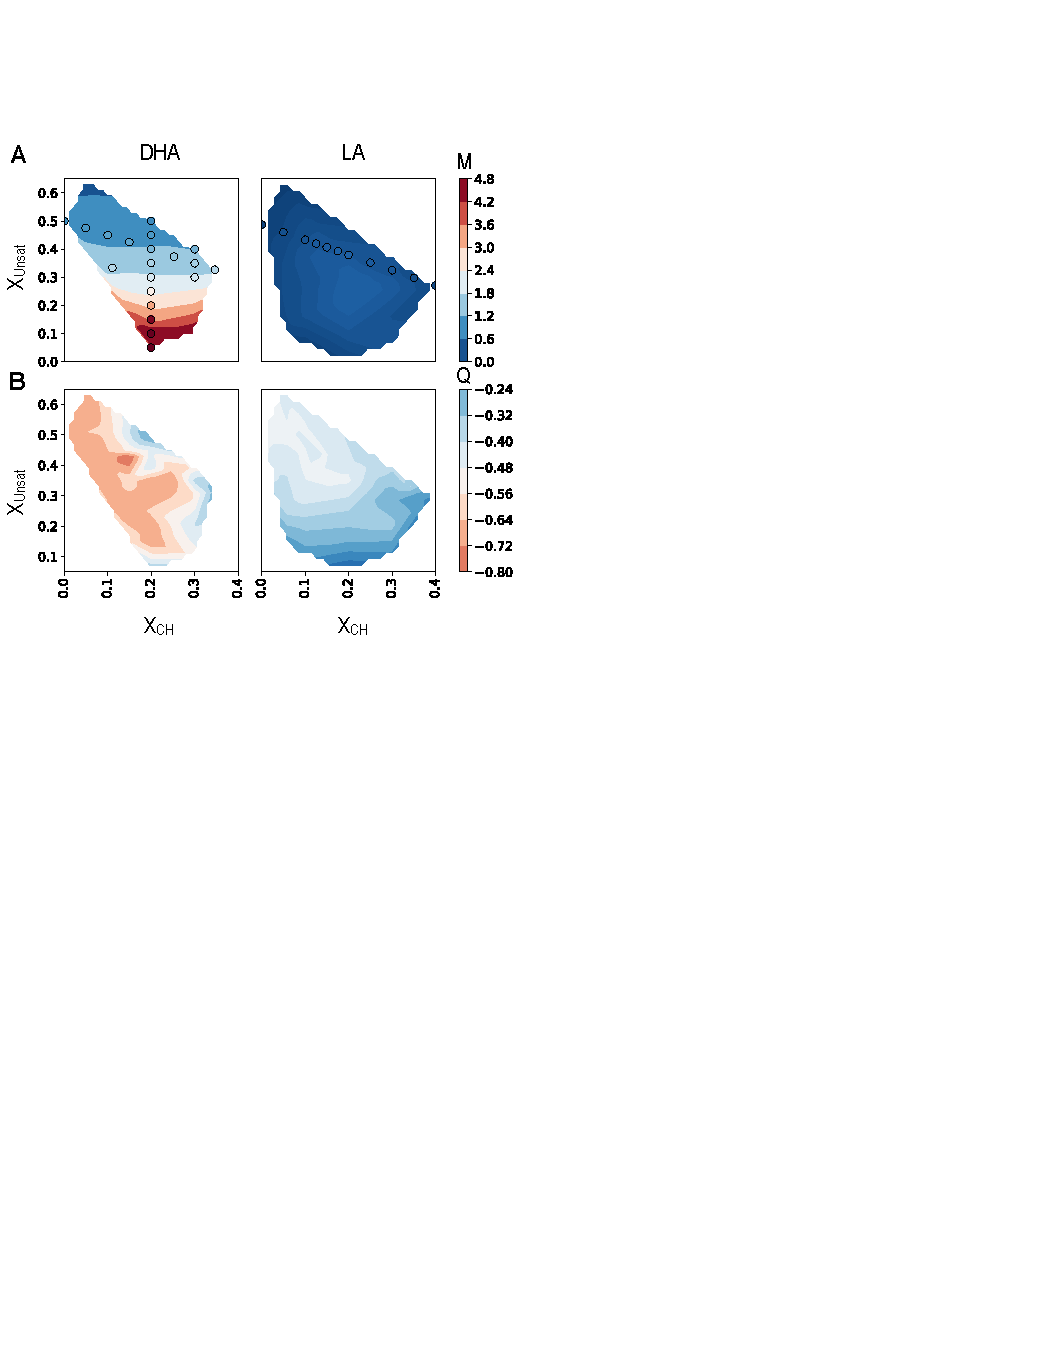
\includegraphics[width=1\linewidth]{ModelMemb_Images/Fig2.pdf}}
		\caption[Quantitative analysis of bulk membrane mixing and nAChR boundary lipid composition across small membranes containing DPPC, Cholesterol, and either dDHA-PE or dLA-PC.] {Quantitative analysis of bulk membrane mixing and nAChR boundary lipid composition across small membranes containing DPPC, Cholesterol, and either dDHA-PE or dLA-PC. Shaded contours were constructed based on 40 individual simulations with dDHA-PE and 30 with dLA-PC. A: $\mself{PUFA}$, defined in eq \ref{eq:M}.  Circles represent mixing of systems with the same lipid composition but no \nachr. B: $\qsat$, defined in Eq \ref{eq:Q}.}   
		\label{fig:fig2}
	\end{figure} 
	
	In order to test whether \nachr~affected domain formation in domain-forming membranes, we characterized $\mself{PUFA}$ for systems containing DPPC, Cholesterol, and PE or PC with either n-3 (DHA) or n-6 (LA) acyl chains.   Addition of phospholipids with unsaturated acyl chains to systems containing a saturated lipid and cholesterol is well-established to induce domain formation, and polyunsaturated phospholipids make these domains more well-defined\citep{Levental_Polyunsaturated_2016}. As expected, we observed that addition of PUFAs to DPPC/CHOL bilayers did induce domain formation over a range of compositions, and values for $\mself{PUFA}$ are shown as filled symbols in Figure \ref{fig:fig2} A. 
	
	Introducing a single nAChR to these same systems did not significantly affect domain formation. $\mself{DHA}$ was determined for an isolated \nachr~in ternary mixed membranes with over 40 different combinations of DHA, DPPC, and Cholesterol (Figure \ref{fig:fig2}A, shaded contours). Its effect on membrane organization is represented by the difference in color of the circular symbol and the shaded contour at the same composition.  Introducing a single nAChR into the DHA-containing systems does slightly reduce the amount of DHA required to obtain a given value of $\mself{DHA}$. 
	{ This subtle trend} may reflect increased likelihood of DHA-DHA interactions due to nucleation of DHA-containing lipids around the protein (Figure \ref{fig:fig1}). 
		\begin{figure*}[t]
		{
		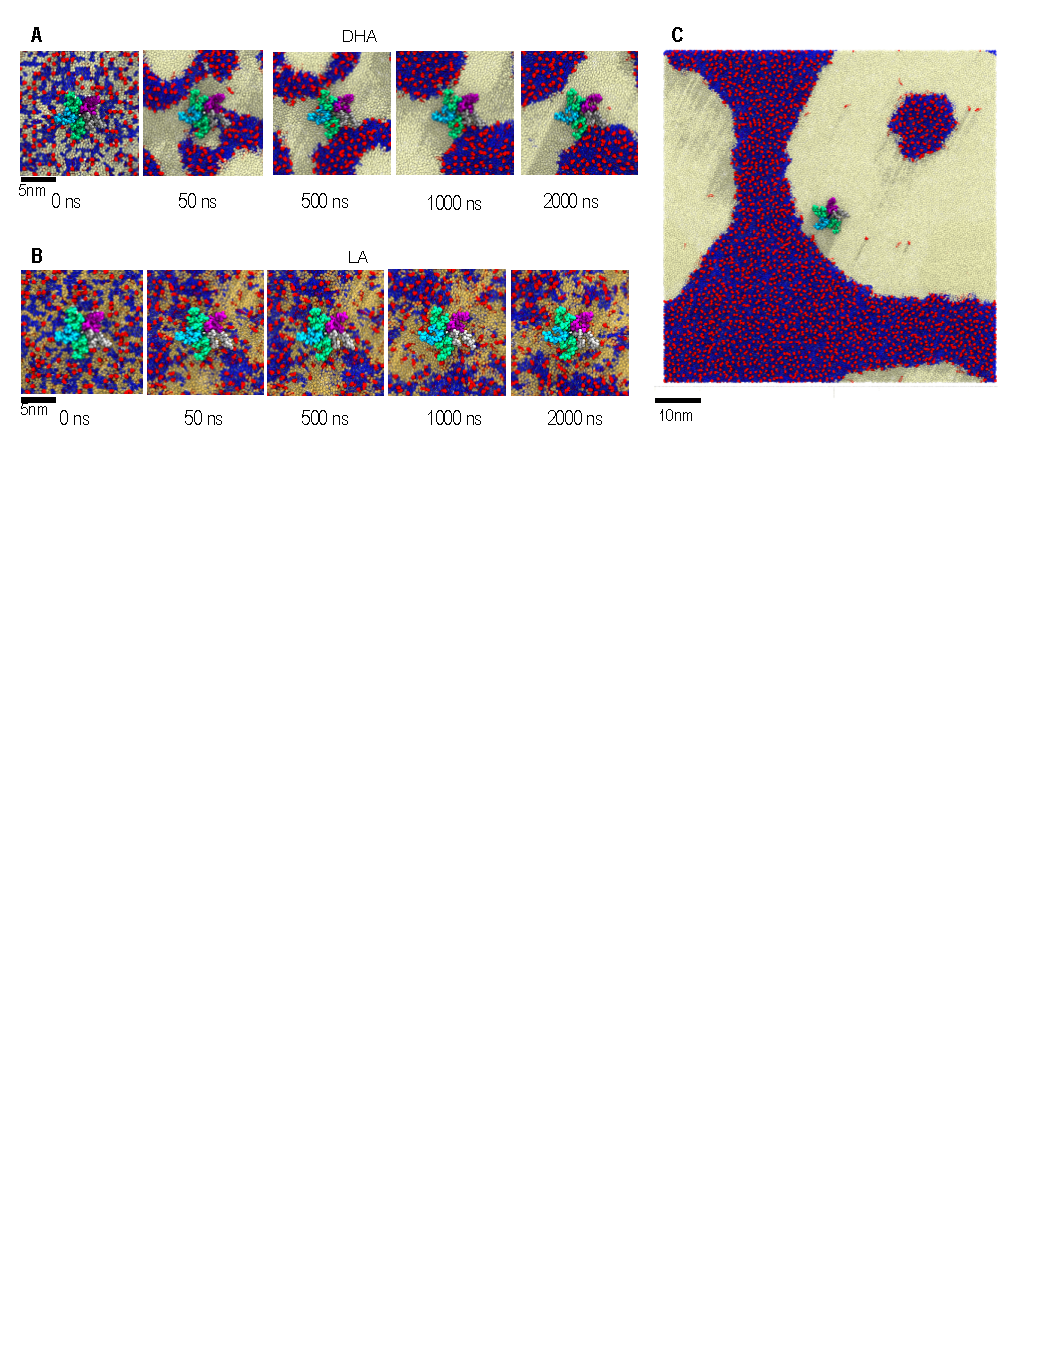
\includegraphics[width=1\linewidth]{ModelMemb_Images/Fig1.pdf}}
		\caption[Trajectories of ternary mixtures at ratios of 2:2:1 DPPC:PUFA:Chol.] {Trajectories of ternary mixtures at ratios of 2:2:1 DPPC:PUFA:Chol. A and B: Trajectories of simulation systems with a single nAChR embedded within small membranes, using lipids containing DHA acyl chains or LA acyl chains. Both simulations were run for 2 $\mu$s. C: Final snapshot of 4 $\mu$s trajectory of a system within a large $\sim$ 75x75 nm$^2$ membrane with the same composition as in A. Subunits are colored: $\alpha$: green, $\beta$: purple, $\delta$: gray, $\gamma$: cyan. Lipids are colored: Chol: red, DPPC: blue, dDHA-PE: white, dLA-PC: tan.}
		\label{fig:fig1}
	\end{figure*}

	\begin{figure}[!ht]
		{
		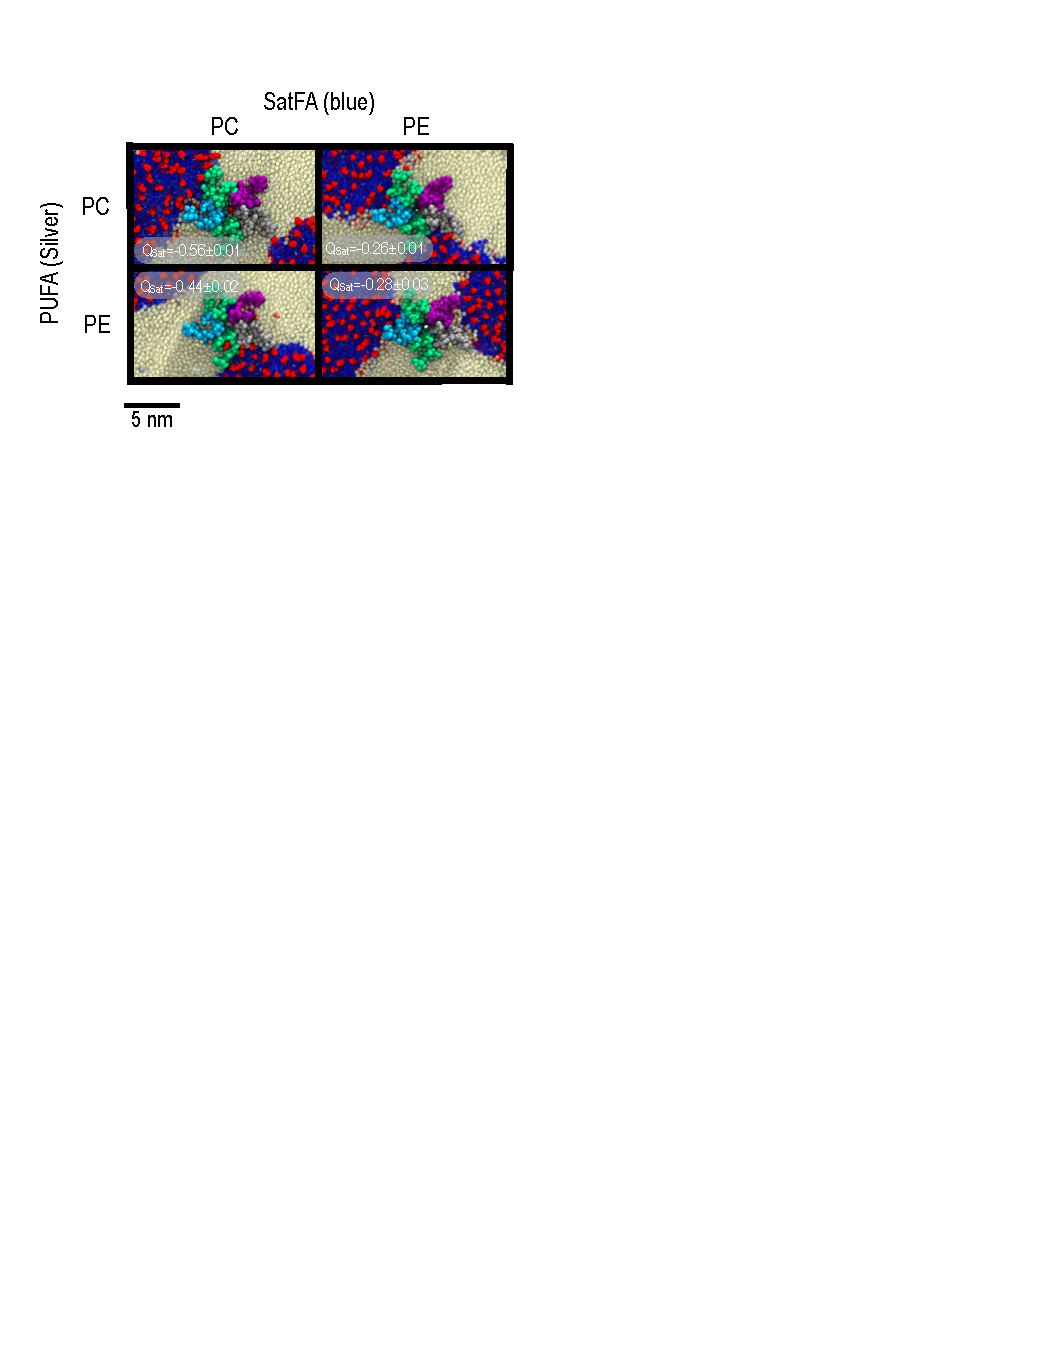
\includegraphics[width=1\linewidth]{ModelMemb_Images/SI_Q.pdf}}
		\caption[ Comparison of nAChR partitioning based on lipid headgroups (PC and PE).] {Comparison of nAChR partitioning based on lipid headgroups (PC and PE). All images represent last frame of 2$\mu$s  simulations of small membranes with composition  2:2:1 Sat:PUFA:Cholesterol.  Rows represent the head-group for the PUFA-containing lipid, while columns represent the head-group of the saturate lipid.   Each image includes $\qsat$ values related to individual systems with errors across averaging 50~ns blocks.}
		\label{fig:SIQ}
	\end{figure}
	Across ternary mixtures with two long $n-3$ PUFA chains (DHA) and a PE headgroup, maximum values of $\mself{DHA}$ approached 5 (Figure \ref{fig:fig2}A), and were significantly reduced (to less than 0.5) when DHA chains were replaced with linoleic acyl (LA) chains. This result is consistent with a previously-observed significant increase in miscibility temperature upon supplementation of plasma membranes with $n-3$ lipids.  \citep{Levental_Polyunsaturated_2016} 
	
	Substantial lipid demixing in DHA-containing mixtures was observed even at low cholesterol concentrations. Over the range we tested, $\mself{DHA}$ was not sensitive to cholesterol concentration $\xch$, as shown by the horizontal contours for DHA in Figure \ref{fig:fig2}A.   

\subsection{nAChR consistently partitions to the liquid disordered domain} \label{PUFA}
	For more than 70 lipid compositions tested, nAChR always partitioned into a PUFA-rich $\ldo$ phase if such a phase was present. We never observed \nachr~partitioning to an $\lo$ phase. Representative frames from trajectories of domain formation in the presence of \nachr~are shown in Figure \ref{fig:fig1}.  This observation includes all tested concentrations of the ternary mixtures, regardless of whether the zwitterionic headgroup was PC or PE (Figure \ref{fig:SIQ}), or whether DPPC was replaced by dioleoylphosphatidylcholine (DOPC) (di-18:1), Palmitoyloleoylphosphatidylcholine (POPC) (16:0,18:1), or dilauroylphosphatidylcholine (DLPC) (di-14:0), as shown in Figure S1.   
	
	{These results are quantified for \nachr~embedded in ternary membranes containing DPPC, CHOL, and either dDHA-PE or dLA-PC in Figure \ref{fig:fig2} B, using the metric $\qsat$ defined in equation \ref{eq:Q}.}  
	In all systems studied here, $\qsat < 0$, indicating depletion of saturated lipids as boundary lipids, consistent with observed partitioning to the $\ldo$ domain in Figure \ref{fig:fig1}. Furthermore, depletion was much stronger in systems containing DHA ($\qsat^{DHA}<< \qsat^{LA}$), consistent with the more well-defined DHA domains ($\mself{DHA}>> \mself{LA}$). 

	\begin{figure}[ht!]
		\center{
		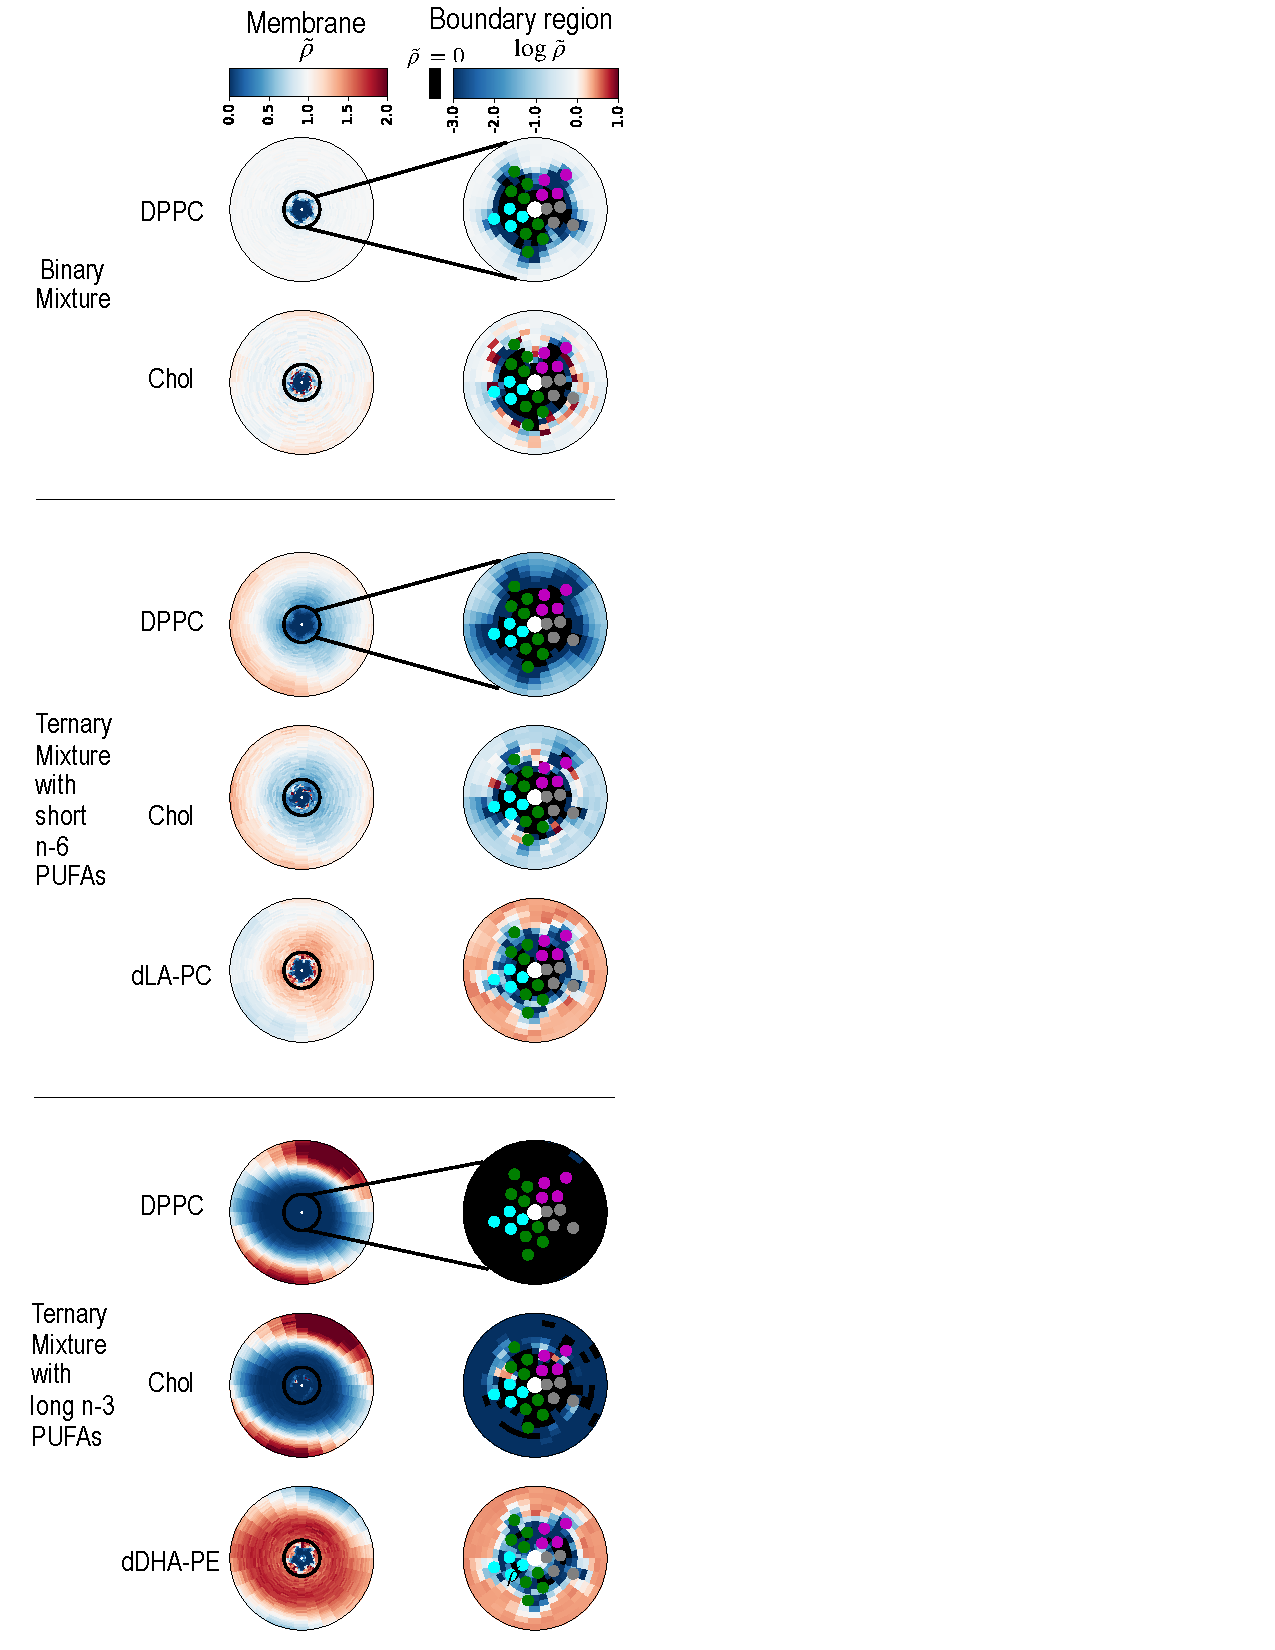
\includegraphics[width=.35\linewidth]{ModelMemb_Images/ComparativeHeatMap.pdf}}
		\begin{flushleft}

		\caption[Lipid density enrichment or depletion around a single central nAChR.] {Lipid density enrichment or depletion around a single central nAChR. Heatmaps are colored according to the normalized density $\tilde{\rho}_{a}$ (left, defined in eq \ref{eq:Rt}) or $\ln\tilde{\rho}_{a}$ (right), averaged over the final 5$\mu s$ of a 10 $\mu s$ simulation. Membrane column (left) depicts density across the simulated membrane; $\tilde{\rho}_{a}<1$ indicates depletion compared to a random mixture, while $\tilde{\rho}_{a}>1$ indicates enrichment. Boundary column (right) shows a zoomed-in region around the protein, with circles corresponding to average position of the protein helices, colored as in Figure \ref{fig:binary}, and black indicating no detected lipid density. If no non-annular or embedded lipid binding was observed, the entire protein footprint would be black for all lipids. Binary mixture contains 4:1 DPPC:CHOL as in Figure \ref{fig:binary}, while both ternary mixtures contain 2:2:1 DPPC:PUFA:Chol.} \label{fig:sorting}

		\end{flushleft}

			\end{figure}
	
	The \nachr~annulus is highly enriched in DHA: DHA-PE constitute nearly 100\% of the local lipids even in membranes with very low DHA concentrations. This strong signal could indicate multiple high affinity sites for DHA chains across the transmembrane protein surface. At another extreme, DHA enrichment could be driven by a very slight preference for DHA in a highly non-ideal bulk: since DHA is found in well-defined domains without protein, even one DHA molecule that binds to the protein surface could stabilize the rest of the $\ldo$ domain nearby. Comparing boundary lipid and domain formation trends can help distinguish between these two scenarios.  If boundary lipid enrichment is determined purely by how well-defined domains are (the latter scenario), we would expect similar trends for $\mself{DHA}$ and $Q_{sat}$ in the DHA column of Figure \ref{fig:fig2}.  In contrast,  Figure \ref{fig:fig2} shows that while domain formation in DHA-containing systems is only weakly sensitive to cholesterol content (horizontal contours), composition of boundary lipids is highly sensitive to cholesterol content (diagonal contours). These results suggest that direct interactions between multiple favorable sites on \nachr and DHA-containing lipids dominate the observed enrichment of DHA among boundary lipids.  
	
	The simulations represented in Figure \ref{fig:fig2} do compare the effects of two unsaturated lipids that also have different headgroups. DHA is far more commonly paired with PE in native membranes, while LA is more commonly found with PC. We found no qualitative differences in \nachr~domain partitioning or significant quantitative effect on $\qsat$ upon switching PC and PE headgroups on the PUFA lipid.  We did observe a quantitative effect of \emph{saturated} lipid headgroup on boundary lipid composition: $\qsat$ was reduced by half when saturated PE was used instead of saturated PC. (Figure \ref{fig:SIQ}).  As shown in Figure \ref{fig:SIQ}, \nachr~is bordered by $\lo$ domains on two opposing faces when saturated PE is used, compared to only one face if PC is used.  
The particular domain topology shown in Figure \ref{fig:SIQ} is an artifact of the periodic boundary conditions, but still indicates more favorable interactions of \nachr~with an $\lo$ domain composed of DPPE vs DPPC. This may reflect a difference in the lipid shape (wedge-shaped DPPE vs cylindrical-shaped DPPC) and the associated monolayer spontaneous curvature.  For PUFA lipids in flexible $\ldo$ domains, lipid shape is less likely to play a significant role in determining partitioning. The dramatic difference in domain flexibility is apparent in  Figure \ref{fig:Memb_Curve}.   
	
	\subsection{Spontaneous integration of lipids into nAChR TMD bundle} \label{Embed}

	The \nachr~structure used for these simulations was determined in a native membrane with a high fraction of polyunsaturated lipids. While we previously \citep{Brannigan2008} proposed that unresolved density in this structure could be embedded cholesterol, the possibility of occupation by phospholipids other than POPC was not investigated.  Furthermore, we did not consider possible asymmetry across subunits in binding previously.  Here we do observe penetration of both the intersubunit (``type B'') and the intrasubunit (``type A/C'') sites previously proposed\citep{Brannigan2008}, by both phospholipids and cholesterol, but with a high degree of subunit specificity.  
		
Two dimensional density distributions of DPPC, PUFAs, and cholesterol over short and long length scales were measured for two ternary mixtures and one binary mixture (Figure \ref{fig:sorting}).   In binary DPPC/cholesterol membranes, DPPC was more likely than cholesterol to occupy intrasubunit sites.  DPPC binds shallowly in the $\alpha$ subunit and more deeply in the $\beta$ subunit. Introducing PUFAs resulted in displacement of both cholesterol and DPPC from intrasubunit sites, except for the $\beta$ intrasubunit site, which became more likely to be occupied by cholesterol. The interior of the $\beta$ subunit TMD has the largest amount of available volume, could sequester cholesterol (but not DPPC) from the PUFA lipids in the annulus, and filling the interior with a PUFA chain may be entropically costly.  PUFA chains did occupy other intrasubunit sites, but remained fluid, as shown in Figure \ref{fig:sum}. 

	Intersubunit sites were rarely occupied by DPPC, with the exception of the $\beta+/\alpha-$ site in the binary system (Figure \ref{fig:sorting}). Intersubunit sites were more likely to bind cholesterol, particularly the $\beta+/\alpha-$, $\alpha+/\gamma-$, and $\alpha+/\delta-$ subunit interfaces. Occupation of the $\alpha+/\delta-$ interface is consistent with cryo-EM observations\citep{Unwin2017}  of enhanced cholesterol density around the $\alpha+/\delta-$ site. Intersubunit sites that were not significantly occupied by cholesterol ($\delta+/\beta-$ and $\gamma-/\alpha+$) did show significant and deep occupation by DHA, which tended to enter from the adjacent intrasubunit site rather than from the membrane. Even those intersubunit sites with significant cholesterol occupancy can simultaneously bind part of a DHA chain, yielding non-vanishing DHA density.  

	\subsection{Lipid sorting over the 5-20 nm range is associated with larger domains  } \label{Sorting}

	We also calculated density distributions of each lipid species at distances beyond the ``annular'' ring, over the 5-20 nm range.    As shown in Figure \ref{fig:sorting} (left column), observed sorting of lipids within {5-20~nm} of the \nachr~is dependent on the overall composition of the membrane. For all compositions shown, cholesterol is depleted within 5-20~nm and enriched even farther from the protein.  Within the binary systems this effect is minor ( $\tilde\rho_{CHOL} \sim 1$), but it becomes stronger in the moderately demixed LA systems ($\tilde\rho_{CHOL} \sim 0.5$) and substantial ($\tilde\rho_{CHOL} \sim 0.25$) for the highly-segregated DHA containing systems.  A similar pattern is observed for DPPC, which suggests that ``sorting'' over the 5-20~nm range is primarily driven by intrinsic differences in membrane organization that would be observed without the receptor. PUFAs are also most highly enriched at intermediate distances : the deepest red band is found at about 5~nm~in LA-containing systems and about 8~nm~ in DHA-containing systems.  This would be expected when \nachr~partitions near a curved domain boundary, as in Figure \ref{fig:SIQ}.      			

	\begin{figure}[h!]
		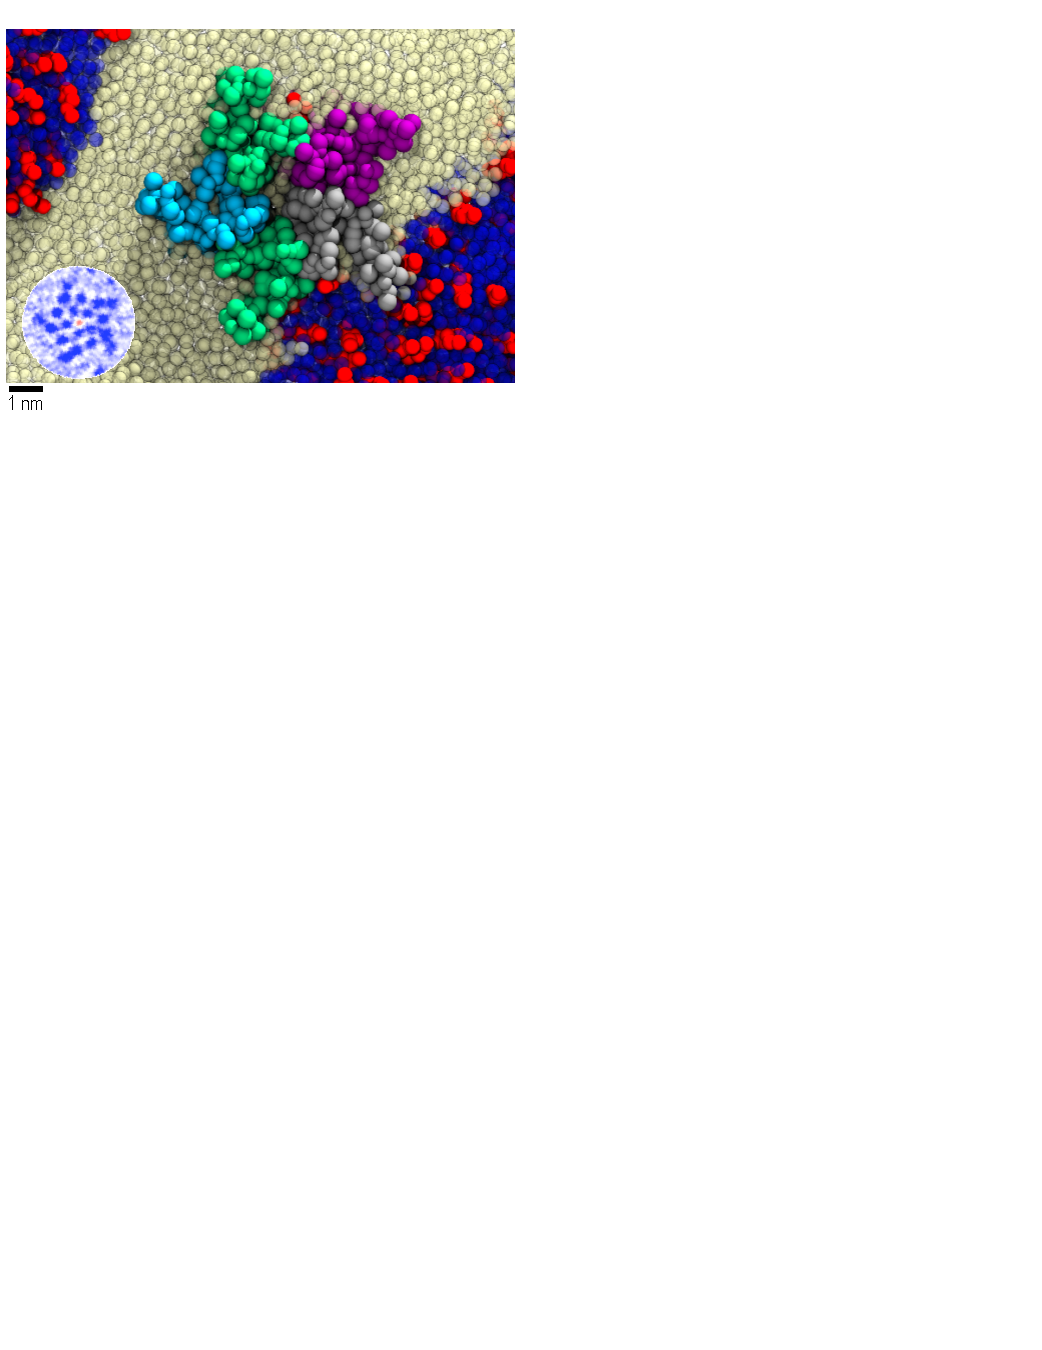
\includegraphics[width=1\linewidth]{ModelMemb_Images/Summary.pdf}
		\caption[Embedded lipids in the nAChR.] {Embedded lipids in the nAChR. Main image: Representative frame from equilibrated small membrane simulation of nAChR in 2:2:1 DPPC:DHA-PE:CHOL. Backbone beads of the TMD helices are colored by subunit as in Figure \ref{fig:fig2}; side-chain beads are not shown.  Both DHA-PE (white) and cholesterol (red) equilibrate to embedded sites in the subunit center and subunit interfaces, although most cholesterol is found in the $\lo$ phase with DPPC (blue). Inset : Cryo-EM density of nAChR from \citep{Miyazawa2003} as rendered in \citep{Brannigan2008}; dark blue indicates high density, white is medium density, and red is low density. }
		\label{fig:sum}
	\end{figure}

	 
 \section{Discussion}
\label{S:4}

In this work we used coarse-grained simulations to predict the local lipid composition around the nicotinic acetylcholine receptor, in a range of domain forming membranes.  We observed  \nachr~partitioning to the liquid-disordered phase in all systems for which such a phase was present.  This is inconsistent with the model of lipid rafts as platforms that contain a high density of nAChRs, and unexpected in light of the established cholesterol dependence of nAChR.  As shown in these simulations, partitioning to the $\ldo$ phase does not prevent \nachr~from accessing cholesterol. 

The simulations presented here involve only one receptor per system.  Using the present results only, the simplest extrapolation to multiple receptors would assume that receptors are simply distributed randomly across the $\ldo$ domain.  The local receptor area density would be the number of receptors divided by the total area of $\ldo$ domains.    

In the model membranes used here, as well as in native nAChR membranes, the lipid composition would be expected to yield $\ldo$ phases that were about the same size as $\lo$ phases. The $\lo$ ``raft'' in an $\ldo$ ``sea'' analogy is not representative when over 50\% of the membrane is in the ``raft'' phase.  A more representative analogy would be receptors as boats, floating on an $\ldo$ lake within an $\lo$ rigid land mass.  Filling in the lake by adding to the coastline would force any boats in the lake closer together.  Similarly, any process that decreased total $\ldo$ area while keeping the number of receptors constant would increase the local receptor density.   In this model, observing increased \nachr~density by adding membrane cholesterol (as in \citep{Barrantes2000,
Barrantes2014,Bruses2001,Marchand2002,Oshikawa2003,Pato2008,Zhu2006a, Barrantes2007,Wenz2005,Borroni2016}) would be consistent with \nachr~partitioning to the cholesterol-poor phase rather than the cholesterol-rich phase. 

This extrapolation from a single receptor assumes that introduction of additional receptors does not change partitioning behavior.  We do still find reliable partitioning to the $\ldo$ phase upon adding more receptors, and we will characterize systems with multiple receptors in a future publication. Due to receptor dimerization and trimerization, distribution of individual receptors within the $\ldo$ phase will not be random.   This would not change the expected trend of density increasing with added cholesterol, however.  This interpretation also assumes that cholesterol is randomly mixed within the $\lo$ phase, while results from atomistic simulations\citep{Sodt2014, Iyer2018} have suggested that cholesterol may preferentially partition to the boundary between $\lo$ phases and $\ldo$ phases composed of monounsaturated lipids. Similar studies in which the $\ldo$ domain is composed of PUFAs and the interface is much more compact have not been reported.  In the present coarse-grained simulations, we did observe random mixing of cholesterol within $\lo$ phases, rather than at the boundary with the PUFA-rich $\ldo$ phase.  

Observed partitioning into the $\ldo$ phase could be considered inconsistent with interpretations of some experiments, \citep{Bermdez_Partition_2010,Perillo2016} which suggest minimal nAChR partitioning preference in symmetric model membranes or an actual preference for an $\lo$ phase in asymmetric model membranes.  These experiments used only monounsaturated acyl chains, and may have had less well-defined domains.  They further relied on detergent resistant membrane (DRM) methods, which are sensitive to {the} choice of detergent \citep{Brown2007} and could be unable to distinguish between proteins with no partitioning preference vs proteins that persistently partition to one side of a boundary. 

The origin of preferential partitioning observed in these simulations for the $\ldo$ domain is still unclear, but may reflect different elastic properties of the $\ldo$ and $\lo$ domains.  In general, proteins embedded in membranes will introduce a boundary condition on the membrane shape, such that (1) the thickness of the membrane matches the thickness of the transmembrane domain\citep{Aranda-Espinoza1996, Jensen2004, Brannigan2005a} and (2) interfacial lipids are parallel to the protein surface.\citep{Goulian1993}.  Transmembrane proteins with hydrophobic mismatch with the surrounding membrane may deform the membrane thickness to satisfy constraint (1), while cone-shaped proteins like pLGICs~ must also introduce a ``tilt'' deformation to satisfy (2).  Each leaflet of the membrane has an elastic resistance to bending away from its spontaneous curvature, and satisfying these constraints is energetically costly.  

Continuum theories based on the Helfrich Hamiltonian have been used to predict shape deformations around protein inclusions in homogeneous membranes \citep{Goulian1993,Aranda-Espinoza1996,Brannigan_A_2006}.  In mixed membranes, minimization of the protein-deformation free energy may also induce lipid sorting.  Two distinct sorting mechanisms could minimize the bending free energy: sorting that A) reduces the required bending deformation, by selecting boundary lipids with a specific thickness, leaflet asymmetry, or shape or B) reduces the free energy cost of the bending deformation, by selecting for flexible boundary lipids.   Mechanism (B) is the most generally applicable approach, and would stabilize partitioning to the most flexible domains, consistent with our observations (Figure \ref{fig:Memb_Curve}).  In some cases, mechanism (A) may also contribute to partitioning or lipid-sorting, and could explain why \nachr~tends to attract saturated PE over saturated PC, or how leaflet asymmetry can promote partitioning to more rigid phases as observed in \citep{Perillo2016} . 

We previously \citep{Brannigan2008} proposed unresolved density in the cryo-EM structure of \nachr~ in the {\it Torpedo} membrane could be embedded cholesterol, based on gain of function caused by cholesterol in reconstitution mixtures\citep{Fong1986,Sunshine1992,Hamouda2006,Butler1993,Bhushan1993,Fong1987,Bednarczyk_Transmembrane_2002,Corrie_Lipid_2002}, but we did not consider the possibility of occupation by polyunsaturated chains.  
Here we observe spontaneous binding of cholesterol to coarse-grained embedded sites, but long-chain PUFA tails displace cholesterol in some binding sites. Long acyl chains may penetrate far into the TMD bundle without requiring the entire head group also be incorporated, and long-chain PUFAs may do so without as substantial an entropic penalty as long saturated chains.  Cholesterol (like phosphatidic acid, another lipid known to cause gain of function under some preparations\citep{Butler1993,Bhushan1993,Fong1987,Bednarczyk2002,Corrie_Lipid_2002})  has a much smaller headgroup than PC or PE. It can become fully incorporated into the TMD without the TMD needing to accommodate the bulky headgroup.   These complex associations underlie the challenges of predicting local lipid environment in heterogeneous, highly non-ideal mixtures. 

All simulations reported here contain lipids with di-saturated tails or di-PUFA tails. While lipid species with two identical acyl chains do exist in the native membrane, they are far less common than hybrid lipids with heterogeneous acyl chains.  Including hybrid lipids would reduce the potential for formation of large domains, while increasing the length of the domain interface. 
Incorporation of hybrid lipids would also reduce the \nachr-local concentration of PUFA chains.  Even 5-10\% DHA is a saturating concentration for \nachr~cavities, however, so we expect occupation of cavities to be minimally affected by replacement of di-DHA lipids with twice the number of hybrid lipids. 

None of the three generations of experimental studies into the effects of cholesterol and lipid headgroup on \nachr~function have systematically considered the effects of lipid polyunsaturation. We predict that first-generation-style functional studies would find that \nachr s reconstituted in model membranes are sensitive to replacement of even a small fraction of saturated or mono/diunsaturated acyl chains with $n-6$ and (especially) $n-3$ PUFAs. Within domain forming membranes common to second-generation studies, systematically varying polyunsaturation and phospholipid topology could help untangle the effect of direct interactions vs organization, as we discussed in \citep{Brannigan2017}. Third-generation structural biology techniques are the most promising approaches for detecting subunit-specific interactions. While it is unlikely that polyunsaturated acyl chains could be resolved, lipids could be chosen such that particular chains also had a unique and resolvable headgroups. In general, modular lipid topology allows for numerous strategically-designed experiments to isolate the role of head-group versus acyl chain in determining boundary lipids. 

\chapter{Untangling direct and domain-mediated interactions between nicotinic acetylcholine receptors in DHA-rich membranes}
Originally published in: Journal of Membrane Biology, 2019, vol. 252, pages 385-396\\ \\ 
%%example: \kwn{sup}


%\setcounter{savepage}{\thepage}

Kristen Woods*$^1$, Liam Sharp*$^1$, Grace Brannigan$^{1,2}$
{1) Center for Computational and Integrative Biology, Rutgers University-Camden, Camden, NJ}  {2) Department of Physics, Rutgers University-Camden, Camden, NJ}
*These authors contributed equally.

\section{Abstract}

Lipid composition of the membrane can strongly modulate both function and organization of the nicotinic acetylcholine receptor (nAChR). Previously we conducted coarse-grained molecular simulations of a single nAChR from the electric ray {\it torpedo} in mixed membranes, and observed that lipids containing long chain polyunsaturated fatty acids (PUFAs) like docosahexaenoic acid (DHA) were abundant among nAChR boundary lipids.   Using a similar approach to investigate the role of lipid topology and lipid domain formation, here
%At the neuromuscular junction, the nicotinic acetylcholine receptor (nAChR) self-associates to give rise to rapid muscle movement. While lipid domains have maintained nAChR aggregates in-vitro, their specific roles in nAChR clustering are currently unknown. In the present study, we carried out coarse-grained molecular dynamics simulations (CG-MD) of 1-4 nAChR molecules in two membrane environments: One mixture containing domain-forming, homoacidic lipids, and a second mixture consisting of heteroacidic lipids. Spontaneous dimerization of nAChRs was up to ten times more likely in domain-forming membranes; however, the effect was not significant in four-protein systems, suggesting that lipid domains are less critical to nAChR oligomerization when protein concentration is higher. With regard to lipid preferences, nAChRs consistently partitioned into liquid-disordered domains occupied by the omega-3 fatty acid, Docosahexaenoic acid (DHA); enrichment of DHA boundary lipids increased with protein concentration, particularly in homoacidic membranes. This result suggests dimer formation blocks access of saturated chains and cholesterol, but not polyunsaturated chains, to boundary lipid sites.
 
 
  
 
 
 
 
 
% At the neuromuscular junction (NMJ), the nicotinic acetylcholine receptor (nAChR) self-associates to give rise to rapid muscle movement. While lipid domains have maintained nAChR aggregates in-vitro, their specific roles in nAChR clustering are currently unknown. In the present study, we carried out coarse-grained molecular dynamics simulations (CG-MD) of 1-4 nAChR molecules in two membrane environments: One mixture containing domain-forming, homoacidic lipids, and a second mixture consisting of heteroacidic lipids. Spontaneous dimerization of nAChRs was up to ten times more likely in domain-forming membranes; however, the effect was not significant in four-protein systems, suggesting that lipid domains are less critical to nAChR oligomerization when protein concentration is higher. With regard to lipid preferences, nAChRs consistently partitioned into liquid-disordered domains occupied by the omega-3 ($\omega$-3) fatty acid, Docosahexaenoic acid (DHA); enrichment of DHA boundary lipids increased with protein concentration, particularly in homoacidic membranes. This result suggests dimer formation blocks access of saturated chains and cholesterol, but not polyunsaturated chains, to boundary lipid sites.   

%{ The nicotinic acetylcholine receptors (nAChR) are highly lipid sensitive pentameric ligand gated ion channels that agrigate into dense clusters, hypothesized to be driven by domain formation. We showed previously using coarse grained simulations\citep{Sharp2019} the nAChR domain partitioning, as well as annular and non-annular lipid interaction, are highly regulated by polyunsaturated fatty acids (PUFAs). Here, using coarse grained molecular dynamics, we investigated multiple replicas of membranes with one to four embedded nAChRs to try and resolve the effect of naChR clustering due to quasi-native membrane composition. All simulations had constant ratios of saturated fatty acids, PUFAs, and cholesterol; however domain forming membranes used lipids with homoacids (three lipid species), while non-domain forming membranes used lipids heteroacids (two lipid species). Results  show variation between both domain forming and non-domain forming membranes and thier lipids direct interaction with nAChR. More interestingly differences in direct interactions between lipids and one or more proteins are observed.  Specifically we see changes in annular lipids and embedded lipids distributions, distances between nAChR-nAChR pairs, and nAChR subunit-nAChR subunit interactions.}
%\end{abstract}
%\setcounter{page}{\thesavepage}
%\stepcounter{page}

\section{Introduction}
\label{intro}
%Your text comes here. Separate text sections with
%\section{Neuromuscular nicotinic acetylcholine receptors (nAChRs) and their lipid interactions}
%\label{sec:1}
The muscle-derived nicotinic acetylcholine receptor (nAChR) (PDB 2BG9) \citep{Unwin2005} is the most abundant neurotransmitter receptor at the neuromuscular junction (NMJ) in most vertebrates, including humans \citep{Albuquerque2009}. Within the postsynaptic membrane, nAChRs cluster in high densities (10,000 per $\mu$m$^{2}$) to properly activate the skeletal muscle \citep{Ramarao1998,Breckenridge1972}. As a major transmembrane protein, nAChR depends upon a highly specific lipid environment to maintain functionality. Lipids influence nAChR activity by affecting both function and organization. It is essential to understand how changes in lipid environment impact nAChR's structure and activity, given that lipids can change in response to aging and disease  \citep{Yadav2014}, and also vary across tissue and organism. 



Over the past few decades, considerable progress has been made in uncovering lipid sensitivities associated with nAChR \citep{Criado1982}. In a majority of experiments, researchers have prioritized studying cholesterol over other membrane lipids. Early studies revealed that, when reconstituted into membrane mixtures, nAChR failed to conduct cations across the lipid bilayer unless cholesterol was present  \citep{Fong1986,Sunshine1992,Butler1993,Fong1987,Corrie2002}. 
%\section{Subsection title}
%\label{sec:2}
%as required. Don't forget to give each section
%and subsection a unique label (see Sect.~\ref{sec:1}).
%\section{nAChR clustering in association to lipid rafts}
More recently, researchers have examined the effects of membrane dynamics on nAChR organization \citep{Baenziger2015,Bruses2001,Marchand2002,Oshikawa2003,Pato2008,Zhu2006a,Baenziger2017,Barrantes2007,Barrantes2000,Bermudez2010,Barrantes2010,Perillo2016,Wenz2005,Borroni2016,Unwin2017}. In-vitro studies \citep{Barrantes2007,Barrantes2010} indicate that nAChRs form larger aggregates upon cholesterol depletion. Experimental evidence suggest that cholesterol-rich lipid domains, known as lipid rafts, facilitate clustering of nAChRs \citep{Campagna2006,Marchand2002,Pato2008}. 
More specifically, after disrupting lipid raft formation, Zhu et al. observed a significant loss of nAChR clusters in-vitro \citep{Zhu2006a}. In the mature neuromuscular membrane, nAChRs are linked by the intracellular anchoring protein, rapsyn, which bridges receptors together at their bases  \citep{Zuber2013a}. According to fluorescent studies \citep{Marchand2002}, lipid rafts mediate the association between rapsyn and neighboring nAChR molecules. In the mid-2000's, Willmann et al. and Stetzkowski-Marden et al. proposed that lipid rafts can stabilize receptor networks and may even provide a localized environment for nAChR \citep{Willmann2006,Stetzkowski-Marden2006}. 

Domain formation occurs when a membrane is comprised of at least three lipid types: cholesterol, unsaturated fatty acids, and a molecule that interacts closely with cholesterol such as saturated fatty acids or sphingomyelin \citep{Feller_Acyl_2008,Yeagle2016115}.  The membrane separates into at least two domains, a liquid-ordered or ``raft'' phase containing cholesterol and saturated lipids/sphingomyelin, and a liquid-disordered phase containing unsaturated lipids. Polyunsaturated phospholipids make these domains more well-defined \citep{Levental_Polyunsaturated_2016}. Some results from atomistic simulations \citep{Sodt2014, Iyer2018} indicate that cholesterol may preferentially partition to the boundary between liquid-ordered phases and liquid-disordered phases composed of monounsaturated lipids.  In neuromuscular membranes, intrinsic domain formation is dependent upon several lipid species, including the widely influential omega-3 ($\omega$-3) fatty acids. One $\omega$-3 in particular, Docosahexaenoic acid (DHA), is prevalent in the native neuromuscular membrane and is strongly associated with flexible and well-defined domains  \citep{Turk2013,Shaikh2004}. Additionally, DHA is a major contributor to brain functioning, motor activity, and cardiac health; however, its specific effects on neuromuscular health are poorly understood \citep{12439486320170901,S000930840800032720080101,Georgieva2015}. 

\begin{figure}[htp]
\center
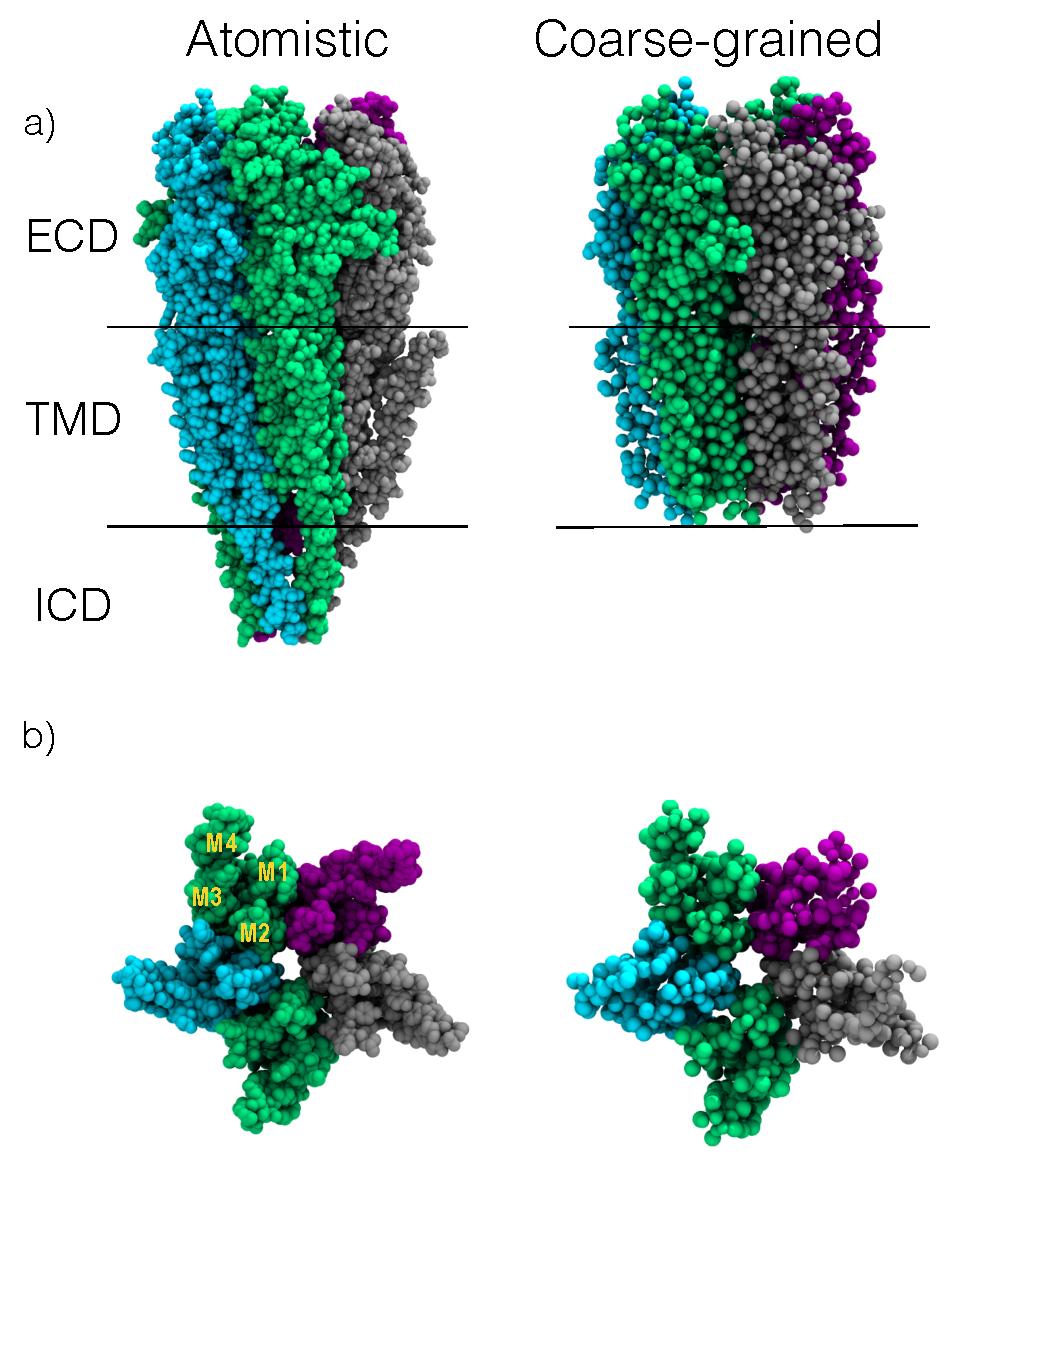
\includegraphics[width=.75\columnwidth,]{figure/figure1.pdf}
	\begin{flushleft}

\caption[Nicotinic acetylcholine receptor (nAChR) structure] {Nicotinic acetylcholine receptor (nAChR) structure. a) Atomistic and coarse-grained representations of Unwin et al's cryo-EM structure, PDB 2BG9. The nAChR is colored by subunit ($\alpha:green,\beta:purple,\delta:gray,\gamma:cyan$) and labeled by structure. The extracellular domain (ECD) is located above the bilayer and is critical for ligand-binding. The transmembrane domain (TMD) is positioned within the lipid bilayer, and the intracellular domain (ICD) is located in the cytoplasm. The coarse-grained model omits the ICD since it is poorly resolved and not necessary for this study. b) TMD from the extracellular perspective, with its four alpha helices labelled in a single $\alpha$ subunit. The outermost M4 helices closely interact with surrounding membrane lipids, while the M2 helices outline the ion pore; the M1 and M3 helices make up the body of the transmembrane domain \citep{Unwin2005}.}
	\end{flushleft}

  \label{fig:structure}
\end{figure}


Characterizing such complex lipid-protein interactions requires detailed information on each molecular structure. The nAChR is a member of a family of ion channels, known as pentameric ligand-gated ion channels (pLGICs), which has a number of recent structures \citep{Laverty2019,Laverty2017,Masiulis2019,Althoff2014,Hibbs2011,Morales2016,Baenziger2011,Corringer2012,S089662731630023X20160504,Prevost2012a,Sauguet2014}; however, only single structures have been determined, rather than dimers. pLGICs are composed of five subunits; each subunit is composed of an extracellular domain for ligand binding, a transmembrane domain (TMD), and an intracellular domain (ICD) (Figure 1A). The TMD is the embedded portion of pLGICs that interacts most often with surrounding membrane lipids; this region of pLGICs is composed of four alpha-helices, M1-M4, with the innermost, M2 helices forming the ion pore. The ICD, or cytoplasmic domain, is highly disordered, making it challenging to obtain information on its structure. Currently, there are two structures of nAChR pentamers resolved from x-ray crystallography (neuronal type) and cryo-electron microscopy (muscle-type) \citep{Morales2016, Unwin2005}.

Other closely related channels have been resolved with bound lipids. In 2017, the inhibitory neurotransmitter receptor, the gamma-aminobutyric acid (GABA$_A$) receptor, was crystallized with a cholesterol molecule protruding between its M1 and M3 helices \citep{Laverty2017}, similar to our previous prediction \citep{Hnin_A_2014}. Interestingly, x-ray structures of the glutamate-gated chloride channel (GluCl) revealed embedded POPC phospholipids in the same location \citep{Althoff2014}. Together, these data provide evidence for lipid-based modulation of pLGICs, which can potentially be applied to the gating of nAChR.

Structural information alone, however, is insufficient for answering questions about native cell membranes. For one, most structures are obtained under artificial conditions, using detergents or nanodisks with non-native lipid composition. Additionally, current structures do not represent oligomers, particularly in a liquid state. Fully atomistic molecular dynamics (MD) simulations \citep{brannigan, Cheng2009, Hnin_A_2014, Carswell_Role_2015} have complemented experimental investigations of pLGICs interacting with lipids, but they are limited in their ability to capture domain formation since atomistic lipids cannot diffuse over typical simulation microsecond time scales \citep{Ingolfsson2014,Bond2006,Parton2013,Goose2013,Scott2008}.  Furthermore, it is unfeasible to incorporate multiple nAChRs in simulations with atomistic resolution. Coarse-grained MD (CG-MD) simulations are run over longer length and time scales, making them suitable for exploring complex model membranes. CG-MD is widely applied in simulations of both lipid-protein binding and domain formation \citep{Bond2006,Scott2008,Parton2013,Goose2013}. Additionally, CG-MD can capture large-scale membrane phenomenon such as protein self-assembly and lipid-mediated oligomerization \citep{10.3389/fphys.2016.00494, BAADEN2013878}.

Recently, we \citep{Sharp2019} conducted CG-MD simulations of a single nAChR from the electric ray {\it Torpedo} in mixed membranes. Contrary to expectations, nAChR consistently preferred a local lipid environment rich in PUFAs rather than cholesterol, especially long-chained $\omega$-3s, such as DHA. While cholesterol occupied the transmembrane gaps of nAChR, PUFAs were even more likely to be embedded, regardless of their phospholipid headgroup. 

The present study adopts a similar approach, with a particular focus on nAChR-associated clustering. Through molecular dynamics simulations, we investigate nAChR lipid preferences and clustering behavior in membranes with and without domains. For this study, we tested three major hypotheses: 1) Membrane organization affects nAChR boundary lipid specificity: when PUFA chains are prevented from forming PUFA rich domains, their prevalence among nAChR boundary lipids will be significantly reduced. 2) Domain formation will indirectly facilitate the clustering of nAChRs, by inducing partitioning preferences and restricting diffusion within the membrane. 3) Within a dimer, we will observe sequence preferences in facing subunits.
%\paragraph{Paragraph headings} Use paragraph headings as needed.
\section{Methods}
\subsection{System setup}

In order to isolate the role of lipid domain formation on nAChR-based lipid sorting and clustering, our simulations compared two different membranes with distinct phospholipid topology. Each membrane had 30\% cholesterol and 70\% phospholipids.  The phospholipids all had phosphatidylcholine (PC) headgroups, and half the total number of acyl chains were saturated (16:0) chains, while the other half were polyunsaturated (22:6) chains.  For homoacid membranes, all phospholipids had either two polyunsaturated acyl chains (didocosahexaenoylphosphatidylcholine or dDHA-PC) or two saturated chains (dipalmitoylphosphatidylcholine or DPPC), facilitating domain-formation. In the heteroacid membranes, all phospholipids were hybrid lipids with one polyunsaturated acyl chain and one saturated chain (1-palmitoyl- 2-docosahexaenoyl- phosphatidylcholine or PDPC), which are topologically unable to separate into PUFA-rich and PUFA-poor domains. 

Lipids and proteins were modeled using the coarse-grained (CG) Martini 2.2 force field \citep{martini}. % Use of the coarse-grained force field allowed us to observe large-scale membrane interactions that are inaccessible through all-atomistic approaches (AA); such interactions include domain formation, protein partitioning, and protein clustering.By using a CG model, we could run simulations for longer length and time scales, with systems approaching equilibrium at approximately 2 $\mu$s.  \citep{Marrink2007} 
Systems included between 1-4 nAChR molecules, derived from the Torpedo electric organ \citep{Unwin2005} (PDB 2BG9).  This structure is the only pLGIC structure obtained in a native membrane. % One membrane had intrinsic domain formation, due to its fully saturated and fully unsaturated phospholipids: 35:35:30 Di-palmitoyl phosphatidylcholine (DPPC): Di-docosahexaenoyl\\ phosphatidylcholine (DHA-PC): Cholesterol. In a second composition, domain formation was prevented by using a mixture of hybrid lipids, each with one DHA and one saturated tail: 70:30 1-palmitoyl-2-docosahexaenoyl-phosphatidylcholine (PUPC): Cholesterol. \citep{Marrink2007}

We converted protein structures into CG models using the Martini script "martinize.py", mapping four non-hydrogen atoms to one CG interaction. We constructed and assembled our protein-bilayer systems using  the Martini script, "insane.py", using a box sizes of 29x29x21 nm$^{3}$ for one-to-two proteins, 40x40x20 nm$^{3}$ for three proteins, and 44x44x22 nm$^{3}$ for four protein systems, respectively  \citep{Marrink2007}. Initially, the proteins were in a circle of about 13 nm. The receptors were evenly spaced, and their $\delta$ subunits were facing the same direction. Once simulations started, nAChRs shifted from their initial orientations. We ran 24 CG-MD simulations containing 1-4 nAChRs (3 replicas per system). 

\subsection{Simulation details}
Simulations were run using the Martini 2.2 force field parameters and the Gromacs 5.1.2 simulation package, \citep{Marrink2007,Pronk2013} as in our previous work, \citep{Sharp2019}. Each simulation consisted of two steps: energy minimization and molecular dynamics. {For each system, we ran two consecutive energy minimizations for 10,000 steps. }%For each system, we ran two consecutive equilibrium simulations for 10,000 steps at a 0.001 ps time-step.  
Harmonic restraints between backbone atoms were imposed to preserve nAChR conformation. 
More specifically, we applied an elastic force constant of 750 kJ/mol and set lower and upper bounds on the bond with using a bond length of 0.7 nm
%lengths 0.9 nm and 1.6 nm, 
 \citep{Marrink2007,Pronk2013}. The molecular dynamics simulations ran for 10-20 $\mu$s at a 0.025 ps time-step. Simulation temperature and pressure were kept constant at values of 323 K and a reference pressure of 1 bar. The isotropic pressure coupling compressibility constant was maintained at 3.0 $\times {10^{-5}}$ bar$^{-1}$. 

% rephrase using the information from Liam's paper below (commented out)

%All simulations were run using a isothermal-isobaric (NPT) ensemble, with a Berendsen thermostat of 323 K and a temperature coupling constant of 1 ps, as well as isotropic pressure coupling with compressibility set to $3\times 10^{-5}$ bar$^{-1}$ and a pressure coupling constant set to 3.0 ps.

\subsection{Analysis}
%First, we quantified the degree of protein partitioning within a lipid domain by counting the number of $b$ boundary lipids and comparing it with its expectation in a randomly mixed membrane. In the case of saturated lipids, the metric $Q$ can be written as follows:

For a given nAChR, $\bemb^{\alpha}$ is the total number of embedded lipids of lipid species $\alpha$, where embedded lipids satisfy the following criteria: the headgroup (in the case of cholesterol) or the terminal bead on the acyl chains (in the case of phospholipids) are within 10 {\AA}~of the M2 helices. Visual inspection indicated any lipids outside of this range were also outside of the TMD bundle.

Similarly, $\bann^{\alpha}$ is the total number of annular lipids of lipid species $\alpha$, where annular lipids satisfy the following criteria:  headgroup or the terminal bead on the acyl chains is between 10 {\AA}~and 35 {\AA}~of the M2 helices. This range of lipids corresponded to the third lipidation shell around nAChR.

(For phospholipids, each acyl chain was counted separately as a half-lipid, so it was possible for e.g. the sn-1 chain to be embedded and the sn-2 chain to be annular. )

Boundary lipid fractions for a given species $\alpha$ are defined as 
\begin{eqnarray}
      \femb^{\alpha}&\equiv \frac{  \bemb^{\alpha} }{\bemb },\\
      \fann^{\alpha}&\equiv \frac{\bann^{\alpha}}{\bann}
    \label{eq:f}
  \end{eqnarray}
where $\bemb$ and $\bann$ are the total number of embedded and annular lipids, respectively.  

Two dimensional density distributions of boundary acyl chain species (B), $\tilde{\rho}_{B}(r_i,\theta_j)$ were calculated, as a function of radius, $r_i$, and angle $\theta_j$ projected onto the membrane.

  \begin{equation}
 %   \begin{aligned}
      \rho_{B}(r_i,\theta_j)= \frac{\left\langle n_{B}(r_i,\theta_j) \right\rangle}{r_i \Delta{r}\Delta{\theta}} \\        
   % \end{aligned}
    \label{eq:R}
  \end{equation}

where $r_i = i \Delta r$ is the distance from the origin to the center of bin i, $\Delta r$ is the radial bin width, and $\Delta \theta$ is the angular bin width. $\left\langle n_{B}(r_i,\theta_j) \right\rangle$ is the time-averaged number of acyl chain beads of species B within bin i.

To quantify enrichment or depletion of a given acyl chain with respect to random distribution, the normalized density, $ \tilde{\rho}_{B}(r_i,\theta_j)$, was calculated.

  \begin{equation}
 %   \begin{aligned}
  \tilde{\rho}_{B}(r_i,\theta_j)=\frac{ \rho_{B}(r_i,\theta_j)}{x_{B}s_{B}~N_{L}/\langle L^{2}\rangle} \\        
 %   \end{aligned}
    \label{eq:Rt}
  \end{equation}
  
  where $s_B$ is the number of beads of lipid species B, $N_L$ is total number of lipids in a system, and $\langle L^{2}\rangle$ is the average projected box area, and $x_B$ is lipid B concentration. The expression does not take into consideration the protein footprint or undulations present within the system, and as such is an approximation.





The radial distribution function $g(r)$ of multiple nAChRs was calculated using the three dimensional distance $r$ between the centers of mass of the receptors for each of the 8000 frames, evenly distributed through the simulation. %{Instead of frames from 2 to 4 $\mu s$?}. 
It was derived from the distribution of pairwise separations, $P(r)$, by dividing by the expected separations in a random distribution : $g(r) = \frac{P(r)~dr}{r~dr}\times\int_{0}^{R} r dr$.  
The height of the $g(r)$ peak corresponds to the amount of enrichment in probability for a given distance; for example, if g(10~nm) = 50, it is 50 times more probable that two monomers will be 10~nm apart than expected in a random distribution.

The total number of observed dimers $n_{d}$ is given by the number of pairs (across all analyzed proteins) where $r<100$ {\AA}. For each observed dimer, the closest subunit pair was determined, and the enrichment calculated as $F_{x,y}$:
%We calculated the enrichment for closest subunit pairs by selecting the total number of subunits $x$ from protein $i$ and $y$ from a second protein $j$ less than 100 {\AA} were the closest subunits.  which subunits  of time that a subunit pair faced one another with the following equation: 


  

\begin{equation}\label{eq:subunit}
F_{x,y} = \frac{{25}}{n_{d}}\left({n_{x,y}}+ n_{y,x}\right),
\end{equation}
where $n_{x,y}$ represents the number of dimers in which subunits $x$ and $y$ form the closest pair, and $1/25$ is the expectation for a random distribution.%, $n_d$ is the total number of frames that the two proteins cluster together (satisfying a cutoff of 200 {\AA}).

We visualized and imaged all simulation results using Visual Molecular Dynamics (VMD) \citep{HUMP96}. 
\section{Results}
\begin{figure}[h]
\center
\includegraphics[width=\linewidth,trim={0cm 0cm 0cm 0cm}]{figure/figure2.pdf}
	\begin{flushleft}
\caption[Protein clustering in domain-forming (top row) and hybrid (bottom row) membranes.] {Protein clustering in domain-forming (top row) and hybrid (bottom row) membranes. View of the membrane from the extracellular region at the final frame of 10 $\mu s$ simulations. nAChRs were colored by subunit ($\alpha:green,\beta:purple,\delta:gray,\gamma:cyan$), and lipids by acyl chain (DHA: white, saturated: blue, and cholesterol: red). Clustering of nAChRs on the borders of lipid rafts is visible in the domain-forming membranes.}
	\end{flushleft}

\label{fig:Figure4}
\end{figure}

\subsection{nAChR boundary lipid preferences}\label{sec:lipids}

\begin{table}[htbp]
  \centering
  \begin{tabular}{@{} c|cc|cc|c @{}}
     &\multicolumn{2}{c|}{mean embedded fraction}  &\multicolumn{2}{c|}{mean annular fraction} &bulk  \\ 
     & homoacid & heteroacid & homoacid & heteroacid  & \\ 
    \hline
    cholesterol & 0.29 (0.02)  & 0.42 (0.04) &0.23 (0.02)& 0.31 (0.01)& 0.30  \\ 
   % &  (0.02) & (0.04) &(0.02)& (0.01)& \\ 
    PUFA  &0.61 (0.01)& 0.39 (0.04) & 0.52 (0.02) & 0.32 (0.01)&0.35\\ 
  %  & (0.01) & (0.04) & (0.02) & (0.01)\\
    saturated & 0.10 (0.05) & 0.19 (0.01) & 0.25 (0.02) & 0.37  (0.01)&0.35 \\ 
 %   & (0.05) & (0.01) & (0.02) & (0.01)&\\
    \hline
  \end{tabular}
  	\begin{flushleft}
  \caption[Composition of nAChR Boundary Lipid chains in domain forming (homoacidic) and non-domain forming (heteroacidic) membranes.] {Composition of nAChR Boundary Lipid chains in domain forming (homoacidic) and non-domain forming (heteroacidic) membranes. Embedded and Annular chains are determined as described in Methods.  Averages are across systems, and across proteins in multi-protein systems.  Each protein is treated as a separate replica (n=30) and standard errors are shown in parentheses.}
  \label{tab:bound}
  	\end{flushleft}

\end{table}
     
%     Hetero-Acids:
%
%Boundary:
%Chol: 0.311+/-0.00137
%PUFA: 0.318+/-0.0014
%Sat: .37+/-0.00163
%
%Embeded:
%Chol: 0.423+/-0.0042
%PUFA: 0.39+/-0.0038
%Sat: 0.187+/-0.0018
%Hetero-Acids:
%
%Boundary:
%Chol: 0.225+/-0.00094
%PUFA: 0.524+/-0.0022
%Sat: .251+/-0.0011
%
%Embeded:
%Chol: 0.291+/-0.0024
%PUFA: 0.612+/-0.0008
%Sat: 0.097+/-0.0050


In order to determine the significance of domain formation on enrichment of polyunsaturated acyl chains among boundary lipids, we calculated the fraction of embedded and annular boundary lipids in two types of membranes with equal amounts of cholesterol and saturated and polyunsaturated acyl chains.  In the domain-forming membranes, all phospholipids had either two polyunsaturated acyl chains or two saturated chains (homoacids), while in the non-domain forming membranes, all phospholipids had one polyunsaturated acyl chain and one saturated chain (heteroacids).  %Using Equation \ref{eq:Annular}, we constructed distributions of annular acyl chains across all systems, with data collected from 2000 to 3000~ns trajectories, respectively. 

Distributions for $f_{emb}$ and $f_{ann}$ are shown in Figure \ref{fig:Fig2a} in heteroacids compositions without domains and in Figure \ref{fig:Fig2b} for homoacids compositions with domains, while mean values are given in Table \ref{tab:bound}.  For heteroacids, PUFA chains are slightly enriched among embedded chains and slightly depleted among annular chains, while the reverse trend is observed for saturated lipids.  Saturated chains are significantly depleted from the embedded lipids, but due to the topology of these lipids, a fully embedded polyunsaturated acyl chain must also contribute a saturated chain to the protein annulus. Distributions were remarkably consistent across simulations containing 1,2,3, or 4 proteins.

  %  cholesterol usually comprises slightly more than 40\% of the embedded lipids, and 30\% of the annular lipids. 
%Compared to the cholesterol fraction in the bulk membrane (30\%), this result reflects enrichment of cholesterol among embedded but not annular lipids.  Our previous results \citep{Sharp2018} suggested homoacid PUFA lipids can displace cholesterol, and in heteroacids we observed slight enrichment among embedded acyl chains (40\%) and slightly depletion among annular acyl chains (30\%), relative to the PUFA bulk fraction of 35\%. We observed the reverse trend for saturated acyl chains: significant depletion among embedded lipids (18\%) and slight enrichment among annular lipids (40\%), relative to the saturated bulk fraction of 35\%. Due to topology of these lipids, a fully embedded polyunsaturated acyl chain must also contribute a saturated chain to the protein annulus.  Distributions were remarkably consistent across simulations containing 1,2,3, or 4 proteins. 

Figure \ref{fig:Fig2b} shows the results of the same analysis for homoacidic membranes.  Replacing heteroacids with homoacids substantially increases the fraction of polyunsaturated chains among both embedded and annular lipids, with the peak of the distribution shifting further to the right as more proteins are included (Figure \ref{fig:Fig2b}). %When four proteins are included, the distribution of $f_{emb}$ for polyunsaturated chains, saturated chains, and cholesterol peaks at 65\%, 0\%, and  25\% respectively, and the distribution of $f_{ann}$ peaks at     55\%, 0\%, and 20\% respectively.  Compared to bulk membrane fractions of 35\%, 35\%, and 30\%, these distributions indicate substantial enrichment of polyunsaturated acyl chains in domain forming membranes.  

Together, these results are consistent with our previous \citep{Sharp2019} observation that polyunsaturated chains can displace cholesterol from embedded sites.  For heteroacids,  embedding a PUFA constrained the linked saturated chain to the nAChR annulus. In this case, cholesterol (which introduces no such constraint) was enriched among embedded lipids.  For homoacids, embedded PUFAs constrained a corresponding PUFA chain to the nAChR annulus, and here cholesterol was not enriched among embedded lipids. 

The fraction of embedded chains that were polyunsaturated increased as more proteins were added to the homoacidic membrane. This could be consistent with each nAChR monomer in an oligomer blocking access to embedded lipid binding sites in the other monomers: flexible PUFA chains have multiple routes to access an embedded site, and rigid lipids have only one or two.  % among embedded lipids relative to its and polyunsaturated chains were slightly enriched among embedded lipids relative to their fractions in the bulk membrane DHA occupied the largest proportion of annular lipids (85 \%) followed by saturated lipids (15 \%) and cholesterol (5 \%). For polyunsaturated lipids and cholesterol, the observed annular concentrations were significantly different than the values expected based on their starting compositions, with annular DHA higher than the bulk concentration and annular cholesterol less than the bulk concentration.  In hybrid mixtures, nAChRs no longer exhibited acyl chain preferences, and acyl chain distributions better fit the expected annular ratios in a randomly mixed membrane (See Figure \ref{fig:Figure2}).

\begin{figure}[htp]
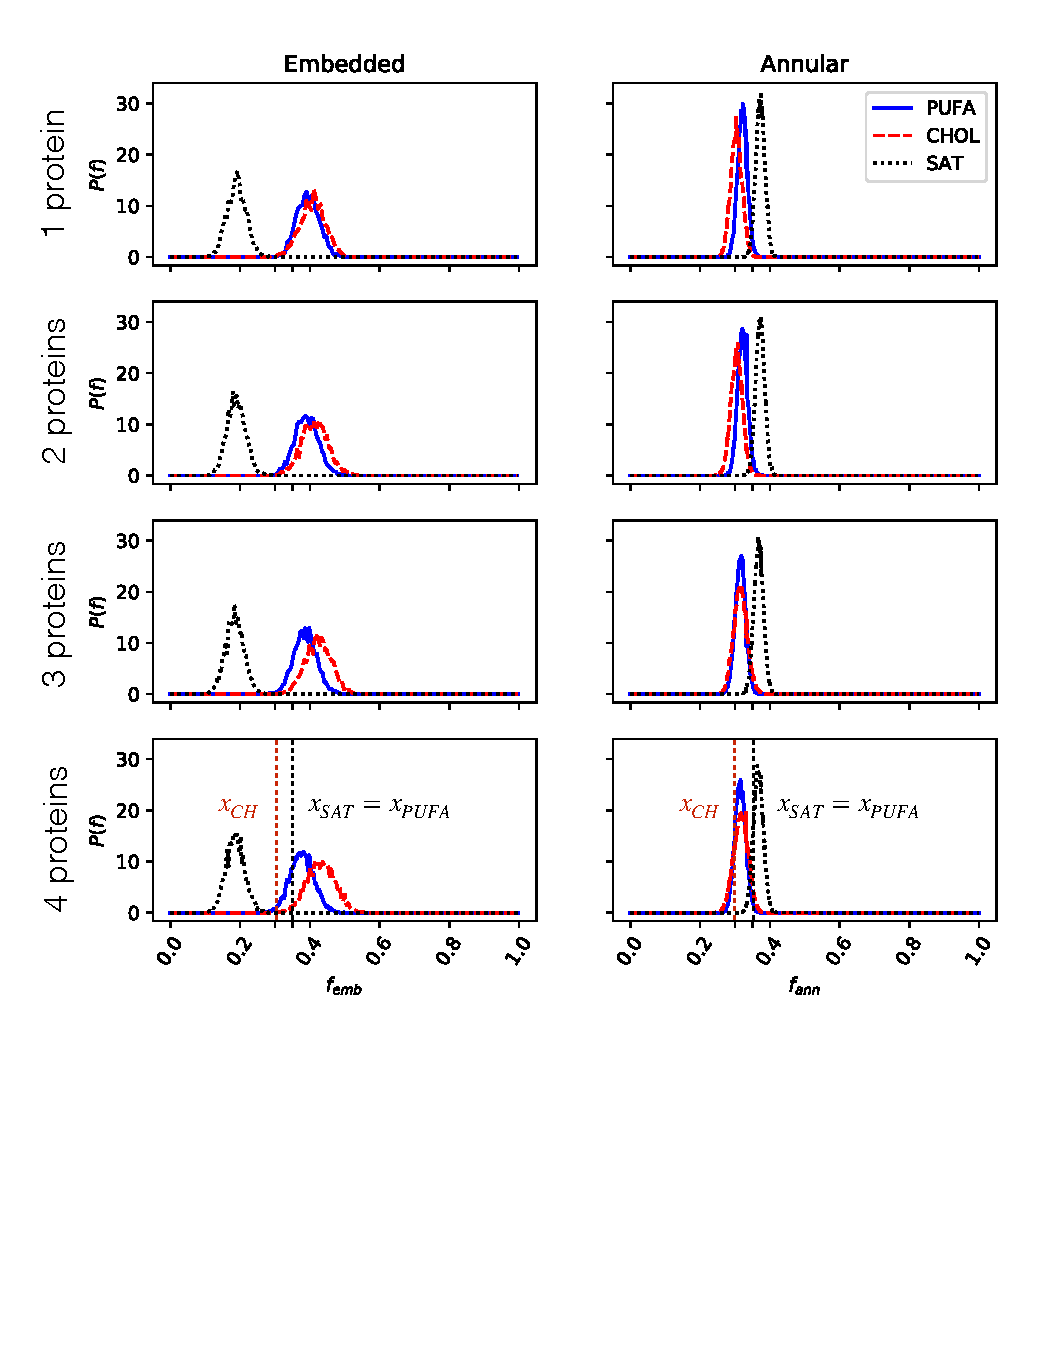
\includegraphics[width=\textwidth]{figure/figure3.pdf}
\caption[Distribution of nAChR boundary cholesterol or acyl chain fractions in mixed membranes containing homoacidic phospholipids.] {Distribution of nAChR boundary cholesterol or acyl chain fractions in mixed membranes containing homoacidic phospholipids. Probability density distribution of fraction of embedded ($f_{emb}$) or annular lipids ($f_{ann}$) as defined in Eq. \ref{eq:f} are shown for 1 to 4 proteins.  Dashed lines represent expected boundary ratios for a randomly-mixed membrane, based on bulk lipid composition ($x_{CH} = 0.3$, $x_{SAT}=x_{PUFA}= 0.35$).}
  \label{fig:Fig2a}
\end{figure}

\begin{figure}[htp]
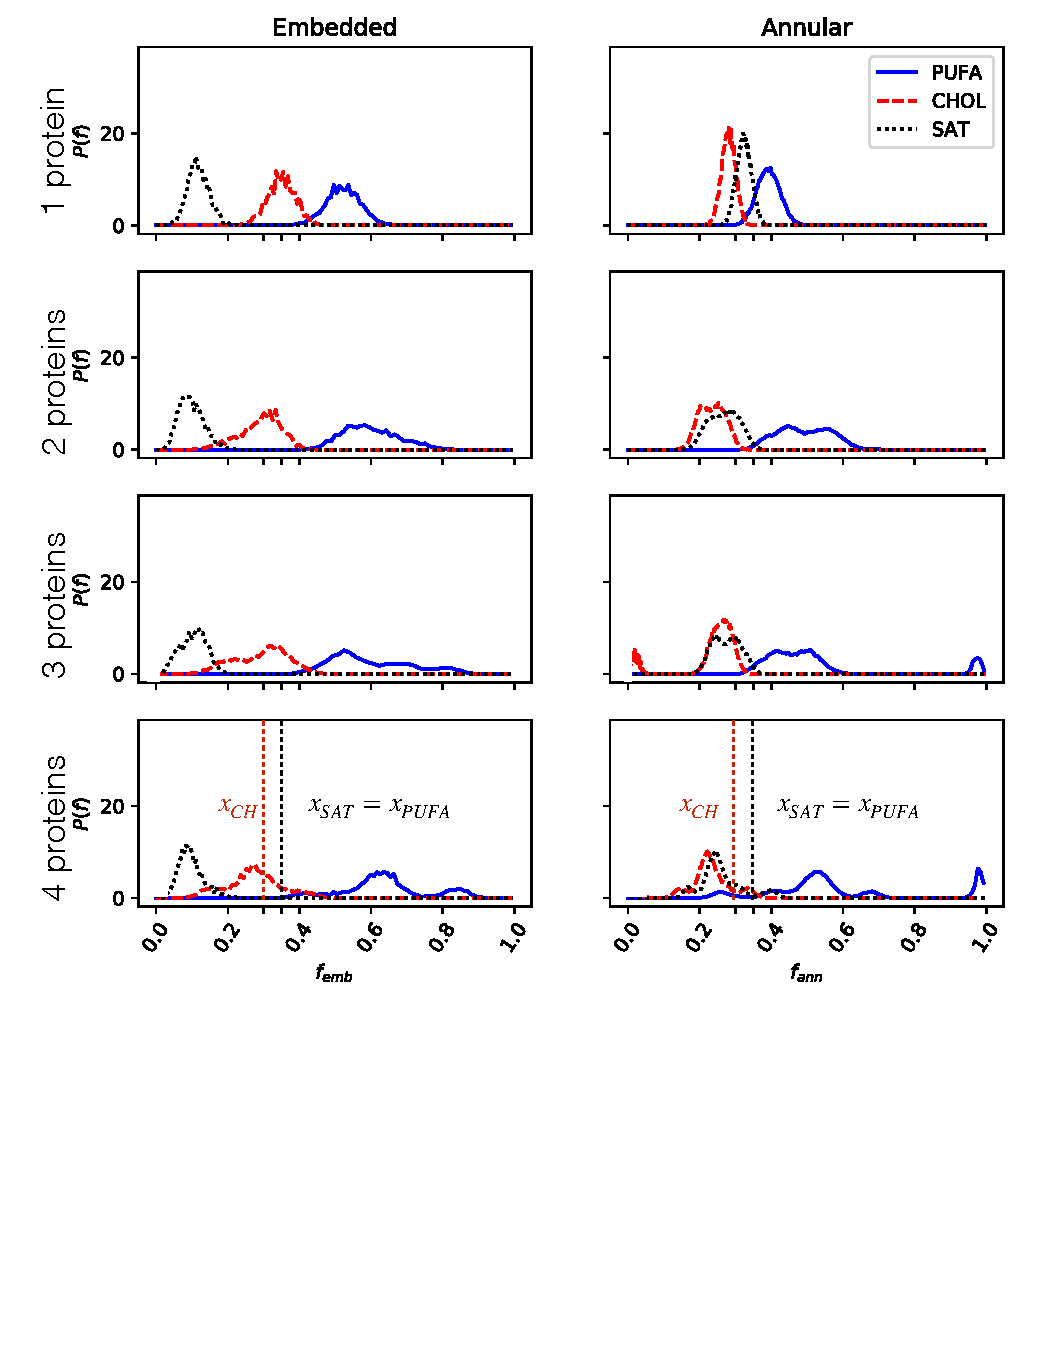
\includegraphics[width=\textwidth]{figure/figure4.pdf}
\caption[Distribution of nAChR boundary cholesterol or acyl chain fractions in mixed membranes containing heteroacidic phospholipids.] {Distribution of nAChR boundary cholesterol or acyl chain fractions in mixed membranes containing heteroacidic phospholipids. Probability density distribution of fraction of embedded ($f_{emb}$) or annular lipids ($f_{ann}$) as defined in Eq. \ref{eq:f} are shown for 1 to 4 proteins.  Dashed lines represent expected boundary ratios for a randomly-mixed membrane, based on bulk lipid composition ($x_{CH} = 0.3$, $x_{SAT}=x_{PUFA}= 0.35$).}\label{fig:Fig2b}
\end{figure}


\begin{figure}[htp]
\includegraphics[width=\textwidth]{figure/Figure5.pdf}
\caption[Enrichment or depletion of lipid species surrounding a single nAChR.] {Enrichment or depletion of lipid species surrounding a single nAChR. Heatmaps represent normalized lipid densities ($\tilde{\rho}_{B}(r_i,\theta_j)$) as defined in Eq. \ref{eq:Rt}, on a scale of -3 (blue, indicating depletion) to 1 (red, indicating enrichment). Densities were averaged over the last 8 $\mu s$ of the 10 $\mu s$ simulations and across three replicas.}
\label{fig:Fig2c}
\end{figure}


The two dimensional density distribution of each lipid species from the center of a single nAChR is shown in Figure \ref{fig:Fig2c}. For all three lipids, there was a five-fold symmetry of densities surrounding nAChR, with lipid preferences determined by transmembrane helix, rather than by subunit. In heteroacid mixtures, cholesterol is enriched near the subunit interfaces, and even buried more deeply within the $\gamma/\alpha$ interface, with saturated acyl chains packed just outside cholesterol.  The outermost M4 helices, however, were packed with PUFAs; PUFA chains also diffused throughout the TMD bundle.  In homoacid membranes, saturated lipids and cholesterol were depleted among embedded lipids, but they maintained the same helix association observed in heteroacid membranes. PUFAs were especially enriched in domain-forming membranes, with high densities around all four transmembrane helices. 

%Next, using Equation \ref{eq:Embedded}, we calculated the average density of each lipid species within 5~nm from the center of nAChR; these data represented the average non-annular lipid concentrations buried within the transmembrane bundle. In Figure \ref{fig:Figure3}, we plotted densities based on headgroup, given that both compositions have idenitical headgroup concentrations (30:PC, 30:PE, 30:CHOL, 10:PS). All data were normalized to account for differences in headgroup concentrations, as well as membrane thicknesses.


%In both domain-forming and hybrid membrane compositions, PS (blue) and PE (magenta) phospholipids were predominately concentrated near the innermost and outermost transmembrane helices, located respectively  approximately 1 nm and 4 nm from the center of mass of nAChR. However, in domain-forming membranes these lipids exhibited a greater affinity for M2 and M4. Meanwhile, cholesterol occupies only 15 \% of non-annular sites in the presence of domains, and up to 12.5 \% in the absence of domains, as seen in Figure \ref{fig:Figure3}; these values show cholesterol relatively depleted throughout the transmembrane bundle compared to its annular concentration shown in Figure~\ref{fig:Figure2}. Across all systems, PC phospholipids were least likely to embed, with a maximum concentration of 12 \% over the 5 nm range. Please see Figure ~\ref{fig:Figure3} for more information.
%\begin{figure}[H]
%\center
%  \subfigure[Domains]{
%    \includegraphics[width=.8\linewidth]{Figure3a}
%    \label{domains}}
%  \subfigure[No domains]{
%    \includegraphics[width=.8\linewidth]{Figure3b}
%    \label{no domains}}
%\caption[Nonannular lipid-binding.]{{\bf Nonannular binding of lipids based on headgroup.} Lipid densities within 5 nm of the nAChR COM (Top: Domain-forming, Bottom:Hybrid). Lipids were colored by headgroup in both compositions (PC: green, PE: purple: CHOL: red, PS: blue).  All data were normalized to account for differences in headgroup concentrations, as well as membrane thicknesses. }
%\label{fig:Figure3}
%\end{figure}
\subsection{nAChR clustering in the presence and absence of lipid domains} \label{sec:clustering}
Here, we repeatedly observed spontaneous formation of receptor dimers in the simulations containing multiple proteins (Figure \ref{fig:Figure4}). 
To investigate the role of lipid domain formation in driving nAChR oligomerization, we calculated the radial distribution function for the pairwise distances between centers of mass, as shown in Figure \ref{fig:Figure6}. For both heteroacid and homoacid membranes, we observed a peak at $r\sim7.5$~nm, corresponding to dimerization.    The differences in profiles between domain and non-domain forming membranes were primarily quantitative: most significantly, the peak corresponding to dimers was substantially higher for 2 and 3 proteins in homoacids than in heteroacids. For two proteins, the distribution for homoacids was shifted to the left, relative to the distribution for heteroacids, indicating that the peak for dimerization was at a shorter distance in domain-forming membranes. This difference is consistent with results indicating a role for domain formation in aggregation and clustering of nAChRs \citep{Barrantes2007,Oshikawa2003,Pato2008}. The simplest explanation of this difference is the higher effective concentration of proteins when domains are present: all nAChRs are corralled in a single liquid-disordered domain, with approximately half the area of the overall membrane.  

\begin{figure}[htp]
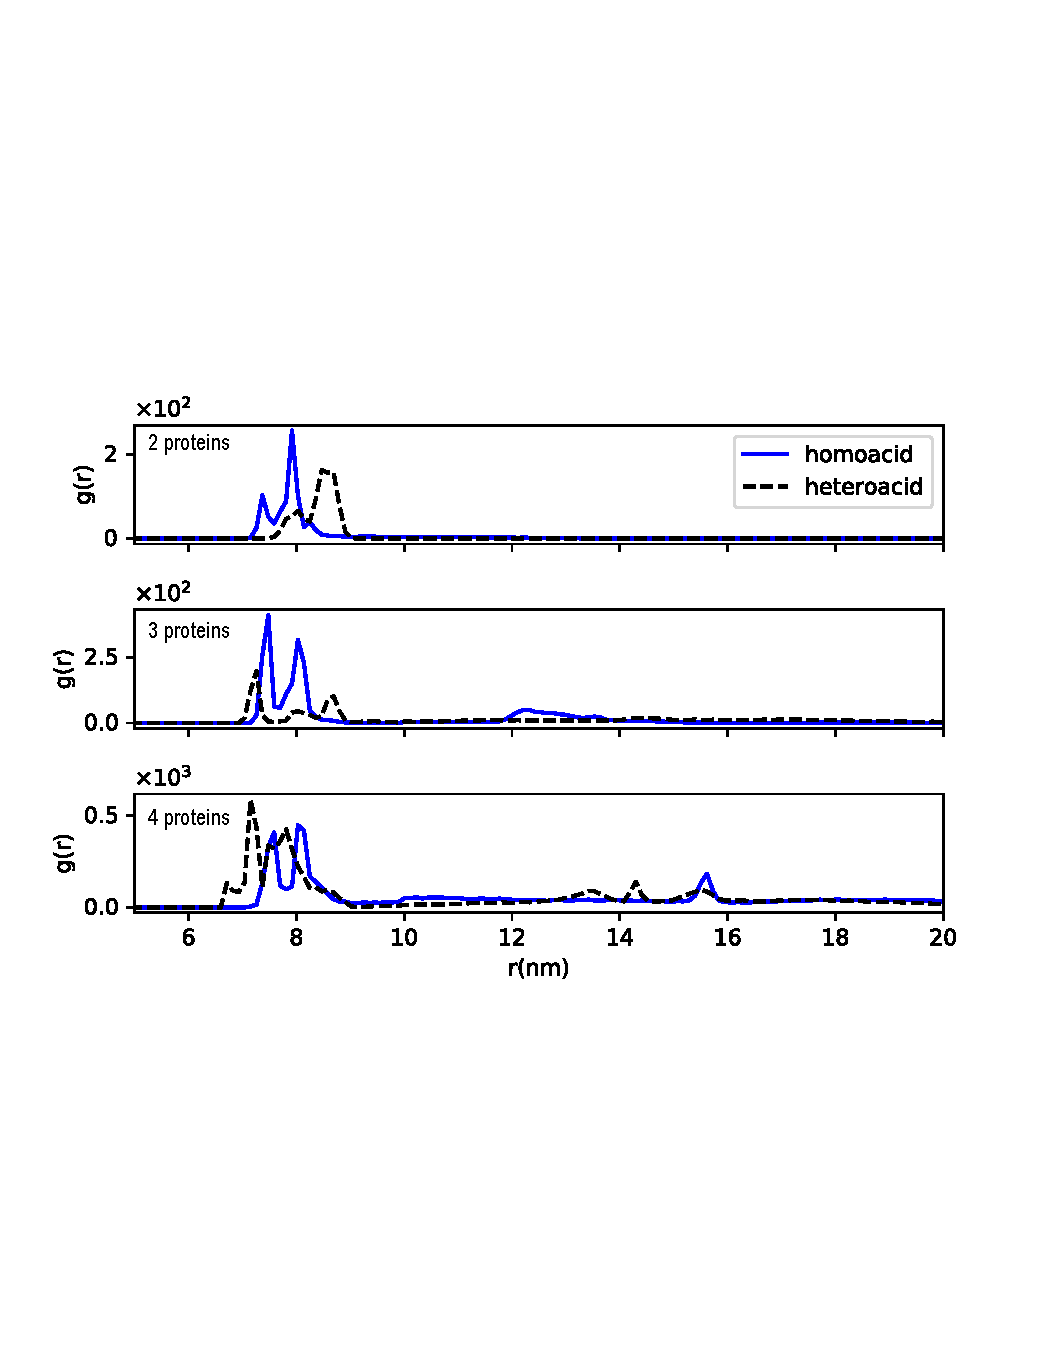
\includegraphics[width=1.0\linewidth]{figure/figure6.pdf}
%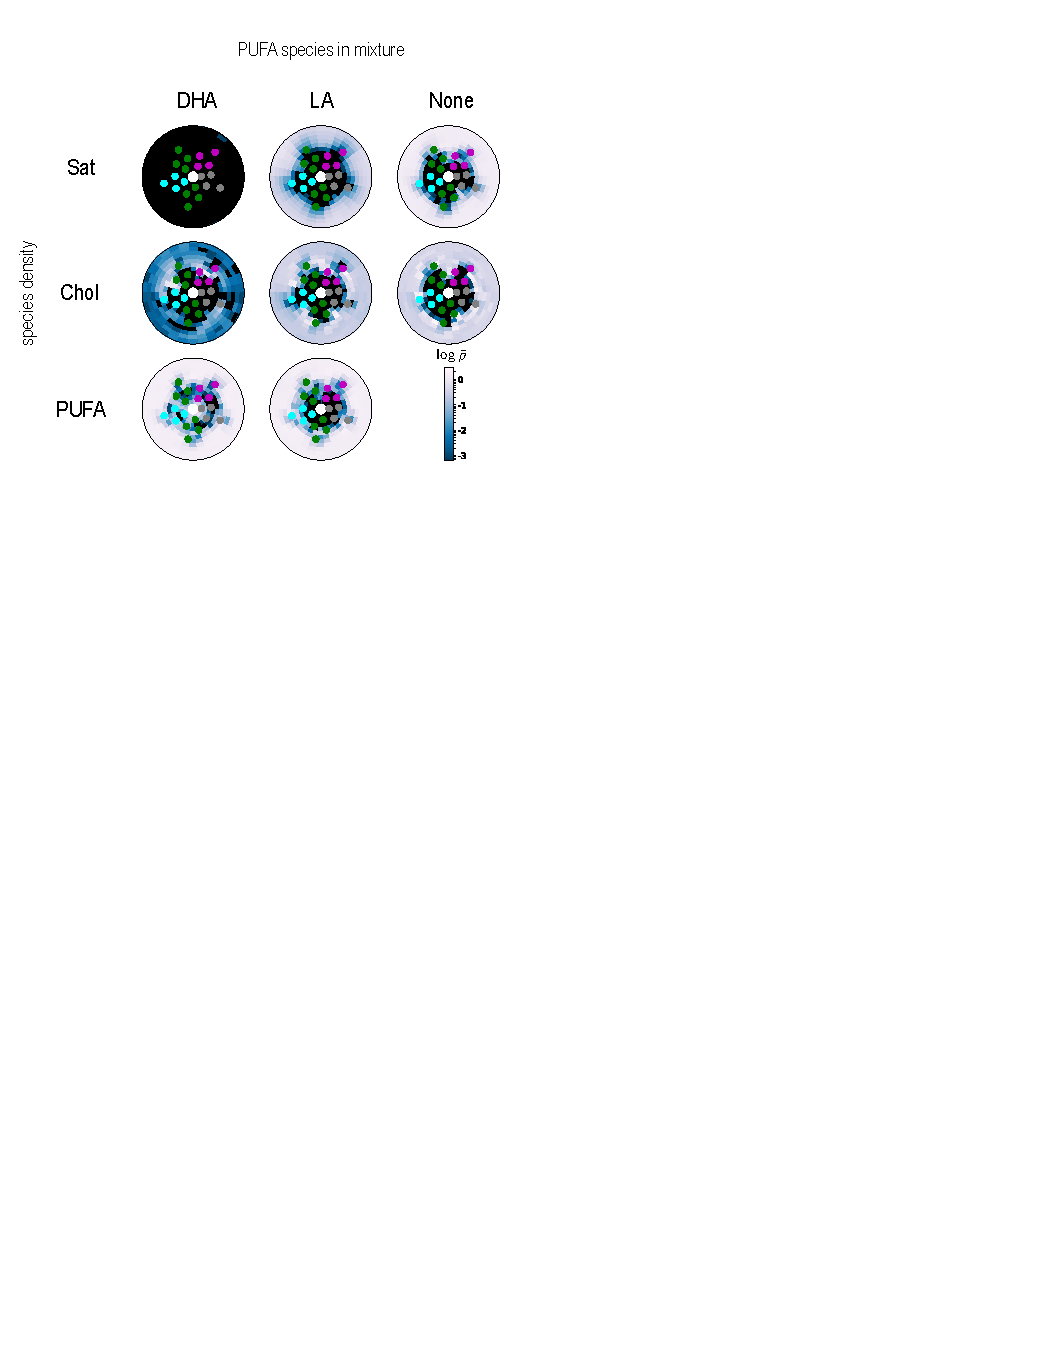
\includegraphics[width=\linewidth,trim={0cm 0cm 0cm 0cm}]{Fig3}
\caption[Pairwise distance distribution across multi-protein systems.] {Pairwise distance distribution across multi-protein systems. Radial distribution function g(r)  of pairwise protein center-of-mass distances, across multi-protein systems. Data collection began at 2 $\mu s$ into each trajectory and ended at 10 $\mu s$, respectively. The peak between 7-10 nm corresponds to dimer formation.}
\label{fig:Figure6}
\end{figure}

%In Figure ~\ref{fig:Figure5}, three subplots depict the average distance between pairs of distinct proteins, in systems containing two, three, or four nAChRs. Across 1500-4000 ns trajectories, the average distance between distinct pairs of proteins is smaller in membranes with well-defined domains, compared to those lacking domains. 

%In the majority of domain-forming membranes, twe observed the formation of nAChR dimers along domain interfaces. Along domains, a majority of pairwise distances  fell within 100-150 {\AA} by 3000 ns (see Figure \ref{fig:Figure4}). This trend persisted within and across individual simulations, regardless of protein concentration or the size and shape of domains.

%\begin{figure}[H]
%	\center
%	\includegraphics[width=\linewidth]{Figure5}
%\caption[Average pairwise distance between nAChR molecules over time.] {{\bf Average pairwise distance between nAChR molecules over time.} Pairwise distance vs time for 12 multi-protein systems.  Here pairwise distance is the average distance between the centers of mass across pairs of proteins.}
%\label{fig:Figure5}
%\end{figure}


\subsection{Closest subunits across dimerizing proteins}
In order to determine whether nAChR dimers were more likely to form with specific subunit interactions, we determined the closest interacting subunit pair for nAChR dimers within each frame. To ensure that dimers, rather than larger oligomers, were being analyzed, we excluded trimers and tetramers from the analysis and only considered two protein systems, with increased sampling. Figure ~\ref{fig:Figure7} shows the amount of enrichment for each possible subunit pairing, relative to an expected random distribution. Results were very sensitive to the use of domain-forming compositions. In heteroacidic membranes, the $\alpha_{\delta}$ subunit formed a monomer-monomer interaction with the $\beta$ subunit, while the $\alpha_{\gamma}$ most favorably interacted with the $\delta$ subunit. In domain-forming membranes,  the $\delta-\alpha_{\delta}-\gamma$ interface was two to five times as likely to pair with a $\alpha_{\delta}$ subunit compared to a random distribution, but substantially more dispersion was detected than in non-domain forming membranes. This difference suggests that nAChRs have preferred dimerization orientations, but membrane organization can reorient receptors. Although $\delta$ subunits are linked by a disulfide bond at the NMJ \citep{Chang1977}, our simulations suggest that without this link, $\delta$ subunits do not form the closest pair among dimerizing proteins.

%{If we do not use three and four protein systems in figure 7, would it be appropriate to discuss possible subunit-subunit pairing for greater number of proteins? Looking at the current plots, I am ''expecting'' if we added more proteins, they would begin to pair off along the white blocks.. }
%Liam, I commented out your remark because GB already addressed it on paper.
%     formation  dependent on  the nAChR $\alpha_{\delta}$ subunit most frequently formed the closest pair, pairing with $\delta$, and $\gamma$ subunits well above expectation (10-15 \%) in both domain-forming and hybrid membranes. In domain-forming membranes, the most frequent closest subunit pairs were $(\alpha_\delta, \delta)$ and $(\alpha_\delta, \gamma)$, each appearing in more than 15 \% of simulations. In hybrid membranes, in addition to the $\alpha_{\delta}$ subunits mentioned above, $(\alpha_\gamma, \gamma)$ were among the closest subunits at a level above expectation. On the other hand, the nAChR $\beta$ subunits formed the fewest subunit pairs, falling well below the expectation value for each pair. Please refer to Figure ~\ref{fig:Figure7} for a heat-map of these data.   



\begin{figure}[htp]
\center{
	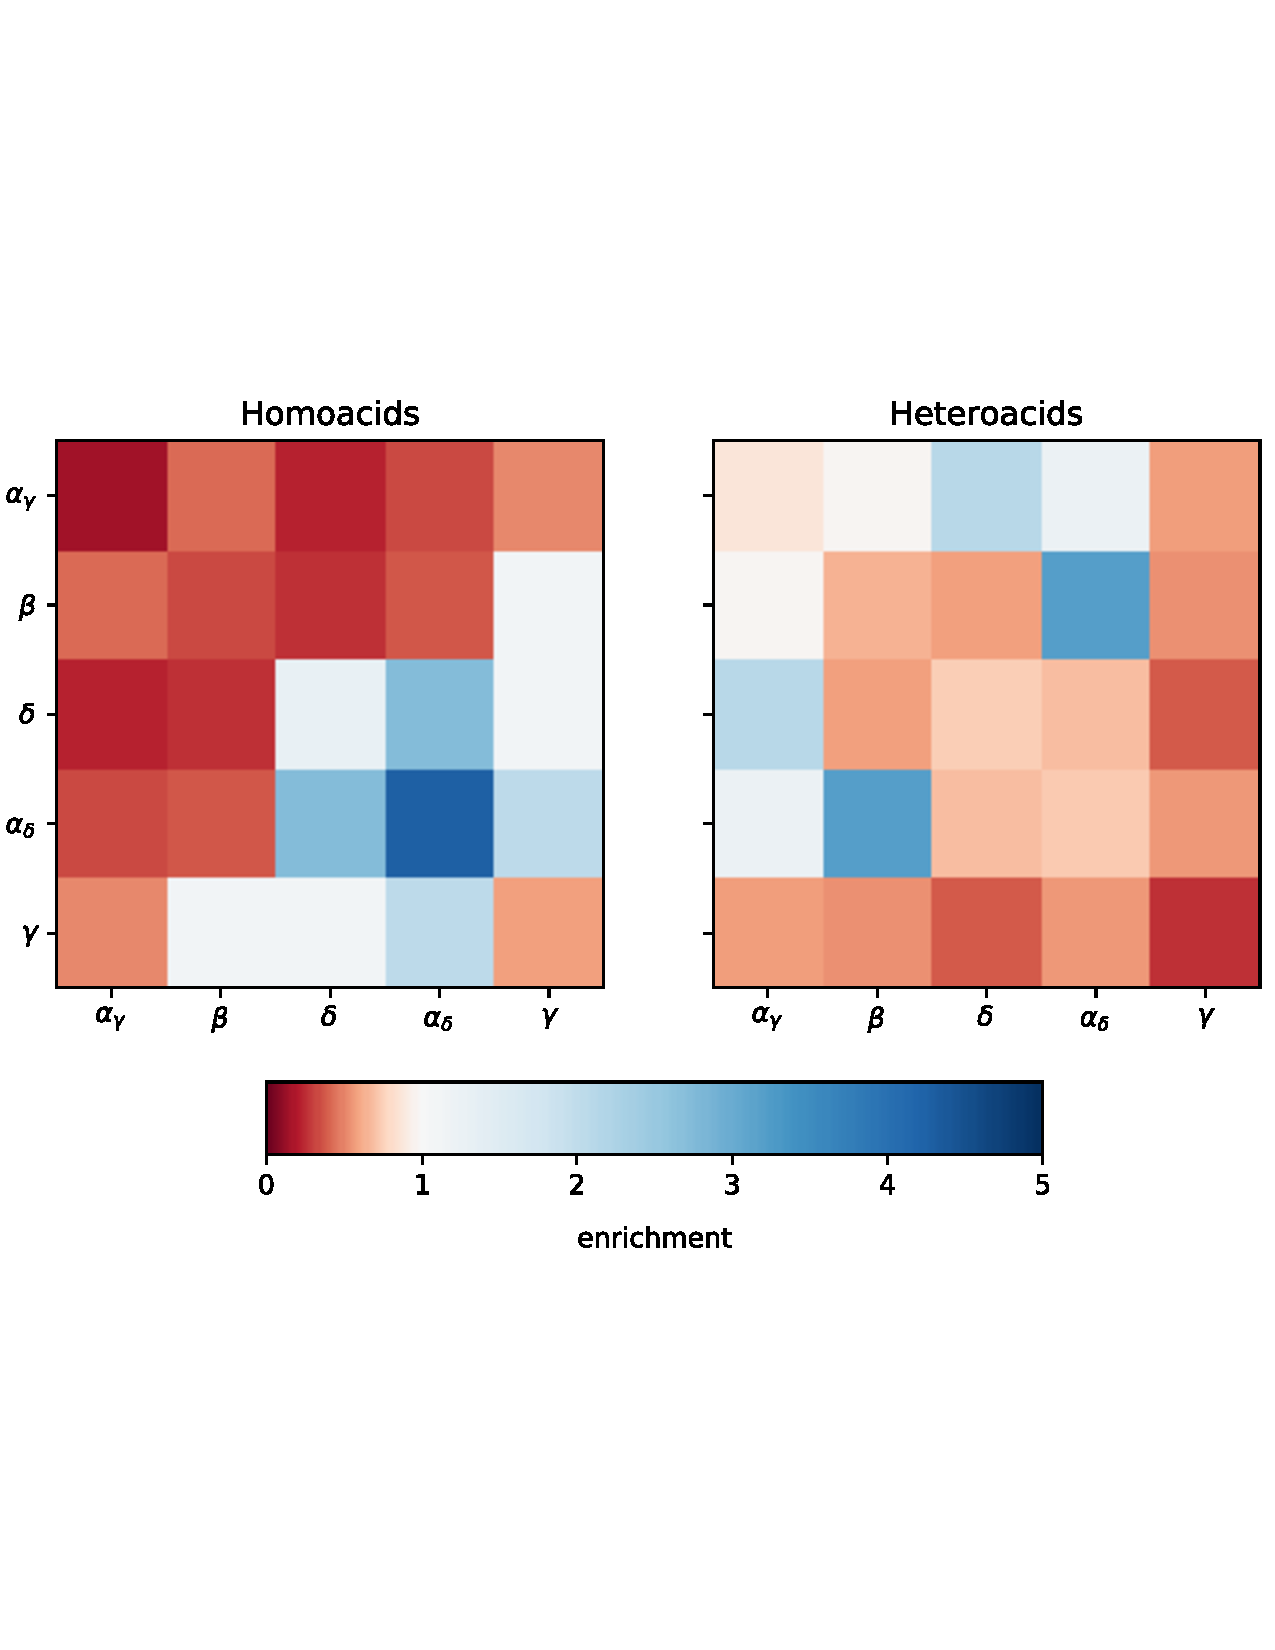
\includegraphics[height=3in]{figure/figure7}}
\begin{flushleft}
\caption[Subunit pairs among dimerizing proteins.] {Subunit pairs among dimerizing proteins. Most probable subunit pairs among dimerizing proteins. Heat-map showing the likelihood that two subunits were closest together among dimerizing proteins (100 {\AA} threshold). Distinct subunits are each expected to form the closest pair 8 \% of the time, while identical subunits are each expected to dimerize only 4 \% of the time. Each color on the heatmap represents multiplicative depletion or enrichment relative to the pair's expectation value, ranging from complete depletion (red) to no enrichment (white) to five-fold enrichment (blue).} 
\end{flushleft}

\label{fig:Figure7}
\end{figure}

\section{Discussion} 

The nAChR is one of the most well-studied, fundamental pLGICs for understanding human cognition, memory, and muscle contraction \citep{Gotti1997}. As an integral membrane protein, the function and organization of nAChR is strongly dictated by its surrounding lipid environment. DHA is an $\omega$-3 polyunsaturated fatty acid abundant in synaptic membranes and the Torpedo electric organs, which are both native nAChR membranes. With its six double bonds, DHA is considered highly disordered and can induce domain formation in membranes \citep{S000930840800032720080101}. We previously observed \citep{Sharp2019} favorable interactions between a single nAChR and DHA-rich, cholesterol-poor domains using coarse-grained simulations. Here, we have extended this approach to investigate the role of lipid topology and domain-formation on boundary lipids of individual nAChRs. We have also conducted the first simulations containing multiple nAChRs, which has allowed us to observe spontaneous dimerization.  

While DHA is implicated in human health and disease, \citep{12439486320170901} experimental studies considering its interactions with nAChR have exclusively considered its free-fatty acid form (FFA), \citep{Antollini2016} %https://www.frontiersin.org/articles/10.3389/fphys.2016.00573/full#h3
rather than as an acyl chain component of a phospholipid. Application of $\omega-3$ FFAs causes a significant reduction in open times observed through single-channel recordings  \citep{Bouzat1993}. Here, we observe a substantial effect of lipid topology on both embedded and annular lipids: DHA chains in homoacidic phospholipids are far more likely to be found as either annular or embedded boundary lipids.  We previously observed only quantitative effects of swapping PE with PC on partitioning, but the headgroup does serve to anchor the lipid at the membrane/protein interface  \citep{Sharp2019}.  DHA in its FFA form (without a headgroup) may diffuse into an open nAChR pore, blocking the channel. %https://www.ncbi.nlm.nih.gov/pubmed?Db=pubmed&Cmd=ShowDetailView&TermToSearch=7522903

We find that, consistent with coarse-grained MD simulations using one nAChR \citep{Sharp2019}, multiple nAChRs continue to prefer the liquid-disordered phase containing long-chain $\omega$-3 fatty acids. While the number of nAChRs in the system did not affect the partitioning profile in these simulations, it did affect the composition of embedded lipids. Our results are consistent with each nAChR monomer in an oligomer blocking access to embedded lipid binding sites in the other monomers, suggesting an intriguing coupling between specific binding and membrane organization.  

Interestingly, upon removing membrane organization, embedded lipids cluster around specific transmembrane helices in a five-fold symmetry around nAChR. This finding suggests that intrinsic lipid preferences are primarily helix dependent, rather than subunit dependent. In homoacid membranes, a lipid preference for DHA was observed across all transmembrane helices, with shells of PUFAs found even at the border of the liquid-ordered phase. Although saturated acyl chains and cholesterol were generally depleted around nAChR, the highest densities for both lipids were found around the M1 and M3 helices, as seen in heteroacid membranes.

In native membranes, nAChR dimers can be stabilized by a disulfide bond between $\delta$ subunits \citep{Chang1977}.  An early controversy \citep{Anholt1980,Ruechel1981,Zingsheim1982,Schindler1984} concerned whether the disulfide bond was necessary for dimer formation. There is no mechanism for covalent bonds between monomers in these coarse-grained simulations. All dimers were stabilized by non-covalent interactions, consistent with the results of \citep{Ruechel1981,Schindler1984}. We observed far more stable dimers in the homoacid mixtures than the heteroacid mixtures, which would be consistent with high sensitivity to experimental conditions. We did not observe a consistent $\delta-\delta$ preference for interfacing subunits in either homoacid or heteroacid mixtures. Schindler {\it et al} (1984) observed an apparent gain-of-function for single-channels within dimers relative to monomers, regardless of disulfide linking \citep{Schindler1984}, suggesting that lipid modulation of oligomerization could also provide a pathway for modulating single channel function. 
\chapter{Direct binding of phosphatidylglycerol at specific sites modulates desensitization of a ligand-gated ion channel}
Originally published in: eLife, 2019, vol 8, pages 1-23\\ \\
%\section[]{Introduction} 

\plgic s are a family of essential proteins evolved for neuronal function in mammals. \plgic are gated by various neurotransmitters, but are functionally modulated by their boundary lipid composition. The well studied \plgic~\nachr conducts cations across the membrane to stimulate an action potential, and is functionally dependent on cholesterol and anionic lipids \citep{Dalziel1980,Ellena1983,M.CriadoH.Eibl1982,Fong1986,Fong1987,Jones1988a,Sunshine1994,DaCosta2009b}. Lipid binding sites for \plgic s are still relatively unknown.  Structural biology has predicted cholesterol and fatty acid binding sites in \plgic s \citep{Laverty2017,Basak2017}. Coarse grained molecular dynamics (CGMD) work by Sharp\citep{Sharp2019} and Woods\citep{Woods2019} predicted cholesterol binding sites around \nachr. \plgic-anionic lipid binding sites are still unknown. 

This work is the computational portion of a collaborative project analyzing \plgic~Erwinia ligand-gated ion channel's (ELIC) model boundary charged lipid composition using native mass spectrometry (NMS). Using CGMD as a computational microscope and simulating ELIC in membranes comprised of neutral 1-palmitoyl-2-oleoyl-sn-glycero-3-phosphocholine (POPC) and 1-palmitoyl-2-oleoyl-sn-glycero-3-phosphoethanolamine (POPE) and anionic 1-palmitoyl-2-oleoyl-sn-glycero-3-phosphoglycerol (POPG) we visualize and test potential anionic-ELIC binding distributions from NMS studies performed in \citep{Tong2019}. This work sought to determine 1) if charged phospholipids bound to ELIC, 2) determine where they bind, and 3) determine which sites modulate function.

\section[]{Computational Methods}
All simulations reported here used the MARTINI 2.2 \citep{DeJong2012} coarse-grained
topology and force field. The crystal structure of ELIC (PDB 3RQW) \citep{Pan2012}
was coarse-grained using MARTINI martinize.py script. Secondary
structural restraints were constructed using martinize.py while imposed
through Gromacs \citep{Berendsen1995}. Conformational restraints were preserved through
harmonic bonds between backbone beads less than 0.5 nm apart with a
coefficient of 900 kJ mol\textsuperscript{-1}. Pairs were determined
using the ElNeDyn algorithm \citep{Periole2009}. Membranes were constructed using the
MARTINI script insane.py \citep{Wassenaar2015}. The insane.py script randomly places
lipids throughout both inner and outer membranes and embeds selected
proteins into the membrane. Two series of simulations were developed,
the first using POPE and POPG, and the second POPC and POPG. Box sizes
were about 30 x 30 x 25 nm\textsuperscript{3} and each simulation box
contained about 3000 lipids.

Molecular dynamics simulations were carried out using GROMACS 5.1.4
\citep{Berendsen1995}. All systems were run using van der Waals (vdW) and electrostatics
in cutoff and reaction-field, respectively, with a dielectric constant
of $\epsilon = 15$. vdW and electrostatics used a cutoff length of
1.1 nm as defined in current MARTINI build specifications. Energy
minimizations were performed for about 30,000 steps. All systems were
run for short equilibration steps. Canonical ensembles (NVT) were run
for 100 ps using Berendsen thermostat set to 323 K with the temperature
coupling constant set to 1 ps. Isothermal-Isobaric ensemble (NPT)
equilibration was run for 5000 ps using Berendsen thermostat and
barostat. The thermostat was set to 323 K with the temperature coupling
constant set to 1 ps, and the barostat was set to a pressure coupling
constant of 3 ps with a compressibility of $3 x 10^{-5}$
bar$^{-1}$ holding at 1 bar. Molecular dynamics were
carried out using NPT ensemble and were simulated for 15 $\mu$s with a time
step of 0.015 ps using v-rescale thermostat set to 323 K and a
temperature coupling constant of 1 ps. Membranes consisting of POPE used
the Parrinello-Rahman barostat, and membranes consisting of POPC used
the Berendsen barostat, both under semi-isotropic coupling. The
reference pressure was set to 1 bar, the compressibility
3x10$^{-4}$ bar$^{-1}$, and the pressure
coupling constant 1 ps.

Annular lipids were determined using the annular lipid metric B:
\begin{equation}
    \begin{aligned}
    B_{i} = \left\langle \frac{b_{i}}{b_{\text{tot}}} \right\rangle\frac{1}{x_{i}} - 1
    \label{eq:B}
    \end{aligned}
\end{equation}

where $b_{i}$ is the instantaneous number of boundary lipids of
species $i$, $b_{\text{tot}}$ is the instantaneous total number of
boundary lipids, $x_{i}$ is the overall (bulk) fraction of species
$i$ and the brackets represent an average over time and replicas.
$B_{i} < 0$ and $B_{i} > 0$ indicate
enrichment and depletion of species $i$, respectively, relative to the
abundance in the bulk membrane. A given lipid was counted as a boundary
lipid if it was within 6 \AA of the ELIC transmembrane domain.

Two dimensional lipid density distributions around a central ELIC
pentamer were calculated for each leaflet using polar coordinates \citep{Sharp2019}.
For every sampled frame, all lipids of species $i$ were separated into
leaflets. For all $i$ lipids in a given leaflet, the vector separating
the phosphate beads from ELIC center was calculated and projected onto
the membrane plane. The two-dimensional separation vector was then used
to assign the lipid to the appropriate polar bin of radial bin width
$4\AA$ and angular bin width
$\frac{\pi}{15}$. The area density in each bin was averaged
over time and replicas.

\section[]{Computational Results}

To examine phospholipid interactions with ELIC using a molecular
model, coarse-grained MD simulations were performed on binary POPG/POPC
and POPG/POPE model membranes containing a single ELIC pentamer (Fig.
\ref{fig:Elic1}). Unlike fully-atomistic simulations, coarse-grained simulations
permit significant diffusion of lipids over simulation time scales. The
boundary lipid composition can thus equilibrate over the simulation
time, even if it varies significantly from the bulk membrane
composition. The POPG fraction was varied between 0 and 70\%. Enrichment
or depletion of POPG among boundary lipids for each concentration was
quantified using the boundary lipid metric B (Equation 3, see Methods).
For a given lipid species, $B>0$ reflects enrichment, $B<0$ reflects depletion, and B=0 reflects random mixing. For
POPG,$B>0$ for all compositions tested (Fig. \ref{fig:Elic1}B). This
result indicates that if POPG is present in the membrane, it is enriched
among boundary lipids. This enrichment is strongest for lower amounts of
POPG (i.e. lower $x_{\text{POPG}}$), consistent with specific binding
of POPG to ELIC.

\begin{figure}[htp]
	\center
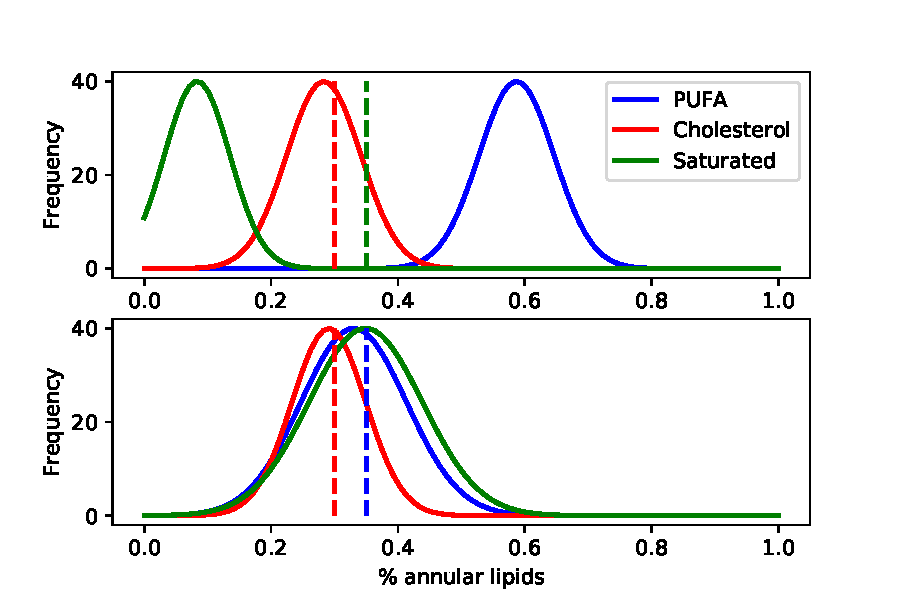
\includegraphics[width=.5\linewidth]{ELIC/Figure1.pdf}
\caption{Enrichment of POPG among ELIC boundary phospholipids from coarse-grained simulations. (A) Image of the simulation model of ELIC embedded in a membrane consisting of 10$\%$ POPG (pink) and $\%$ POPC (blue). The view is from the extracellular side of ELIC perpendicular to the membrane. (B) The boundary enrichment metric, B, is shown for phospholipid species in POPC/POPG membranes (left) or POPE/POPG membranes (right) over a range of POPG mole fractions $(x_PG)$. B is defined in Equation 3 (see Methods) and reflects the fractional difference between the amount of a lipid species found in the boundary and the bulk membrane: $B>0$ indicates enrichment, B<0 indicates depletion, and $B = 0$ indicates no difference in mole fraction between the bulk and the boundary. }
\label{fig:Elic1}
\end{figure}

We further examined these sites of interaction using our coarse-grained
MD simulations. To identify whether boundary POPG were localized around
specific helices or residues, two-dimensional densities of the
negatively-charged headgroup bead were calculated. The distributions are
separated by leaflet where each leaflet contained 10\% POPG. As shown in
Figure 5A, POPG was more likely to interact with ELIC in the inner
leaflet than the outer leaflet, consistent with three out of five
interfacial arginines residues being located on the intracellular
interface of the ELIC TMD. These three arginines are located on TM3
(R286) and TM4 (R299 and R301). Contacts between POPG and all three of
these residues are also visible in individual frames of the simulation
(Fig. 5B). Moreover, POPG is more likely to be contacting the
interfacial residues in TM4 (such as R299 and R301) than accessible
interfacial residues in any other helices (Fig. \ref{fig:Elic2}A). The remaining two
arginine residues are located at the TMD-ECD interface (R117 and R123).
POPG density in the outer leaflet localized to these residues at
intrasubunit sites between TM4 and TM1 or TM4 and TM3 (Fig. \ref{fig:Elic2}A), and
contacts between these residues and POPG headgroups in the outer leaflet
were also observed in snapshots from the MD simulations (Fig. \ref{fig:Elic2}B). In
summary, the native MS data and coarse-grained MD simulations
demonstrate that five interfacial arginines contribute to specific POPG
binding sites in the inner and outer leaflets adjacent to TM4.

\begin{figure}[htp]
	\center
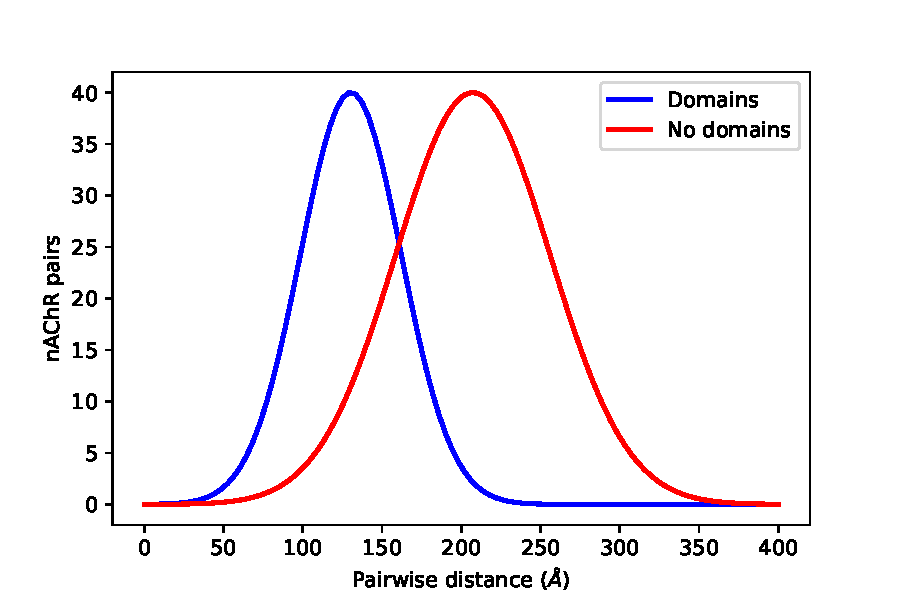
\includegraphics[width=\linewidth]{ELIC/Figure2.pdf}. 
\caption{Density calculations of lipids in binary membranes and visualization of direct POPG-ELIC interactions at $10\%$ POPG. (A) Distribution of POPG density in a POPG-POPC membrane, within 40 \AA from the ELIC pore over the last half of a 15 $\mu$s simulation, for both the outer leaflet (top) and the inner leaflet (bottom). Density is colored according to the color bar, where red and blue represent low and high POPG density, respectively. Circles represent the ELIC transmembrane backbone center of mass, with the helices containing the interfacial arginines colored in red (B) Representative frames after ~9 $\mu$s of simulation, showing multiple POPG binding modes associated with high density areas in (A). Two adjacent subunits of ELIC are shown in grey and white, while arginine side chains of interest are colored in peach, lime-yellow, orange, yellow, and red. POPG phosphate is colored in tan with the rest of the lipid in cyan.}
\label{fig:Elic2}
\end{figure}

\section[]{Summary}

This work sought to determine 1) if charged phospholipids bound to ELIC, 2) determine where they bind, and 3) determine which sites modulate function. NMS showed of the lipids POPC, POPE, and POPG, POPG consistently bound to ELIC more than either neutral lipid. Using CGMD we calculated the boundary enrichment of POPC, POPE, and POPG. We found POPG had the highest enrichment at the lowest concentration. This suggests specific binding sites for anionic lipids. Arginine residues at around the  TMD interfaces were hypothesized to be potential PG binding sites. Mutational studies, replacing positive arginine with polary neutral glutamine, in conjunction with NMS and electrophysiology, showed 1) less POPG bound and 2) a loss of function. CGMD density calculations predicted locations of high POPG density around inner intersubunit sites around ELIC's TMD. Each site contain 3 arginine. This suggests 1) anionic lipids bind to intersubunit sites, where positively charged arginine is, 2) mutating arginine to a polar neutral amino acid reduces anionic lipid binding, and 3) ELIC is functionally dependent on these arginines.

%\includepdf[pages={1-23},scale=1]{./ELIC/Tong2019}
%\documentclass[]{article}
%\usepackage{lmodern}
%\usepackage{amssymb,amsmath}
%\usepackage{ifxetex,ifluatex}
%\usepackage{fixltx2e} % provides \textsubscript
%\ifnum 0\ifxetex 1\fi\ifluatex 1\fi=0 % if pdftex
%  \usepackage[T1]{fontenc}
%  \usepackage[utf8]{inputenc}
%\else % if luatex or xelatex
%  \ifxetex
%    \usepackage{mathspec}
%  \else
%    \usepackage{fontspec}
%  \fi
%  \defaultfontfeatures{Ligatures=TeX,Scale=MatchLowercase}
%\fi
%% use upquote if available, for straight quotes in verbatim environments
%\IfFileExists{upquote.sty}{\usepackage{upquote}}{}
%% use microtype if available
%\IfFileExists{microtype.sty}{%
%\usepackage[]{microtype}
%\UseMicrotypeSet[protrusion]{basicmath} % disable protrusion for tt fonts
%}{}
%\PassOptionsToPackage{hyphens}{url} % url is loaded by hyperref
%\usepackage[unicode=true]{hyperref}
%\hypersetup{
%            pdfborder={0 0 0},
%            breaklinks=true}
%\urlstyle{same}  % don't use monospace font for urls
%\usepackage{longtable,booktabs}
%% Fix footnotes in tables (requires footnote package)
%\IfFileExists{footnote.sty}{\usepackage{footnote}\makesavenoteenv{long table}}{}
%\usepackage{graphicx,grffile}
%\makeatletter
%\def\maxwidth{\ifdim\Gin@nat@width>\linewidth\linewidth\else\Gin@nat@width\fi}
%\def\maxheight{\ifdim\Gin@nat@height>\textheight\textheight\else\Gin@nat@height\fi}
%\makeatother
%% Scale images if necessary, so that they will not overflow the page
%% margins by default, and it is still possible to overwrite the defaults
%% using explicit options in \includegraphics[width, height, ...]{}
%\setkeys{Gin}{width=\maxwidth,height=\maxheight,keepaspectratio}
%\IfFileExists{parskip.sty}{%
%\usepackage{parskip}
%}{% else
%\setlength{\parindent}{0pt}
%\setlength{\parskip}{6pt plus 2pt minus 1pt}
%}
%\setlength{\emergencystretch}{3em}  % prevent overfull lines
%\providecommand{\tightlist}{%
%  \setlength{\itemsep}{0pt}\setlength{\parskip}{0pt}}
%\setcounter{secnumdepth}{0}
%% Redefines (sub)paragraphs to behave more like sections
%\ifx\paragraph\undefined\else
%\let\oldparagraph\paragraph
%\renewcommand{\paragraph}[1]{\oldparagraph{#1}\mbox{}}
%\fi
%\ifx\subparagraph\undefined\else
%\let\oldsubparagraph\subparagraph
%\renewcommand{\subparagraph}[1]{\oldsubparagraph{#1}\mbox{}}
%\fi
%
%% set default figure placement to htbp
%\makeatletter
%\def\fps@figure{htbp}
%\makeatother
%
%
%\date{}
%
%\begin{document}
Ailing Tong\textsuperscript{1}, John T. Petroff II\textsuperscript{1},
Fong-Fu Hsu\textsuperscript{2}, Philipp A. M.
Schmidpeter\textsuperscript{3}, Crina M. Nimigean\textsuperscript{3},
Liam Sharp\textsuperscript{4}, Grace Brannigan\textsuperscript{4,5},
Wayland W. L. Cheng\textsuperscript{1,}*

From the Departments of \textsuperscript{1}Anesthesiology, and
\textsuperscript{2}Internal Medicine, Mass Spectrometry Resource,
Division of Endocrinology, Diabetes, Metabolism, and Lipid Research,
Washington University in St. Louis, MO, USA,
\textsuperscript{3}Departments of Anesthesiology, and Physiology and
Biophysics, Weill Cornell Medicine, NY, USA, and the
\textsuperscript{4}Center for Computational and Integrative Biology and
\textsuperscript{5}Department of Physics, Rutgers University, Camden,
NJ, USA.

*To whom correspondence should be addressed: Professor Wayland W. L.
Cheng, Department of Anesthesiology, Washington University School of
Medicine, Campus Box 8054, St. Louis, MO 63110. Telephone:
(314)273-7958; E-mail: wayland.cheng@wustl.edu

\section{Abstract}

Pentameric ligand-gated ion channels (pLGICs) are essential determinants
of synaptic transmission, and are modulated by specific lipids including
anionic phospholipids. The exact modulatory effect of anionic
phospholipids in pLGICs and the mechanism of this effect are not well
understood. Using native mass spectrometry, coarse-grained molecular
dynamics simulations and functional assays, we show that the anionic
phospholipid, 1-palmitoyl-2-oleoyl-phosphatidylglycerol (POPG),
preferentially binds to and stabilizes the pLGIC, Erwinia ligand-gated
ion channel (ELIC), and decreases ELIC desensitization. Mutations of
five arginines located in the interfacial regions of the transmembrane
domain (TMD) reduce POPG binding, and a subset of these mutations
increase ELIC desensitization. In contrast, the L240A mutant increases
POPG binding and decreases ELIC desensitization. The results support a
mechanism by which POPG stabilizes the open state of ELIC relative to
the desensitized state by direct binding at specific sites.

\section{Introduction}

Pentameric ligand-gated ion channels (pLGICs) are essential determinants
of synaptic transmission, and the targets of many allosteric modulators
including general anesthetics and anti-epileptics (1). These ion
channels are embedded in a heterogeneous and dynamic lipid environment
(2), and the presence of specific lipids fine-tunes the function of
pLGICs and may play a role in regulating neuronal excitability and drug
sensitivity (3-5). One nearly ubiquitous example is that of anionic
phospholipids, which are known to modulate pentameric ligand-gated ion
channels (pLGICs) such as the nicotinic acetylcholine receptor (nAchR)
(6), as well as inward rectifying potassium channels (7), K(2P) channels
(8), voltage-gated potassium channels (9, 10), and cyclic
nucleotide-gated channels (11). In pLGICs, anionic phospholipids have
been shown to shift the conformational equilibrium of the channel from
an uncoupled or desensitized state to a resting state, in which agonist
binding is effectively coupled to channel activation (12-14).

Studies of lipid modulation of ion channel function including modulation
of pLGICs have focused on two central questions: 1) what is the exact
effect of the lipid on channel function and structure, and 2) is the
effect attributable to direct binding of the lipid at specific sites?
\emph{Torpedo} nAchR channel activity measured from flux assays (6, 15,
16) and agonist-induced conformational changes (13, 17) depend on
anionic phospholipids. However, few studies have employed fast solution
changes to measure current responses of pLGICs in model membranes (18),
which is necessary to distinguish the effect of lipids on channel
gating, specifically transitions between resting, open and desensitized
states. With regard to lipid binding, early studies using electron
paramagnetic resonance (EPR) of spin-labeled lipids or lipid-induced
modification of fluorescent probes revealed an immobilized layer of
lipids surrounding nAchRs that is enriched for certain phospholipids
(19, 20) with lipids occupying specific sites (21, 22). These approaches
are, however, an indirect means to examine lipid binding to ion
channels. More recently, crystal structures of the pLGIC, Gloeobacter
ligand-gated ion channel (GLIC), revealed bound, co-purified
phospholipids in a putative open structure, and the absence of one of
these phospholipids in a locally-closed structure (23, 24). Similarly, a
putative desensitized structure of GLIC with a bound polyunsaturated
fatty acid showed loss of the aforementioned phospholipid density that
is bound to the open state (25). Both of these studies suggest that
bound phospholipids at specific sites stabilize the open state of the
channel, although the identity of these lipids remains unknown.
Furthermore, the absence of a lipid density in a crystal structure is
not necessarily an indication of lack of binding.

Native mass spectrometry (MS) has proven to be a powerful tool to
directly measure binding of endogenous and exogenous lipids to membrane
proteins (26, 27), although this approach has yet to be used to examine
pLGIC-lipid interactions. In addition, coarse-grained molecular dynamics
(MD) simulations provide a complementary approach to examine lipid
interactions with membrane-embedded pLGICs at time scales that allow
equilibration of lipid binding sites (28, 29). We sought to determine
whether phospholipids bind directly and selectively to a pLGIC by native
MS and coarse-grained MD simulations, and whether specific binding
interactions modulate channel function by patch-clamp recordings and
stopped-flow ion flux measurements from liposomes of defined lipid
composition. Erwinia ligand-gated ion channel (ELIC), a prototypical
pLGIC and biochemically tractable target, is also sensitive to its lipid
environment. ELIC was found to be inactive when reconstituted in
1-palmitoyl-2-oleoyl-phosphatidylcholine (POPC) membranes fused to
\emph{Xenopus} oocyte membranes, similar to the nAchR (30). After
optimizing native MS for ELIC, we demonstrate that phospholipids
directly bind to ELIC, with more binding observed for the anionic
phospholipid, POPG compared to zwitterionic phospholipids,
1-palmitoyl-2-oleoyl-phosphatidylethanolamine (POPE) and POPC.
Consistent with this finding, coarse-grained simulations of ELIC in a
lipid bilayer show enrichment of annular POPG compared to POPC or POPE
phospholipids. In addition, POPG selectively stabilizes ELIC against
thermal denaturation indicative of a specific binding interaction, and
reduces channel desensitization. Mutations of five arginines at the
transmembrane domain (TMD) intracellular and extracellular interfaces
decrease PG binding while a subset of these mutations increase
desensitization. Likewise, the L240A mutant, which reduces
desensitization, increases PG binding. The results support the
long-standing hypothesis that anionic phospholipids stabilize the open
state of pLGICs by direct binding to sites in the TMD adjacent to the
lipid-facing transmembrane helix 4 (TM4) (3).

\section{Results}

\subsection{Selective binding of phospholipids to ELIC}

\begin{figure}
\center
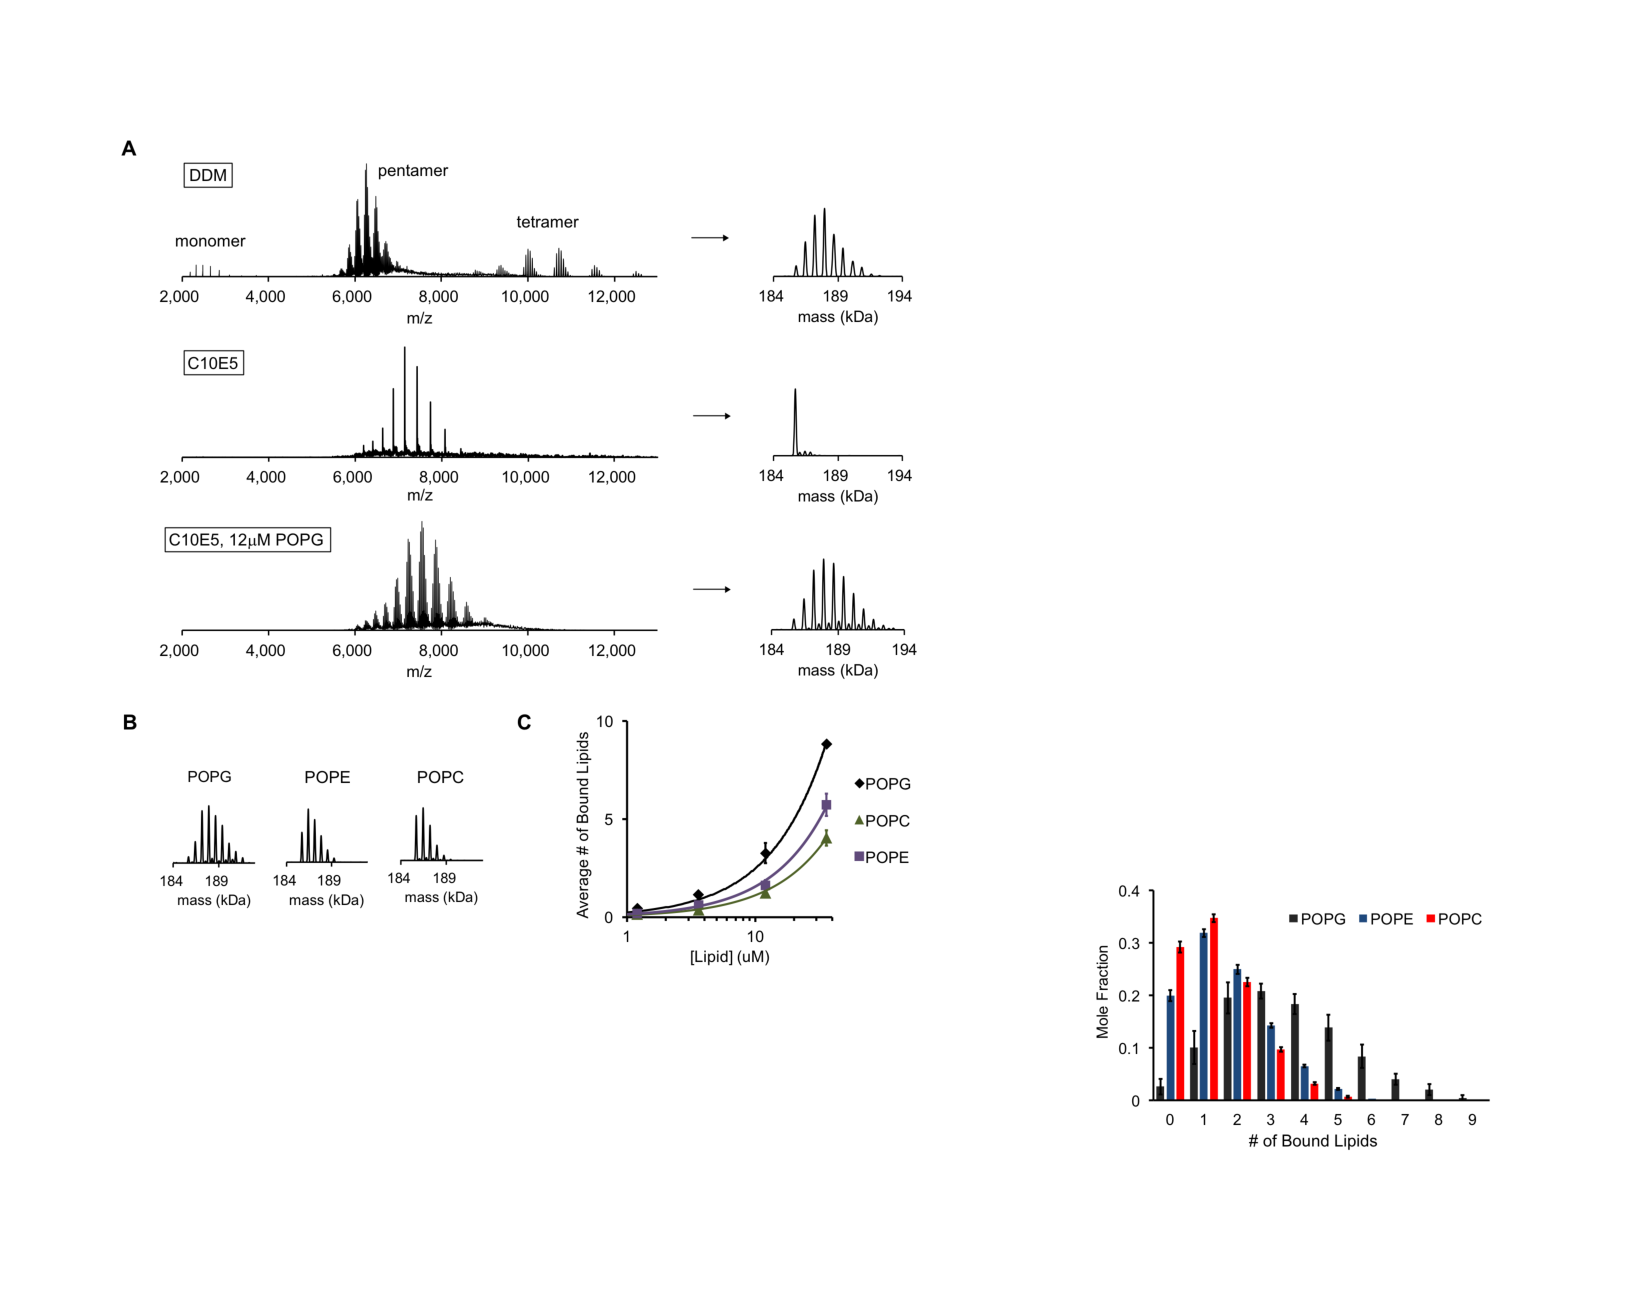
\includegraphics[width=\linewidth]{./pandoc_test/media/image1.pdf}
	\begin{flushleft}

\caption[POPG binds selectively to ELIC.] {POPG binds selectively to ELIC. (A) Native MS spectra of ELIC in DDM, C10E5, and C10E5 with 12 $\mu$M POPG. Left shows full spectra and right shows deconvoluted spectra. (B) Deconvoluted spectra of ELIC in 12 $\mu$M of the indicated phospholipid. (C) Plot of the average number of bound phospholipids per pentamer at varying concentrations of POPG, POPE and POPC (n=3-6, $\pm$SD). Data are fit to a sigmoid binding curve.}
	\label{fig:one}
	\end{flushleft}

\end{figure}

Native MS of ELIC purified in dodecyl maltoside (DDM) was optimized on a
Q-Exactive EMR mass spectrometer as previously described (27). Optimal
desolvation of the pentamer required activation energies that resulted
in some dissociation into tetramer and monomer (Fig. \ref{fig:one}A). Nevertheless,
both the pentamer and tetramer species showed multiple bound small
molecules of \textasciitilde{}750 Da, likely corresponding to
co-purified phospholipids (up to 8 and 6 lipids per multimer were
observed for the pentamer and tetramer, respectively) (Fig. \ref{fig:one}A). To
determine the identity of these lipids, we performed a lipid extraction
from the purified ELIC preparation, and analyzed the sample using tandem
MS. This revealed multiple PE and PG phospholipids with different acyl
chains that mirror the phospholipids extracted from \emph{E. coli}
membranes (Table \ref{tab:Supplementary Table 1}). Quantification of the MS intensities
for PG relative to PE species yielded a higher relative abundance of PG
co-purified with ELIC compared to \emph{E. coli} membranes, suggesting
that ELIC preferentially binds PG in its native environment
(Fig. \ref{fig:Supplementary Fig. 1}, Table \ref{tab:Supplementary Table 1}).

\begin{figure}
\center
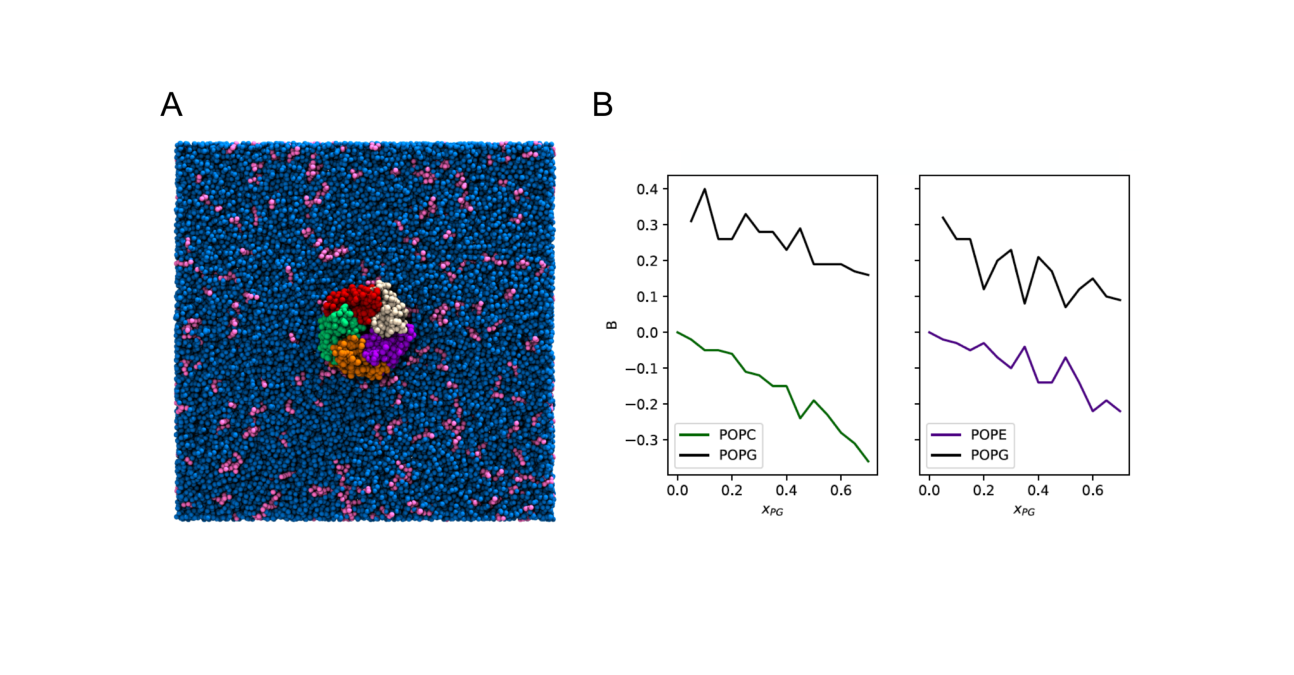
\includegraphics[width=\linewidth]{./pandoc_test/media/image2.pdf}
	\begin{flushleft}

\caption[Enrichment of POPG among ELIC boundary phospholipids from coarse-grained simulations.] {Enrichment of POPG among ELIC boundary phospholipids from coarse-grained simulations. (A) Image of the simulation model of ELIC embedded in a membrane consisting of $10\%$ POPG (pink) and $90\%$ POPC (blue). The view is from the extracellular side of ELIC perpendicular to the membrane. (B) The boundary enrichment metric, B, is shown for phospholipid species in POPC/POPG membranes (left) or POPE/POPG membranes (right) over a range of POPG mole fractions $(x_{PG})$. B is defined in Equation 4.3 (see Methods) and reflects the fractional difference between the amount of a lipid species found in the boundary and the bulk membrane: B$>$0 indicates enrichment, B$<$0 indicates depletion, and B$=$0 indicates no difference in mole fraction between the bulk and the boundary.}  \label{fig:two}
	\end{flushleft}

\end{figure}

To examine direct binding of exogenous phospholipids to ELIC, we performed
a detergent screen to delipidate ELIC focusing on detergents that are
also superior for native MS measurements (31). The polyethylene
glycol-based detergent, C10E5, proved best for this application,
yielding a stable, delipidated pentamer by native MS with lower charge
states and no dissociation of the pentamer (Fig. \ref{fig:one}A). This observation
is consistent with previous reports for this detergent in other membrane
proteins (31, 32). Addition of varying concentrations of the anionic
phospholipid, POPG, to 1 $\mu$M ELIC showed concentration dependent binding
(Fig. \ref{fig:Supplementary Fig. 2}). We quantified this binding by calculating the
average number of bound phospholipids at each concentration. For
example, at 12 $\mu$M POPG, native MS spectra revealed up to 9 bound POPG
and an average of 2.9 POPG per pentamer (Fig. \ref{fig:one}B and 1C). The average
number of bound POPG was equivalent for most charge states, and
decreased modestly at charge states higher than +26 likely due to
electrostatic repulsion within the ELIC-POPG complexes (Fig. \ref{fig:Supplementary
Fig. 3}); therefore, deconvolution was performed for charge states +26
and lower. Less binding was observed for the neutral phospholipids, POPE
and POPC (Fig. \ref{fig:one}B and 1C), indicating that the anionic phospholipid,
POPG, either binds with higher affinity or at a greater number of sites.

To further examine phospholipid interactions with ELIC using a molecular
model, coarse-grained MD simulations were performed on binary POPG/POPC
and POPG/POPE model membranes containing a single ELIC pentamer (Fig.
\ref{fig:two} A). Unlike fully-atomistic simulations, coarse-grained simulations
permit significant diffusion of lipids over simulation time scales. The
boundary lipid composition can thus equilibrate over the simulation
time, even if it varies significantly from the bulk membrane
composition. The POPG fraction was varied between 0 and 70\%. Enrichment
or depletion of POPG among boundary lipids for each concentration was
quantified using the boundary lipid metric B (Equation 4.3, see Methods).
For a given lipid species, B\textgreater{}0 reflects enrichment, B
\textless{} 0 reflects depletion, and B=0 reflects random mixing. For
POPG, B\textgreater{}0 for all compositions tested (Fig. \ref{fig:two}B). This
result indicates that if POPG is present in the membrane, it is enriched
among boundary lipids. This enrichment is strongest for lower amounts of
POPG (i.e. lower \(x_{\text{POPG}}\)), consistent with specific binding
of POPG to ELIC.

The average number of boundary phospholipids was 31.6 $\pm$ 2.5 across all
compositions, and the total did not vary systematically with membrane
composition. Assuming, therefore, that the stoichiometries of binding
for these phospholipids to ELIC are similar, we fit the native MS
binding data for each phospholipid to a binomial distribution binding
model that assumes 32 binding sites of equivalent affinity (see
Methods). While this is an oversimplification of phospholipid binding to
ELIC in a membrane, it provides a reasonable approximation to the MS
data, and reveals that POPG binds to ELIC with \textasciitilde{}1.9x and
2.8x higher affinity than POPE and POPC, respectively (Fig. \ref{fig:Supplementary
Fig. 4}). Overall, we conclude that POPG binds to ELIC with higher
affinity than POPE or POPC, resulting in POPG enrichment of annular
phospholipids as seen in the coarse-grained MD simulations.

\subsection{Selective effect of POPG on ELIC stability and function}

To determine the effect of POPG binding on ELIC, we first tested the
stability of purified, delipidated ELIC in C10E5 against thermal
denaturation in the absence and presence of POPG (33). ELIC was heated
to a temperature that resulted in 85\% decrease in the amplitude of the
pentamer peak as assessed by size exclusion chromatography (32
\textsuperscript{o}C for 15 min). POPG significantly increased the
thermal stability of 1 $\mu$M ELIC with an EC\textsubscript{50}
(concentration of POPG for 50\% effect) of 52 $\mu$M (Fig. \ref{fig:four}A). The thermal
stabilizing effect of a phospholipid was defined as the ratio of the
pentamer peak height after heating with lipid versus no lipid. In
contrast, POPE and POPC had no effect on ELIC stability (Fig. \ref{fig:four}A),
indicating that POPG binding selectively stabilizes the structure of
ELIC. Having performed our POPG binding experiment and thermal stability
assay under the same conditions, it is possible to relate the average
number of bound POPG to its stabilizing effect. 36 $\mu$M POPG was the
highest concentration for which the average number of bound POPG could
be determined due to the overlapping of charge states from lipid-bound
species (Fig.\ref{fig:one}A, Fig. \ref{fig:Supplementary Fig. 2}). Although POPG binding does not
approach saturation at this concentration, extrapolation of POPG binding
and relating this extrapolation to the thermal stabilizing effect
provides an approximation of the number of bound POPG needed to
stabilize ELIC against thermal denaturation. Supplementary Figure 5
shows a relationship between the number of bound POPG and the
stabilizing effect, which was derived by equating the POPG concentration
from the functions of POPG binding (Fig. \ref{fig:one}C) and thermal stability data
(Fig. \ref{fig:four}A). The relationship estimates that 32 POPG (number of annular
lipids in ELIC from MD simulations) yields \textasciitilde{}82\% of the
thermal stabilizing effect (Fig. \ref{fig:Supplementary Fig. 5}).

Next, we assessed the effect of POPG on ELIC function by reconstituting
the channel in giant liposomes. Optimal formation of giant liposomes was
achieved using a 2:1:1 ratio of POPC:POPE:POPG (i.e. 25 mole\% POPG). In
this lipid membrane composition, robust ELIC currents were elicited with
excised patch-clamp recordings using the agonist, cysteamine, with a
peak dose response EC\textsubscript{50} of 5.1 mM (Fig. \ref{fig:four}B, Fig. \ref{fig:three},
Fig. \ref{fig:Supplementary Fig. 6}A). Patch-clamp recordings were performed with 0.5
mM BaCl\textsubscript{2} in the pipette and bath, which is predicted to
result in an increase in the EC\textsubscript{50} of cysteamine response
(34). Near saturating currents were achieved at 30 mM cysteamine at
which ELIC activated and desensitized with time constants of 134 ms and
1.9 s, respectively (Fig. \ref{fig:four}C and 3D,  Fig. \ref{fig:three}, Fig. \ref{fig:Supplementary Fig. 6}B).
These values are comparable to previous reports of outside-out
patch-clamp recordings in HEK cells or oocytes (35, 36). ELIC
desensitization showed complex kinetics where the majority of recordings
were best fit with a double exponential and some by a single
exponential. To combine data from all traces, weighted average time
constants from double exponential fits were averaged with time constants
from single exponential fits. The extent of desensitization was examined
by measuring currents after 20 s of cysteamine application. To examine
the effect of POPG on ELIC gating, excised patch-clamp recordings were
performed in liposomes containing 12\%, 25\%, and 40\% POPG. Increasing
the mole\% of POPG had no significant effect on cysteamine
EC\textsubscript{50} values or activation kinetics (Fig. \ref{fig:four}B, Fig. \ref{fig:three},
Fig. \ref{fig:Supplementary Fig. 6}), but reduced the rate and extent of
desensitization (Fig. \ref{fig:four}C and  \ref{fig:four}D,  Fig. \ref{fig:three}).

To examine ELIC activity in the absence of POPG, a fluorescence-based
stopped-flow flux assay was performed (37). ELIC was reconstituted into
either POPC-alone or 2:1:1 POPC:POPE:POPG liposomes encapsulating the
fluorophore ANTS (8-Aminonaphthalene-1,3,6-Trisulfonic acid). In a first
mixing step, liposomes were incubated with 5 mM cysteamine to activate
the channel for different amounts of time (10 ms to 25 s) after which a
second mixing step was performed with Tl\textsuperscript{+} containing
buffer. Tl\textsuperscript{+} can permeate through activated channels
into the liposome and thus quenches ANTS fluorescence. The quenching
kinetics are a measure of the channel activity upon cysteamine exposure
for defined incubation times (Fig. \ref{fig:four}E). In POPC liposomes, ELIC showed
less cysteamine-elicited ion flux compared to ELIC in POPC:POPE:POPG
liposomes (Fig. \ref{fig:four}E and \ref{fig:four}F, Table 4.1), as estimated from the overall rate
of Tl\textsuperscript{+} flux. The rate of activation was modestly
faster in POPC:POPE:POPG liposomes compared to POPC (Fig. \ref{fig:four}F, Table 4.1).
More strikingly, the rate of desensitization was greater than 20-fold
faster in POPC liposomes, leading to a decrease in the lifetime of the
open state (Fig. \ref{fig:four}E and \ref{fig:four}F, Table 4.1).

In summary, POPG selectively increases the thermal stability of ELIC,
and modulates channel activity by stabilizing the open relative to the
desensitized state. We hypothesize that POPG decreases receptor
desensitization by direct binding at specific sites.

\begin{figure*}
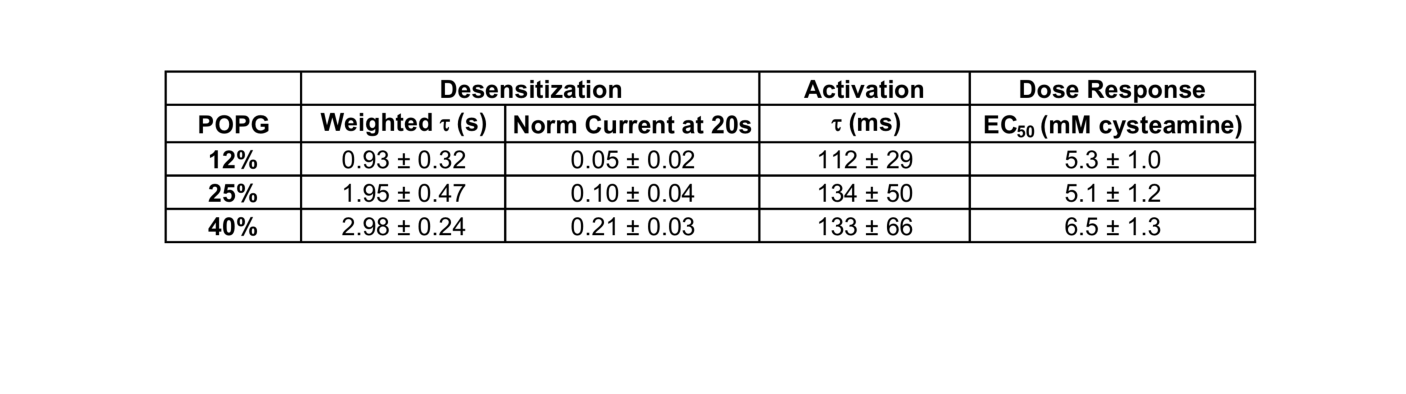
\includegraphics[width=\linewidth]{./pandoc_test/media/image3.pdf}
\caption[ELIC WT channel properties in giant liposomes composed of varying mole\% POPG (n=3-5, $\pm$SD).] {ELIC WT channel properties in giant liposomes composed of varying mole\% POPG (n=3-5, $\pm$SD). The rate and extent of desensitization are reported as weighted time constants ($\tau$), and the current after 20 s of 30 mM cysteamine application normalized to peak response. Also shown are activation time constants ($\tau$) in response to 30 mM cysteamine and EC50s for cysteamine activation.} \label{fig:three}
\end{figure*}

\begin{table}
    \caption{ELIC WT activation and desensitization rate constants derived from a double exponential fit to the time course of flux in Fig. \ref{fig:four}F (n=3, $\pm$SD). }
    \begin{tabular}{|c|c|c|}
	\hline
    {} & Activation Rate Constant & Desensitization RateConstant\\ \hline
    POPC & 24 $\pm$ 8 s\textsuperscript{-1} & 2.4 $\pm$ 0.08
    s\textsuperscript{-1}\\ \hline
    POPC:POPE:POPG (2:1:1) & 75 $\pm$ 22 s\textsuperscript{-1} & 0.11 $\pm$
    0.04 s\textsuperscript{-1}\\ \hline
    
    \end{tabular}
\end{table}


\begin{figure*}
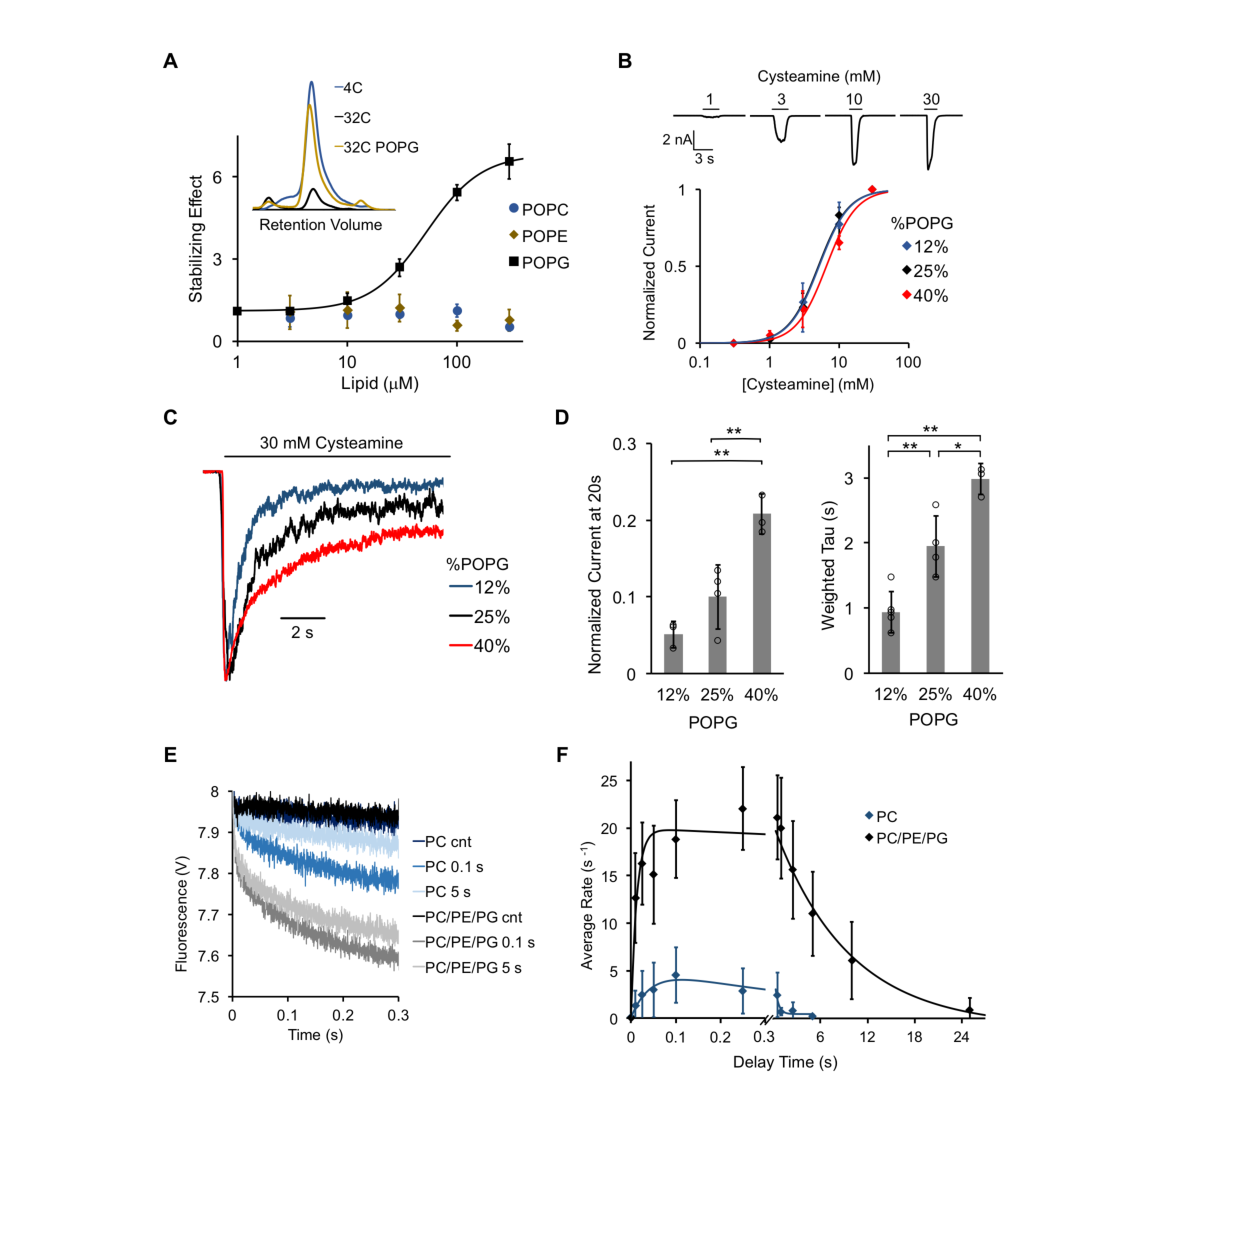
\includegraphics[width=\linewidth]{./pandoc_test/media/image4.pdf} 
\caption[POPG selectively thermally stabilizes ELIC and decreases ELIC desensitization.]{POPG selectively thermally stabilizes ELIC and decreases ELIC desensitization. Continued on the next page.}
\label{fig:four}
\end{figure*}

\begin{figure*}   
\caption[POPG selectively thermally stabilizes ELIC and decreases ELIC desensitization.] {POPG selectively thermally stabilizes ELIC and decreases ELIC desensitization. (A) Plot of stabilizing effect (defined as the ELIC pentamer peak height with phospholipid relative to control after heating) versus phospholipid concentration (n=3, $\pm$SD; EC50 = 52 $\mu$M, Hill n = 1.7). Inset shows size exclusion chromatography (SEC) profile in absorbance units of the ELIC pentamer treated at 4$^o$C, 32$^o$C, and 32$^o$C with 100 $\mu$M POPG. (B) Top: Representative ELIC current responses to 30 mM cysteamine in 25 mole\% POPG liposomes. Bottom: Normalized plots of peak current responses of ELIC to cysteamine in giant liposomes with varying mole\% POPG (n=3-5, $\pm$SD). Data are fit to Hill equation with n=2. (C) Representative ELIC currents in response to 30 mM cysteamine in liposomes with varying mole\% POPG. (D) Left: ELIC currents 20 s after application of 30 mM cysteamine normalized to peak response at varying mole\% POPG (n=4-5, $\pm$SD, **p$<$0.01). Right: Weighted tau (time constants) of ELIC desensitization at varying mole\% POPG (n=3-5, $\pm$ SD, **p$<$0.01, *p$<$0.05). (E) Representative fluorescence-quench time courses from sequential mixing stopped-flow experiments of ELIC in POPC liposomes or 2:1:1 POPC:POPE:POPG liposomes. Proteoliposomes were mixed with no cysteamine (cnt) or 5 mM cysteamine with a 0.1 or 5 s delay prior to mixing with Tl+. Note that the control traces are superimposed. (F) Rate constants extracted from quench kinetics as shown in (E) as a function of the incubation time with cysteamine. Data are fit with a double exponential yielding activation and desensitization time constants (n=3, $\pm$SD).} \label{fig:im4}
\end{figure*}


\subsection{Five interfacial arginines contribute to POPG binding}

\begin{figure*}
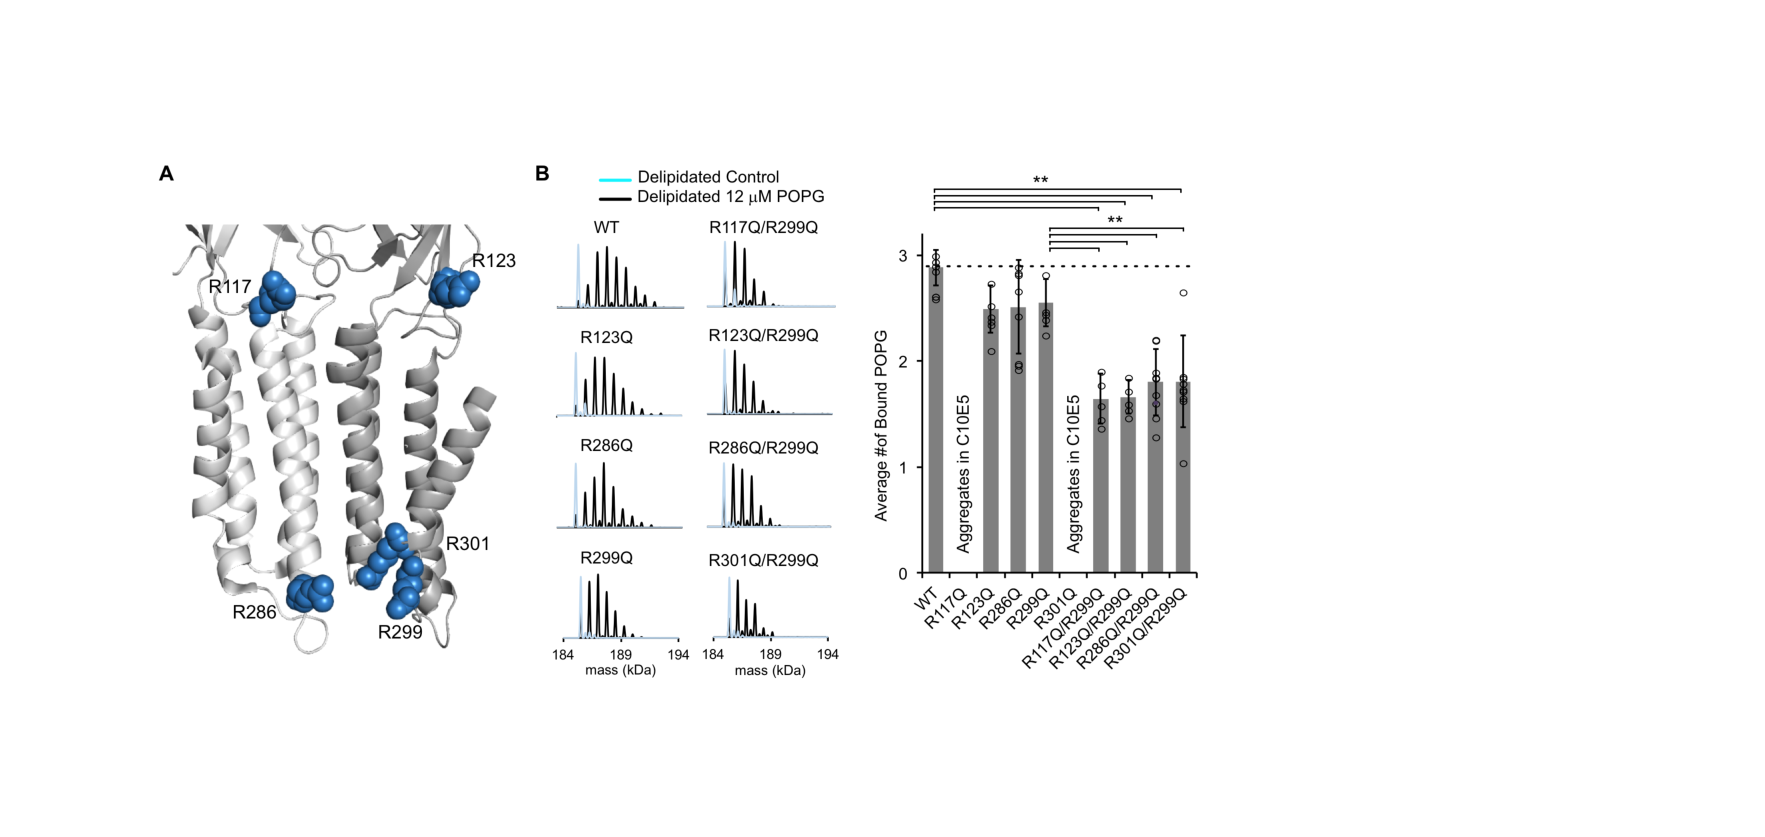
\includegraphics[width=1\linewidth]{./pandoc_test/media/image5.pdf}
\caption[Mutations of five interfacial arginines reduce POPG binding.] {Mutations of five interfacial arginines reduce POPG binding.(A) Structure of ELIC showing two adjacent subunits and five arginine side chains that were mutated to glutamine. (B) Left: Representative deconvoluted spectra of ELIC WT and indicated mutants. Blue indicates spectra of delipidated ELIC in C10E5. Black indicates spectra of delipidated ELIC in C10E5 with 12 $\mu$M POPG. Right: Plot of average number of bound POPG for ELIC WT and mutants, delipidated in C10E5, with 12 $\mu$M POPG (n=5-8, $\pm$SD, **p$<$0.01).} \label{fig:six}
\end{figure*}

In other ion channels, guanidine groups from interfacial arginine side
chains are thought to mediate binding of anionic phospholipids by charge
interactions with the phospholipid headgroup (9, 38). To test the
hypothesis that this mechanism is present in a pLGIC, we mutated all
five arginines in the inner and outer interfacial regions of the ELIC
TMD to glutamine (Fig. \ref{fig:six}A). Phospholipid binding was then assessed by
delipidating each mutant in C10E5, and measuring binding of POPG by
native MS. While R123Q, R286Q, and R299Q could be stably delipidated,
R117Q and R301Q aggregated (Fig. \ref{fig:six}B). However, we found that double
mutants with R299Q (i.e. R117Q/R299Q and R301Q/R299Q) could be stably delipidated. Thus, double
mutants of all arginine mutants in combination with R299Q were expressed
and delipidated (Fig. \ref{fig:six}B). In the presence of 12 $\mu$M POPG, the single
mutants showed moderate decreases (13-18\%) in the average number of
bound POPG compared to WT (Fig. \ref{fig:six}B). This decrease was not statistically
significant. However, all double mutants significantly decreased the
average number of bound POPG relative to WT by 38-41\% and relative to
R299Q by 27-32\% (Fig. \ref{fig:six}B). These results indicate that each interfacial
arginine contributes approximately equally to POPG binding in ELIC. It
is likely that significant decreases in binding could only be
appreciated in the double mutants because of the variability in the
data.

\begin{figure*}
\center
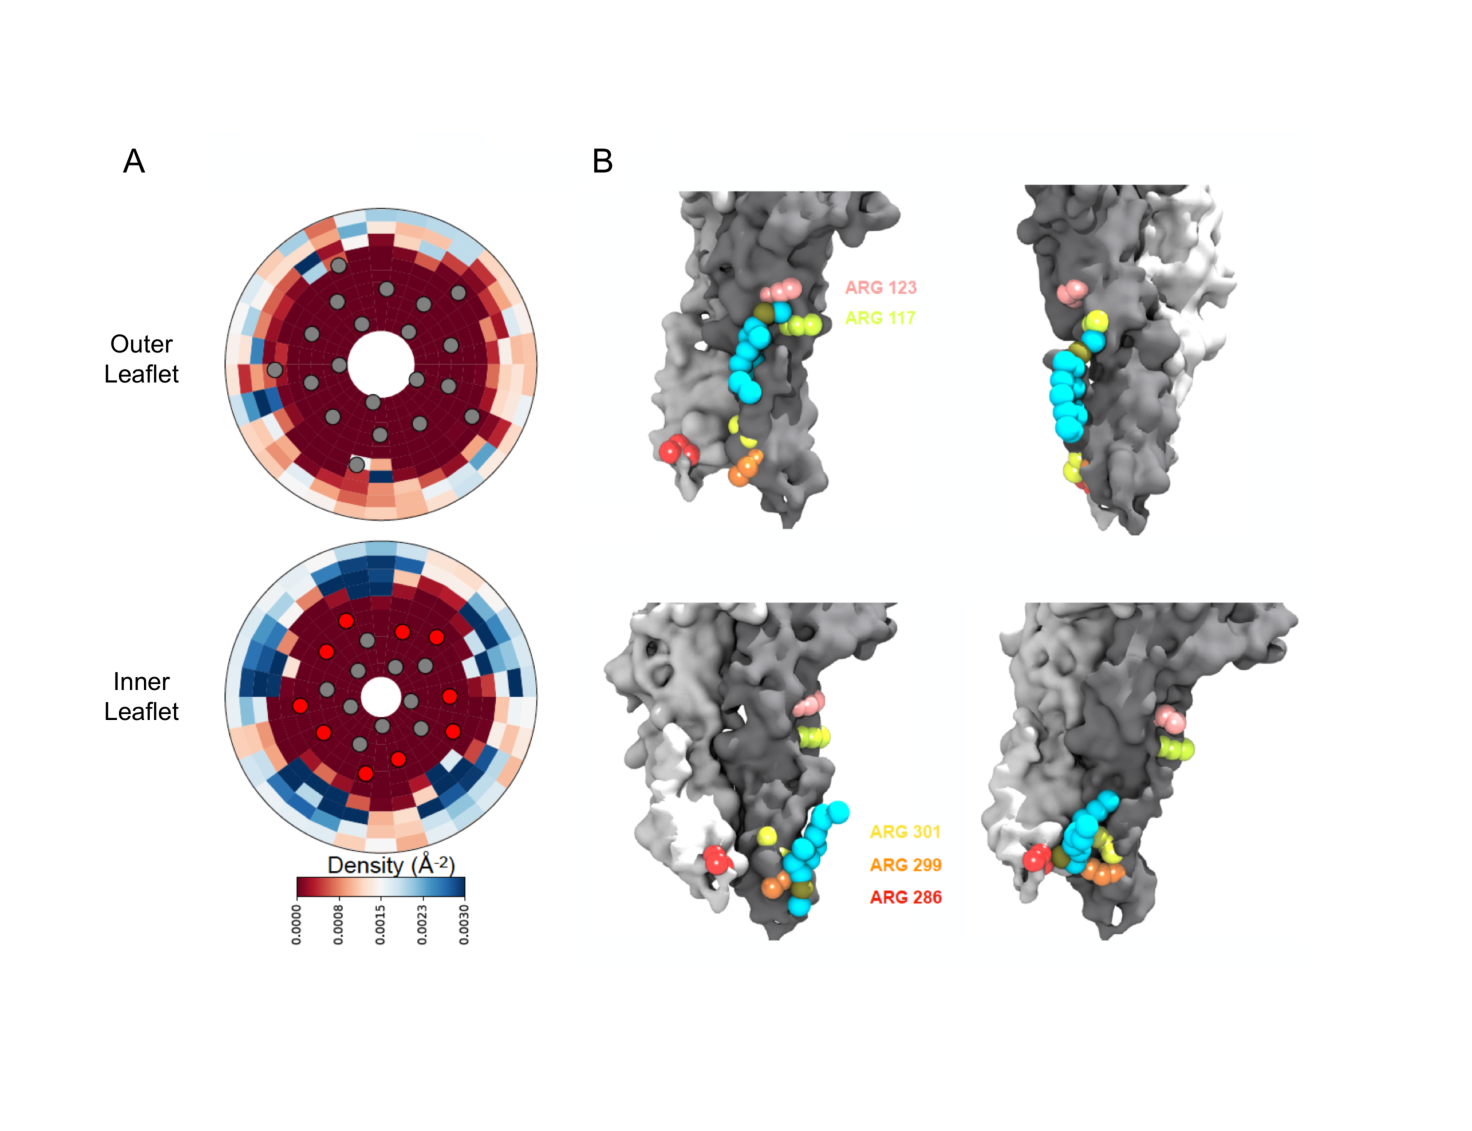
\includegraphics[width=\linewidth]{./pandoc_test/media/image6.pdf}
	\begin{flushleft}

\caption[Density calculations of lipids in binary membranes and visualization of direct POPG-ELIC interactions at 10\% POPG.] {Density calculations of lipids in binary membranes and visualization of direct POPG-ELIC interactions at 10\% POPG. (A) Distribution of POPG density in a POPG-POPC membrane, within 40 $\AA$ from the ELIC pore over the last half of a 15 $\mu$s simulation, for both the outer leaflet (top) and the inner leaflet (bottom). Density is colored according to the color bar, where red and blue represent low and high POPG density, respectively. Circles represent the ELIC transmembrane backbone center of mass, with the helices containing the interfacial arginines colored in red (B) Representative frames after ~9 $\mu$s of simulation, showing multiple POPG binding modes associated with high density areas in (A). Two adjacent subunits of ELIC are shown in grey and white, while arginine side chains of interest are colored in peach, lime-yellow, orange, yellow, and red. POPG phosphate is colored in tan with the rest of the lipid in cyan.} \label{fig:seven}
	\end{flushleft}

\end{figure*}



We further examined these sites of interaction using our coarse-grained
MD simulations. To identify whether boundary POPG were localized around
specific helices or residues, two-dimensional densities of the
negatively-charged headgroup bead were calculated. The distributions are
separated by leaflet where each leaflet contained 10\% POPG. As shown in
Fig. \ref{fig:seven}A, POPG was more likely to interact with ELIC in the inner
leaflet than the outer leaflet, consistent with three out of five
interfacial arginines residues being located on the intracellular
interface of the ELIC TMD. These three arginines are located on TM3
(R286) and TM4 (R299 and R301). Contacts between POPG and all three of
these residues are also visible in individual frames of the simulation
(Fig. \ref{fig:seven}B). Moreover, POPG is more likely to be contacting the
interfacial residues in TM4 (such as R299 and R301) than accessible
interfacial residues in any other helices (Fig. \ref{fig:seven}A). The remaining two
arginine residues are located at the TMD-ECD interface (R117 and R123).
POPG density in the outer leaflet localized to these residues at
intrasubunit sites between TM4 and TM1 or TM4 and TM3 (Fig. \ref{fig:seven}A), and
contacts between these residues and POPG headgroups in the outer leaflet
were also observed in snapshots from the MD simulations (Fig. \ref{fig:seven}B). In
summary, the native MS data and coarse-grained MD simulations
demonstrate that five interfacial arginines contribute to specific POPG
binding sites in the inner and outer leaflets adjacent to TM4.

\subsection{Specific interfacial arginines mediate POPG effect}

Having established that ELIC selectively binds POPG over neutral
phospholipids, and that binding is mediated by five interfacial
arginines, we examined the role of these binding sites on ELIC
desensitization. We reconstituted each single mutant into giant
liposomes composed of a 2:1:1 ratio of POPC:POPE:POPG (25\% POPG) to
test channel function by excised patch-clamping. We hypothesized that
since increasing mole\% POPG decreases ELIC desensitization, certain
arginine mutants, which disrupt POPG binding, may increase ELIC
desensitization. Indeed, all five single arginine mutants showed
variable increases in the rate or extent of desensitization; however,
these differences were generally small and statistically insignificant
except for R301Q (Fig. \ref{fig:eight}, Fig. \ref{fig:nine}). We also tested the double mutants,
which showed significant decreases in POPG binding. Three double mutants
(R117Q/R299Q, R123Q/R299Q, R301Q/R299Q) showed a significant increase in
the extent of desensitization while two (R117Q/R299Q, R301Q/R299Q) also
showed a significant increase in the rate of desensitization (Fig. \ref{fig:eight},
Fig. \ref{fig:nine}). The effects observed in the double mutants approximate the sum
of effects observed in the single mutants. Only R286Q/R299Q did not
affect the extent or rate of desensitization (Fig. \ref{fig:eight}, Fig. \ref{fig:nine}). The
EC\textsubscript{50} of cysteamine response and activation kinetics were
also measured for all mutants; only R117Q and R117Q/R299Q showed
significantly lower EC\textsubscript{50} and activation tau values
compared to WT (Fig. \ref{fig:nine}, Fig. \ref{fig:Supplementary Fig. 7}). Overall, these data
indicate that four of five interfacial arginine residues that reduce
POPG binding (i.e. R117, R123, R299, R301) also increase the rate and/or
extent of ELIC desensitization.

\subsection{L240A reduces desensitization and enhances POPG binding}

If mutations that disrupt POPG binding increase receptor
desensitization, then a mutation that decreases desensitization may
enhance POPG binding. Mutation of a conserved pore-facing 9' TM2 leucine
residue is known to slow desensitization in ELIC (L240A) (36) and other
pLGICs. To confirm this finding in our system, we reconstituted ELIC
L240A into giant liposomes for patch-clamping and observed a significant
reduction in the extent and rate of desensitization (Fig. \ref{fig:ten}A). To
examine POPG binding, L240A was then de-lipidated in C10E5 for native
MS. Interestingly, L240A significantly increased POPG binding compared
to WT at 12 $\mu$M POPG (\textasciitilde{}1.7x increase in average number of
POPG bound) (Fig. \ref{fig:ten}B).


\begin{figure*}

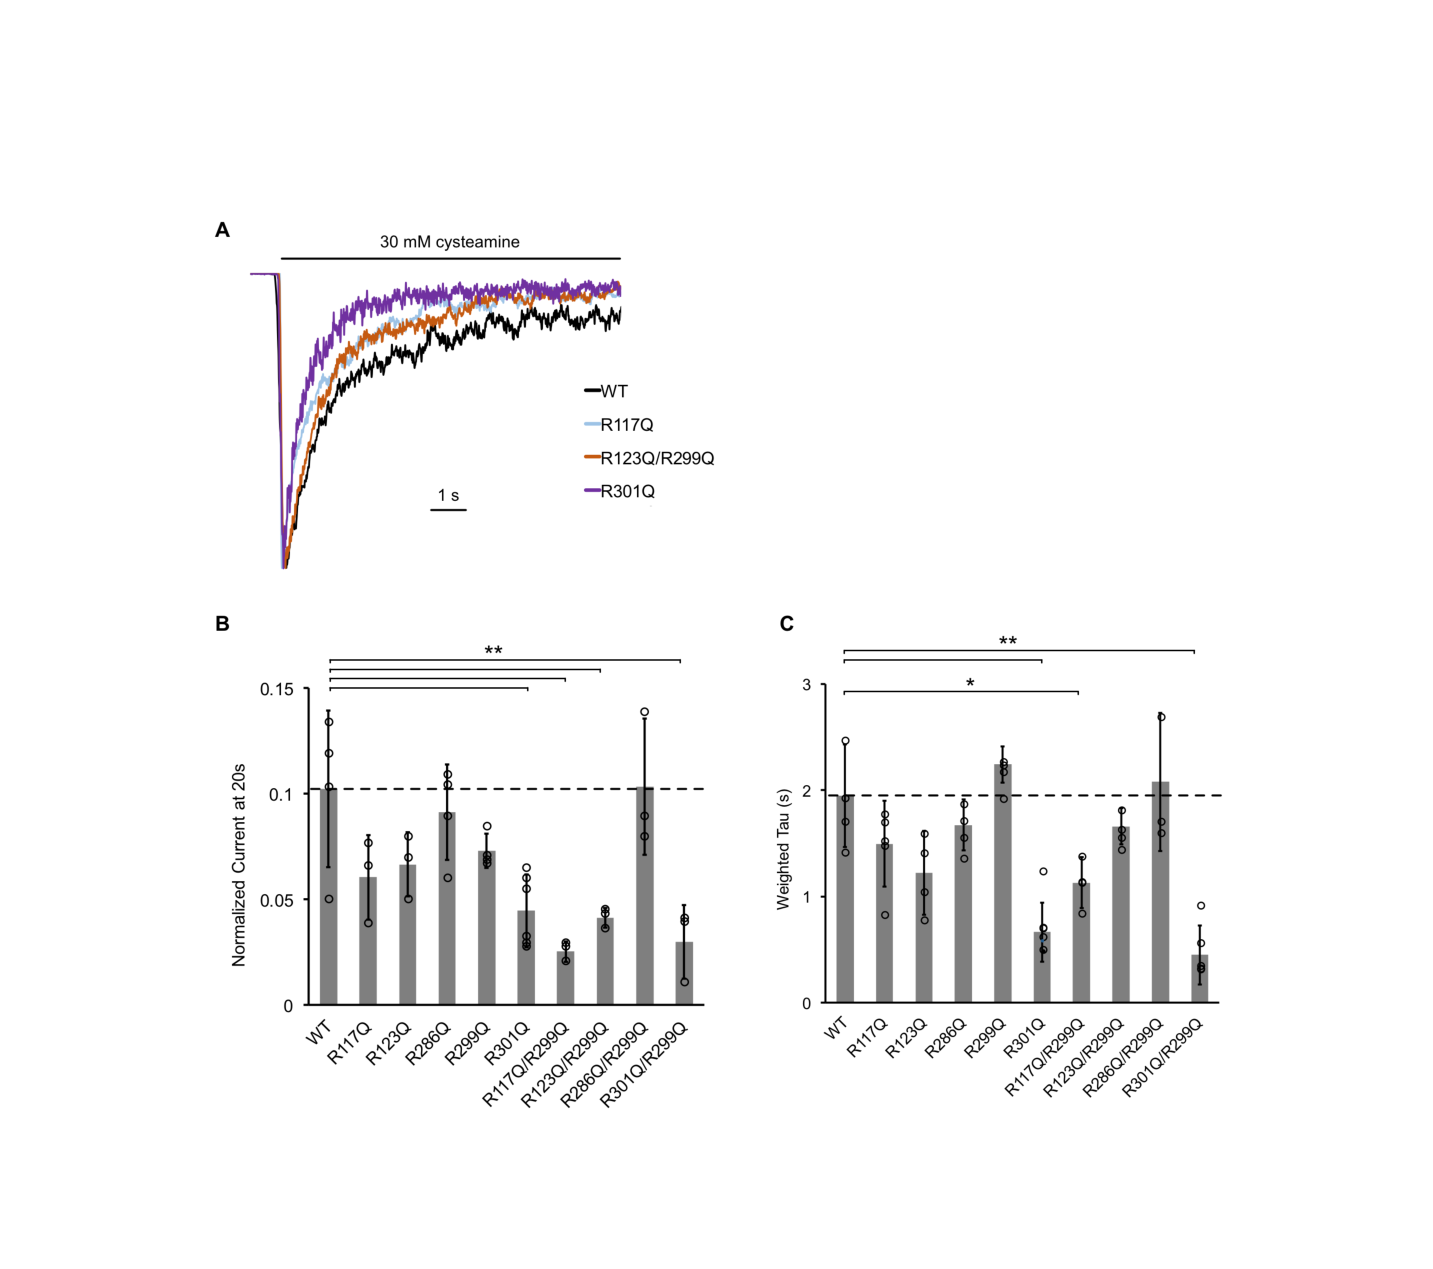
\includegraphics[width=\linewidth]{./pandoc_test/media/image7.pdf}

\caption[The effect of ELIC mutants on desensitization.] {The effect of ELIC mutants on desensitization. (A) Normalized ELIC WT and mutant current responses to 30 mM cysteamine in 25\% POPG liposomes. (B) Graph of ELIC WT and mutant currents 20 s after application of 30 mM cysteamine normalized to peak response in 25 mole\% POPG liposomes (n=3-7, $\pm$SD, **p$<$0.01, *p$<$0.05). (C) Same as (B) for weighted tau (time constants) of desensitization.} 
\label{fig:eight}

\end{figure*}

\section{Discussion}

Recent structural and computational evidence suggests that lipids bind
to pLGICs at specific sites within the TMD (24, 25, 39-41). However,
there is a scarcity of evidence showing that changes in direct lipid
binding are correlated with functional effects (25). We show that the
anionic phospholipid, POPG, selectively binds to ELIC using native MS,
thermally stabilizes the channel, and decreases receptor
desensitization. Overall, these data support the idea that lipid binding
directly affects receptor stability and function. Further, mutations of
arginine residues that reduce POPG binding also increase ELIC
desensitization to varying degrees. While it is possible that these
arginine mutations increase desensitization through a mechanism other
than their effect on POPG binding, the correlation between binding and
desensitization, and the finding that the L240A mutation, which reduces
desensitization, increases POPG binding affinity supports this
conclusion. Remarkably, the L240A mutation, which is located in the
channel pore and remote from the lipid interface (Fig. \ref{fig:eleven}), appears to
allosterically alter the affinity of ELIC for POPG. It is expected that
a mutation that stabilizes a higher affinity state of the receptor (e.g.
active over desensitized) would also enhance binding. Lipids may
modulate ion channel activity through indirect effects on the physical
properties of the membrane or through direct binding interactions (42,
43). The lipid binding data presented in this study using native MS
provides evidence that direct binding of anionic phospholipids
allosterically stabilizes the open state of a pLGIC relative to the
desensitized state.

\begin{figure*}

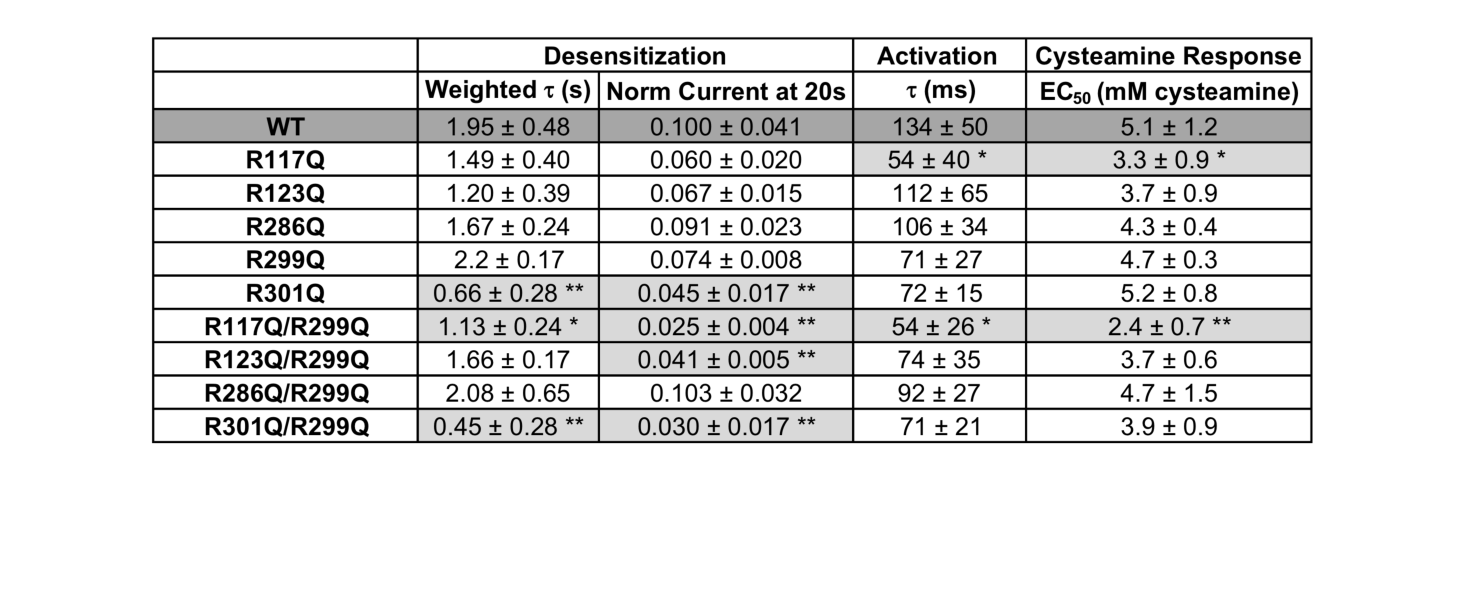
\includegraphics[width=\linewidth]{./pandoc_test/media/image8.pdf}

\caption[ELIC WT and mutant channel properties in giant liposomes composed of 25 mole\% POPG (n=3-7, $\pm$SD).] {ELIC WT and mutant channel properties in giant liposomes composed of 25 mole\% POPG (n=3-7, $\pm$SD). Shown are weighted time constants ($\tau$) for desensitization and currents 20 s after application of 30 mM cysteamine normalized to peak response. Also shown are activation time constants and EC50 of cysteamine response. Light gray indicates mutant values which are significantly different from WT (dark gray) (** p$<$0.01, * p$<$0.05).} 
\label{fig:nine}

\end{figure*}

Membrane proteins including pLGICs are thought to determine their lipid
microenvironment by specific binding interactions (28, 44). Our native
MS measurements provide unique insights into phospholipid interaction
with a pLGIC. First, we find that more POPG binds to ELIC compared to
POPE or POPC at equivalent concentrations, suggesting that POPG binds to
ELIC with higher affinity. This is supported by enrichment of POPG
compared to POPE in phospholipids that are co-purified with ELIC, and
coarse-grained simulations which show enrichment of POPG among the
boundary phospholipids of ELIC. Second, native MS also allows
determination of the stoichiometry and sites of lipid binding (32, 45).
By relating binding stoichiometry and thermal stability, the data
estimate that 32 POPG lipids, which is the average predicted number of
annular lipids in ELIC from MD simulations, results in greater than 80\%
of the stabilizing effect against thermal denaturation (Fig. \ref{fig:Supplementary
Fig. 5}), suggesting that maximal thermal stability is achieved when the
entire ELIC transmembrane domain (TMD) is surrounded by POPG. Although
five interfacial arginine residues were identified to contribute to POPG
binding in ELIC (25 arginines total), it is conceivable that each
arginine side chain may interact with more than one phospholipid
headgroup or that other sites exist.

To quantify the effect of the ELIC double mutants on specific POPG
binding sites, we also fit the native MS binding data for the double
mutants to a binomial binding model using the dissociation constant for
POPG binding to WT and varying the number of available sites. POPG
binding to the double mutants was best fit with a reduction in the
number of available sites from 32 in WT to 18-21 in the mutants
(Fig. \ref{fig:Supplementary Fig. 4}). Given the \textasciitilde{}35-45\% decrease in
bound phospholipid with each double mutant (mutation of two out of five
arginines), we conclude that phospholipid binding at these residues
constitute the highest affinity sites. This is indeed consistent with
the POPG densities from the coarse-grained simulations, which show
discrete enrichment of POPG lipids adjacent these residues. Disruption
of binding sites by mutation of these arginines may not prevent the
occupancy of lipids at these sites per se, but may alter the lipid
binding modes or occupancy times at these sites.

\begin{figure*}
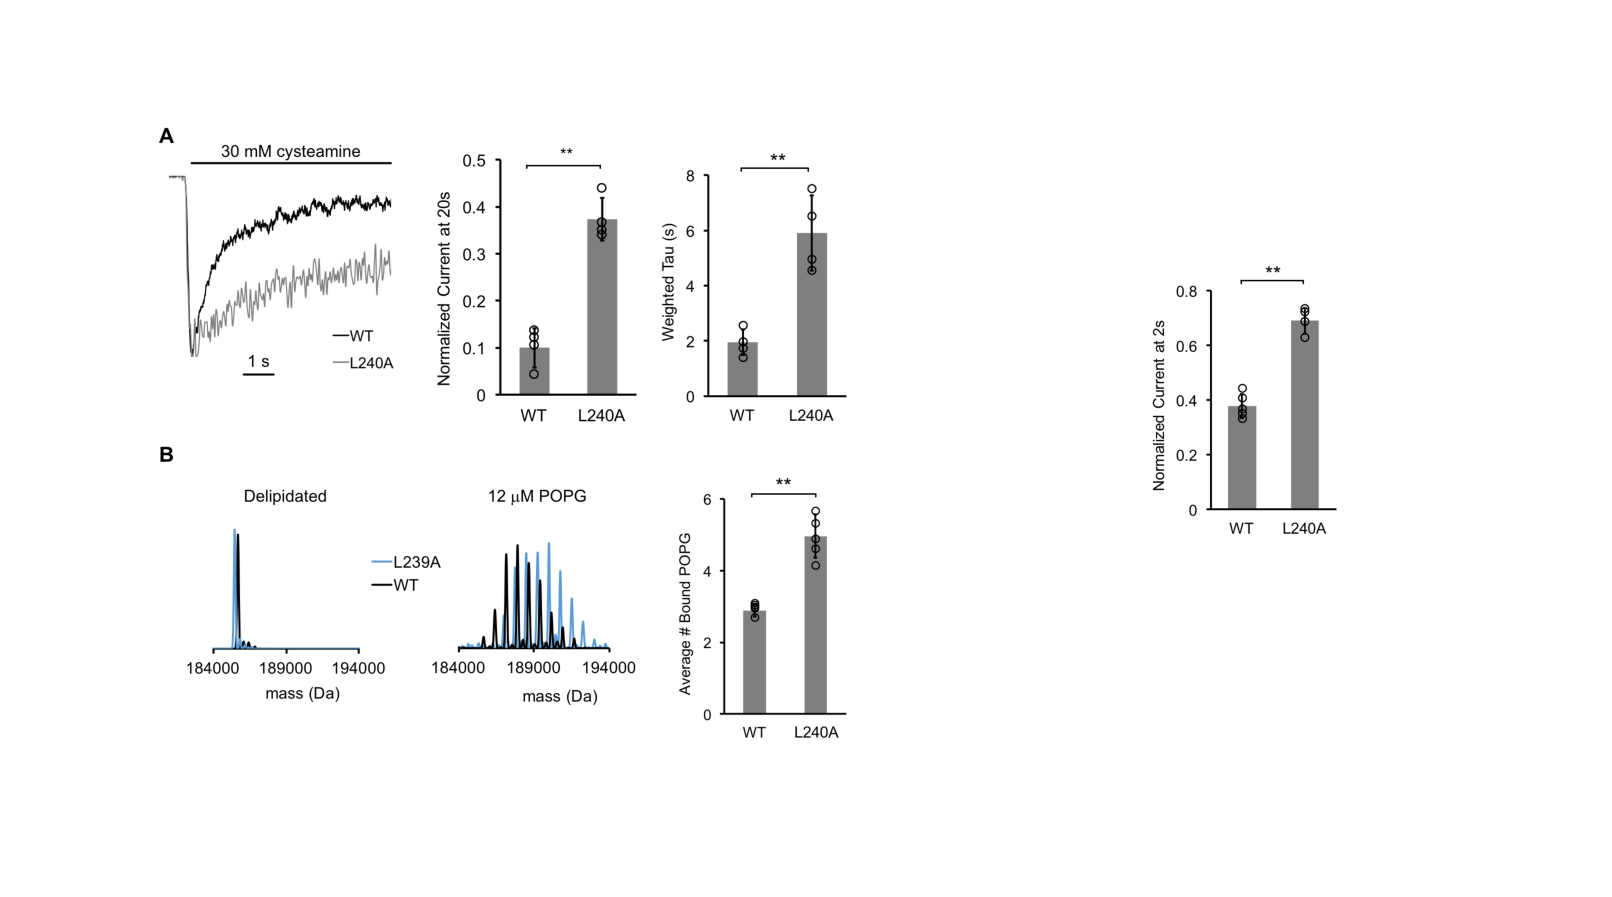
\includegraphics[width=\linewidth]{./pandoc_test/media/image9.pdf}
\caption[The L240A mutant decreases desensitization and increases POPG binding.] {The L240A mutant decreases desensitization and increases POPG binding. (A) Left: Normalized ELIC WT and L240A current responses to 30 mM cysteamine in 25\% POPG liposomes. Middle: ELIC WT and L240A currents 20 s after application of 30 mM cysteamine normalized to peak response at 25 mole\% POPG (n=4-5, $\pm$SD, **p$<$0.01). Right: Weighted tau (time constants) of ELIC WT and L240A desensitization time courses at 25 mole\% POPG (n=4-5, $\pm$SD, **p$<$0.01). (B) Left: Representative deconvoluted spectra of ELIC WT (black) and L240A (blue) showing ELIC delipidated in C10E5 without and with 12 $\mu$M POPG. Right: Graph of average number of bound POPG for ELIC WT and L240A, delipidated in C10E5, with 12 $\mu$M POPG (n=4-5, $\pm$SD, **p$<$0.01).}  \label{fig:ten}
\end{figure*}

Previous studies examining the effects of lipids on pLGIC function found
that nAchR and ELIC are inactive in POPC-only membranes (6, 15, 30), and
it was proposed that this is due to uncoupling of agonist binding to
channel activation (46). To examine ELIC channel activity in liposomes
lacking anionic phospholipid, we utilized a stopped-flow flux assay, and
demonstrated cysteamine-elicited flux by ELIC in POPC-only liposomes.
The high sensitivity of this assay may be the reason ELIC activity could
be detected, contrary to a prior study in which ELIC in POPC liposomes
were injected into \textit{Xenopus} oocytes (30). However, the ELIC
activity was significantly decreased compared to POPC:POPE:POPG (2:1:1)
liposomes. The low protein concentration used in this assay does not
allow us to assess the reconstitution efficiencies. Thus, the overall
lower flux rates and smaller amplitudes in POPC could stem from lower
protein reconstitution. However, the faster desensitization kinetics in
POPC liposomes can be resolved reliably, and are consistent with the
patch-clamp measurements. The results substantiate the role of POPG in
stabilizing the open state relative to the desensitized state, and
demonstrate the utility of measuring pLGIC activity in liposomes of
defined lipid composition using complementary
patch-clamp
and stopped-flow flux techniques.

\begin{figure*}
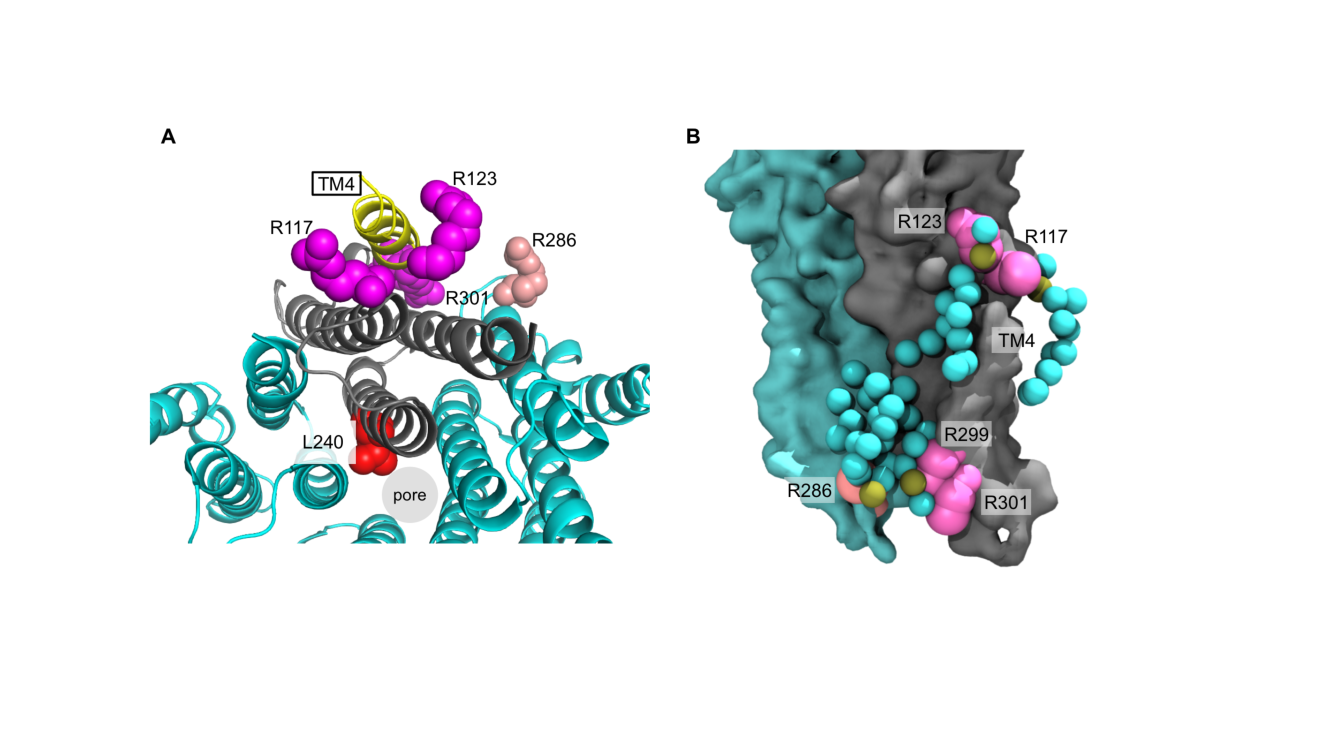
\includegraphics[width=\linewidth]{./pandoc_test/media/image10.pdf}
\caption[Arginines involved in POPG binding and ELIC desensitization.] {Arginines involved in POPG binding and ELIC desensitization. (A) Top view of ELIC highlighting TM4 (yellow) and showing the side chains of R117, R123 and R301 (magenta) adjacent to TM4, which increase ELIC desensitization, and R286 at the subunit interface (salmon), which has no effect on desensitization. L240 (red) faces the pore. (B) Image from coarse-grained simulations with 50\% POPG showing two adjacent ELIC subunits and the mutated arginine side chains (R117, R123, R299 and R301 in magenta; R286 in salmon). Also, shown are all POPG lipids making contacts with the TMD in this snapshot.} \label{fig:eleven}
\end{figure*}

While pLGICs are known to be sensitive to their lipid environment, the
binding sites that mediate lipid modulation are not well defined. It has
been proposed that TM4 is a lipid sensing structure in pLGICs due to its
proximity to the lipid membrane and sensitivity to mutagenesis (41,
47-49). Furthermore, crystal structures of GLIC show bound lipids within
intrasubunit grooves between TM4-TM1 and TM4-TM3 (23), which have been
proposed to be important determinants of channel opening (24, 25).
Photolabeling studies have also identified intrasubunit neurosteroid
binding sites adjacent to TM4 that mediate neurosteroid modulatory
effects (50, 51). We show that POPG binding at multiple interfacial
arginine residues, including R117, R124, R299 and R301 which are
localized to the extracellular and intracellular sides of TM4 (Fig. \ref{fig:eleven}),
are likely important in mediating the effect of POPG on ELIC
desensitization. Examination of boundary POPG from coarse-grained
simulations with high POPG mole\% (50\%) at 15 $\mu$s shows POPG headgroups
making contacts with all of these arginine side chains, and illustrates
potential binding modes for the acyl chains (Fig. \ref{fig:eleven}B). For example,
boundary POPG with headgroups that interact with R301 or R299 have acyl
chains that make contacts with intrasubunit sites along the
intracellular side of TM4 (Fig. \ref{fig:eleven}B and 5B). R301, which has the largest
effect on desensitization when mutated, is conserved among many
mammalian pLGICs including GABA\textsubscript{A}R and nAchR isoforms,
and R299 is adjacent to R301 at the bottom of TM4. Mutations in this
region of TM4 have profound effects on pLGIC desensitization (48, 49,
52, 53). R117 and R123 are located at the extracellular end of TM4, and
boundary POPG with headgroups that interact with these residues have
acyl chains that make contacts with intrasubunit sites on both sides of
TM4 (Fig. \ref{fig:eleven}B and 5B). Sites equivalent to R117 and R123 in GLIC were
previously found to be occupied by a phospholipid and docosahexaenoic
acid (DHA), respectively (24, 25). The polyunsaturated fatty acid, DHA,
was found to increase desensitization in GLIC (25). Therefore, it is
possible that the exact lipid structure occupying these sites results in
different effects. Our results raise the hypothesis that lipids with
polyunsaturated acyl chains or certain sterols (54) exert the opposite
effect of activating phospholipids by acting as competitive antagonists.

In summary, the anionic phospholipid, POPG, decreases desensitization in
the pLGIC, ELIC. POPG specifically binds to and stabilizes ELIC by
interacting with interfacial arginine residues. Our results strongly
suggest that binding of POPG at specific sites modulates receptor
desensitization.

\section{Methods}

\subsection{Mutagenesis, expression and purification of ELIC}

pET26-MBP-ELIC was a gift from Raimund Dutzler (Addgene plasmid \#
39239) and was used for WT ELIC expression and generation of mutants.
Site-directed mutagenesis was performed by the standard Quikchange
approach, and confirmed by Sanger sequencing (Genewiz, Plainfield, NJ).
WT and mutant ELIC was expressed as previously described (25, 55) in
OverExpressTM C43 (D3) \emph{E. coli} (Lucigen, Middleton, WI). Cultures
were grown in Terrific Broth (Sigma, St. Louis, MO) and induced with 0.1
mM IPTG for \textasciitilde{}16 hours at 18 \textsuperscript{o}C.
Pelleted cells were resuspended in Buffer A (20 mM Tris pH 7.5, 100 mM
NaCl) with cOmplete EDTA-free protease inhibitor (Roche, Indianapolis,
IN), and lysed using an Avestin C5 emulsifier at \textasciitilde{}15,000
psi. Membranes were collected by ultracentrifugation, resuspended in
Buffer A, solubilized in 1 \% DDM (Anatrace, Maumee, OH), and incubated
with amylose resin (New England Biolabs, Ipswich, MA) for 2 hours. The
resin was washed with 20 bed volumes of Buffer A, 0.02\% DDM, 0.5 mM
tris(2-carboxyethyl)phosphine (TCEP) and 1 mM EDTA, and eluted with
Buffer A, 0.02\% DDM, 0.05 mM TCEP, and 40 mM maltose. Eluted protein
was digested overnight with HRV-3C protease (Thermo Fisher, Waltham, MA)
(10 units per mg ELIC) at 4 \textsuperscript{o}C, and injected on a
Sephadex 200 10/300 (GE Healthcare Life Sciences, Pittsburgh, PA) size
exclusion column in Buffer A, 0.02\% DDM.

\subsection{Native MS measurements}

Native MS analysis was similar to previous descriptions for other
membrane proteins (27). For analysis of ELIC in DDM, 30 $\mu$l of purified
protein in 0.02\% DDM at \textasciitilde{}1 mg/ml was buffer exchanged
into 200 mM ammonium acetate pH 7.5 and 0.02\% DDM using Biospin 6 gel
filtration spin columns (Bio-Rad, Hercules, CA). 2 $\mu$l of buffer
exchanged ELIC was loaded into a borosilicate capillary emitter (Thermo
Scientific, Waltham, MA), and analyzed by static nanospray on a Thermo
QExactive EMR mass spectrometer. The following parameters were used to
resolve the ELIC pentamer and minimize dissociation into tetramer and
monomer: capillary voltage of 1.2 kV, capillary temperature of 200
\textsuperscript{o}C, ion transfer optics set with the injection
flatapole, inter-flatapole lens, bent flatapole, transfer multiple as 8,
7, 6, 4 V, respectively, resolution 8,750, AGC target 3 x
10\textsuperscript{6}, trap pressure set to maximum, CID 200 V, and CE
100 V. For analysis of ELIC in C10E5, ELIC delipidated by injecting 300
$\mu$g onto a Sephadex 200 10/300 column (GE Healthcare) at 0.5 ml/min
pre-equilibrated with Buffer A, 10\% glycerol, and 0.06\% C10E5
(Anatrace). 30 $\mu$l aliquots were then buffer exchanged to 100 mM ammonium
acetate pH 7.5, 0.06\% C10E5 using Biospin 6 columns, and diluted to 0.2
mg/ml. MS measurements on the QExactive EMR were performed with the
parameters listed above except: capillary temperature 100
\textsuperscript{o}C, CID 75 V and CE 200 V. For lipid binding
measurements, stocks of POPG lipid were prepared at 2x the concentration
of POPG being tested in 100 mM ammonium acetate pH 7.5 and 0.06\% C10E5.
Lipid stocks were then mixed with 0.4 mg/ml ELIC in a 1:1 volume ratio
for a final concentration of 1 $\mu$M ELIC, and samples were analyzed after
\textgreater{}5 min incubation.

MS spectra were deconvoluted using UniDec (56); deconvolution of spectra
with bound lipid was restricted to the +26 to +22 charge states
(Fig. \ref{fig:Supplementary Fig. 3}). Peak heights of apo and lipid-bound species were
extracted from UniDec, and analyzed by two approaches. The average
number of bound lipids was determined by the following relationship:
\begin{equation}
\mathrm{Average\ number\ bound\ lipid = \ }\frac{\sum_{\mathrm{n = 0}}^{\mathrm{k}}{\mathrm{n \cdot}\mathrm{I}_{\mathrm{n}}}}{\sum_{\mathrm{n = 0}}^{\mathrm{k}}\mathrm{I}_{\mathrm{n}}}
\end{equation}
where n is the number of bound lipids and I\textsubscript{n} is the
deconvoluted peak height of ELIC with n bound lipids. Peak heights of
apo and lipid-bound species were also plotted as mole fraction versus
the number of bound lipids (Fig. \ref{fig:Supplementary Fig. 4}). These data were fit
with a binomial binding model, which assumes that there are N sites each
with equal affinity, K. The probability, p, that a site is occupied at
the concentration of a given lipid, A, is defined as:

\begin{equation}
p = \frac{\lbrack A\rbrack}{\left\lbrack A \right\rbrack + K}
\end{equation}

Then, the probability (B) that q sites are occupied out of N total sites
is given by the binomial probability function:

\begin{equation}
B\left( q \right) = \ \frac{N!}{q!\left( N - q \right)!}p^{N - q}{(1 - p)}^{q}
\end{equation}

B(q) was used to determine the mole fraction of each lipid-bound species
at a given {[}A{]}, which was used to fit the native MS data in Excel
across all {[}A{]} by setting K constant and varying N or vice versa.

\subsection{Thermal stability assay}

Purified WT ELIC in C10E5 (Buffer A, 0.06\% C10E5) was diluted to 1 $\mu$M
in the absence or presence of various concentrations of phospholipid.
Samples were analyzed without and with heating in the absence or
presence of phospholipid. Analysis of protein thermal stability was
performed by injecting 90 $\mu$l of sample on a size exclusion column
(Sephadex 200 10/300), and measuring the amplitude of the pentamer peak
as previously described (57, 58). Heating was performed for 15 min at 32
\textsuperscript{o}C, which resulted in a \textasciitilde{}85\% decrease
in the pentamer amplitude compared to 4\textsuperscript{o}C. The
stabilizing effect of a phospholipid was quantified as the pentamer
amplitude in the presence of phospholipid (heated) divided by control
(heated).

\subsection{Excised patch-clamp recordings from giant liposomes}

ELIC WT and mutants were reconstituted into giant liposomes as
previously described with some modifications (59). Three liposome
preparations were used in this study: 1) 25\% POPG (consists of 50\%
POPC/ 25\% POPE/ 25\% POPG), 2) 12\% POPG (consists of 60\% POPC/ 28\%
POPE/ 12\% POPG), and 3) 40\% POPG (consists of 35\% POPC/ 25\% POPE/
40\% POPG). These liposome compositions were chosen to vary POPG mole\%
while optimizing lipid mixtures to obtain ideal giant liposomes for
patch-clamping. This was achieved by varying POPG mole\% and POPC mole\%
inversely. Condition \#1 was used for WT and all mutants, and conditions
\#2 and \#3 were used in WT. Liposomes were prepared by drying 15-20 mg
of lipid mixtures in chloroform using N\textsubscript{2} in a round
bottom flask and then overnight in a vacuum dessicator. Dried lipids
were rehydrated at 5 mg/ml in 10 mM MOPS pH 7, and 150 mM NaCl (MOPS
buffer), subjected to ten freeze-thaw cycles ten, and then small
unilamellar liposomes were formed by extrusion using a 400 nm filter
(Avanti Lipids, Alabaster, AL) and bath sonication (30 sec x 5). 5 mg of
liposomes in 1 ml were destabilized by adding DDM to 0.2\% and rotating
for 1 hour at room temperature followed by 0.3-0.5 mg of ELIC WT or
mutants at \textasciitilde{}4-5 mg/ml and incubation for 30 min. To
remove DDM, SM-2 Bio-beads (Bio-Rad) were added in five batches (30, 30,
50, 100, and 100 mg). The first three batches were added each hour along
with 1 ml of MOPS buffer to make a final volume of 4 ml while rotating
at room temperature. After adding the first 100 mg batch, the
proteoliposomes were rotated overnight at 4 \textsuperscript{o}C,
followed by the last 100 mg the next day for 3 hours at room
temperature. Proteoliposomes were harvested by ultracentrifugation at
150,000 x \emph{g} for 1 hour at 4 \textsuperscript{o}C, and the pellet
resuspended with 80 $\mu$l of MOPS buffer for a lipid concentration of
\textasciitilde{}50 mg/ml. Giant liposomes were formed by drying 10 $\mu$l
of proteoliposomes on a glass coverslip in a desiccator for 3-5 hours at
4 \textsuperscript{o}C followed by rehydration with 60 $\mu$l of MOPS buffer
overnight at 4 \textsuperscript{o}C and at least 2 hours at room
temperature the next day. Giant liposomes were resuspended by pipetting
and then applied to a petri dish with MOPS buffer.

Patch-clamp recordings were performed using borosilicate glass pipettes
pulled to $\sim2-3$ M$\Omega$ using a P-2000 puller (Sutter
instruments, Novato, CA). Pipettes were filled with 10 mM MOPS pH 7, 150
mM NaCl, and 0.5 mM BaCl$_{2}$. Excised patches (the
orientation of ELIC in the liposomes is not known; therefore, these
patches are not defined as outside-out or inside-out) were held at -60
mV, and bath solutions consisted of 10 mM MOPS pH 7, 150 mM NaCl, 0.5 mM
BaCl$_{2}$, 1 mM DTT, and varying concentrations of
cysteamine. DTT was added to the bath solution to prevent cysteamine
oxidation. Rapid solution exchange was achieved with a three-barreled
flowpipe mounted and adjusted by to a SF-77B fast perfusion system
(Warner Instrument Corporation, Hamden, CT). Liquid junction current at
the open pipette tip demonstrated 10-90\% exchange times of
\textless{}10 ms. Data was collected at 20 kHz using an Axopatch 200B
amplifier (Molecular Devices, San Jose, CA) and a Digidata 1322A
(Molecular Devices) with Axopatch software, and a low pass Bessel filter
of 10 kHz was applied to the currents. Analysis of currents was
performed with Clampfit 10.4.2 (Molecular Devices). Activation currents
were fit to a single exponential equation, and desensitization currents
were fit to both single and double exponential equations. The majority
of desensitization currents were best fit with a double exponential, and
weighted time constants were derived using the following calculation:

\begin{equation}
Weighted \tau = \frac{\left( A1 \cdot \tau 1 \right) + (A2 \cdot \tau 2)}{A1 + A2}
\end{equation}

where A1 and A2 are the weighted coefficients of the first and second
exponential components. The reported weighted average time constants are
averages of weighted time constants from double exponential fits and
time constants from single exponential fits. Peak cysteamine dose
response curves were fit to a Hill equation, keeping n constant at 2,
which provided a reasonable fit for all data sets. All statistical
comparisons were made using a one-way ANOVA with post-hoc Tukey HSD
test.

\subsection{Stopped-flow fluorescence recordings}

The fluorescence-based sequential-mixing stopped-flow assay was carried
out with an SX20 stopped-flow spectrofluorimeter (Applied Photophysics,
Leatherhead, UK) at 25 \textsuperscript{o}C. To reconstitute ELIC into
large unilamellar vesicles (LUVs), 15 mg of lipids (POPC or
POPC:POPE:POPG 2:1:1) were dried in glass vials to a thin film under a
constant N\textsubscript{2} stream. Lipids were further dried under
vacuum overnight. The next day, lipids were rehydrated in reconstitution
buffer (1114 $\mu$l of 15 mM Hepes, 150 mM NaNO\textsubscript{3}, pH 7). 33
mg CHAPS were added stepwise while sonicating lipids in a bath sonicator
until the solution was clear. 1057 $\mu$l of a 75 mM ANTS stock solution (in
ddH\textsubscript{2}O, pH 7) was added together with purified ELIC (1
$\mu$g/mg lipid), mixed and incubated for 20 min. Detergent removal was
initiated by addition of 0.7 g SM-2 BioBeads (BioRad) in assay buffer
(10 mM Hepes, 140 mM NaNO\textsubscript{3}, pH 7). The reconstitution
mix was incubated for 2.5 h at 21 \textsuperscript{o}C under gentle
agitation. The liposome-containing supernatant was transferred to a new
glass tube and stored overnight at 13 \textsuperscript{o}C. The liposome
solution was sonicated in a bath sonicator for 30 s and extruded through
a 0.1 $\mu$m membrane (Whatman) using a mini-extruder (Avanti Polar lipids).
Extra-vesicular ANTS were removed with a 10 ml desalting column (PD-10,
GE Lifesciences). Right before the assay, liposomes were diluted 5-fold
in assay buffer to ensure a good signal to noise ratio.

For the assay, ELIC-containing liposomes were mixed 1:1 with pre-mix
buffer (assay buffer supplemented with 10 mM cysteamine to reach 5 mM
after mixing) and incubated for defined amounts of time (10 ms -- 25 s).
A second 1:1 mixing step was performed with quenching buffer (10 mM
Hepes, 90 mM NaNO\textsubscript{3}, 50 mM TlNO\textsubscript{3}, pH 7).
ANTS fluorescence was excited at 360 nm and the integral fluorescence
above 420 nm was recorded for 1 s. For each delay time, at least 8
repeats under identical conditions were performed.

To analyze the data, each repeat was visually inspected and outliers
were removed. Each remaining repeat was then fitted to a stretched
exponential (Equation 4.1) and the rate of Tl+ influx was determined at 2
ms (Equation 4.2).
\begin{equation}
F_{t} = F_{\infty}\  + \ \left( F_{0}\  - \ F_{\infty} \right)\  \cdot \ e^{\left\{ - \ \left( \frac{t}{\tau} \right)^{\beta} \right\}}
\end{equation}
\begin{equation}
k_{t} = \ \left( \frac{\beta}{\tau} \right)\  \cdot \ \left( \frac{2\ ms}{\tau} \right)^{\left( \beta\  - 1 \right)}\ 
\end{equation}
with F\textsubscript{t}, F\textsubscript{$\infty$}, F\textsubscript{0} being
the fluorescence at time t, the final fluorescence and the initial
fluorescence, respectively. t is the time (in s), $\tau$ the time constant
(in s) and \emph{$\beta$} the stretched exponential factor.
\emph{k}\textsubscript{t} is the calculated rate (in
s\textsuperscript{-1}) of Thallium influx at 2 ms.

The rate constants were averaged and the mean and standard deviations
(S.D.) were determined and plotted (Fig 2F). The experiments were
repeated for each lipid composition using three independent
reconstitutions. The rates and S.D. were averaged and plotted as
function of the delay time. The time course was fitted according to a
double-exponential function to obtain the rates of activation and
desensitization, respectively.

\subsection{Lipid extraction and MS analysis}

Lipids were extracted using a Bligh-Dyer extraction (60). Briefly, 100
$\mu$g of purified ELIC in DDM and 150 $\mu$g of \emph{E. coli} membranes
derived from cell cultures transformed and induced for ELIC expression,
respectively, were mixed with 1 ml chloroform, 2 ml methanol and 0.8 ml
water, and vortexed for 1 min, followed by an additional 1 ml chloroform
and 1 ml water, and vortex for 3 min. The samples were centrifuged for 3
min at 500 x \emph{g}, and the lower organic phase removed for analysis,
using a Thermo Scientific LTQ Orbitrap Velos mass spectrometer. Lipid
extracts were loop injected (1.5 $\mu$l/min) using a syringe pump that
delivered a continuous flow of methanol at 15 $\mu$l/min into the ESI
source. High resolution (R = 100,000 at m/z 400) MS and MS/MS analyses
were performed in negative ion mode. The skimmer of the ESI source was
set at ground potential, electrospray voltage 4 kV, capillary
temperature 300 \textsuperscript{o}C, AGC target 5 x
10\textsuperscript{4}, and maximum injection time 50 ms.
MS\textsuperscript{n} experiments for identification of lipid structures
were carried out with an optimized relative collision energy of 32\%,
activation q value of 0.25, activation time of 10 ms, and mass selection
window of 1 Da.

\subsection{Coarse-grained simulations of ELIC}

All simulations reported here used the MARTINI 2.2 (61) coarse-grained
topology and force field. The crystal structure of ELIC (PDB 3RQW) (62)
was coarse-grained using MARTINI martinize.py script. Secondary
structural restraints were constructed using martinize.py while imposed
through Gromacs (63). Conformational restraints were preserved through
harmonic bonds between backbone beads less than 0.5 nm apart with a
coefficient of 900 kJ mol\textsuperscript{-1}. Pairs were determined
using the ElNeDyn algorithm (64). Membranes were constructed using the
MARTINI script insane.py (61). The insane.py script randomly places
lipids throughout both inner and outer membranes and embeds selected
proteins into the membrane. Two series of simulations were developed,
the first using POPE and POPG, and the second POPC and POPG. Box sizes
were about 30 x 30 x 25 nm\textsuperscript{3} and each simulation box
contained about 3000 lipids.

Molecular dynamics simulations were carried out using GROMACS 5.1.4
(63). All systems were run using van der Waals (vdW) and electrostatics
in cutoff and reaction-field, respectively, with a dielectric constant
of \(\varepsilon = 15\). vdW and electrostatics used a cutoff length of
1.1 nm as defined in current MARTINI build specifications. Energy
minimizations were performed for about 30,000 steps. All systems were
run for short equilibration steps. Canonical ensembles (NVT) were run
for 100 ps using Berendsen thermostat set to 323 K with the temperature
coupling constant set to 1 ps. Isothermal-Isobaric ensemble (NPT)
equilibration was run for 5000 ps using Berendsen thermostat and
barostat. The thermostat was set to 323 K with the temperature coupling
constant set to 1 ps, and the barostat was set to a pressure coupling
constant of 3 ps with a compressibility of 3 x 10\textsuperscript{-5}
bar\textsuperscript{-1} holding at 1 bar. Molecular dynamics were
carried out using NPT ensemble and were simulated for 15 $\mu$s with a time
step of 0.015 ps using v-rescale thermostat set to 323 K and a
temperature coupling constant of 1 ps. Membranes consisting of POPE used
the Parrinello-Rahman barostat, and membranes consisting of POPC used
the Berendsen barostat, both under semi-isotropic coupling. The
reference pressure was set to 1 bar, the compressibility
3x10\textsuperscript{-4} bar\textsuperscript{-1}, and the pressure
coupling constant 1 ps.

Annular lipids were determined using the annular lipid metric B:
\begin{equation}
B_{i} = \left\langle \frac{b_{i}}{b_{\text{tot}}} \right\rangle\frac{1}{x_{i}} - 1
\end{equation}

where \(b_{i}\) is the instantaneous number of boundary lipids of
species \(i\), \(b_{\text{tot}}\) is the instantaneous total number of
boundary lipids, \(x_{i}\) is the overall (bulk) fraction of species
\(i\) and the brackets represent an average over time and replicas.
\(B_{i}\) \textless{} 0 and \(B_{i}\) \textgreater{} 0 indicate
enrichment and depletion of species \(i\), respectively, relative to the
abundance in the bulk membrane. A given lipid was counted as a boundary
lipid if it was within 6 Å of the ELIC transmembrane domain.

Two dimensional lipid density distributions around a central ELIC
pentamer were calculated for each leaflet using polar coordinates (28).
For every sampled frame, all lipids of species \(i\) were separated into
leaflets. For all \(i\) lipids in a given leaflet, the vector separating
the phosphate beads from ELIC center was calculated and projected onto
the membrane plane. The two-dimensional separation vector was then used
to assign the lipid to the appropriate polar bin of radial bin width
\(4\mathring{\mathrm{A}}\) and angular bin width
\(\frac{\pi}{15}\text{.\ }\)The area density in each bin was averaged
over time and replicas.

\textbf{\emph{\\
}}

\textbf{\emph{Acknowledgements}}

We are grateful to Alex Evers, Joe Henry Steinbach, Christopher Lingle
and Gustav Akk for helpful discussions and edits regarding this study
and the preparation of the manuscript. We also acknowledge Arthur
Laganowsky and Yang Liu for guidance with regard to sample preparation
of ELIC for native MS measurements. We are indebted to Michael Gross at
the Washington University NIH/NIGMS-supported biomedical mass
spectrometry resource for use of the Thermo QExactive EMR mass
spectrometer, and Christopher Lingle for use of a patch-clamp rig for
electrophysiology recordings.

\textbf{\emph{Competing Interests}}

The authors declare that no competing interests exist.

\section{Reference}

1. Corringer PJ, Poitevin F, Prevost MS, Sauguet L, Delarue M, Changeux
JP. Structure and pharmacology of pentameric receptor channels: from
bacteria to brain. Structure. 2012;20(6):941-56.

2. Allen JA, Halverson-Tamboli RA, Rasenick MM. Lipid raft microdomains
and neurotransmitter signalling. Nat Rev Neurosci. 2007;8(2):128-40.

3. Baenziger JE, Henault CM, Therien JP, Sun J. Nicotinic acetylcholine
receptor-lipid interactions: Mechanistic insight and biological
function. Biochim Biophys Acta. 2015;1848(9):1806-17.

4. Rosenhouse-Dantsker A, Mehta D, Levitan I. Regulation of ion channels
by membrane lipids. Compr Physiol. 2012;2(1):31-68.

5. Evers AS, Elliott WJ, Lefkowith JB, Needleman P. Manipulation of rat
brain fatty acid composition alters volatile anesthetic potency. J Clin
Invest. 1986;77(3):1028-33.

6. Criado M, Eibl H, Barrantes FJ. Functional properties of the
acetylcholine receptor incorporated in model lipid membranes.
Differential effects of chain length and head group of phospholipids on
receptor affinity states and receptor-mediated ion translocation. J Biol
Chem. 1984;259(14):9188-98.

7. Cheng WW, D'Avanzo N, Doyle DA, Nichols CG. Dual-mode phospholipid
regulation of human inward rectifying potassium channels. Biophys J.
2011;100(3):620-8.

8. Chemin J, Patel AJ, Duprat F, Lauritzen I, Lazdunski M, Honore E. A
phospholipid sensor controls mechanogating of the K+ channel TREK-1.
EMBO J. 2005;24(1):44-53.

9. Hite RK, Butterwick JA, MacKinnon R. Phosphatidic acid modulation of
Kv channel voltage sensor function. Elife. 2014;3.

10. Schmidt D, Jiang QX, MacKinnon R. Phospholipids and the origin of
cationic gating charges in voltage sensors. Nature.
2006;444(7120):775-9.

11. Zolles G, Klocker N, Wenzel D, Weisser-Thomas J, Fleischmann BK,
Roeper J, et al. Pacemaking by HCN channels requires interaction with
phosphoinositides. Neuron. 2006;52(6):1027-36.

12. daCosta CJ, Medaglia SA, Lavigne N, Wang S, Carswell CL, Baenziger
JE. Anionic lipids allosterically modulate multiple nicotinic
acetylcholine receptor conformational equilibria. J Biol Chem.
2009;284(49):33841-9.

13. Hamouda AK, Sanghvi M, Sauls D, Machu TK, Blanton MP. Assessing the
lipid requirements of the Torpedo californica nicotinic acetylcholine
receptor. Biochemistry. 2006;45(13):4327-37.

14. daCosta CJ, Wagg ID, McKay ME, Baenziger JE. Phosphatidic acid and
phosphatidylserine have distinct structural and functional interactions
with the nicotinic acetylcholine receptor. J Biol Chem.
2004;279(15):14967-74.

15. Ochoa EL, Dalziel AW, McNamee MG. Reconstitution of acetylcholine
receptor function in lipid vesicles of defined composition. Biochim
Biophys Acta. 1983;727(1):151-62.

16. Fong TM, McNamee MG. Correlation between acetylcholine receptor
function and structural properties of membranes. Biochemistry.
1986;25(4):830-40.

17. Baenziger JE, Morris ML, Darsaut TE, Ryan SE. Effect of membrane
lipid composition on the conformational equilibria of the nicotinic
acetylcholine receptor. J Biol Chem. 2000;275(2):777-84.

18. Velisetty P, Chakrapani S. Desensitization mechanism in prokaryotic
ligand-gated ion channel. J Biol Chem. 2012;287(22):18467-77.

19. Ellena JF, Blazing MA, McNamee MG. Lipid-protein interactions in
reconstituted membranes containing acetylcholine receptor. Biochemistry.
1983;22(24):5523-35.

20. Mantipragada SB, Horvath LI, Arias HR, Schwarzmann G, Sandhoff K,
Barrantes FJ, et al. Lipid-protein interactions and effect of local
anesthetics in acetylcholine receptor-rich membranes from Torpedo
marmorata electric organ. Biochemistry. 2003;42(30):9167-75.

21. Dreger M, Krauss M, Herrmann A, Hucho F. Interactions of the
nicotinic acetylcholine receptor transmembrane segments with the lipid
bilayer in native receptor-rich membranes. Biochemistry.
1997;36(4):839-47.

22. Antollini SS, Barrantes FJ. Disclosure of discrete sites for
phospholipid and sterols at the protein-lipid interface in native
acetylcholine receptor-rich membrane. Biochemistry.
1998;37(47):16653-62.

23. Bocquet N, Nury H, Baaden M, Le Poupon C, Changeux JP, Delarue M, et
al. X-ray structure of a pentameric ligand-gated ion channel in an
apparently open conformation. Nature. 2009;457(7225):111-4.

24. Prevost MS, Sauguet L, Nury H, Van Renterghem C, Huon C, Poitevin F,
et al. A locally closed conformation of a bacterial pentameric
proton-gated ion channel. Nat Struct Mol Biol. 2012;19(6):642-9.

25. Basak S, Schmandt N, Gicheru Y, Chakrapani S. Crystal structure and
dynamics of a lipid-induced potential desensitized-state of a pentameric
ligand-gated channel. Elife. 2017;6.

26. Laganowsky A, Reading E, Allison TM, Ulmschneider MB, Degiacomi MT,
Baldwin AJ, et al. Membrane proteins bind lipids selectively to modulate
their structure and function. Nature. 2014;510(7503):172-5.

27. Gault J, Donlan JA, Liko I, Hopper JT, Gupta K, Housden NG, et al.
High-resolution mass spectrometry of small molecules bound to membrane
proteins. Nat Methods. 2016;13(4):333-6.

28. Sharp L, Salari R, Brannigan G. Boundary lipids of the nicotinic
acetylcholine receptor: Spontaneous partitioning via coarse-grained
molecular dynamics simulation. Biochim Biophys Acta Biomembr.
2019;1861(4):887-96.

29. Brannigan G. Direct Interactions of Cholesterol With Pentameric
Ligand-Gated Ion Channels: Testable Hypotheses From Computational
Predictions. Curr Top Membr. 2017;80:163-86.

30. Carswell CL, Sun J, Baenziger JE. Intramembrane aromatic
interactions influence the lipid sensitivities of pentameric
ligand-gated ion channels. J Biol Chem. 2015;290(4):2496-507.

31. Reading E, Liko I, Allison TM, Benesch JL, Laganowsky A, Robinson
CV. The role of the detergent micelle in preserving the structure of
membrane proteins in the gas phase. Angew Chem Int Ed Engl.
2015;54(15):4577-81.

32. Liu Y, LoCaste CE, Liu W, Poltash ML, Russell DH, Laganowsky A.
Selective binding of a toxin and phosphatidylinositides to a mammalian
potassium channel. Nat Commun. 2019;10(1):1352.

33. Nji E, Chatzikyriakidou Y, Landreh M, Drew D. An engineered
thermal-shift screen reveals specific lipid preferences of eukaryotic
and prokaryotic membrane proteins. Nat Commun. 2018;9(1):4253.

34. Zimmermann I, Marabelli A, Bertozzi C, Sivilotti LG, Dutzler R.
Inhibition of the prokaryotic pentameric ligand-gated ion channel ELIC
by divalent cations. PLoS Biol. 2012;10(11):e1001429.

35. Laha KT, Ghosh B, Czajkowski C. Macroscopic kinetics of pentameric
ligand gated ion channels: comparisons between two prokaryotic channels
and one eukaryotic channel. PLoS One. 2013;8(11):e80322.

36. Gonzalez-Gutierrez G, Lukk T, Agarwal V, Papke D, Nair SK, Grosman
C. Mutations that stabilize the open state of the Erwinia chrisanthemi
ligand-gated ion channel fail to change the conformation of the pore
domain in crystals. Proc Natl Acad Sci U S A. 2012;109(16):6331-6.

37. Posson DJ, Rusinova R, Andersen OS, Nimigean CM. Stopped-Flow
Fluorometric Ion Flux Assay for Ligand-Gated Ion Channel Studies.
Methods Mol Biol. 2018;1684:223-35.

38. Lee SJ, Wang S, Borschel W, Heyman S, Gyore J, Nichols CG. Secondary
anionic phospholipid binding site and gating mechanism in Kir2.1 inward
rectifier channels. Nat Commun. 2013;4:2786.

39. Althoff T, Hibbs RE, Banerjee S, Gouaux E. X-ray structures of GluCl
in apo states reveal a gating mechanism of Cys-loop receptors. Nature.
2014;512(7514):333-7.

40. Laverty D, Desai R, Uchanski T, Masiulis S, Stec WJ, Malinauskas T,
et al. Cryo-EM structure of the human alpha1beta3gamma2 GABAA receptor
in a lipid bilayer. Nature. 2019;565(7740):516-20.

41. Carswell CL, Henault CM, Murlidaran S, Therien JPD, Juranka PF,
Surujballi JA, et al. Role of the Fourth Transmembrane alpha Helix in
the Allosteric Modulation of Pentameric Ligand-Gated Ion Channels.
Structure. 2015;23(9):1655-64.

42. Cordero-Morales JF, Vasquez V. How lipids contribute to ion channel
function, a fat perspective on direct and indirect interactions. Curr
Opin Struct Biol. 2018;51:92-8.

43. daCosta CJ, Dey L, Therien JP, Baenziger JE. A distinct mechanism
for activating uncoupled nicotinic acetylcholine receptors. Nat Chem
Biol. 2013;9(11):701-7.

44. Patrick JW, Boone CD, Liu W, Conover GM, Liu Y, Cong X, et al.
Allostery revealed within lipid binding events to membrane proteins.
Proc Natl Acad Sci U S A. 2018.

45. Habeck M, Kapri-Pardes E, Sharon M, Karlish SJ. Specific
phospholipid binding to Na,K-ATPase at two distinct sites. Proc Natl
Acad Sci U S A. 2017;114(11):2904-9.

46. daCosta CJ, Baenziger JE. A lipid-dependent uncoupled conformation
of the acetylcholine receptor. J Biol Chem. 2009;284(26):17819-25.

47. Tobimatsu T, Fujita Y, Fukuda K, Tanaka K, Mori Y, Konno T, et al.
Effects of substitution of putative transmembrane segments on nicotinic
acetylcholine receptor function. FEBS Lett. 1987;222(1):56-62.

48. Bouzat C, Roccamo AM, Garbus I, Barrantes FJ. Mutations at
lipid-exposed residues of the acetylcholine receptor affect its gating
kinetics. Mol Pharmacol. 1998;54(1):146-53.

49. Li L, Lee YH, Pappone P, Palma A, McNamee MG. Site-specific
mutations of nicotinic acetylcholine receptor at the lipid-protein
interface dramatically alter ion channel gating. Biophys J.
1992;62(1):61-3.

50. Cheng WWL, Chen ZW, Bracamontes JR, Budelier MM, Krishnan K, Shin
DJ, et al. Mapping Two Neurosteroid Modulatory Sites in the Prototypic
Pentameric Ligand Gated Ion Channel GLIC. J Biol Chem. 2018.

51. Chen ZW, Bracamontes JR, Budelier MM, Germann AL, Shin DJ,
Kathiresan K, et al. Multiple functional neurosteroid binding sites on
GABAA receptors. PLoS Biol. 2019;17(3):e3000157.

52. Domville JA, Baenziger JE. An allosteric link connecting the
lipid-protein interface to the gating of the nicotinic acetylcholine
receptor. Sci Rep. 2018;8(1):3898.

53. Lee YH, Li L, Lasalde J, Rojas L, McNamee M, Ortiz-Miranda SI, et
al. Mutations in the M4 domain of Torpedo californica acetylcholine
receptor dramatically alter ion channel function. Biophys J. 1994;66(3
Pt 1):646-53.

54. Shen W, Mennerick S, Covey DF, Zorumski CF. Pregnenolone sulfate
modulates inhibitory synaptic transmission by enhancing GABA(A) receptor
desensitization. J Neurosci. 2000;20(10):3571-9.

55. Hilf RJ, Dutzler R. X-ray structure of a prokaryotic pentameric
ligand-gated ion channel. Nature. 2008;452(7185):375-9.

56. Marty MT, Baldwin AJ, Marklund EG, Hochberg GK, Benesch JL, Robinson
CV. Bayesian deconvolution of mass and ion mobility spectra: from binary
interactions to polydisperse ensembles. Anal Chem. 2015;87(8):4370-6.

57. Hattori M, Hibbs RE, Gouaux E. A fluorescence-detection
size-exclusion chromatography-based thermostability assay for membrane
protein precrystallization screening. Structure. 2012;20(8):1293-9.

58. Miller PS, Scott S, Masiulis S, De Colibus L, Pardon E, Steyaert J,
et al. Structural basis for GABAA receptor potentiation by
neurosteroids. Nat Struct Mol Biol. 2017.

59. Matulef K, Valiyaveetil FI. Patch-Clamp Recordings of the KcsA K(+)
Channel in Unilamellar Blisters. Methods Mol Biol. 2018;1684:181-91.

60. Bligh EG, Dyer WJ. A rapid method of total lipid extraction and
purification. Can J Biochem Physiol. 1959;37(8):911-7.

61. de Jong DH, Singh G, Bennett WF, Arnarez C, Wassenaar TA, Schafer
LV, et al. Improved Parameters for the Martini Coarse-Grained Protein
Force Field. J Chem Theory Comput. 2013;9(1):687-97.

62. Pan J, Chen Q, Willenbring D, Yoshida K, Tillman T, Kashlan OB, et
al. Structure of the pentameric ligand-gated ion channel ELIC
cocrystallized with its competitive antagonist acetylcholine. Nat
Commun. 2012;3:714.

63. Van Der Spoel D, Lindahl E, Hess B, Groenhof G, Mark AE, Berendsen
HJ. GROMACS: fast, flexible, and free. J Comput Chem.
2005;26(16):1701-18.

64. Periole X, Cavalli M, Marrink SJ, Ceruso MA. Combining an Elastic
Network With a Coarse-Grained Molecular Force Field: Structure,
Dynamics, and Intermolecular Recognition. J Chem Theory Comput.
2009;5(9):2531-43.

%\textbf{\emph{Supplementary Data}}
%
%\begin{longtable}[]{@{}llllll@{}}
%\toprule
%& \textbf{E coli} & & & &\tabularnewline
%\midrule
%\endhead
%\textbf{PE} & m/z & Intensity & Theo. Mass & Delta (mmu) &
%Composition\tabularnewline
%\textbf{14:0/14:0} & 634.4453 & 2.30E+04 & 634.4453 & -0.07 & C33 H65 O8
%N P\tabularnewline
%\textbf{14:0/16:0} & 662.4765 & 1.70E+05 & 662.4766 & -0.11 & C35 H69 O8
%N P\tabularnewline
%\textbf{16:0/16:1} & 688.4922 & 1.80E+05 & 688.4923 & -0.06 & C37 H71 O8
%N P\tabularnewline
%\textbf{16:0/16:0} & 690.5079 & 2.20E+06 & 690.5079 & -0.06 & C37 H73 O8
%N P\tabularnewline
%\textbf{16:0/17:1} & 702.5079 & 1.20E+06 & 702.5079 & -0.06 & C38 H73 O8
%N P\tabularnewline
%\textbf{~} & ~ & ~ & ~ & ~ & ~\tabularnewline
%\textbf{PG} & m/z & Intensity & Theo. Mass & Delta (mmu) &
%Composition\tabularnewline
%\textbf{16:0/16:1} & 719.4868 & 2.60E+05 & 719.4869 & -0.09 & C38 H72
%O10 P\tabularnewline
%\textbf{16:0/16:0} & 721.5024 & 4.80E+05 & 721.5025 & -0.07 & C38 H74
%O10 P\tabularnewline
%\textbf{16:0/17:1} & 733.5024 & 1.20E+06 & 733.5025 & -0.14 & C39 H74
%O10 P\tabularnewline
%\textbf{16:1/18:1; 17:1/17:1} & 745.5023 & 3.10E+05 & 745.5025 & -0.17 &
%C40 H74 O10 P\tabularnewline
%\textbf{16:0/18:1} & 747.518 & 4.80E+05 & 747.5182 & -0.21 & C40 H76 O10
%P\tabularnewline
%\textbf{17:1/18:1} & 759.5181 & 3.30E+05 & 759.5182 & -0.05 & C41 H76
%O10 P\tabularnewline
%\textbf{17:1/18:0; 17:0/18:1} & 761.5337 & 1.30E+06 & 761.5338 & -0.1 &
%C41 H78 O10 P\tabularnewline
%\textbf{18:0/18:2} & 773.5337 & 6.30E+05 & 773.5338 & -0.1 & C42 H78 O10
%P\tabularnewline
%\textbf{18:1/19:1} & 787.5494 & 2.80E+05 & 787.5495 & -0.1 & C43 H80 O10
%P\tabularnewline
%\textbf{19:1/19:1} & 801.5649 & 2.60E+05 & 801.5651 & -0.18 & C44 H82
%O10 P\tabularnewline
%& & & & &\tabularnewline
%& \textbf{ELIC} & ~ & ~ & ~ & ~\tabularnewline
%\textbf{PE} & m/z & Intensity & Theo. Mass & Delta (mmu) &
%Composition\tabularnewline
%\textbf{14:0/14:0} & ~ & ~ & ~ & ~ & ~\tabularnewline
%\textbf{14:0/16:0} & 662.4769 & 9.30E+03 & 662.4766 & 0.3 & C35 H69 O8 N
%P\tabularnewline
%\textbf{16:0/16:1} & 688.4924 & 2.20E+04 & 688.4923 & 0.11 & C37 H71 O8
%N P\tabularnewline
%\textbf{16:0/16:0} & 690.5078 & 8.30E+05 & 690.5079 & -0.12 & C37 H73 O8
%N P\tabularnewline
%\textbf{16:0/17:1} & 702.5078 & 1.70E+05 & 702.5079 & -0.09 & C38 H73 O8
%N P\tabularnewline
%\textbf{~} & ~ & ~ & ~ & ~ & ~\tabularnewline
%\textbf{PG} & m/z & Intensity & Theo. Mass & Delta (mmu) &
%Composition\tabularnewline
%\textbf{16:0/16:1} & 719.4868 & 5.50E+04 & 719.4869 & -0.1 & C38 H72 O10
%P\tabularnewline
%\textbf{16:0/16:0} & 721.5025 & 2.30E+05 & 721.5025 & -0.06 & C38 H74
%O10 P\tabularnewline
%\textbf{16:0/17:1} & 733.5024 & 3.60E+05 & 733.5025 & -0.12 & C39 H74
%O10 P\tabularnewline
%\textbf{16:1/18:1; 17:1/17:1} & 745.5024 & 1.80E+05 & 745.5025 & -0.14 &
%C40 H74 O10 P\tabularnewline
%\textbf{16:0/18:1} & 747.518 & 1.10E+05 & 747.5182 & -0.19 & C40 H76 O10
%P\tabularnewline
%\textbf{17:1/18:1} & 759.5182 & 2.00E+06 & 759.5182 & 0.04 & C41 H76 O10
%P\tabularnewline
%\textbf{17:1/18:0; 17:0/18:1} & 761.5338 & 4.00E+05 & 761.5338 & -0.04 &
%C41 H78 O10 P\tabularnewline
%\textbf{18:0/18:2} & 773.5338 & 3.20E+05 & 773.5338 & 0 & C42 H78 O10
%P\tabularnewline
%\textbf{18:1/19:1} & 787.5494 & 1.80E+05 & 787.5495 & -0.04 & C43 H80
%O10 P\tabularnewline
%\textbf{19:1/19:1} & 801.5651 & 9.10E+04 & 801.5651 & -0.03 & C44 H82
%O10 P\tabularnewline
%\bottomrule
%\end{longtable}
%
%\textbf{Table \ref{tab:Supplementary Table 1}:} Phophatidylethanolamine and
%phosphatidylglycerol species identified in lipid extracts by MS/MS.
%Table shows m/z, intensity, mass and mass accuracy of each phospholipid
%species.
%
%\textbf{\emph{\\
%}}
%
%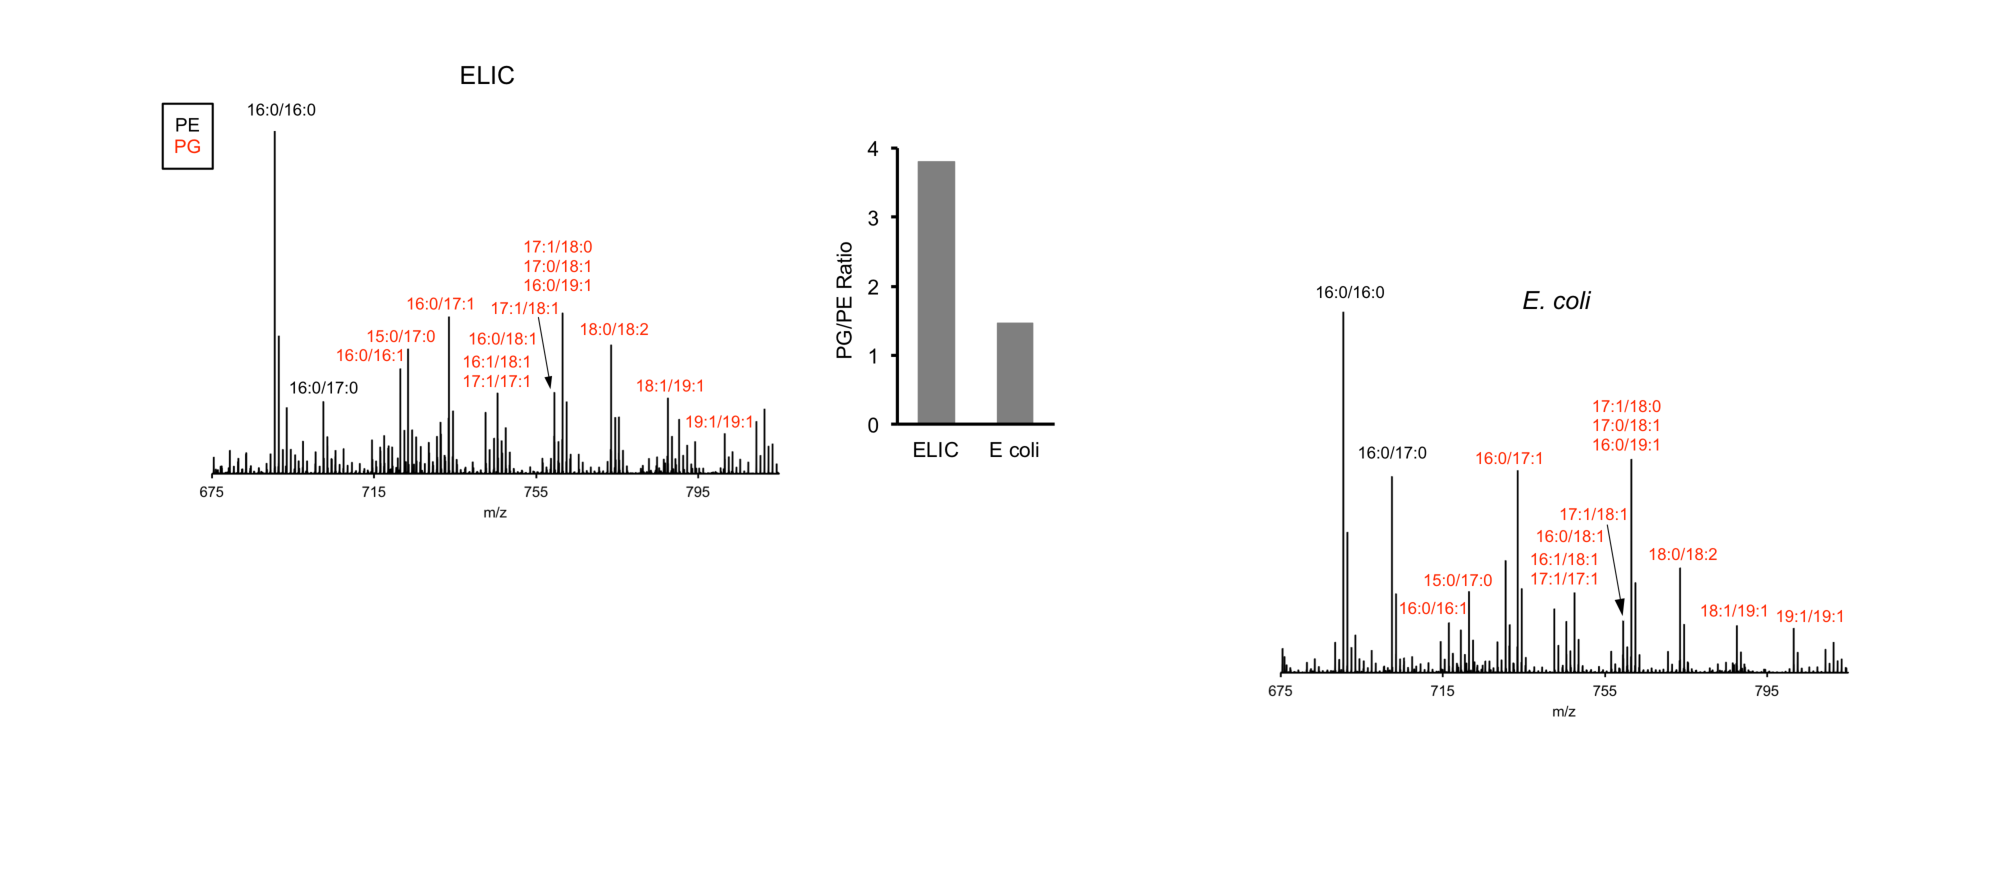
\includegraphics[width=5.95065in,height=3.02741in]{./pandoc_test/media/image11.pdf}
%
%\textbf{Supplementary Fig 1.} MS1 spectra of lipid extract from purified
%ELIC in DDM and \emph{E. coli} membranes. Labeled peaks correspond to PG
%(red) and PE (black) phospholipids with specific acyl chain combinations
%determined from MS2 fragmentation. \emph{Right:} Graph shows
%quantification of the intensity of all PG species relative to PE species
%for ELIC and \emph{E. coli} membrane samples.
%
%\textbf{\\
%}
%
%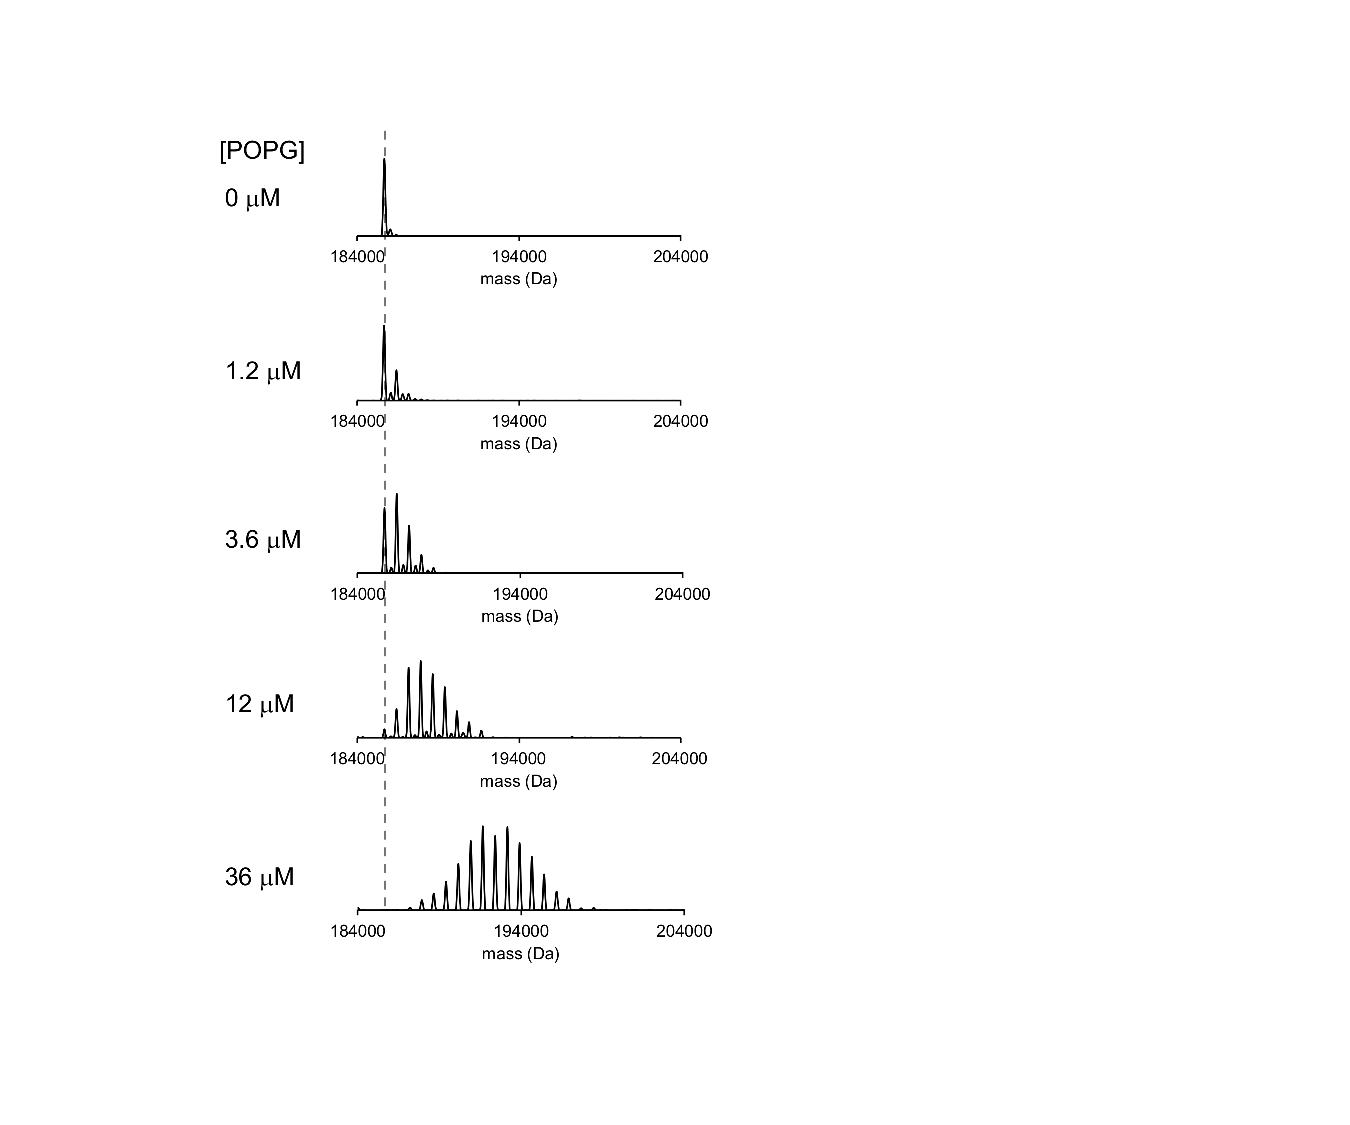
\includegraphics[width=3.18125in,height=5.31611in]{./pandoc_test/media/image12.pdf}
%
%\textbf{Supplementary Fig. \ref{fig:two}.} Representative deconvoluted spectra of 1
%$\mu$M ELIC in C10E5 with increasing concentration of POPG. Dashed line
%indicates mass of apo ELIC.
%
%\textbf{\\
%}
%
%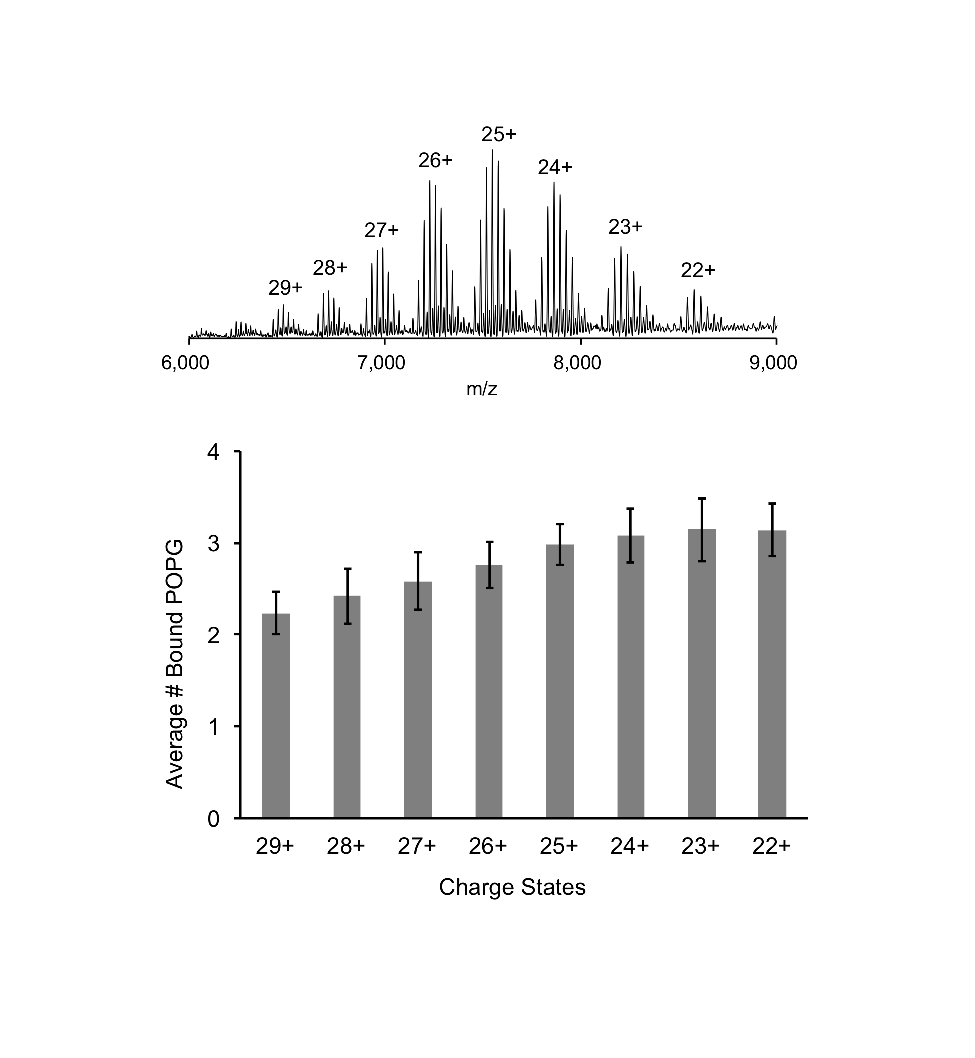
\includegraphics[width=4.64167in,height=5.34307in]{./pandoc_test/media/image13.pdf}
%
%\textbf{Fig. \ref{fig:Supplementary Table 3}.} Comparison of lipid binding at different
%charge states. \emph{Top:} Representative full native spectrum of the
%ELIC pentamer with 12 $\mu$M POPG with each charge state labeled.
%\emph{Bottom:} Quantification of the average number of bound POPG to the
%ELIC pentamer at each charge state (n=13, $\pm$SD).
%
%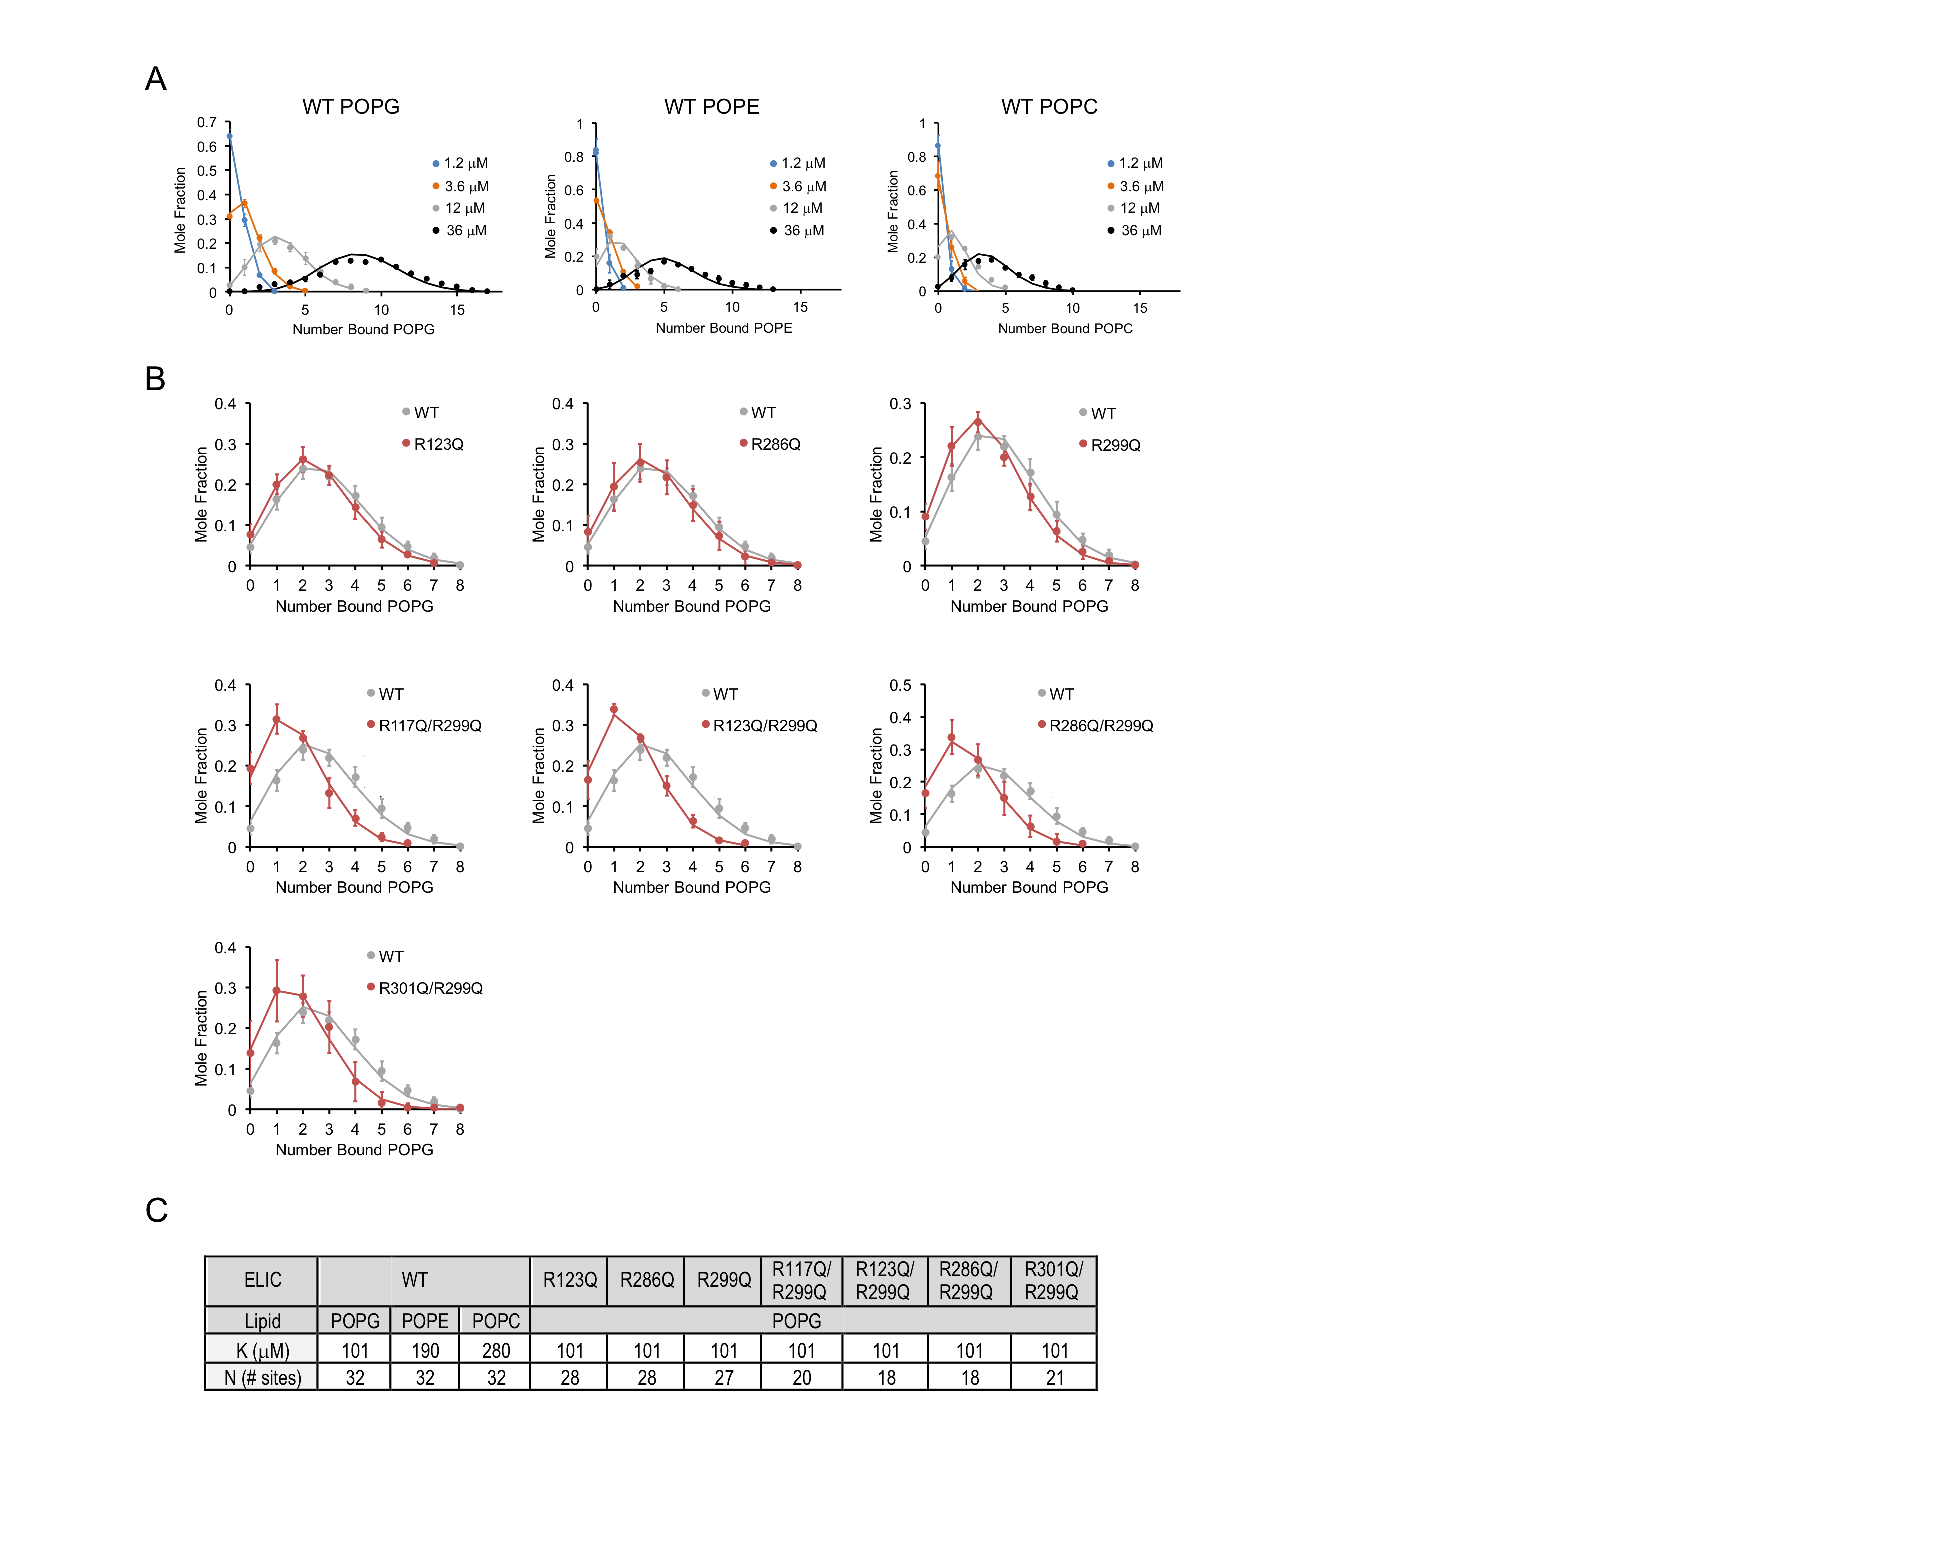
\includegraphics[width=5.51458in,height=7.04808in]{./pandoc_test/media/image14.pdf}
%
%\textbf{Supplementary Fig. \ref{fig:six}.} Lipid binding data fit to binomial
%distributions. (\textbf{A}) Plots of mole fraction of phospholipid-bound
%ELIC derived from native MS experiments with varying concentrations of
%phospholipid (circles, n=3-6, $\pm$SD). Solid lines show global fits from a
%binding model based on a binomial distribution with 32 sites (N) of
%equal affinity (K) using K as shown in (C). (\textbf{B}) Plots of mole
%fraction of POPG-bound ELIC WT and mutants at 12 $\mu$M POPG (circles,
%n=3-6, $\pm$SD). Solid lines show fits as in (A) in which K is held constant
%at 102 $\mu$M and N is varied as indicated in (C). (\textbf{C}) Table
%showing dissociation constants (K) and number of sites (N) used in fits
%shown in (A) and (B).
%
%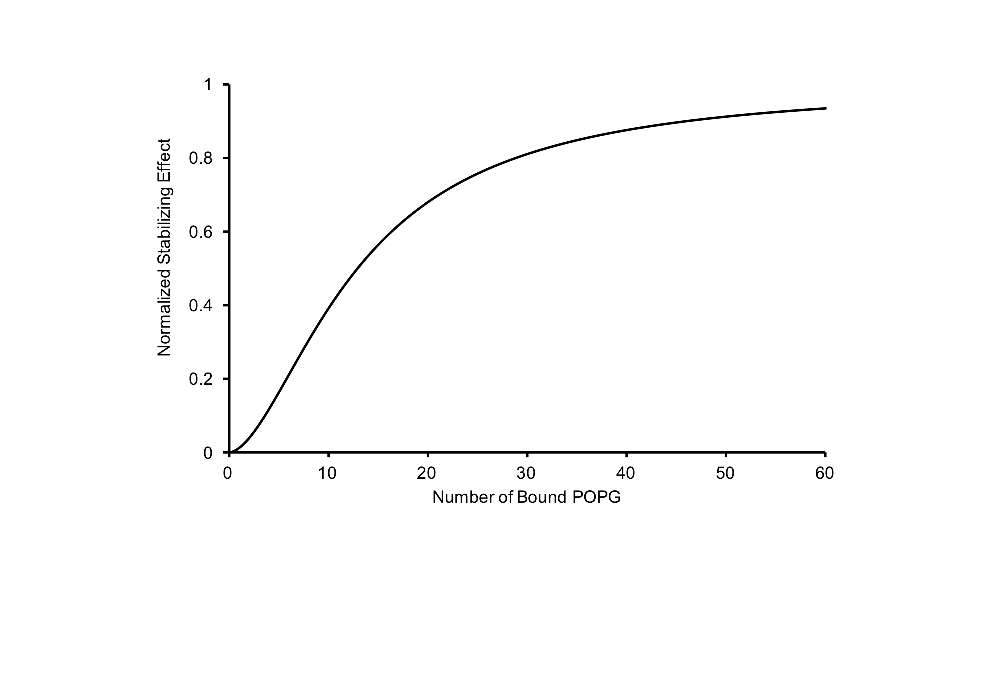
\includegraphics[width=3.93125in,height=2.48554in]{./pandoc_test/media/image15.pdf}
%
%\textbf{Supplementary Fig. \ref{fig:seven}.} Relationship of the thermal stabilizing
%effect of POPG vs the average number of bound POPG derived from equating
%concentration of POPG from the sigmoid functions used to fit the POPG
%binding (Fig. \ref{fig:one}B) and thermal stability data (Fig. \ref{fig:two}A). The resulting
%relationship is: \(S = \ \frac{1}{1 + {(\frac{13.7}{P)}}^{1.7}}\) ,
%where P is the average number of bound POPG and S is the normalized
%thermal stabilizing effect.
%
%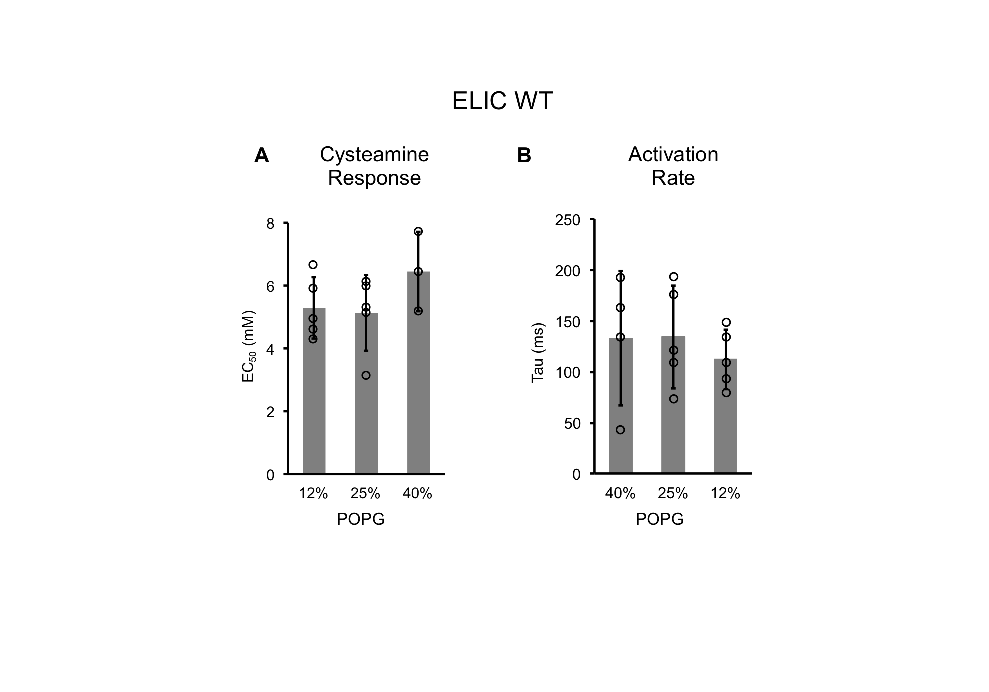
\includegraphics[width=3.67880in,height=3.12778in]{./pandoc_test/media/image16.pdf}
%
%\textbf{Supplementary Fig. \ref{fig:eight}.} Channel properties of WT ELIC responses
%to cysteamine. (\textbf{A}) EC\textsubscript{50} for peak responses to
%cysteamine of WT ELIC in giant liposomes of varying mole\% POPG (n=3-5,
%$\pm$SD). (\textbf{B}) Activation time constants ($\tau$) derived from single
%exponential fits of WT ELIC in response to 30 mM cysteamine in giant
%liposomes of varying mole\% POPG (n=4-5, $\pm$SD).
%
%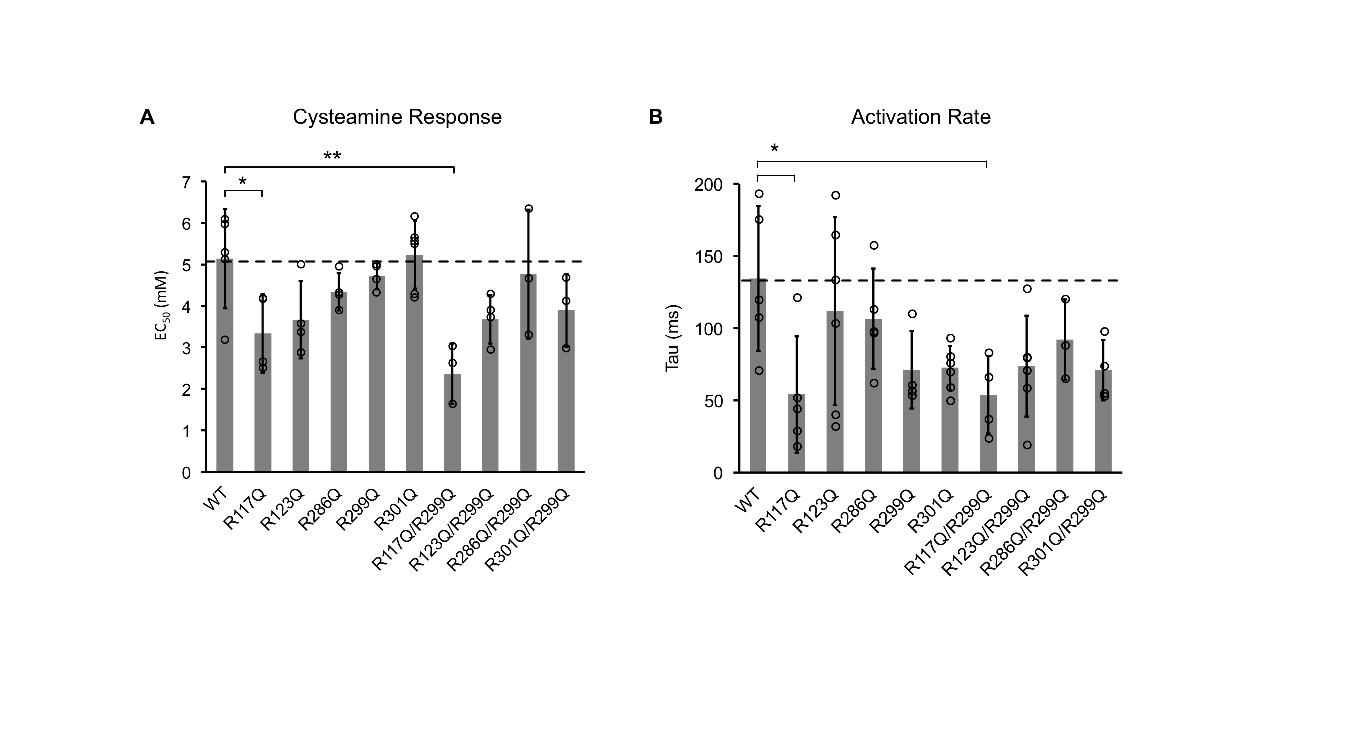
\includegraphics[width=6.43181in,height=3.12778in]{./pandoc_test/media/image17.pdf}
%
%\textbf{Supplementary Fig. \ref{fig:ten}.} Channel properties of ELIC WT and mutant
%responses to cysteamine in giant liposomes of 25 mole\% POPG.
%(\textbf{A}) Graph of EC\textsubscript{50} for peak responses to
%cysteamine of ELIC WT and mutants (n=4-7, $\pm$SD, *p\textless{}0.05,
%**p\textless{}0.01). (\textbf{B}) Activation time constants (tau) of
%ELIC WT and mutants in response to 30 mM cysteamine (n=4-7, $\pm$SD,
%**p\textless{}0.01).
%
%\end{document}

\chapter{Nicotinic Acetylcholine Receptor Boundary Lipid Characterization Within Native and Experimental Membranes}
Pre-print https://arxiv.org/abs/2102.02131\\ \\

\section{Abstract}
The nicotinic acetylcholine receptor (nAChR) and other pentameric ligand-gated ion channels (pLGICs) are native to neuronal membranes with an unusual lipid composition. While it is well-established that these receptors can be significantly modulated by lipids, the underlying mechanisms have been primarily studied in model membranes with only a few lipid species. Here we use coarse-grained molecular dynamics (MD) simulation to probe specific binding of lipids in a complex quasi-neuronal membrane. We ran a total of 50 microseconds of simulations of a single nAChR in a membrane composed of 36 species of lipids. Competition between multiple lipid species produces a complex distribution. We find that overall, cholesterol selects for concave intersubunit sites and PUFAs select for convex M4 sites, while monounsaturated and saturated lipids are unenriched in the nAChR boundary. In order to characterize binding to specific sites, we present a novel approach for calculating a ``density-threshold affinity'' from continuous density distributions. We find that affinity for M4 weakens with chain rigidity, which suggests flexible chains may help relax packing defects caused by the conical protein shape. For any site, PE headgroups have the strongest affinity of all phospholipid headgroups, but anionic lipids still yield moderately high affinities for the M4 sites as expected.  We observe cooperative effects between anionic headgroups and saturated chains at the M4 site in the inner leaflet. We also analyze affinities for individual anionic headgroups. Combined, these insights may reconcile several apparently contradictory experiments on the role of anionic phospholipids in modulating nAChR.
%The nicotinic acetylcholine receptor (\nachr ) and other pentameric ligand-gated ion channels (\plgic s) are native to complex neuronal membranes with an unusual lipid composition. While it is well-established that these receptors can be significantly modulated by lipids, the underlying mechanisms have been primarily studied in model membranes with only a few lipid species.  Here we use coarse-grained molecular dynamics (MD) simulation to test whether specific binding sites observed within model membranes are recovered for a complex quasi-neuronal membrane. We ran a total of 50 microseconds of simulations of a single \nachr{} in a membrane composed of 36 species of lipids. %, including heteroacidic and homoacidic lipids, multiple chain lengths and unsaturation sites, multiple neutral and anionic phospholipid headgroups, and cholesterol.   at the concave intersubunit interfaces as well as convex sites around the M4 helix
% Competition between multiple lipid species produces a complex distribution. We find that overall, cholesterol selects for concave intersubunit sites and PUFAs select for convex M4 sites, while monounsaturated and saturated lipids are unenriched in the \nachr{} boundary. %While those results are consistent with our previous observations from model membranes,  
% In order to characterize binding to specific sites, we present a novel approach for calculating a ``\newaffinity'' from continuous density distributions. The \newaffinities{} reveal a monotonic weakening of affinity with acyl chain rigidity, which is consistent with our previous hypothesis that flexible chains are important for relaxing the packing defects caused by the conical star-shaped \nachr{}.
%We observe that cholesterol selects for intersubunit sites , as expected from model membranes, but has a relatively strong affinity for M4 sites as well. Conversely, neutral n-3 PUFAs are most favorable at M4 sites as expected,  but also successfully competed with cholesterol and saturated lipids for intersubunit sites. 
%For any site, PE headgroups have the strongest affinity of all phospholipid headgroups, but anionic lipids still yield moderately high affinities for the M4 sites as expected. Interestingly, we observe cooperative effects between anionic headgroups and saturated chains at the M4 site in the inner leaflet.  Combined, these insights may reconcile several apparently contradictory experiments on the role of anionic phospholipids in modulating \nachr.     % In model membranes \nachr~is functionally dependent on cholesterol and are modulated by anionic lipids. We showed previously that 1) \nachr~preferentially interacts with long acyl-chained and highly unsaturated polyunsaturated fatty acids (PUFAs) over shorter chained and less saturated PUFAs. 2) \plgic~inter-subunit and M4 have lipid specificity for raft forming lipids and PUFAs, respectively, with anionic lipids favoring sites with more cationic amino acids.  \nachr~boundary lipids in a native neuronal membrane are unknown. Using coarse grained molecular dynamics we simulate \nachr~embedded in a neuronal phospholipid membrane and analyze boundary lipids distribution and using a new approach for calculating binding affinities ($\Delta G$) predict \nachr~neuronal boundary lipid distributions. Cholesterol and neutral n-3 PUFAs had the strongest occupancy affinities of lipids simulated but had the strongest affinities for inter-subunit and M4 sites respectively. Anionic lipids were energetically unfavorable at the TMD in the outer leaflet but had the strongest affinities for inner M4 sites independent of acyl-chain or head group size. 
%We hypothesize lipid-protein occupancy sites where 1) PUFAs, and raft forming lipids would occupy around the M4 and inter-subunit sites respectively. 2) anionic lipids would occupy an inter-subunit region of \nachr~ in the inner leaflet. We analyze 20 potential lipid-protein occupancy sites through $\Delta G$ free energy calculations.

%\begin{keyword}
%%% keywords here, in the form: keyword \sep keyword
%%Jake the Dog \sep Finn the Human
%Neuron \sep \nachr \sep pLGIC \sep PUFAs \sep Cholesterol \sep Ion Channel \sep DHA \sep Affinity Calculation
%%% MSC codes here, in the form: \MSC code \sep code
%%% or \MSC[2008] code \sep code (2000 is the default)
%
%\end{keyword}
%\end{frontmatter}

%%
%% Start line numbering here if you want
%%

%% main text
\section{Introduction}
\label{Intro}

The nicotinic acetylcholine receptor (\nachr)~is a well studied excitatory pentameric ligand gated ion channel (\plgic s). \nachr s are found at high density in post-synaptic membranes and the neuromuscular junction in mammals, and the electric organ in \textit{Torpedo} electric rays. The \nachr~is activated by the binding of agonists such as nicotine or acetylcholine to the orthosteric site in the extra-cellular domain (ECD). When post-synaptic \nachr s are activated {\it en-mass} they stimulate an action potential. Thus \nachr s~play a critical role in both cognition and memory\cite{Henault2015} and neuromuscular function \cite{Mukhtasimova2016,Kalamida2007}. \nachr~ and the greater \plgic~superfamily play various roles in neurological diseases related to inflammation \cite{Taly2009,Patel2017,Yocum2017,Egea2015},  addiction \cite{Cornelison2016}, chronic pain \cite{Xiong2012}, Alzheimer's Disease \cite{Walstab2010,Picciotto_Neuroprotection_2008,MartinRuiz_4_1999,Kalamida2007},spinal muscular atrophy \cite{Arnold_Reduced_2004}, schizophrenia \cite{Haydar2010,Kalamida2007} and neurological autoimmune diseases \cite{Lennon_Immunization_2003, Kumari2008}.
%Egea2015

\nachr s~are highly sensitive to their local lipid environment. \nachr~ poorly conducts ions in model phosphatidylcholine (PC)-only membranes, but can conduct a current with the addition of cholesterol or anionic lipids \cite{Baenziger2017,Dalziel1980,Ellena1983,M.CriadoH.Eibl1982,Fong1986,Fong1987,Jones1988,Sunshine1994,DaCosta2009b,Baenziger2017}, though too much  cholesterol can also cause a loss of function \cite{M.CriadoH.Eibl1982,Mantipragada2003,Barrantes2010a,Baier2011a}. %Barrantes2014
%\grace{LMS There are more examples of this, check Barrantes papers from aughts}  
Functional studies using \xo~ \cite{Zhou2003,Gamba2005,Chen2015,Kouvatsos2016,Nys2016,Polovinkin2018,Moffett2019,Kumar2020} require lipid additives such as asolectin\cite{M.CriadoH.Eibl1982,Zhou2003,Gamba2005,Chen2015,Nys2016,Polovinkin2018,Moffett2019,Kumar2020} or lipids from synaptic membranes \cite{Conti2013} to recover native levels of \nachr{} ion flux.  %This suggests 1) \nachr{} requires more than lipid diversity for native function, and 2) \nachr{} has specific boundary lipids required for native function not found in \xo or there are not enough of these specific lipids to play a boundary role.  
Understanding the mechanism of modulation requires understanding how and where the modulating lipid interacts with the receptor, and these interactions may themselves be dependent upon the rest of the lipid composition.  
%\grace{LMS we don't know the boundary composition, at all, remember? Please unpack/fix this sentence like you did for similar sentences in your thesis.} %lipid composition are essential to function in model membranes or its native neuronal membranes.%Why using addition membranes to restore function rather than cholesterol or anionic lipids is unclear \liam{not quite}. 

Mammalian neuronal membranes \cite{Isolated1969, Taguchi2010, Breckenridge1973,Ingolfsson2017b} have unique compositions compared to other mammalian membranes\cite{McEvoy2000,Kim2001,VanMeer2010,Lorent2020,Ingolfsson2014}. Neuronal membranes are more similar to the membrane of the \textit{Torpedo} electric ray's electric organ \cite{Barrantes1989a,Quesada2016} than the average mammalian membrane\cite{Ingolfsson2014}. The neuronal membrane \cite{Isolated1969, Taguchi2010, Breckenridge1973,Ingolfsson2017b} is rich in lipids in which one or both chains are polyunsaturated fatty acids (PUFAs), particularly the $n-6$ PUFA arachidonic acid (AA), and the $n-3$ PUFAs docosahexaenoic acid (DHA) and eicosapentaenoic acid (EPA). These three PUFA's comprise $\sim20-25\%$ of the acyl chains of neuronal phospholipids, and are involved in secondary signaling \cite{McNamara2006,McNamara2008} and neuronal development \cite{Maekawa2017}. PUFAs are linked to a number of neurological diseases and disorders that overlap \nachr~related diseases. PUFAs play a roll in major depressive and bipolar disorder \cite{Adibhatla2007,McNamara2008,Schneider2017,Koga2019,Hamazaki2015}, schizophrenia \cite{Peet2003,Bushe2005,Berger2006,Schneider2017,Maekawa2017,Hamazaki2015}, and Alzheimer's Disease \cite{Conquer2000,DiPaolo2011,Bennett2013,Adibhatla2007,Yadav2014,Escriba2017}. %Unfortunately, the composition and \liam{microscopic properties} affect on embedded \plgic s is poorly understood.

Functional experiments have focused on the role of anionic lipids and cholesterol as modulators of \plgic s  \cite{Ellena1983,Fong1986,Fong1987,Jones1988,Sunshine1994,DaCosta2009b,Dalziel1980,Addona1998,M.CriadoH.Eibl1982} (the role of polyunsaturation has received comparatively little attention due to common challenges with oxidation of polyunsaturated chains). Such experiments have been overwhelmingly consistent with a role for direct binding of lipids as a modulatory mechanism.   %However, functional experiments cannot determine if lipids directly interact with a protein or determining lipid-protein interaction sites.
As for most membrane proteins, it is experimentally challenging to capture the boundary lipid composition of \plgic~because lipids are small molecules that may remain partly fluid even in their bound state. Numerous structures of \plgic s have revealed a conserved arrangement for both the TMD and the ECD. In the TMD, each subunit has four membrane helices (M1-M4) with the five subunits forming a ``star'' shape around a central pore (Figure \ref{fig:PBT}A). The M2 helix lines the pore, the M1 and M3 helices form a middle ring that includes the intersubunit cavities, and the M4 helices form the tip of the star.  Structural methods have resolved potential cholesterol molecules\cite{Laverty2017, Budelier2019} and phospholipids \cite{Basak2017, Henault2019, Kim2020} bound to subunit interfaces, but crystallographic disorder introduced by lipids typically precludes identification of lipid species. Mass spectrometry has revealed specific binding of anionic lipids, with additional mutagenesis studies suggesting localized sites in the inner leaflet near the M4 helices. \cite{Tong2019} %However, determining structures using cryo-EM or x-ray crystallography, requires ``solid'' structures for imaging. Unfortunately lipids take on multiple conformation due to their fluid nature, resulting in crystallographic disorder, preventing lipid identification.

Molecular dynamics (MD) simulations are particularly useful for visualizing and characterizing microscopic interactions within a fluid system. Given a putative cholesterol or lipid binding mode, atomistic simulations can be used to probe stability of the lipid binding mode.  For pentameric channels, such approaches have primarily demonstrated stability of bound cholesterol\cite{Brannigan2008}, particularly at intersubunit sites\cite{Laverty2017,Henin2014a}.  Unfortunately, fully atomistic simulations suffer from slow diffusion of lipids within the membrane, which prevents spontaneous lipid sorting by proteins over accessible simulation time scales. 

Coarse-grained MD simulations use simplified molecular models that can reveal spontaneous lipid sorting, domain formation, and protein partitioning over simulation timescales \cite{Domanski2012,Chavent2016,Carpenter2018,Ingolfsson2020}. Coarse-grained MD simulations have been used previously to probe interactions of \plgic s with propofol\cite{Joseph2016} as well as spontaneous lipid binding in model membranes\cite{Sharp2019,Woods2019,Tong2019}.  
%\liam{specializes in molecular sized structures, fluids, and predicting structural significance of bound lipids.} 
In previous work, we found that \nachr~embedded in multiple domain-forming model membranes partitioned to the PUFA-rich liquid disordered domain\cite{Sharp2019}, rather than to the cholesterol-rich liquid-ordered or ``raft'' domain that was suggested by cholesterol modulation.  We observed that cholesterol still occupies embedded sites on the \nachr{} TMD, where it is shielded from the liquid disordered domain. However, native membranes are primarily composed of heteroacidic lipids with two distinct chains, where each chain has a different domain preference; such lipids will naturally destabilize domains. In non-domain forming model membranes composed of heteroacidic lipids, two classes of five-fold symmetric sites emerged: an intersubunit site and the M4 site (Figure \ref{fig:PBT}B).  Cholesterol and saturated chains were enriched at the~inter-subunit interfaces and n-3 PUFA acyl-chains were enriched around the M4 helices\cite{Woods2019}. These results were consistent with binding to minimize packing defects: the rigid lipids could fill in the concave regions at the intersubunit sites while the flexible chains would easily deform around the ``star points'' of the M4 helices.  Yet it was not clear whether these same patterns would be upheld in the more complex environment of a native neuronal membrane, which has many more options for minimizing any packing defect.  

Neuronal membranes also contain a sizeable fraction of anionic lipids in the inner leaflet\cite{Isolated1969,Breckenridge1973,Taguchi2010}. With collaborators in the Cheng lab, we recently\cite{Tong2019} showed that anionic headgroups bind preferentially to the \plgic{} Erwinia ligand-gated ion channel (ELIC), when the same acyl chains are used for both headgroups.  Through coarse-grained MD, we found specific binding sites for 1-palmitoyl-2-oleoyl phosphatidylglycerol POPG in the intersubunit sites (inner leaflet); these sites contained basic amino acids that were also implicated through mutagenesis\cite{Tong2019}.  In \nachr{} the high-density of basic amino acids are in the M4 site (inner leaflet) rather than the intersubunit site (inner leaflet), so we would expect a shift for \nachr{} even in model membranes, due purely to the protein sequence. %In neuronal membranes, however, anionic and neutral headgroups do not have the same acyl chain distribution\grace{LMS is this right?} and 
The relative roles of headgroup charge {\it vs} acyl chain saturation in driving affinity are unknown. %Neuronal membranes contain neutral and anionic PUFAs and cholesterol, and we expect: cholesterol to occupy inter-subunit sites in both leaflets. Neutral PUFAs to occupy M4 sites in both leaflets. Simulations of lipid binding revealed spontaneous binding of cholesterol for inter-subunit sites, as well as PUFAs at M4 sites\cite{Woods2019}, as well as anionic lipids binding at inner inter-subunit sites \cite{Tong2019}. 

The use of complex quasi-realistic membranes in coarse-grained MD simulations is growing more feasible. In 2014, Ing{\'o}lfsson et al\cite{Ingolfsson2014} simulated an ``average mammalian'' membrane containing 63 lipids species, followed in 2017 by a coarse-grained neuronal membrane \cite{Ingolfsson2017b}. Multiple accessible and realistic membranes have been developed for comparison of protein-lipid interactions between model and quasi-native membranes\cite{Marrink2019,Wilson2020,Ingolfsson2020,Carpenter2018,Lorent2019}. To our knowledge, no such coarse-grained MD simulations using quasi-native membranes have been used with \plgic s.
% \liam{Based on our previous work \cite{Sharp2019, Woods2019, Tong2019}, we hypothesize a series of lipid occupancy sites for \nachr~based on acyl-chain saturation and head group charge, see Figure \ref{fig:trj}a. We predict PUFAs will occupy regions around the M4 alpha-helices, and raft forming lipids will occupy inter-subunit sites. Neutral lipids are predicted to occupy any site in the outer leaflet and inner leaflet inter-subunit sites, but anionic lipids will predominately occupy only the inner leaflet M4 sites, where there is a higher number of cationic amino acids.}

%The previous model membranes are significantly simplified compared to realistic membranes, i.e. 2-3 lipid species versus 10 or more. 
While the model membranes we used previously are useful for identifying putative sites, they have critical limitations.  As stated previously, model membranes typically vary headgroup charge or acyl chain saturation, not both. Model membranes also do not allow for identification of more specific chemical variations within general saturation classes (i.e. n-3 PUFAs like DHA {\it vs} n-6 PUFAs like $\alpha$-linolenic acid) or like-charged head groups (PC {\it vs} PE, or phosphoserine (PS) {\it vs} phosphoinositol (PI)). For this work, we embed the neuromuscular \nachr\cite{Unwin2005} in a coarse-grained neuronal membrane \cite{Ingolfsson2017b}. To test whether the predictions we developed from model membranes hold for native membranes, we develop a new method for quantifying affinities for partially-occupied binding sites.%Predicting \nachr's native boundary lipid composition is critical to understanding the receptor's function, and what lipid additives are required to mimic a native membrane.

 The remainder of this paper is organized as follows. Section II presents our simulation and analysis approach, including introduction of the \newaffinity.  Section III presents results and discussion of site selectivity of neutral lipids, followed by a reoriented discussion of the same data that is focused on lipid preferences of individual sites. We then consider selectivity of anionic lipids in the inner leaflet and finally consider the effects of specific headgroup differences.  Section IV concludes.  
% This is good stuff, move to abstract: While we had expected that cholesterol would select for intersubunit sites, we found that in neuronal membranes cholesterol had relatively strong affinities for M4 sites as well. Similarly, neutral n-3 PUFAs were most favorable at M4 sites (as in model membranes), but were more commonly found in intersubunit sites than we observed in model membranes. As expected, we observed that in the outer leaflet, neutral lipids were favored while anionic lipids were highly unfavorable. Finally, while we expected that anionic lipids with PUFA chains would have the strongest affinity for M4 sites in the inner leaflet, the charged headgroup dominated the affinity for this site and acyl chain made little contribution.  

%We find our hypothesis, based on model membranes, does not hold. For neutral lipids, inter-subunit sites in both leaflets had strongest affinity for cholesterol. M4 sites had the strongest affinity for neutral PUFAs, though n-3 PUFAs were more favorable than n-6 PUFAs. M4 sites in the inner leaflet had the strongest affinity for all anionic lipids. Saturated and monounsaturated lipids were generally unfavorable. 
% \liam{Neutral lipids are more favorable in the outer leaflet, but n-3 PUFAs and cholesterol tend to occupy \nachr~sites indiscriminately. In the inner leaflet neutral n-3 PUFAs and cholesterol tend to compete with anionic n-3 PUFAs and cholesterol tend to occupy inter-subunit sites, but anionic lipids occupy M4 regardless of acyl-chain saturation.}

\section{Methods}
\label{lab}

\subsection{Simulation Composition}
All simulations used the coarse-grained MARTINI 2.2\cite{DeJong2012} topology and forcefield.
\nachr~ coordinates were based on a cryo-EM structure of the $\alpha{\beta}\gamma\delta$ muscle-type receptor in native torpedo membrane (PDB 2BG9\cite{Unwin2005}). This is a medium resolution structure (4\AA) and was further coarse-grained using the martinize.py script; medium resolution is sufficient for use in coarse-grained simulation, and the native lipid environment of the proteins used to construct 2BG9 is critical for the present study. The secondary, tertiary and quaternary structure in 2BG9 was preserved via soft backbone restraints during simulation as described below, so any inaccuracies in local residue-residue interactions would not cause instability in the global conformation.  

\nachr~was embedded in a coarse-grained neuronal membrane based on Ing{\'o}lfsson et al\cite{Ingolfsson2017b}. The neuronal membrane from described by Ing{\'o}lfsson contains phospholipids, sterols, diacylglycerol, and ceramide. Membranes presented in this paper only consider phospholipids and cholesterol, for a total of 36 unique lipid species, see Table \ref{tab:rats}.

Coarse-grained membranes were built using the MARTINI script insane.py \cite{Wassenaar2015}, which was also used to embed the coarse-grained \nachr~within the membrane. The insane.py script randomly places lipids throughout the inter- and extra-cellular leaflets, and each simulation presented in this manuscript was built separately. All simulation box sizes were $40x40x35$ nm$^3$ with  $\sim 4,500-5,000$ lipids and total $\sim450,000$ beads.

\subsection{Simulations}

Molecular dynamics simulations run using the MARTINI 2.2\cite{DeJong2012} forcefield and GROMACS\cite{Berendsen1995,Abraham2015}  2019.2 . All systems used van der Waals (vdW) and Electrostatics with reaction-field and a dielectric constant of $\epsilon_r$=15 and electrostatic cutoff length at 1.1 nm. Energy minimization was performed for 1000000 steps, but energy minimization tended to concluded after $\sim 5000-10000$ steps.

Volume and pressure equilibrations were run with isothermal-isochoric (NVT) and isothermal-isobaric (NPT) ensembles respectively. NVT and NPT simulations used a time step of 15 fs and run for 0.3 ns using Berendsen thermostat held at a temperature of 323 K, and Berendsen pressure coupling with compressibility set to 3$\times$10$^{-5}$ bar$^{-1}$ and a pressure coupling constant set to 3.0 ps  for the NPT ensemble. 

Molecular dynamics simulations were run using a time step of 20 fs for 5 $\mu$s for 10 replicas. Simulations were conducted in the NPT ensemble, by using the velocity rescaling to a temperature of 323 K with a coupling constant set to 1 ps. Semi-isotropic pressure coupling was set to Parrinello-Rahman with compressibility at 3$\times$10$^{-5}$ bar$^{-1}$ and pressure coupling constant set to 3.0 ps. 

Secondary structures restraints with MARTINI recommendations were constructed by the martinize.py \cite{DeJong2012} script and imposed by GROMACS \cite{Berendsen1995,Abraham2015}. The \nachr~conformation was preserved by harmonic bonds between backbone beads separated by less than 0.5 nm and calculated using the ElNeDyn algorithm \cite{Periole2009} associated with MARTINI \cite{DeJong2012} with a coefficient of 900 kJ$\cdot$mol$^{-1}$.
\begin{figure*}[!h]
	\center
	%\includegraphics[width=\linewidth]{PartialBIndingToy.pdf}
	\includegraphics[width=\linewidth]{./Figures/PartialBIndingToy.pdf}
	\caption[ Binding site boundaries and distribution definitions.] { (a) Structure of the \nachr {}TMD\cite{Unwin2005}, viewed from the extracellular domain. Helices are colored by subunit ($\alpha$:green, $\beta$:purple, $\gamma$: cyan, $\delta$:grey). (b) Boundaries of the pseudo-symmetric intersubunit (black) and M4 (white) sites. The angular components are determined by the location of the M1 and M3 alpha-helices for either two adjacent subunits (intersubunit sites) or a single subunit (M4 sites), and are listed in Table S5. Circles correspond to the helices shown in panel A.  (c)  The distributions $P_{site} (n)$ (blue) and $P_{bulk}(n)$ (dashed red) represent the probability distributions for number of beads of a certain lipid species in the site or in an analogously-sized area of the bulk, respectively. The value $n_{peak}$ maximizes $P_{bulk}$. $P_<$ (pink) is the area under $P_{site}$ to the right of $n_{peak}$ while $P_>$ (light blue) is the area under $P_{site}$ to the right of $n_{peak}$. }
	\label{fig:PBT}
\end{figure*}

\subsection{Calculation of Polar Density Distributions}
As in our previous work\cite{Sharp2019, Woods2019, Tong2019}, the two-dimensional density distribution $\rho_{B}$ of the beads within a given lipid species $B$ around the protein was calculated on a polar grid:
  \begin{equation}
      \rho_{B}(r_i,\theta_j)= \frac{\left\langle n_{B}(r_i,\theta_j) \right\rangle}{r_i \Delta{r}\Delta{\theta}} \\        
    \label{eq:R}
  \end{equation}
  where  $r_i = i \Delta{r}$ is the projected distance of the bin center from the protein center, $\theta_j = j \Delta{\theta}$ is the polar angle associated with bin j,  $\Delta{r}$= 10\AA~ and  $\Delta{\theta} = \frac{\pi}{15}$ radians are the bin widths in the radial and angular direction respectively, and $\left\langle n_{B}(r_i,\theta_j) \right\rangle$ is the time-averaged number of beads of lipid species $B$ found within the bin centered around radius $r_{i}$ and polar angle $\theta_{j}$.  In order to determine enrichment or depletion, the normalized density $ \tilde{\rho}_{B}(r_i,\theta_j)$ is calculated by dividing by the approximate expected density of beads of lipid type B in a random mixture, $x_{B}s_{B}~N_{L}/\langle L^{2}\rangle$, where $s_{B}$ is the number of beads in one lipid of species B, $N_{L}$ is the total number of lipids in the system, and $\langle L^{2}\rangle$ is the average projected box area:
  \begin{equation}
  \tilde{\rho}_{B}(r_i,\theta_j)=\frac{ \rho_{B}(r_i,\theta_j)}{x_{B}s_{B}~N_{L}/\langle L^{2}\rangle} \\        
    \label{eq:Rt}
  \end{equation}
where the expected density is derived at the first frame of the simulation. Python software for these calculations are under active development and are located at \cite{2Dgithub}.  
 
This expression is approximate because it does not correct for the protein footprint or any undulation-induced deviations of the membrane area.  The associated corrections are small compared to the membrane area and would shift the expected density for all species equally, without affecting the comparisons we perform here. For a given lipid species or class, analysis excluded any replicas in which fewer than 5 lipids of the species/class were in the leaflet at any point in the sampled simulation.
 %\grace{LMS:Previous sentence is woefully insufficient.  How did you get the distributions of the number of beads per site? (i.e. Was it a distribution across frames? Or across sites? How did you determine the number of beads in a site each frame? How frequently did you sample? } For the affinity calculation described above the bin radial and angular widths are $\Delta r=$  4$\AA$ and $\Delta \theta=$ $\frac{\pi}{25}$.\grace{LMS: I moved this sentence up here because the information fits here, but it needs to be adjusted to fit with this section}

 \subsection{Calculation of the \newaffinity}
 
Although lipids to occupy clearly detectable hot-spots, binding to these sites are not straightforward to describe by a traditional two-state model. Lipids are chains that may partially occupy or fully occupy a site, and they may share a site with another lipid that is partly or fully occupying the site.  While the standard affinity can be determined from the probability of single occupancy, the \newaffinity{} is determined from the probability that a site is occupied by more beads than would be expected based on bulk density. %instead we consider partial occupation. Partial occupancy ranges from fully occupied, partially occupied, or unoccupied. A site is fully occupied if a single lipid species (A) is the only lipid species occupying a site. Like the small molecule displaced by water, a portion of lipid A may be partially or fully displaced by a second lipid (B). 

%A traditional affinity reflects the free energy difference between an occupied and unoccupied state, where we consider the free energy difference between enriched density in the site and depleted density in the site.  

For a given site, consider %Free energy calculations are defined as the change in the Gibbs' free energy ($\Delta G$). $\Delta G$ is calculated using 
two probability distributions: the probability $P_{site}(n)$ of finding $n$ beads within the site and the probability $P_{bulk}(n)$ of finding $n$ beads within a region of equivalent area in the bulk, respectively.   For a lipid that has no affinity for this binding site, we expect $P_{site}(n) = P_{bulk}(n),$ while $P_{site}(n)$ should be right-shifted for a strong affinity and left-shifted in the presence of competition. %\grace{LMS please notice that I have changed $P_{occ}$ to $P_{site}$ because it contrasts better with $P_{bulk}$. This will need to be changed in any figures.} %Both distributions are calculated from the time averaged number of lipid beads within the area of an occupancy site ($P_{occ}$) or an identical area in the bulk membrane ($P_{bulk}$).  
We calculate the degree of right or left shift by first finding the number of beads $n_{peak}$ that corresponds to the peak of the density distribution in the bulk. As illustrated in Figure \ref{fig:PBT} C, we then integrate $P_{site}$ on both the left and right side of the threshold $n_{peak}$ to yield $P_{<}$ and $P_{>}$ respectively:
\begin{eqnarray}
    %P_{<} \equiv \big\{\sum P_{occ} \leq \big< P_{bulk} \big> \big\} \label{eq:Pl} \\
    %P_{>} \equiv \big\{\sum P_{occ} > \big< P_{bulk} \big> \big\} \label{eq:Pg}
    P_{<}& \equiv &\sum\nolimits_{n\le n_{peak}} P_{site}(n) \label{eq:Pl} \\
    P_{>}& \equiv &\sum\nolimits_{n>n_{peak}} P_{site}(n)  \label{eq:Pg}
\end{eqnarray}
Note that this step breaks the distribution into two macrostates on either side of the threshold, allowing clear analogy with a classic binary binding model.  %Using the mean value of $P_{bulk}$ ($ \big< P_{bulk} \big> $) as a reference, the sum of $P_{occ}$ less than or equal to   $\big< P_{bulk} \big> $ is defined as $P_{<}$. The sum of  $P_{occ}$ greater than  $\big< P_{bulk} \big> $ is defined as $P_{>}$. The affinity is then defined as the overlap between $P_{<}$ and $P_{>}$.
The free energy difference between the two macrostates is
\begin{equation}
\Delta G = -RT\ln\frac{P_{>}}{P_{<}}
\label{eq:dG}
\end{equation}
where R is the gas constant and T is temperature. We term this free energy difference the ``\newaffinity''.  In the special case of binary occupancy, 
\begin{eqnarray}
P_{site}(n)&= 
\begin{cases}
    (1+ K_{D}/[L])^{-1},& \text{if } n = 1\\
    (1+ [L]/K_{D})^{-1},& n=0
\end{cases}
\end{eqnarray}
where $K_{D}$ is the dissociation constant and $[L]$ is the ligand concentration. In a dilute solution the volume per ligand is typically much larger than the site volume, so $P_{bulk} (n)=1$ for $n=0$ and vanishes for all $n>0$, so $n_{peak} = 0$. Consequently, for this special case, $P_{<} = (1+ [L]/K_{D})^{-1}$ and $P_{>} = (1+ K_{D}/[L])^{-1}$. 
Then Equation \ref{eq:dG} reduces to the classic form for the chemical potential $RT\ln K_{D}-  RT\ln [L]$. 

\subsection{Binding Site Definition and Occupancy Calculations}

We consider two classes of site: intersubunit sites and M4 sites. Each \plgic~has ten of each site (five in the outer leaflet and five in the lower leaflet) for a total of twenty sites (Figure \ref{fig:PBT}B).  The boundaries for each site were drawn to correspond to the localized binding hot spots observed for heteroacidic membranes\cite{Woods2019}, and are non-overlapping. Inter-subunit sites include bins with angular components between the M1 and M3 alpha-helices of two adjacent subunits, and a radial component satisfying $10<r\leq32$\AA.  M4 sites include bins with complementary angular components (so that no sites overlap) falling within the M1 and M3 alpha-helices of a single subunit, and a radial component satisfying $10<r\leq44$\AA. For a full description of radial and angular dependencies, please see Table \ref{tab:pars}. 

In order to calculate $P_{site}(n)$, a distribution was taken across frames at 10 ns intervals. For any frame, the  beads of a given lipid or chain type were binned onto a fine polar grid with $\Delta r=$  4\AA and $\Delta \theta=$ $\frac{\pi}{25}$. The bins falling within the site boundaries were then summed to calculate the occupancy $n$.  This approach allowed for straightforward adjustment of site boundaries if needed without needing to re-bin the whole trajectory.  % Using the polar density distributions, we isolated specific sites with masks based on the above site limits. For each site, the number of beads of a specific lipid species (or acyl-chain species) were counted every 10$ns$ of the trajectory. %Probability distributions are the number of lipid beads within a given site over 
%Finer bins are required to accurately describe specific sites. Instead radial and angular widths are changed to: 

\subsection{Calculation of Accessible Area}

Calculation of $P_{bulk}$ requires determining the accessible site area in order to calculate the densities in a bulk region of similar area. The area $A$ accessible to the lipids is the difference between the total site area $A_{tot}$ and the area $A_{ex}$ excluded by the protein: $A = A_{tot} - A_{ex}  $
%We are interested in $A_{acc_s}$, which appears in eq \ref{eq:As}. 
$A_{tot}$ is straightforward to calculate by summing over the areas of the bins $i$ within the site boundaries: $A_{tot} = \sum_i r_i \Delta r_i  \Delta \theta_i$.  Calculating $A_{ex}$ is less straightforward, and although there are many possible ways to do this, for self-consistency we used the same tools from our primary analysis.  

In a single lipid membrane, $P_{site}(n)=P_{bulk}(n)$ as long as $P_{bulk}(n)$ is calculated using the proper area $A$.  We exploit this identity to calculate $A$ for each site, by running a single \nachr{} in pure di-palmitoyl phosphatidylcholine (DPPC) for $\sim 370$ns and determining the value of $A$ for each site such that $P_{site}(n)$ and $P_{bulk}(n)$ have the same peak.  These areas are reported in Table \ref{tab:pars}. 
%\begin{equation}
    %A_s = \frac{\left\langle n_s(r,\theta) \right\rangle}{\rho_s(r,\theta)}
%    A_tot = \sum_s r_s \Delta r_s  \Delta \theta_s
%\label{eq:A}
%\end{equation}
%where $\left\langle n_s(r,\theta) \right\rangle$ is the associated time averaged number of beads within a polar bin and $\rho_s$ is the time averaged numeric bin density (eq \ref{eq:R}). \grace{LMS: Why don't we just calculate the bulk area by summing the bin areas? Why do we divide n by rho? This seems really unnecessary.} \liam{Ah, yes, we do what you wrote. What I have is from like... may? } Only values of $\left\langle n_s(r,\theta) \right\rangle$ and  $\rho_s$ within the range of angular and radial bins described above are used. Using the values calculated for $A_s$, we calculate $A_{acc}$ to determine accurate bulk densities for $P_{bulk}$.

%    \begin{equation}
 %   	A_{acc_s} \equiv \frac{\left\langle n_{site_s} \right\rangle A_s }{\left\langle n_s \right\rangle} \label{eq:aac}\\
 %   \end{equation}
    
%    \begin{equation}
 %   	A_{rest_s} \equiv A_s - A_{acc_s} \label{eq:aac}\\
 %   \end{equation}
    
%    $\left\langle n_{site_s}\right\rangle$ and $\left\langle n_s  \right\rangle$ are the average number of lipid beads for a specific occupancy site and the average number of lipid beads in the bulk membrane within a given area $A_s$. The values for $A_{acc_s}$ are then used to calculate $P_{bulk}$, see Figure \ref{fig:PBT} a.
%    \grace{This piece confuses me and I need to understand it better before I can edit.} \liam{I think I should have also had $A_{rest}$, this is to show how we determine the accessible and restricted areas.}

 \begin{figure*}
	\center
	\includegraphics[width=\linewidth]{./Figures/Trajectory.pdf}
	%\includegraphics[width=3in]{Trajectory.pdf}
	\caption[A molecular perspective of coarse-grained simulation results] {. a) Multiple frames from a single simulation replica over 5 $\mu s$.   The \nachr{} TMD is shown in surface representation and colored as in Figure 1. Cholesterol and acyl chains within 15 \AA~ of \nachr{} are shown as beads, and colored by chain type: saturated lipids: blue, monounsaturated lipids:orange, n-6 PUFAs:pink, n-3 PUFAs: beige, and cholesterol: red.  Each phospholipid color includes several lipid species of the same type, and simulations included a larger membrane and the ECD, which is not shown.  b) Representative poses of lipids for individual sites, colored as in A, but viewed from within the membrane looking at the TMD surface. Cholesterol selects for the intersubunit site while monounsaturated lipids have a particularly low affinity for this site. PUFAs select for the M4 site, while saturated lipids have a particularly low affinity.}
	\label{fig:trj}
\end{figure*}

\section{Results and Discussion}
\label{res}

\begin{figure*}[!h]
	\center
	\includegraphics[width=4in]{./Figures/acyl_heatmap.pdf}
	%\includegraphics[width=\linewidth]{acyl_heatmap.pdf}
	%55mm]{acyl_heatmap.pdf}
	\caption[Lipid density enrichment around a central singular \nachr.]  {(a) and (b) Density enrichment $\tilde{\rho}_{a}$ for lipids in a neuronal membrane, calculated using eq \ref{eq:Rt} for both outer and inner leaflets, averaged over 10 replicas for 2.5 $\mu$s each. The maximum radius from the \nachr{} pore is 60 \AA. Depletion relative to a random mixture ($\log\tilde{\rho}_{a}< 0$) is blue while enrichment ($\log\tilde{\rho}_{a}> 0$) is red. Lipids are organized by acyl chain (a) or headgroup (b). Acyl chain density includes only the relevant chain of a heteroacidic lipid, while headgroup density includes the whole lipid.  Helices are represented as circles colored as in Figure 1. Intersubunit (solid line) and M4 (dashed line) site boundaries are marked.  (c) Equivalent analysis for \nachr{} in a model membrane of 2:2:1 n-3 PUFA:saturated:cholesterol, using previously published trajectories\cite{Woods2019}. } 
	 %describes acyl-chain depletion compared to a random bulk mixture, $\tilde{\rho}_{a}=0$ describes the expected mixture, and $\tilde{\rho}_{a}  > 1$ describes acyl-chain enrichment compared to a random mixture. a) Density enrichment based on acyl-chains, b) density enrichment based on head group charge.}
	\label{fig:acyl_map}
\end{figure*}

\subsection{Effect of acyl chain on site selectivity among neutral lipids}

%\textit{SECTION 3.1:  EFFECT OF ACYL CHAIN ON NEUTRAL LIPID AFFINITIES a) Results block for figure 2.  b) Results block for figure 3 (neutral)  c) Results block for figure 4 (neutral). Results blocks in all three cases should be focused on role of unsaturation/chain flexibility.}

%Results from Woods et al 2019 \cite{Woods2019} predict lipid occupancy sites for PUFAs and raft forming lipids at M4 and inter-subunit sites respectively. To test this whether we observe similar behavior in neuronal membranes, we use radial enrichment densities (see eq \ref{eq:Rt}) and calculated affinities as $\Delta G$ values, described in methods and equations \ref{eq:A}-\ref{eq:dG}.

\begin{figure*}[!h]
	\center
	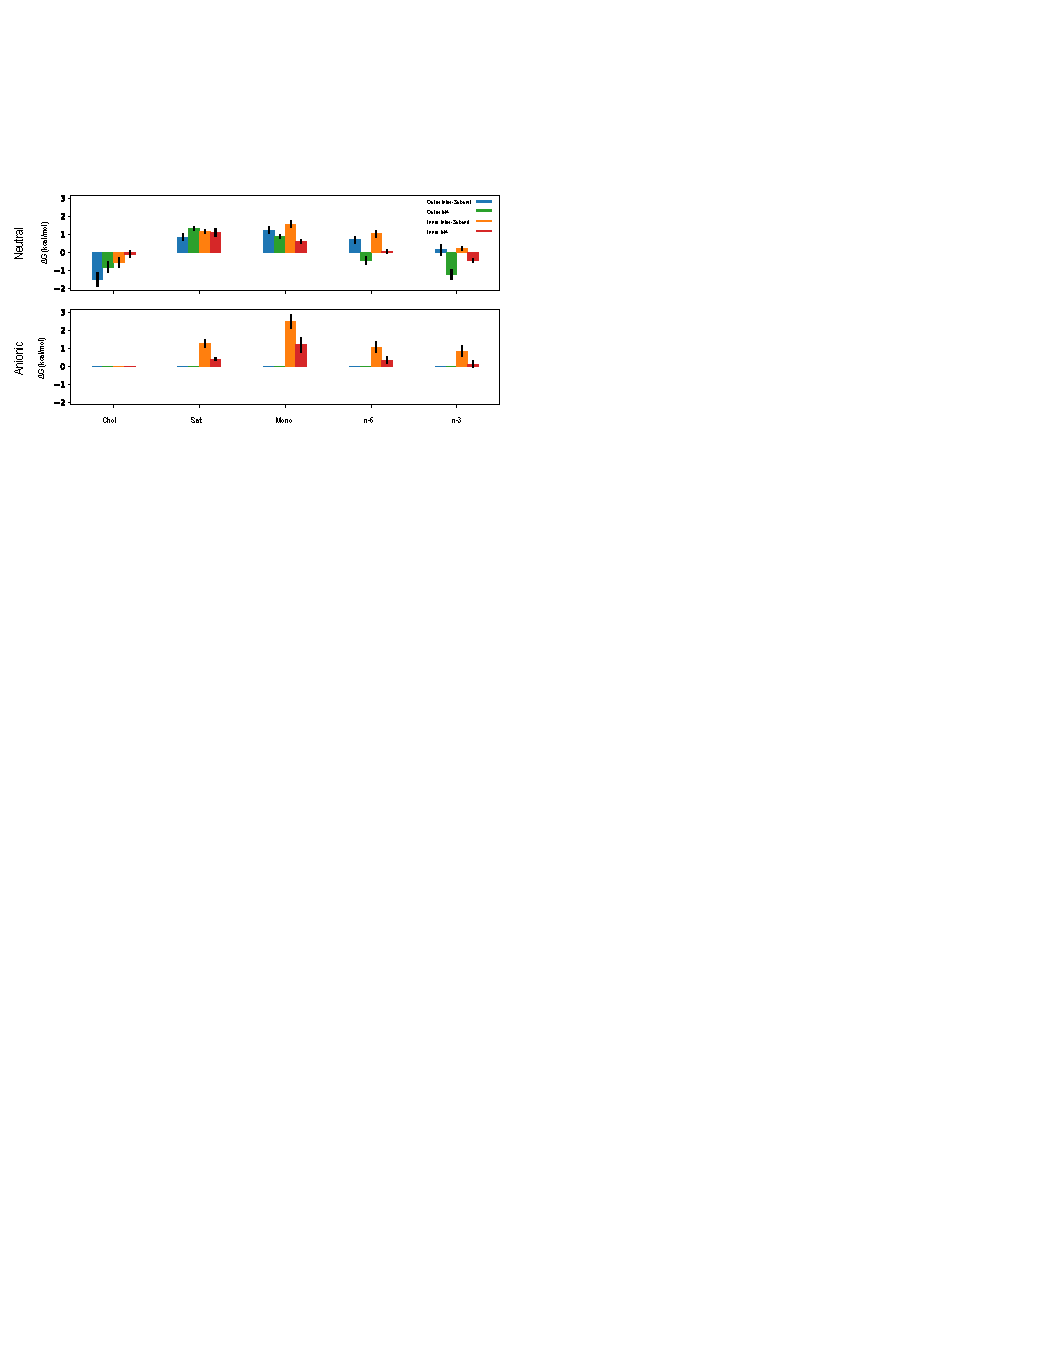
\includegraphics[width=\linewidth]{./Figures/Protein_centric.pdf}
	\caption[\Newaffinities{} organized to reveal site selectivity.] {The \newaffinities ($\Delta G$) are calculated using Equation \ref{eq:dG}, where error bars are the standard error (n=10 independent replicas).  \Newaffinities are colored by site; in the outer leaflet: intersubunit (blue) and  M4 (green), and for the inner leaflet: intersubunit (orange) and M4 (red). Values are separated by headgroup charge (rows) and acyl chain type (columns). More negative values indicate stronger affinities, while more positive values indicate more displacement of the lipid by other lipid species. Data incorporates 10 replicas averaging over the last half of the 5$us$ trajectory, with five-fold averaging over each type of pseudosymmetric site. Figure \ref{fig:lipidBar} has an alternate representation of the same data.  }  % Colors: Outer Inter-Subunit:blue, Outer M4:green, Inner Inter-Subunit:orange, Inner M4:red.}
	\label{fig:proBar}
\end{figure*}

Representative frames from a typical trajectory of boundary lipids are shown in Figure \ref{fig:trj}A, with representative poses shown in Figure \ref{fig:trj}B.  In order to quantitatively compare the lipid distributions for the native system to our previous model system, we plotted the enrichment of boundary density relative to bulk density on a two-dimensional polar heat map centered around the protein. This enrichment is shown in Figure \ref{fig:acyl_map}A for cholesterol and various acyl chains grouped by  saturation. Saturated and monounsaturated acyl chains are not significantly depleted or enriched in the boundary of the protein. Regions of cholesterol density are much more localized than in the model membrane (Figure \ref{fig:acyl_map}C) , with pockets of high enrichment very close to the protein and weak depletion in the remainder of the boundary region.  Both n-6 and n-3 PUFA chains yield five-fold symmetric enrichment around the M4 alpha-helices, as observed for n-3 PUFAs in the model membrane.  In the neuronal membrane, however, this enrichment is less well-defined and spreads into the intersubunit regions. In particular, additional pockets of significant enrichment are apparent in the $\beta-\delta$ subunit interface in the outer leaflet. The overall area of the regions of PUFA-enrichment decrease in the inner leaflet, where n-3 PUFAs are enriched around M4 helices, but n-6 PUFA density is not five-fold symmetric and has weak enrichment. Overall, the loss of definition in site boundaries diverges from the well-defined five fold enrichment for n-3 PUFAs we saw in model membranes\cite{Woods2019}. 

In order to reduce these distributions to affinities that are more straightforward to interpret, we calculated the \newaffinity{}  $\Delta G$ for various lipid species as defined in Eq. \ref{eq:dG}. We organize this information in two different ways: Figure \ref{fig:proBar} provides the ``lipid's perspective'' and is organized to identify the preferred site for a given lipid type (the lipids' ``site selectivity''), while Figure \ref{fig:lipidBar} provides the ``site's perspective'' and is organized to identify the most favorable lipids for a given site (the sites' ``lipid specificity''). 

We first consider site selectivity for neutral lipids. Affinities for neutral lipids and cholesterol are shown in Figure \ref{fig:proBar}A, where more negative values of $\Delta G$ indicate a stronger \newaffinity{} and more positive values indicate more displacement by other lipids.  Overall, as shown in Figure \ref{fig:proBar}A, saturated lipids have similar \newaffinities{} across all sites, which is consistent with the generally flat distribution observed in Figure \ref{fig:acyl_map}. Yet saturated lipids do yield a slightly stronger affinity for intersubunit sites, at least in the outer leaflet, which may drive the high amount of saturated enrichment observed at these sites in model membranes.  Outer leaflet monounsaturated lipids are slightly more unfavorable in intersubunit sites than M4 sites, and this difference grows in the inner leaflet. 

In contrast to saturated and monounsaturated lipids, PUFAs and cholesterol are highly selective for particular sites.  As shown in Figure  \ref{fig:proBar}A, neutral PUFAs have significantly stronger affinities for M4 sites than for innersubunit sites in the same leaflet.  Such selectivity is consistent with the PUFA enrichment density in Figure \ref{fig:acyl_map}A, where n-3 PUFAs can occupy most regions of the TMD but have particularly high levels of enrichment around M4. It is further consistent with our expectations from model membranes (Figure \ref{fig:acyl_map}C). Regardless of the site class, PUFAs favor the outer leaflet site over the inner leaflet site, but both sets of M4 sites are more favorable than both sets of intersubunit sites.  Conversely, cholesterol has significantly stronger affinities for innersubunit sites than for M4 sites, which is also consistent with the enrichment density in Figure \ref{fig:acyl_map}A and our expectations from model membranes (Figure \ref{fig:acyl_map}C). For cholesterol, however, the leaflet is a bigger determinant of affinity than the site; cholesterol has a stronger affinity for either outer leaflet site compared to either inner leaflet site.  

\subsection{Lipid preferences of intersubunit and M4 sites}
We now switch perspectives to considering which neutral lipids are most favorable for particular sites. As shown in Figure \ref{fig:lipidBar} A and B, intersubunit sites in both leaflets prefer cholesterol to phospholipids, which is expected based on the results from model membranes.  Upon visual inspection, this result may appear to diverge from the cholesterol polar density plots in neuronal membranes (Figure \ref{fig:acyl_map} A).  The present results show that while the overall footprint of cholesterol enrichment in (Figure \ref{fig:acyl_map} A) is small, this small region actually reflects a tight and persistently occupied binding site.  The highly right-shifted distributions for cholesterol are shown in Figure S1.  %\grace{LMS: I'm not sure about the following explanation.  Did we discuss this? If so, can we discuss it again? } \liam{we had, though it was my understanding it was roughly the same as what is in the previous sentence.}    We argue difference between weak cholesterol enrichment and strong cholesterol affinity is a result of averaging. For the density analysis, the peak of the the lipid distribution is isolated as a result of averaging, while for the affinity calculation, the full distribution is used to compute the affinity, see Figure SI 1.

PUFA chains yield affinities for the intersubunit site that are approximately $>$0.5 kcal/mol stronger than saturated lipid affinities (Figure \ref{fig:lipidBar} A and B), which was unexpected based on results from model membranes but is consistent with the corresponding enrichment density in Figure \ref{fig:acyl_map}A. More generally, neutral phospholipid affinities for intersubunit sites obey the following trend, from strongest to weakest: n-3 $>$ n-6 $>$ saturated $>$ monounsaturated. Thus, even though PUFA chains prefer M4 sites to intersubunit sites,  and saturated chains prefer intersubunit sites to M4 sites, PUFAs have a stronger affinity for either site type than do saturated lipids. 
 
For intersubunit sites, monounsaturated lipids have the weakest affinities ($>0.5$ kcal/mol), which may reflect a limited number of ways to pack the single kink of a monounsaturated chain in this concave site. In contrast, cholesterol and PUFAs are either small or highly flexible and may more easily pack across multiple sites. Saturated chains may pack parallel to the protein surface in these sites. 
% may pack around inter-subunit site's concave topology. The single acyl-chain kink found in monounsaturated lipids may prevent packing of itself around inter-subunit sites, and is not flexible to compete with PUFA's occupying M4 sites. 

As shown in Figure \ref{fig:lipidBar}C and D, M4 sites in both leaflets have the strongest affinity for n-3 PUFAs, and affinity weakens as acyl chain rigidity increases; from strongest to weakest the phospholipid affinities follow: n-3 $>$ n-6 $>$ monounsaturated $>$ saturated.  This is consistent with a role for PUFAs in minimizing unfavorable membrane deformations caused by the \plgic's conical-star shape.\cite{Brannigan2007,Kim1998,Dan1993,Goulian1996,Goulian1993,Fournier2015}  Surprisingly, cholesterol had a stronger affinity for M4 sites than any acyl chains other than n-3 PUFAs. Cholesterol is rigid, small, and has asymmetric sides (rough and smooth) which potentially allows it to embed between alpha-helices and compete with n-3 PUFAs for binding. Any cholesterol bound within the grooves of the subunit interface (as hypothesized based on atomistic simulations\cite{Brannigan2008} and observed in $\beta$ subunits  of \nachr{} (using coarse-grained simulations\cite{Sharp2019}), will also get counted within the M4 site.   %Cholesterol's favorability for M4 is a result of its size and asymmetric shape, making it ideal for packing between alpha-helices. 

%Unlike phospholipids, cholesterol has the strongest affinity for inter-subunit sites, however cholesterol has affinity values $<0$ kcal/mol at all sites. 
%Figure \ref{fig:lipidBar} shows site affinity for acyl-species, and is sorted by charge and leaflet. Inter-subunit sites in both leaflets has the strongest affinity for cholesterol. 
%M4 sites in both leaflets have the strongest affinity for n-3 PUFAs. Both sites have distinct trends shared across leaflets. Inter-subunit sites have the phospholipid affinity trend: n-3 $<$ n-6 $<$ saturated $<$ monounsaturated, while 
%Cholesterol has the strongest affinity of the neutral lipids at inter-subunit sites for both leaflets, but inner inter-subunit sites affinity is $\sim 50 \%$ weaker. Neutral phospholipids at inter-subunit affinity values change $<0.5$ kcal/mol between leaflets.  Inter-subunit and M4 have different affinities trends: and  respectively. 
 %At the M4 sites, n-3 PUFAs interact more favorably than other lipids 
%\subsubsection{Discussion}
%Of the neutral lipids, n-3 PUFAs and cholesterol stand out. We predict the relative high affinity for n-3 PUFAs are a result of their flexibility. The n-3 PUFA, DHA, has several of unique membrane properties \cite{Stillwell2003a,Gawrisch2003}, and is observed to consistently interact with non-annular sites in and around \plgic s \cite{Sharp2019, Woods2019}. 


\begin{figure*}[!h]
	\center
	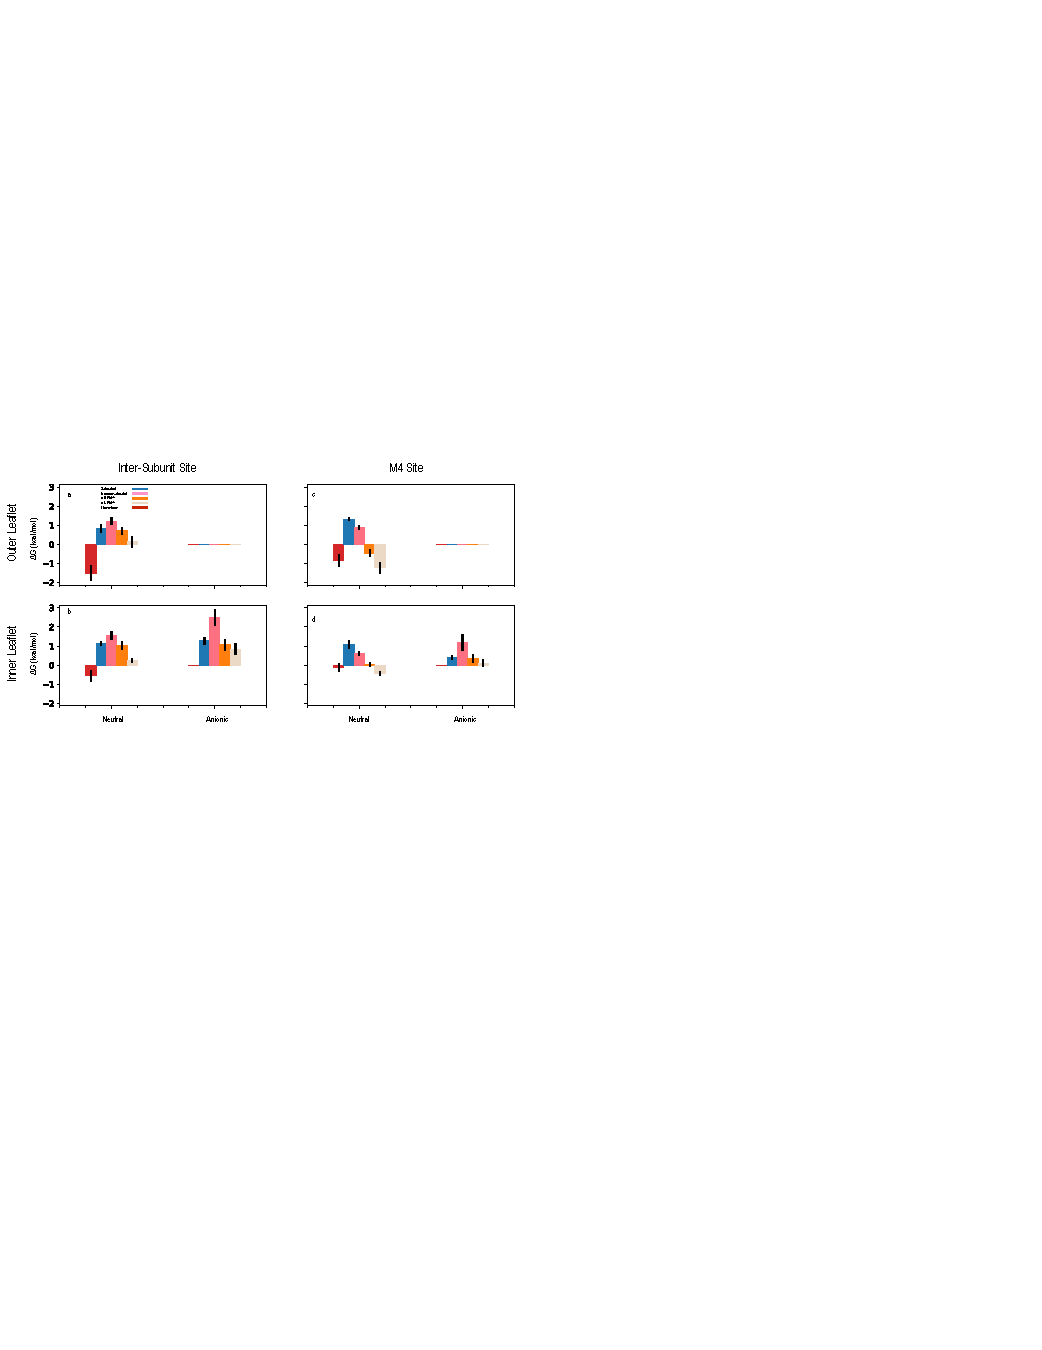
\includegraphics[width=\linewidth]{./Figures/Lipid_centric.pdf}
	\caption[\Newaffinities{} organized to reveal lipid preferences by site.] {Data shown is identical but reorganized and recolored from Figure \ref{fig:proBar}. Here, \newaffinities are colored by chain type (Saturated:blue, Monounsaturated:pink, n-6 PUFAs:orange, n-3 PUFAs:tan, Cholesterol:red), and separated by leaflet (rows) and site (columns).} %More negative values indicate stronger affinities, while more positive values indicate more displacement of the lipid by other lipid species. Data incorporates 10 replicas averaging over the last half of the 5$us$ trajectory, with five-fold averaging over each type of pseudosymmetric site. } {Affinity calculation ranking for neutral and anionic lipid saturation species averaged the final 2.5 $\mu s$ simulations for each 10 replicas by occupancy site. Occupancy sites are averaged from 5 sites.\grace{LMS:Isn't it five sites?} Row one is the outer leaflet and row two is the inner leaflet. Columns are charge, each subplot is a difference occupancy site.  Error bars are the standard error calculated over the 10 replicas simulated. The smaller the number the stronger the affinity. Colors: Saturated:blue, Monounsaturated:green, n-6 PUFAs:orange, n-3 PUFAs:red, Cholesterol:purple}
	\label{fig:lipidBar}
\end{figure*}

\subsection{Effect of Head Group Charge on Affinity Depends on Leaflet and Binding Site}
%Research by Tong et al 2019 \cite{Tong2019} showed anionic lipids favorably occupied around arginines in ELIC's inner inter-subunit site. We hypothesize \nachr's outer TMD and inner inter-subunit sites will have a strong affinity for neutral phospholipids and \nachr's inner M4 sites will have a strong affinity for anionic phospholipids because M4 has more cationic amino acids, see Figure \ref{fig:aaa}a. We test the proposed lipid distributions using both enrichment density analysis and affinity calculations.
Figure \ref{fig:acyl_map}b compares the density enrichment for anionic headgroups with that of neutral headgroups. Data is shown for the inner leaflet only, because anionic lipids are not present in the outer leaflet at the start of simulations and few anionic lipids flip flop to the outer leaflet.% Furthermore, as shown in Figure \ref{fig:lipidBar}C, the anionic lipids that do flip in to the outer leaflet (\grace{LMS: how many is this?}) \liam{I'm not sure. Versions of the manuscript have had comments trying to bring up anionic distributions and affinities with you previously. It looks like 1 - 5 lipids flip? }  have very weak affinity for any sites in the outer leaflet ($\geq 2.0$ kcal/mol). These results are consistent with our previous observations that POPG had very weak affinity for the outer leaflet sites of ELIC\cite{Tong2019}.

In the inner leaflet, the anionic lipids are expected to select for sites that are lined with basic amino acids, which are in different locations depending on subunit (Figure \ref{fig:aaa})  As shown in Figure \ref{fig:acyl_map}b, anionic lipids are generally enriched around the M3/M4 helices for the $\alpha_{\gamma}, \gamma,\delta,$ and $\beta$ subunits.  Anionic lipids are enriched at intersubunit sites and around M4 sites for all subunits but the $\alpha$ subunits. Non-$\alpha$ \nachr~ subunits have basic amino acids closer to M4 alpha-helices, as shown in Figure \ref{fig:aaa}.  We incorporate data from all five pseudo-symmetric sites to obtain the \newaffinities{} reported in Figure \ref{fig:proBar}B, which suggest that anionic lipids have significantly stronger affinities for M4 sites on average. The average anionic affinity difference between inter-subunit and M4 sites is $\sim -1.0$ kcal/mol, as shown in Figures \ref{fig:proBar}, \ref{fig:lipidBar}d and SI \ref{tab:avg_s}. Although the magnitude of the affinity difference varies with acyl chain saturation, the sign is unchanged.     %Neutral lipids have weak enrichment around M4 sites in the outer leaflet, but other wise are neutral.
%We hypothesize the difference in our result is from the number and placement of charged amino acids in ELIC's (TMD PDB:3RQW\cite{Pan2012}) versus that of neuromuscular \nachr. We use VMD \cite{HUMP96} to visualize the difference between \nachr~and ELIC's inner \notsure{leaflet} TMD, . Both pLGICs have a number of cationic amino acids around their annulus. ELIC has more cationic amino acids embedded in the protein density than at the annulus. \notsure{Cationic amino acids found in the \nachr~structure tend to be more outward facing than cationic amino acids in the ELIC structure.} Non-$\alpha$ \nachr~ subunits have cationic amino acids closer to M4 alpha-helices. ELIC has cationic amino acids closer to the inter-subunit sites. Anionic amino acids are found at \nachr M4 alpha-helices, with the exception of the $\beta$ subunit. Anionic amino acids are found closer to the M1/M4 alpha-helices interfaces in ELIC, or embedded within the \liam{inner/non-annular/bulk of} protein.
%At inter-subunit sites the same trend with acyl-chain persists: n-3 PUFAs $>$ n-6 PUFAs $>$ saturated $>$ monounsaturated.  %In the outer leaflet, \nachr~ has preferential binding with cholesterol, neutral PUFAs, and then monounsaturated or saturated, the later are dependent on site.  
We now switch again to the ``site perspective'' to compare whether inner leaflet sites would prefer occupancy by anionic or neutral lipids. % compare the affinity of anionic lipids for inter-subunit sites the lower leaflet, see Figure \ref{fig:lipidBar}b. 
As shown in Figure \ref{fig:lipidBar}C, lipid affinity values for inter-subunit sites are either insensitive to charge (saturated or n-6 PUFA chains) or weaker for anionic lipids by at least 0.5 kcal/mol (monounsaturated and n-3 PUFA chains).  In comparison, at the M4 site, saturated chains in anionic lipids have significantly stronger affinities than those in neutral lipids (a difference of $\sim$0.5 kcal/mol). All other lipid chains attached to anionic headgroups have weaker affinities for the M4 site. The clear trend observed in neutral lipids (stronger affinities for more flexible acyl chains) is thus broken in anionic lipids because saturated anionic lipids are so favorable.  %Anionic lipids in the inner leaflet have affinities $\sim 1.0$ kcal/mol stronger than in the outer leaflet, monounsaturated lipids are an exception.
% Anionic affinities are more favorable at inner inter-subunit sites than the outer leaflet, difference $\sim1.0$ kca/mol, excluding monounsaturated lipids. % have $\sim 1.0$ kcal/mol stronger affinity for the inter-subunit sites than in the outer leaflet.

%Next we compare the relative affinities for anionic lipids occupying M4 sites in the lower leaflet, see Figure \ref{fig:lipidBar}d. Unlike the inter-subunit sites,  anionic and neutral lipids have different affinity trends:  Anionic lipids continue to be non-monotonic: n-3 PUFAs $>$ n-6 PUFAs $>$ saturated $>$ monounsaturated, where neutral lipid affinities are related to the acyl-chain flexibility, the stronger the affinity the more flexible the acyl-chain. Anionic lipids are generally $<0.6$ kcal/mol, excluding monounsaturated lipids. Anionic lipids have stronger occupancy affinity values at M4 than at inter-subunit sites, regardless of saturation. 
%\subsubsection{Discussion}
In summary, we observe that binding sites have clear preferences for particular head group charge and acyl-chain saturation, suggesting \nachr~lipid occupancy to be driven in two steps, a ``coarse-sorting'' by head groups, and then ``fine-sorting'' by acyl-chains.  A neutral lipid will occupy \nachr's boundary region but acyl chains dictate where specific lipids occupy \nachr. Anionic lipids diverge from this pattern at the inner M4 site which has the strongest affinity for anionic lipids independent of saturation. 
%A potential mechanism for anionic lipid site occupation could be anionic lipids occupy M4 due to the number of positively charged amino acids until the site is saturated with anionic lipids, similar to Tong et al\cite{Tong2019}. The remainder anionic lipids do not all defuse back to the bulk membrane, they weakly interact with the inner inter-subunit site as a local anionic lipid pool for M4. 
\subsection{Role of Individual Lipid Headgroups in Determining Affinity}
%The NEW SECTION 3.3 : EFFECT OF HEADGROUP DETAILS ON LIPID AFFINITIES can instead be focused on the effect of specific headgroups
%Neutral lipids have a higher affinity in the outer leaflet. Neutral and anionic lipids show a level of competition at inner inter-subunit sites.  Anionic lipids have an acutely stronger affinity at inner M4 sites compared to neutral lipids. 
Neutral and anionic are bulk terms that categorize numerous lipid head-groups by charge. %Frequently head group charge and size play a factor in direct protein-lipid interactions. 
To understand the role of the chemical distinctions between head groups of like charge, we broke the headgroup affinities down by headgroup species in Table \ref{tab:dGOuterHG}.  %we introduce the anionic lipids with the strongest affinities for occupying \nachr~by leaflet and site.
%We measure head group affinities in the outer leaflet site, see Table \ref{tab:dGOuterHG}.  
In the outer leaflet, lipids contain a mixture of PE and PC headgroups. The small neutral PE head group has the strongest affinity across all headgroups for both inter-subunit and M4 sites, -0.2$\pm$0.3 and -1.1$\pm$0.2 kcal/mol respectively. The larger neutral PC headgroups are weaker than PE by $\sim > 0.5$ kcal/mol. In living cells, as in this neuronal membrane, PUFAs are more frequently tethered to PE than to PC or SM \cite{Isolated1969, Taguchi2010, Breckenridge1973,Ingolfsson2017b,Lorent2020}, so it is possible that this affinity simply reflects the high affinity of PUFA chains. However, even for identical chains, both experimental and simulation data \cite{Sharp2019} suggests stronger PE-ELIC than PC-ELIC interactions.  

Table \ref{tab:dGInnerHG} shows specific head group affinities in the inner leaflet. %Anionic lipids have a stronger  affinity in the inner leaflet compared to the outer leaflet, especially at the M4 sites. 
As in the outer leaflet, lipids with PE headgroups still have the strongest affinity of all lipids, but in the inner leaflet we are also able to distinguish affinities for anionic species. For the intersubunit site, PI, PS, and PC have similar affinities (within statistical error), and have significantly stronger affinities for these sites than the phosphoinositides (PIPS) PIP1, PIP2, PIP3, which have a significantly stronger affinity than phosphatidic acid  (PA). Thus, from strongest to weakest, PE$>$PI$\sim$PS$\sim$PC$>>$PIP1$\sim$PIP2$\sim$PIP3$>>$PA for the intersubunit site. In contrast, at the M4 site, more significant differences among moderate affinity headgroups emerge. PI has significantly stronger affinity than PS (a difference of 0.3$\pm$0.1 kcal/mol), and PS has a significantly stronger affinity than PC (a difference of 0.2$\pm$0.1 kcal/mol).% \grace{LMS please fill in the missing values. You may have them in some text I commented out, but I couldn't be sure. To get an overall error difference, remember that the error in X1 - X2 is $\sqrt{dx1^{2} + dx2^{2}}$ where dx1 and dx2 are the individual errors.} \liam{$\sqrt{dx1^{2} + dx2^{2}}$ is .14 for both PI vs PS and PS vs PC, rounded to .1}
From strongest to weakest, PE$>$PI$>$PS$>$PC$>>$PIP1\\$\sim$PIP2$\sim$PIP3$\sim$PA for the M4 site.    %PI and PS are $\sim 0.4 $ and $\sim 0.6$ kcal/mol weaker than PE (inter-subunit and M4 respectively), they are $\sim 0.1$ and $\sim0.4$kcal/mol stronger than PC at inter-subunit and M4 sites respectively. Other anionic lipids, phosphatidic acid  (PA) and phosphoinositides (PIPS) have affinity values $>2.2$ and $>1.8$ kcal/mol for inter-subunit and M4 sites respectively. 

%Sharp et al 2019\cite{Sharp2019} and Tong et al 2019\cite{Tong2019} observed slightly more enrichment of PE than PC around pLGICs. 

%\subsubsection{Discussion}

\begin{table}
	\caption[\Newaffinities () of neutral lipids for both sites in the outer leaflet, by head group.]{  Errors are standard errors (n=10 independent replicas). }
    \centering
    \begin{tabular}{|l||c|c|}
    \hline
	{} &   Intersubunit Sites&  M4 Sites\\
	{} & $\Delta$G (kcal/mol) & $\Delta$G (kcal/mol)\\
	\hline
	PE	&-0.2 $\pm$ 0.3& -1.1$\pm$0.2\\
	%PC	& 0.8 $\pm$0.3 &  0.5$\pm$0.2\\
	PC & 1.4$\pm$0.2&	1.1 $\pm$0.2\\
	%SM	&1.9$\pm$0.3 &  1.7$\pm$0.1\\
	\hline
    \end{tabular}
    \label{tab:dGOuterHG}
\end{table}

\begin{table}
	\caption[\Newaffinities ($\Delta$G) of neutral lipids for both sites in the inner leaflet, by head group.] {Values are sorted by strength of affinity for intersubunit sites. Errors are standard errors (n=10 independent replicas). }
    \centering
    \begin{tabular}{|l||c|c|}
    \hline
	{} &  Inner Inter Sites&  Inner M4 Sites\\
	{} & $\Delta$G (kcal/mol) & $\Delta$G (kcal/mol) \\
	\hline
	PE& 0.3$\pm$0.2& -0.1$\pm$0.1\\
	PI&0.9$\pm$0.3 &  0.2$\pm$0.1\\
	PS&1.0 $\pm$0.2	&  0.4$\pm$0.1\\
	%PC&1.2 $\pm$0.2	&  0.7$\pm$0.1\\\
	PC &1.0$\pm$0.2 &	0.9$\pm0.1$ \\
	%SM&2.2 $\pm$0.4	&  1.4 $\pm$0.1\\
	PIP3	&2.6$\pm$0.4	 &  1.8 $\pm$0.4\\
	PIP2	&2.8 $\pm$0.2	&  2.1$\pm$0.4\\
	PIP1	&2.4 $\pm$0.3	&  2.1$\pm$0.4\\
	PA	&3.0 $\pm$0.3	&  2.2$\pm$0.4\\
	\hline
    \end{tabular}
    \label{tab:dGInnerHG}
\end{table}

\section{Conclusions}

\label{con}

Using coarse-grained simulations of the \nachr{} within a quasi-neuronal membrane containing over thirty lipid species, we have observed spontaneous lipid binding and quantified lipid specificity for two types of sites in the protein TMD.  These two site classes represent the most concave (intersubunit site) and convex (M4 site) portions of the star-shaped \nachr~ and were initially observed as ``hot spots'' in our previous simulations\cite{Woods2019,Tong2019} of model membranes. Compared to classic ligand binding sites, these sites are superficial and have a large volume. The ``ligands'' occupying them are also non-traditional: lipids are flexible chain molecules that may only partially occupy the site and are likely to share the site with other partially-occupying ligands.  While our lab has developed promising alchemical approaches\cite{Salari2018} for calculating traditional affinities of atomistic lipids for more highly localized, well-defined sites, these hot spots required a different approach. Here we have proposed a softer ``\newaffinity'' for characterizing these affinities from spontaneous, unbiased coarse-grained simulations. While we restrict the use of this method here to \nachr, it should be straighforward to extend to any other transmembrane proteins with detectable regions of density enrichment. 

\begin{figure}
	\center
	%\includegraphics[width=\linewidth]{Summary.pdf}
	\includegraphics[width=3.5in]{./Figures/Summary.pdf}
	\caption[Cartoon of expected boundary lipids for the \nachr~ in a native membrane for both leaflets.] {Protein is shown in the center of both leaflets in a cyan floral shape. Grey and black outlines depict sites favorable for neutral and anionic lipids respectively. Fill color represents the lipids most likely to occupy each site (red: cholesterol, blue: saturated, beige: PUFA) and outline represents headgroup charge (gray: neutral, black: anionic).}
	\label{fig:sum}
\end{figure}

Our results are summarized graphically in Figure \ref{fig:sum}. Based on our results from model membranes, we had hypothesized that
%We used a neuronal lipid compositions modified from\cite{Ingolfsson2017b} to analyze \nachr~within a neuronal membrane. We defined lipid-protein occupancy from polar enrichemnt density plots and used Sharp\cite{Sharp2019}, Woods\cite{Woods2019}, and Tong\cite{Tong2019} to hypothesized lipid occupancy for each site. We hypothesized 
 PUFAs would select for the convex M4 sites and that raft-forming lipids like cholesterol and saturated lipids would select for the concave inter-subunit sites. Overall, our results were consistent with this expectation.  Yet although lipids containing PUFAs do prefer the M4 site to the intersubunit site, their affinity for even the intersubunit sites are stronger than that of all other phospholipids. This result underscores the reliable partitioning of \nachr{} to PUFA-rich, liquid-disordered domains that we observed in homoacidic, domain forming membranes\cite{Sharp2019}, and suggests PUFAs may have been absent from the intersubunit site in heteroacidic membranes\cite{Woods2019} because of the constraints of the lipid topology. In the latter simulations, all lipids contained one saturated chain and one PUFA chain, so binding of the PUFA chain to its preferred M4 site requires the saturated chain to find the most favorable location nearby (in the intersubunit site) and may block binding of other PUFA chains to that site.  These constraints are relaxed in the native neuronal membrane, which has a more diverse lipid composition with multiple different chain pairings; about 6\% of the phospholipids in our simulated membranes contain no saturated chain at all. Nonetheless, our previous results\cite{Woods2019} using simplified binary heteroacidic/cholesterol membranes played a key role in identifying the natural site boundaries.  

As expected, within each leaflet cholesterol has the strongest affinity for the inter-subunit sites, although the affinity of cholesterol for the M4 sites was second only to that of n-3 PUFAs. Combined, these results are consistent with an overwhelming amount of evidence spanning four decades that suggests direct interactions between cholesterol and \nachr s, regardless of the phospholipid composition of the membrane.  One surprise for cholesterol was the role of the leaflet in determining affinity: cholesterol has a stronger affinity for either outer leaflet site compared to either inner leaflet site. This result may reflect competition with anionic saturated lipids in the inner leaflet, which would be consistent with multiple experiments\cite{Baenziger2000,Wenz2005,Hamouda2006,Thompson2020}, suggesting that anionic lipids can partially or fully compensate for a loss of cholesterol.  This result is also consistent with cholesterol embedded\cite{Brannigan2008} in the outer TMD (which has numerous gaps in the amino acid density) but not the inner TMD. 
%Of the phospholipids analyzed, n-3 PUFAs have the strongest affinities across all sites, with affinities values of $\sim<0$ kcal/mol for M4 sites and $\sim<$.5 kcal/mol for inter-subunit sites. %We predict the relative high affinity for n-3 PUFAs are a result of their flexibility. The n-3 PUFA, DHA, has a number of unique membrane properties \cite{Stillwell2003a,Gawrisch2003}, and is observed to consistently interact with non-annular sites in and around \plgic s \cite{Sharp2019, Woods2019}. The inherent disorder in PUFAs and the strong affinity they have for M4 sites suggests PUFAs may minimize unfavorable membrane deformation\cite{Brannigan2006,Brannigan2007,Hu2012a,Argudo2016a,BuganzaTepole2017,Dan1993,Fournier2015} around \plgic's conical-star shape provided by M4.
%Similar to n-3 PUFAs cholesterol occupies sites nearly indiscriminately, though for each leaflet cholesterol has the strongest affinity at inter-subunit site. Cholesterol's affinity for the M4, compared to inter-subunit sites, is reduced by about $50\%$ and $80\%$ for the outer and inner leaflets respectively. However, unlike the phospholipids, cholesterol's affinity for each site is consistently $<0$ kcal/mol. %Brannigan et al 2008 \cite{Brannigan2008} hypothesized 15 non-annular cholesterol binding sites for \nachr. Sharp et al 2019 \cite{Sharp2019} observed cholesterol embedded in $\beta$ subunits of \nachr. It could be cholesterol's favorability for M4 is a result of its relative small size making it ideal for packing between alpha-helices.

%For most sites monounsaturated lipids have the weakest affinities ($>.5$ kcal/mol). We hypothesize this is due to packing limitation from monounsaturated lipids single acyl-chain kink. Cholesterol and PUFAs are small or highly flexible and readily fit at various sites in \plgic's topology. Saturated lipids, which lack any kinks and are more rigid than unsaturated lipids, may pack around inter-subunit site's ''flat'' topology. We argue the single acyl-chain kink found in monounsaturated lipids may prevent packing of itself around inter-subunit sites, and is not flexibility to compete with PUFA's occupying M4 sites. 

%Neutral lipids that occupy M4 have a unique trend in affinity. The affinity strength increase as a relation to acyl-chain flexibility, initially state in section \textit{Effect of Acyl-Chain on Neutral Lipid Affinities}. Neutral lipids at inter-subunit sites and all anionic lipids share a non-monotonic affinity trend where it is more akin to a concave function, see Figure \ref{fig:sum}. 

Based on our results using ELIC\cite{Tong2019}, we had expected that anionic lipids would select for sites on the inner leaflet lined with basic residues.  In the homomeric ELIC, these residues are symmetricly-arranged, while in the heteromeric \nachr{} they vary by subunit(Figure \ref{fig:aaa}a), with the M4 site containing the most such residues on most subunits. The present results support that expectation: %Yet unlike ELIC due to cationic amino acid distribution, see Figure \ref{fig:aaa}a. \nachr~ has cationic amino acids at both inter-subunit and M4 sites.
%Neutral lipids have a stronger affinity for the outer leaflet compared to anionic lipids. Neutral lipids found at the inner inter-subunit sites have slightly weaker affinities compared to the same lipids in the outer inter-subunit site. 
anionic lipids have a stronger affinity for M4 than inter-subunit sites.  %Inner anionic saturated, n-6 and n-3 PUFAs have significantly greater affinities than outer anionic lipids of the same saturation types. Monounsaturated lipids affinity values do not change much between leaflets ($\sim 0.5$ kcal/mol). We associate anionic lipids have stronger affinity for M4 in \nachr~compared to ELIC due to cationic amino acid distribution, see Figure \ref{fig:aaa}a. \nachr~ has cationic amino acids at both inter-subunit and M4 sites.

For both outer and inner leaflets, neutral lipids with smaller head groups (PE) have stronger affinity than the larger PC headgroup. It is unclear why PE is more favorable than other neutral lipids at this time, though this is consistent with previous work \cite{Sharp2019,Tong2019}, and the most straightforward explanation is that the smaller headgroup introduces fewer clashes with the protein TMD. % It may be due to the frequency which PE are attached to lipids with PUFAs or the size of the head group.  However, many of the the anionic lipid head groups are attached to PUFAs.

Among anionic lipids in the inner leaflet, regardless of the site, PS and PI have an affinity greater than or equal to PC, and much greater than the other anionic lipid headgroups (PIP1,PIP2,PIP3, and PA).   The lipid headgroups PS and PI both have a charge of -1, while PA in the MARTINI forcefield\cite{DeJong2012} carries a charge of -2, and PIP1, PIP2, and PIP3 have charges of -3,-5, and -7. These results suggest that the inner leaflet sites select for monoanionic headgroups, while multianionic headgroups are highly unfavorable.  Due to the limitations of the coarse-grained model, future atomistic calculations are required to validate and understand the apparent preference of the M4 site for PI over PS.  %These differences cannot be attributed to size alone: the bulkier PI (four martini beads) and the small PS (two martini beads) have comparable affinities which are both much greater than both the bulky PIPS and the smallest headgroup, PA. 

The present results highlight the utility of model membranes for developing hypotheses of specific lipid-protein interactions, and the need to test those hypothesis within more complex native membranes. The present results could be tested and aid in interpretation of experiments carried out in more complex membranes. For instance, we would expect that mutations of the basic residues facing the inner leaflet would reduce binding of saturated phospholipids with anionic headgroups, which would be replaced with bound cholesterol. We would also predict that if PUFAs cause gain of function via binding to the intersubunit site, this gain would be enhanced by replacing some heteroacidic lipids with homoacidic lipids while keeping the total fraction of PUFA chains constant. In general the present results provide valuable insight into how to predict lipid competition, which is one of the primarily challenges of interpreting experiments in complex membranes.  
%.  PA has the weakest affinity of the anionic lipids, though it has the smallest head group (only a phosphate), and PIPS which are much bulkier than all the other head groups are comparable to PA. PI, PS  share the same charge: -1.0 C. 


%Why one head group interacts more favorably is still unknown. It may be a product of head group to acyl-chain combination, evolution, or the coarse grained model. The PE head group bead types are Qd and Qa, which are attracted to most of the other bead types. PS has P5 and a QA, where P5 is attractive to about half the bead types and repulsive to the other half. PI has coarse-grained ring of P5 and P1s, and Qa, all of which tend to be attractive to other beads.  



%It is unclear why neutral and anionic head group affinities are uncorrelated, though it may be a product of head group to acyl-chain combination, evolution, or the coarse grained model. \notsure{The PE head group bead types are Qd and Qa, which are attracted to most of the other bead types. PS has P5 which is attractive to about half the bead types and repulsive to the other half. PI has coarse-grained ring of P5 and P1s, and Qa, all of which tend to be attractive to other beads. }

%\nachr~lipid occupancy appears to be driven in two steps. First a ''coarse-sorting'' by head groups, and second ''fine-sorting'' by acyl-chains. In the outer leaflet anionic lipids are clearly unfavorable, coarse-sorting. A neutral lipid will occupy \nachr's boundary region and then there is ''fine-sorting'' by acyl-chain saturation. Inner Inter subunit sites have competition between lipid head group charge, but have specific acyl-chain affinity. The inner M4 site has the strongest affinity for anionic lipids regardless of saturation type, which diverges from the proposed occupancy driver. 
%
%Inner anionic lipid occupancy could be driven by another mechanism: anionic lipids occupy M4 due to the number of positively charged amino acids until the site is saturated with anionic lipids, similar to Tong et al\cite{Tong2019}. The remainder anionic lipids do not defusing back to the bulk membrane, they weakly interact with the inner inter-subunit site as a local anionic lipid pool for M4. 

% Raft forming lipids have higher affinities for inter-subunit sites over M4, but cholesterol has unexpectedly strong affinity for all sites. Unsaturated lipids have a highest affinity for M4, however, n-3 PUFAs show strong affinity for inter-subunit sites as well  with a difference of about 1 kcal/mol. These results suggest when neutral lipids are available for \nachr's boundary membrane, degree of saturation and molecule size play vital roles. Saturated and monounsaturated lipids, which tend to maintain a higher degree of order when compared to  PUFAs, show poor affinity in-comparison to more flexible lipids. While, saturated and monounsaturated lipids show relative high and low affinity sites within their saturation species, highly flexible PUFAs and small cholesterol occupy \nachr's density gaps more readily.


\section*{Acknowledgments}
GB and LS were supported by the Busch Biomedical Foundation. This project was supported by generous allocation through the Rutgers University Office of Advanced Research Computing (OARC), which is supported by Rutgers University and the state of New Jersey. We are grateful to Dr. J{\'{e}}r{\^{o}}me H{\'{e}}nin for helpful input and suggestions.

\section*{Data Availability Statement}
The data that support the findings of this study are available from the corresponding author upon reasonable request. Scripts for polar density analysis and plotting scripts can be found on github: https://github.com/BranniganLab/densitymap. 
%Using $\Delta G$ free energy to calculate the occupancy affinities, we find n-3 PUFAs and cholesterol \textit{nearly} indiscriminately occupy any region of the protein, cholesterol favors inter-subunit sites and n-3 PUFAs favor M4 sites. Anionic lipids are unfavorable in the outer leaflet. Anionic lipids and neutral lipids occupy at comparable affinities in the inner inter-subunit sites, see Figure \ref{fig:sum}.

%These results show a significant divergence from our proposed hypothesis and are depicted in figure \ref{fig:sum}. In the outer leaflet neutral have a strong affinity to occupy sites. Unsaturated lipids and cholesterol occupy the M4 site, while n-3 PUFAs, cholesterol, and saturated lipids occupy inter-subunit sites. Neutral and anionic lipids occupy inner inter-subunit sites with similar lipid composition compared to the outer leaflet. Inner M4 sites have a strong affinity for anionic lipids regardless of acyl chain.

%% The Appendices part is started with the command \appendix;
%% appendix sections are then done as normal sections
%% \appendix

%% \section{}
%% \label{}

%% References
%%
%% Following citation commands can be used in the body text:
%% Usage of \cite is as follows:
%%   \cite{key}          ==>>  [#]
%%   \cite[chap. 2]{key} ==>>  [#, chap. 2]
%%   \citet{key}         ==>>  Author [#]

%% References with bibTeX database:

%\bibliographystyle{model1-num-names}
%\bibliography{Paper_Bibs}

%% Authors are advised to submit their bibtex database files. They are
%% requested to list a bibtex style file in the manuscript if they do
%% not want to use model1-num-names.bst.

%% References without bibTeX database:

% \begin{thebibliography}{00}

%% \bibitem must have the following form:
%%   \bibitem{key}...
%%

% \bibitem{}

% \end{thebibliography}
%\begin{table}
%    \caption{Lipid ratios used for neuronal simulations grouped by head group.}
%    \label{tab:rats}
%    \centering
%
%\begin{tabular}{|c||c|cc|}
%
%\hline
%Head Group & Lipids & Outer (\%) &{Inner (\%)} \\ \hline\hline
%{}&CHOL                         & 44.3     & 40.67                         \\
%\hline
%PC &{} &30.5&15\\ \hline
%{} &DPPC                         & 6.7      & 3.3                           \\
%{} &DOPC                         & 2.8      & 1.4                           \\
%{} &POPC                         & 11     & 5.4                         \\
%{} &PFPC                         & 0.7      & 0.4                           \\
%{} &PAPC                         & 5.9      & 2.9                           \\
%{} &PUPC                         & 2.1      & 1.0                           \\
%{} &OIPC                         & 0.7      & 0.4                           \\
%{} &OUPC                         & 0.5      & 0.3                           \\
%\hline
%\hline
%PE &{} &13.8&23.4\\ \hline
%{} &POPE                         & 1.6      & 2.7                           \\
%{} &PAPE                         & 4      & 6.7                           \\
%{} &PUPE                         & 6.3      & 10.7                          \\
%{} &OIPE                         & 0.2      & 0.3                           \\
%{} &OAPE                         & 0.9      & 1.5                           \\
%{} &OUPE                         & 0.9      & 1.5                          \\
%\hline
%\hline
%SM &{} &11.3&2.5\\ \hline
%{} &DPSM                         & 7.4      & 1.7                           \\
%{} &PBSM                         & 1.4      & 0.3                           \\
%{} &POSM                         & 0.9      & 0.2                           \\
%{} &PNSM                         & 1.7     & 0.4                           \\
%\hline
%\hline
%PS &{} &0.0&10.8\\ \hline
%{} &DPPS                         & 0.0      & 0.5                           \\
%{} &POPS                         & 0.0      & 2.7                           \\
%{} &PAPS                         & 0.0      & 3.0                           \\
%{} &PUPS                         & 0.0      & 3.8   			\\      
%{} &OUPS                         & 0.0      & 0.8                           \\
%\hline       
%\hline          
%PA &{} &0.0&0.4\\ \hline
%{} &POPA                         & 0.0      & 0.1                          \\
%{} &PAPA                         & 0.0      & 0.3                           \\
%\hline
%\hline
%PI &{} &0.0&2.3\\ \hline
%{} &POPI                         & 0.0      & 1.4                         \\
%{} &PIPI                         & 0.0      & 0.6                           \\
%{} &PAPI                         & 0.0      & 1.4                           \\
%{} &PUPI                         & 0.0      & 2.3                           \\
%\hline
%\hline
%PIPS &{} &0.0&1.5\\ \hline
%{} &POP1                         & 0.0      & 0.2                           \\
%{} &PAP1                         & 0.0      & 0.3                           \\
%{} &POP2                         & 0.0      & 0.2                           \\
%{} &PAP2                         & 0.0      & 0.3                           \\
%{} &POP3                         & 0.0      & 0.2                           \\
%{} &PAP3                         & 0.0      & 0.3                           \\
%\hline
%\end{tabular}
%\end{table}
%
%\begin{figure*}[!h]
%	\center
%	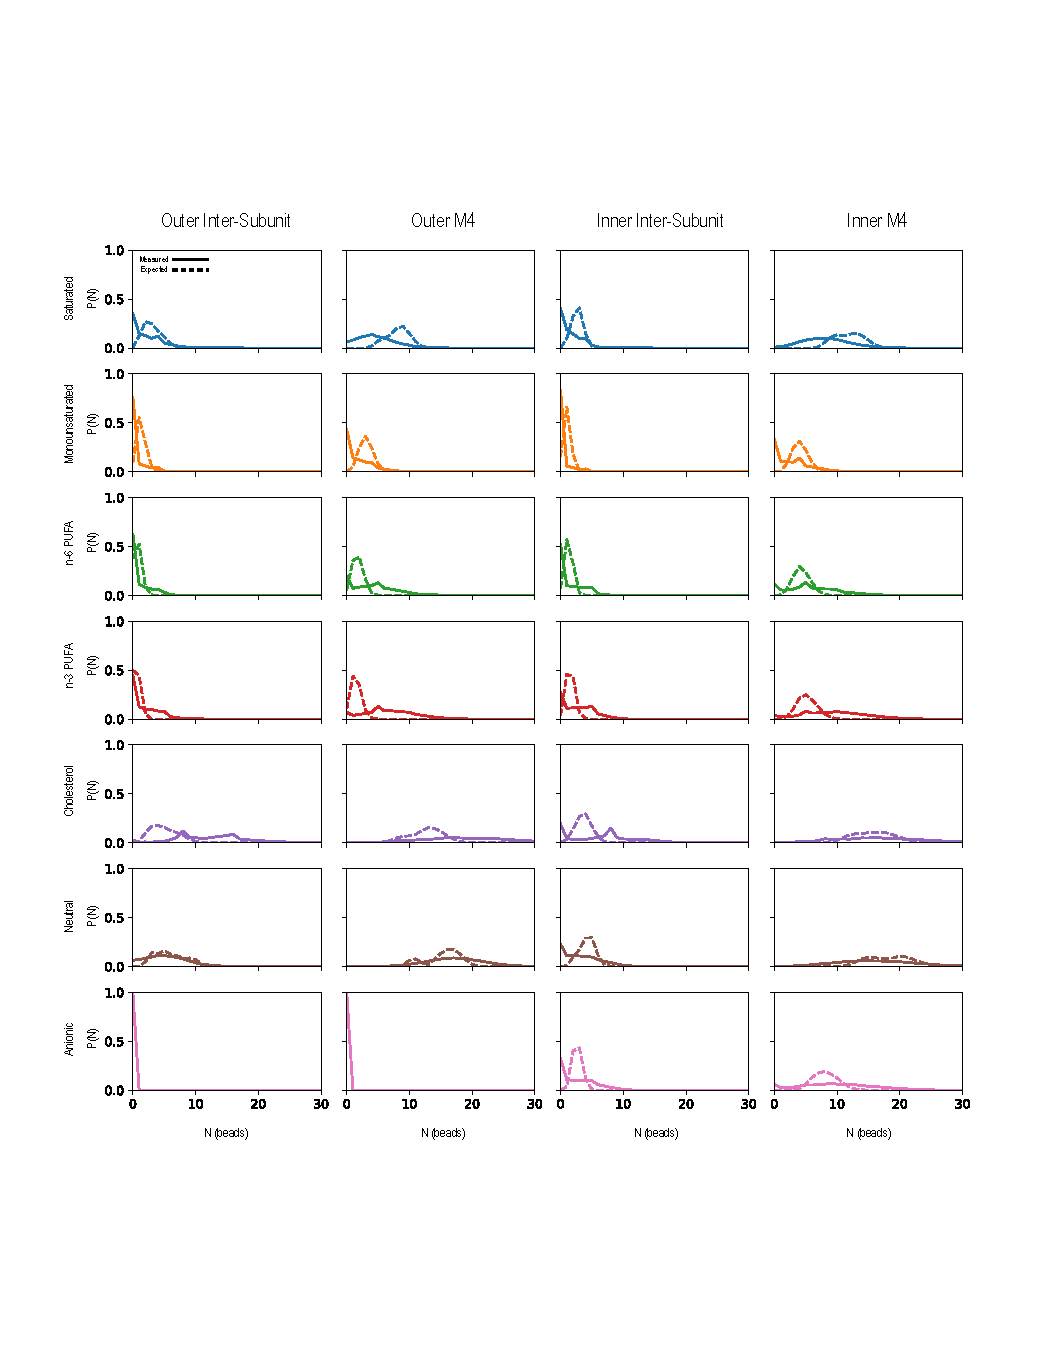
\includegraphics[width=\linewidth]{Bead_Distributions.pdf}
%	\caption{SI:Probability distributions of acyl-chain saturations, including cholesterol, and head group charge. Solid lines are probability of a given number of beads found at occupancy site, averaged over both the course of the simulation and subunit sites. Dashed lines represent the probability of a given number of beads in the bulk averaged over time. Bulk areas are square areas of equal area of occupancy sites.}
%	\label{fig:lipidDist}
%\end{figure*}
%
%\begin{table*}
%    \caption{Affinity values averaged over 10 replicas. $\Delta G$ values for averaged occupancy sites.}
%    \centering
%  \resizebox{\textwidth}{!}{  \begin{tabular}{|l||cc|cc|}
%        
%        \hline
%        {} &  Outer Inter Sites&  Outer M4 Sites&  Inner Inter Sites&  Inner M4 Sites\\
%        {} & kcal/mol & kcal/mol & kcal/mol & kcal/mol \\
%        \hline
%        
%        CHOL &-1.5 $\pm$0.4& -0.8$\pm$0.3&    -0.6$\pm$0.3& -0.1$\pm$0.2\\
%        Sat   &  0.7 $\pm$0.3	&  1.3 $\pm$0.2&     1.0 $\pm$	0.2&  1.1 $\pm$0.2 \\
%        Mono   &    1.2 $\pm$0.2&  0.8$\pm$	0.2&     1.4 $\pm$0.1&  0.7 $\pm$0.2\\
%        n-6   &         0.6 $\pm$0.2& -0.5 $\pm$0.1&0.3 $\pm$0.2& -0.3 $\pm$0.2\\
%        n-3   &       -0.0 $\pm$0.4& -1.3 $\pm$0.3&    -0.2$0.2\pm$ & -0.9$\pm$0.2\\
%        \hline
%        Neutral &     0.4 $\pm$0.3& -0.4$\pm$0.2 &     0.5 $\pm$0.2&  0.5$\pm$0.2 \\
%        Anionic &     2.4 $\pm$0.4&  2.4 $\pm$0.4&     0.3 $\pm$0.2& -0.3 $\pm$0.1\\
%	\hline
%        \hline
%        Sat Neutral &  0.8 $\pm$0.2&  1.3 $\pm$0.1&     1.1$\pm$0.1 &  1.1 $\pm$0.2\\
%        Mono Neutral & 1.2$\pm$0.2&  0.9 $\pm$0.1&     1.6 $\pm$0.2&  0.6 $\pm$0.1\\
%        n-6 Neutral &  0.7 $\pm$0.2& -0.5 $\pm$0.2&     1.0 $\pm$0.2&  0.0 $\pm$0.1\\
%        n-3 Neutral &  0.1 $\pm$0.3& -1.2$\pm$0.3& 0.2 $\pm$0.1& -0.4 $\pm$0.1\\
%        \hline
%        \hline
%        Sat Anionic & 2.5 $\pm$0.4&2.4$\pm$0.4& 1.3$\pm$0.2 &  0.4$\pm$0.1\\
%        Mono Anionic &3.0$\pm$0.5&2.7 $\pm$0.5& 2.5 $\pm$0.4&  1.2 $\pm$0.4\\
%        n-6 Anionic &2.9 $\pm$0.5	&2.7 $\pm$0.5&1.1 $\pm$0.3&  0.3$\pm$0.2\\
%        n-3 Anionic &2.8 $\pm$0.5	& 2.6 $\pm$0.5	& 0.8 $\pm$0.3&  0.1 $\pm$0.2\\
%        \hline
%
%        \hline
%        
%    \end{tabular}}
%    \label{tab:dGTab}
%\end{table*}
%
%\begin{table}
%    \caption{Affinity values averaged over 10 replicas. $\Delta G$ values for each occupancy sites.}
%    \centering
%\resizebox{\textwidth}{!}{\begin{tabular}{| c || cccccccccccccccccccc |}
%\hline
%   Lipids     & Outer $\alpha_{\gamma}-\beta$  & Outer $\beta-\delta$ & Outer $\delta-\alpha_{\delta}$  & Outer $\alpha_{\delta}-\gamma$  & Outer \gamma-\alpha_{\gamma}$  & Outer $\alpha_{\gamma}$   & Outer $\beta$   & Outer $\delta$    & Outer $\alpha_{\delta}$   & Outer $\gamma$   & Inner $\alpha_{\gamma}-\beta$  & Inner $\beta-\delta$  & Inne$\delta-\alpha_{\delta}$ & Inner $\alpha_{\delta}-\gamma$  & Inner $\gamma-\alpha_{\gamma}$  & Inner $\alpha_{\gamma}$    & Inner$\beta$   & Inner $\delta$    & Inner $\alpha_{\delta}$    & Inner $\gamma$   \\
%        \hline
%        & (kcal/mol) & (kcal/mol) & (kcal/mol) & (kcal/mol) & (kcal/mol) & (kcal/mol) & (kcal/mol) & (kcal/mol) & (kcal/mol) & (kcal/mol) & (kcal/mol) & (kcal/mol) & (kcal/mol) & (kcal/mol) & (kcal/mol) & (kcal/mol) & (kcal/mol) & (kcal/mol) & (kcal/mol) & (kcal/mol) \\ \hline \hline
%Lipid Species &&&&&&&&&&&&&&&&&&&&\\\hline
%CHOL    & -0.9       & -1.4       & -1.5       & -1.6       & -2.0       & -1.0       & -1.3       & -0.8       & -0.8       & -0.2       & -0.4       & -0.4       & -1.1       & 0.3        & -1.2       & -0.3       & 0.2        & -0.4       & -0.3       & 0.3        \\
%DOPC    & 3.5        & 3.4        & 2.2        & 2.8        & 2.3        & 1.8        & 2.1        & 1.5        & 1.5        & 1.9        & 2.4        & 3.1        & 2.9        & 2.6        & 2.9        & 1.6        & 1.4        & 1.8        & 1.5        & 1.6        \\
%DPPC    & 3.3        & 2.1        & 2.3        & 1.4        & 2.0        & 1.3        & 2.0        & 1.7        & 2.2        & 1.8        & 1.9        & 2.7        & 2.1        & 2.3        & 2.1        & 1.1        & 1.1        & 1.4        & 1.2        & 1.3        \\
%DPPS    & 4.1        & 4.1        & 4.2        & 3.9        & 4.2        & 3.5        & 3.8        & 3.7        & 3.7        & 3.6        & 4.4        & 4.2        & 3.5        & 4.9        & 5.3        & 2.2        & 2.6        & 2.9        & 2.6        & 3.1        \\
%DPSM    & 2.1        & 2.7        & 2.3        & 1.2        & 2.1        & 1.6        & 1.5        & 1.7        & 1.7        & 2.0        & 2.5        & 1.7        & 2.1        & 2.6        & 2.5        & 1.6        & 1.3        & 1.6        & 1.3        & 1.6        \\
%OAPE    & 1.9        & 2.5        & 1.9        & 1.4        & 1.9        & 1.5        & 1.3        & 1.3        & 0.9        & 1.1        & 2.3        & 2.5        & 1.9        & 1.9        & 3.1        & 1.4        & 1.3        & 1.5        & 1.2        & 1.4        \\
%OIPC    & 3.0        & 2.9        & 2.4        & 4.0        & 2.6        & 2.2        & 1.8        & 2.8        & 2.1        & 2.2        & 3.1        & 2.9        & 3.8        & 3.0        & 3.4        & 2.1        & 2.0        & 2.2        & 2.0        & 1.9        \\
%OIPE    & 2.4        & 4.0        & 3.5        & 3.8        & 2.4        & 2.0        & 2.2        & 3.1        & 2.6        & 2.8        & 4.9        & 3.3        & 3.5        & 3.8        & 3.3        & 2.2        & 2.8        & 2.7        & 2.1        & 2.4        \\
%OUPC    & 2.0        & 2.2        & 1.9        & 1.7        & 2.9        & 1.7        & 1.5        & 1.5        & 1.5        & 1.3        & 3.1        & 3.2        & 2.3        & 2.7        & 2.1        & 2.2        & 2.3        & 2.6        & 2.0        & 1.6        \\
%OUPE    & 0.9        & 1.0        & 1.4        & 2.0        & 1.7        & 0.6        & 0.8        & 0.8        & 0.9        & 0.9        & 2.4        & 1.4        & 1.5        & 1.8        & 1.7        & 1.2        & 1.0        & 1.0        & 0.9        & 0.8        \\
%OUPS    & 3.7        & 3.8        & 3.5        & 3.7        & 3.4        & 3.2        & 3.3        & 3.6        & 3.3        & 3.4        & 2.4        & 2.8        & 1.5        & 2.2        & 2.1        & 1.5        & 2.0        & 1.6        & 1.5        & 1.6        \\
%PAP1    & 4.6        & 4.2        & 4.3        & 4.4        & 4.4        & 4.0        & 4.3        & 3.9        & 4.3        & 4.0        & 1.4        & 3.3        & 1.5        & 1.6        & 2.9        & 2.6        & 1.7        & 2.4        & 1.9        & 1.3        \\
%PAP2    & 4.9        & 4.6        & 4.9        & 5.3        & 3.9        & 4.2        & 4.4        & 4.6        & 4.6        & 3.9        & 1.9        & 3.9        &            & 1.1        & 2.1        & 2.7        & 1.7        & 2.8        & 2.4        & 1.1        \\
%PAP3    & 4.2        & 4.1        & 4.2        & 4.0        & 4.3        & 3.9        & 4.1        & 3.9        & 3.6        & 3.9        & 2.7        & 1.7        & 3.2        & 1.6        & 2.0        & 2.0        & 1.9        & 1.3        & 2.3        & 1.1        \\
%PAPA    & 4.9        & 4.0        & 4.2        & 4.3        & 4.4        & 4.4        & 4.4        & 3.9        & 3.9        & 4.4        & 3.9        & 2.4        & 2.7        & 3.1        & 3.2        & 2.6        & 1.9        & 2.4        & 2.6        & 2.0        \\
%PAPC    & 0.6        & 0.9        & 1.0        & 1.1        & 1.2        & 0.2        & 0.3        & 0.5        & 0.3        & 0.2        & 1.7        & 1.7        & 1.7        & 1.6        & 1.9        & 0.8        & 0.8        & 0.9        & 0.7        & 0.8        \\
%PAPE    & 1.1        & 1.2        & 1.1        & 1.4        & 1.2        & 0.4        & 0.3        & 0.1        & 0.4        & 0.4        & 0.9        & 1.5        & 1.1        & 1.4        & 1.2        & 0.4        & 0.4        & 0.5        & 0.3        & 0.4        \\
%PAPI    & 3.2        & 3.3        & 3.6        & 3.3        & 3.3        & 3.0        & 3.0        & 3.4        & 3.1        & 3.1        & 1.7        & 1.7        & 1.9        & 1.6        & 1.4        & 1.2        & 1.1        & 1.0        & 1.2        & 1.1        \\
%PAPS    & 3.1        & 3.0        & 3.0        & 3.0        & 3.1        & 2.9        & 3.0        & 2.8        & 2.8        & 2.9        & 1.5        & 2.2        & 1.8        & 1.7        & 1.7        & 0.8        & 0.9        & 1.1        & 1.0        & 0.7        \\
%PBSM    & 4.9        & 4.9        & 3.4        & 4.4        & 3.1        & 2.7        & 3.0        & 3.5        & 2.7        & 2.9        & 3.2        & 3.5        & 3.5        & 3.8        & 3.5        & 2.2        & 2.1        & 2.3        & 2.5        & 2.5        \\
%PFPC    & 1.9        & 1.3        & 2.4        & 3.1        & 3.3        & 2.0        & 1.3        & 1.9        & 1.8        & 1.7        & 2.2        & 2.6        & 2.9        & 2.6        & 3.6        & 2.2        & 2.0        & 2.1        & 1.9        & 2.1        \\
%PIPI    & 4.0        & 4.6        & 3.9        & 4.6        & 4.2        & 3.5        & 3.7        & 3.5        & 3.7        & 4.4        & 3.6        & 2.9        & 1.8        & 3.3        & 2.4        & 2.3        & 2.1        & 2.3        & 1.8        & 2.7        \\
%PNSM    & 3.2        & 4.9        & 2.5        & 4.3        & 2.7        & 2.3        & 2.3        & 2.5        & 2.5        & 2.6        & 3.0        & 2.8        & 2.8        & 3.6        & 3.2        & 2.4        & 2.1        & 2.1        & 1.9        & 2.5        \\
%POP1    & 4.3        & 4.6        & 5.3        & 4.3        & 4.4        & 4.3        & 4.0        & 4.9        & 5.3        & 4.1        & 5.3        &            & 3.2        & 3.3        & 4.6        & 3.6        & 3.5        & 2.9        & 3.0        & 2.6        \\
%POP2    & 4.6        & 5.3        &            & 4.9        &            & 4.9        & 4.9        & 5.3        & 5.3        & 4.2        & 3.5        & 3.5        & 3.5        & 3.4        &            & 3.9        & 2.6        & 2.4        & 3.0        & 2.6        \\
%POP3    & 4.3        & 4.6        & 5.3        &            & 4.9        & 4.2        & 4.3        & 4.6        & 4.6        & 4.9        & 3.2        & 4.4        &            & 3.4        &            & 2.9        & 2.9        & 2.9        & 3.3        & 2.2        \\
%POPA    &            & 5.3        &            &            &            & 5.3        & 4.9        & 4.9        & 4.9        & 5.3        &            &            & 5.3        & 5.3        &            & 3.1        & 3.2        & 3.8        & 3.1        & 3.4        \\
%POPC    & 2.2        & 1.8        & 1.7        & 2.0        & 1.6        & 1.1        & 1.4        & 1.5        & 1.4        & 1.7        & 2.4        & 1.7        & 2.0        & 2.0        & 1.8        & 0.9        & 1.0        & 0.9        & 0.9        & 1.1        \\
%POPE    & 2.8        & 2.6        & 2.4        & 3.0        & 2.6        & 1.9        & 1.9        & 1.7        & 1.7        & 2.3        & 2.7        & 3.0        & 2.6        & 3.4        & 2.4        & 1.3        & 1.3        & 1.6        & 1.4        & 1.6        \\
%POPI    & 3.6        & 3.4        & 3.6        & 3.6        & 3.5        & 3.3        & 3.3        & 3.1        & 3.3        & 3.1        & 2.4        & 2.9        & 2.5        & 2.4        & 2.3        & 1.5        & 1.6        & 1.7        & 1.3        & 1.7        \\
%POPS    & 3.3        & 3.2        & 3.1        & 3.1        & 3.0        & 2.8        & 3.0        & 2.9        & 2.8        & 2.7        & 2.7        & 3.0        & 1.7        & 3.8        & 2.8        & 1.6        & 1.6        & 1.5        & 1.5        & 1.8        \\
%POSM    & 3.3        & 2.6        & 3.8        & 2.9        & 3.4        & 2.7        & 2.8        & 2.8        & 2.9        & 2.9        & 3.9        & 4.1        & 2.7        & 4.3        & 3.4        & 2.5        & 2.7        & 2.9        & 2.8        & 2.6        \\
%PUPC    & 1.4        & 1.5        & 1.9        & 1.0        & 1.9        & 0.5        & 0.8        & 1.0        & 0.8        & 0.5        & 2.0        & 1.7        & 1.7        & 2.1        & 2.0        & 1.5        & 1.2        & 1.5        & 1.1        & 1.0        \\
%PUPE    & -0.0       & 0.3        & 0.1        & -0.5       & 0.2        & -0.3       & -0.6       & -0.6       & -1.0       & -0.9       & 0.1        & 0.2        & 0.4        & 0.5        & 0.4        & -0.1       & -0.4       & -0.1       & -0.1       & -0.3       \\
%PUPI    & 3.2        & 3.2        & 3.0        & 3.1        & 3.1        & 2.8        & 3.0        & 2.9        & 2.9        & 2.8        & 1.0        & 1.0        & 1.4        & 1.1        & 0.7        & 0.9        & 0.4        & 0.4        & 0.9        & 0.3        \\
%PUPS    & 2.8        & 2.8        & 2.8        & 2.9        & 2.8        & 2.6        & 2.7        & 2.6        & 2.7        & 2.7        & 1.2        & 1.7        & 1.0        & 1.5        & 1.6        & 0.9        & 0.7        & 0.5        & 0.8        & 0.7        \\
%\hline
%\hline
%Head Groups &&&&&&&&&&&&&&&&&&&&\\\hline
%PC      & 0.9        & 0.4        & 1.0        & 0.7        & 1.1        & 0.3        & 0.2        & 0.8        & 0.8        & 0.3        & 1.1        & 1.0        & 1.1        & 1.2        & 1.5        & 0.6        & 0.7        & 0.8        & 0.7        & 0.6        \\
%PE      & -0.4       & -0.3       & -0.2       & -0.3       & 0.4        & -0.7       & -1.0       & -1.3       & -1.3       & -1.2       & -0.1       & 0.3        & 0.3        & 0.4        & 0.6        & -0.0       & -0.2       & -0.3       & -0.1       & -0.1       \\
%SM      & 1.9        & 2.5        & 2.2        & 1.2        & 2.0        & 1.5        & 1.6        & 1.8        & 1.8        & 1.9        & 2.4        & 1.7        & 1.9        & 2.6        & 2.5        & 1.4        & 1.4        & 1.4        & 1.1        & 1.6        \\
%PS      & 2.5        & 2.6        & 2.5        & 2.6        & 2.5        & 2.4        & 2.5        & 2.4        & 2.4        & 2.4        & 0.8        & 1.4        & 0.5        & 1.1        & 1.4        & 0.3        & 0.5        & 0.3        & 0.5        & 0.3        \\
%PA      & 4.9        & 3.9        & 4.2        & 4.3        & 4.4        & 4.3        & 4.2        & 3.8        & 3.8        & 4.3        & 3.7        & 2.5        & 2.6        & 3.1        & 3.3        & 2.5        & 1.8        & 2.4        & 2.5        & 2.0        \\
%PI      & 2.7        & 2.8        & 2.8        & 2.9        & 2.7        & 2.5        & 2.6        & 2.6        & 2.6        & 2.6        & 0.9        & 0.9        & 1.0        & 0.9        & 1.0        & 0.4        & 0.2        & 0.1        & 0.4        & 0.1        \\
%PIP1     & 4.3        & 4.1        & 4.2        & 4.0        & 4.2        & 3.8        & 3.9        & 3.9        & 4.6        & 3.7        & 1.5        & 3.6        & 1.6        & 2.0        & 3.3        & 2.7        & 1.8        & 2.3        & 2.1        & 1.4        \\
%PIP2     & 4.3        & 4.4        & 5.3        & 4.9        & 3.9        & 4.4        & 4.3        & 4.9        & 4.9        & 3.9        & 2.1        & 4.0        & 4.1        & 1.3        & 2.4        & 2.8        & 1.7        & 2.3        & 2.4        & 1.2        \\
%PIP3     & 4.0        & 4.0        & 4.2        & 4.2        & 4.2        & 3.9        & 3.9        & 3.9        & 3.6        & 3.8        & 3.3        & 2.2        & 3.6        & 1.8        & 2.3        & 2.0        & 2.1        & 1.4        & 2.3        & 1.2        \\ 
%\hline
%\hline
%Acyl-Chain Saturation &&&&&&&&&&&&&&&&&&&&\\\hline
%Sat      & 1.0        & 0.6        & 0.9        & 0.5        & 0.7        & 1.0        & 1.0        & 1.3        & 1.9        & 1.4        & 0.7        & 1.1        & 0.9        & 1.1        & 1.3        & 0.9        & 1.2        & 0.8        & 1.4        & 1.2        \\
%Monounsat      & 1.1        & 1.1        & 1.1        & 1.3        & 1.4        & 0.8        & 0.7        & 0.7        & 0.7        & 1.1        & 1.4        & 1.5        & 0.9        & 1.4        & 1.6        & 0.4        & 0.8        & 0.5        & 0.8        & 0.9        \\
%n-6      & 0.4        & 0.5        & 0.8        & 0.7        & 0.7        & -0.4       & -0.6       & -0.3       & -0.5       & -0.4       & 0.1        & 0.6        & 0.3        & -0.0       & 0.7        & -0.1       & -0.4       & -0.3       & -0.1       & -0.6       \\
%n-3      & -0.2       & -0.2       & -0.0       & -0.1       & 0.5        & -1.1       & -1.2       & -1.0       & -1.3       & -1.8       & -0.3       & -0.0       & -0.3       & -0.2       & 0.1        & -0.5       & -1.0       & -1.0       & -0.5       & -1.2       \\
%\hline\hline
%Head Group Charge &&&&&&&&&&&&&&&&&&&&\\ \hline
%Neutral & 0.7        & -0.1       & 0.7        & 0.2        & 0.5        & -0.2       & -0.9       & -0.0       & 0.0        & -0.7       & 0.4        & 0.7        & 0.5        & 0.5        & 0.5        & 0.3        & 0.4        & 0.3        & 0.6        & 0.5        \\
%Anionic & 2.4        & 2.4        & 2.4        & 2.4        & 2.4        & 2.4        & 2.4        & 2.4        & 2.4        & 2.4        & 0.1        & 0.8        & 0.1        & 0.1        & 0.4        & -0.0       & -0.3       & -0.4       & 0.2        & -0.7      \\
%\hline
%\hline
%Acyl-Chain Saturation by Charge &&&&&&&&&&&&&&&&&&&&\\ \hline
%Neutral Sat    & 1.0        & 0.6        & 0.9        & 0.5        & 1.2        & 1.0        & 1.0        & 1.3        & 2.0        & 1.4        & 1.0        & 1.1        & 1.1        & 1.3        & 1.3        & 0.9        & 1.2        & 0.8        & 1.2        & 1.4        \\
%Neutral Monounsat    & 1.1        & 1.2        & 1.1        & 1.3        & 1.4        & 0.8        & 0.7        & 0.7        & 1.2        & 1.1        & 1.7        & 1.6        & 1.5        & 1.6        & 1.4        & 0.5        & 0.7        & 0.6        & 0.4        & 0.8        \\
%Neutral n-6    & 0.4        & 0.5        & 0.8        & 0.7        & 1.1        & -0.4       & -0.6       & -0.3       & -0.5       & -0.4       & 0.7        & 1.2        & 0.8        & 1.0        & 1.4        & 0.0        & 0.1        & 0.1        & -0.1       & 0.1        \\
%Neutral n-3    & -0.2       & 0.2        & 0.3        & -0.1       & 0.5        & -0.8       & -1.2       & -1.0       & -1.3       & -1.8       & 0.0        & 0.0        & 0.1        & 0.3        & 0.6        & -0.2       & -0.6       & -0.4       & -0.4       & -0.6       \\
%\hline
%Anionic Sat     & 2.5        & 2.5        & 2.5        & 2.5        & 2.4        & 2.4        & 2.5        & 2.4        & 2.4        & 2.4        & 1.0        & 1.6        & 1.1        & 1.3        & 1.3        & 0.3        & 0.5        & 0.1        & 0.7        & 0.3        \\
%Anionic Monounsat    & 3.0        & 3.0        & 3.1        & 3.1        & 2.8        & 2.7        & 2.8        & 2.8        & 2.7        & 2.7        & 2.4        & 3.0        & 1.6        & 3.0        & 2.4        & 1.1        & 1.2        & 1.2        & 1.2        & 1.2        \\
%Anionic n-6    & 3.0        & 2.8        & 2.9        & 3.0        & 2.9        & 2.7        & 2.7        & 2.7        & 2.7        & 2.8        & 0.9        & 1.6        & 1.1        & 0.6        & 1.1        & 0.5        & 0.2        & 0.5        & 0.5        & -0.1       \\
%Anionic n-3    & 2.7        & 2.8        & 2.8        & 2.8        & 2.7        & 2.5        & 2.6        & 2.6        & 2.6        & 2.6        & 0.7        & 1.1        & 0.6        & 0.9        & 0.8        & 0.5        & -0.0       & -0.0       & 0.3        & -0.1       \\        \hline
%
%\end{tabular}}
%\end{table}
%
%\begin{figure*}
%	\center
%	\includegraphics[width=\linewidth]{Full_dG.pdf}
%	\caption{$\Delta$G calculations for lipid spieces, head group, acyl-chain saturation, and charge.}
%	\label{fig:fullDG}
%\end{figure*}

%%
%% End of file `elsarticle-template-1-num.tex'.

\newpage

%\setcounter{figure}{0}    
%\setcounter{table}{0}

\appendix
\addcontentsline{toc}{chapter}{Appendix A: \gabaa~ and ELIC domain partitioning in polyunsaturated fatty acid rich model membranes}
\section*{Appendix A: Domain formation around \plgic s in membranes of n-6 and n-3 polyunsaturated fatty acids }

Pentameric ligand-gated ion channels (\plgic) share a similar structure across both eukaryotes and prokaryotes. In mammals  \plgic s are essential neuronal receptors found in both the central and peripheral nervous system \citep{Jaiteh2016}. The extra-cellular domain (ECD) is composed of beta-sheets with agonist binding sites at inter-subunit sites \citep{Guros2020}. The transmembrane domain (TMD) resides in the membrane and is composed of 5 sets of 4 alpha-helices bundles (M1 to M4), see Figure \ref{fig:dom_plgic}A. 

\plgic~alpha-helices can be described as three rings. The pore made of M2s,  the central ring made of M1s and M3s, and the most external which is in direct contact with the membrane M4s. While M1-M3 helices are $\sim$ perpendicular to the membrane, M4 is slightly tilted towards the membrane. This tilt provides a star and a cone shape to \plgic s, see Figure \ref{fig:dom_plgic}a. We hypothesize there acyl-chain saturation specificity associated with the star/cone shape. 

We previously showed using domain forming model membranes,  \nachr~partitioned into PUFA rich liquid disordered domain $\ldo$ \citep{Sharp2019}. We chose two \plgic s, the homo-pentamer Erwinia ligand-gated ion channels (ELIC) and the hetero-pentamer $\gamma$-aminobutyric acid type A receptors (\gabaa) simulated in two series of model domain forming PUFA rich membranes. Series one and two consisted of 20 simulations each of the n-6 PUFA dilinoleoylphosphatidylcholine(DLiPC) or the n-3 PUFA \seqsplit{didocosahexaenoylphosphatidylethanolamine} (dDHA-PE) , the saturated lipid dipalmitoylphosphatidylcholine (DPPC), and cholesterol. 

Using VMD as a computational microscope \citep{HUMP96} we observed \plgic~phase partitioning. All \plgic s simulated in these model membranes were observed to partition into $\ldo$ phases, consistent with \citep{Sharp2019}, see Figure \ref{fig:dom_plgic}.  n-6 PUFAs did not form well-defined domains, and while all three \plgic s are observed to reside in the $\ldo$ raft forming lipids intermittently play a boundary lipid role. n-3 PUFAs formed well-defined domains with the bulk of a \plgic~residing in the $\ldo$. However, in all cases, at least one side of the protein resides near the $\lo/\ldo$ interface. \plgic s at the $\lo/\ldo$ interface have a buffer of annular PUFAs. This suggests \plgic s partitioning to $\ldo$ phase is independent of protein sequence. 

\renewcommand{\thefigure}{A1}
\begin{figure*}
		\includegraphics[width=1\linewidth]{ELIC_GABA.pdf}
		\caption[\nachr~as a model \plgic~structure and \plgic s in PUFA rich model domain forming membranes.] {\nachr~as a model \plgic~structure and \plgic s in PUFA rich model domain forming membranes. Colors for \nachr~and \gabaa~ are given by $\alpha:green,\beta:purple,\delta:gray,\gamma:cyan$, ELIC is cyan only. Lipids colors are $n-6:pink,n-3:cream,saturated:blue,cholesterol:red$. a) The \plgic~\nachr~show in new cartoon. Left shows \nachr~from a side view with the extra-cellular and transmembrane domains. Right is the transmembrane domain viewed from the extra-cellular point of view down. b) Domain forming membranes organized by protein and PUFA. All membranes are $\sim25x25$ nm$^2$, and image is taken at the end of 4 $\mu$s (\gabaa and ELIC) or 2 $\mu$s (\nachr)  simulation.}
		\label{fig:dom_plgic}
\end{figure*}
\FloatBarrier

\addcontentsline{toc}{chapter}{Appendix B : Chapter 2 Supplementary}
\section*{Appendix B: Chapter 2 Supplementary}
Supplementary figures associated with chapter 2.
%\renewcommand{\thefigure}{A\arabic{figure}}
%\renewcommand{\thetable}{A\arabic{table}} 
\renewcommand{\thefigure}{B1}
\begin{figure*}

		\includegraphics[width=1\linewidth]{ModelMemb_Images/SI_Chains.pdf}
	
		\caption[Membrane domain formation and protein domain partitioning in small membranes.] {Membrane domain formation and protein domain partitioning in small membranes. Two viewpoints are shown of the final frame of a single nAChR in a membrane composed of dDHA-PE:$X$:CHOL 42.5:42.5:15, where $X$ is either DLPC, DOPC, or POPC. Subunits are colored: $\alpha$: green, $\beta$: purple, $\delta$: gray, $\gamma$: cyan. Lipids are colored: Chol: red, dDHA-PE: white, DLPC: teal, DOPC : pink, POPC : cyan. Large deformations and undulations are caused by the highly flexible domains formed by dDHA-PE and the conical shape of nAChR.}  %POPC, the only hybrid lipid used in these simulations, unexpectedly, comprises a greater fraction of the boundary region than DLPC or DOPC.}
	\label{fig:sat_chains}
\end{figure*}
\renewcommand{\thefigure}{B2}
\begin{figure*}
		\includegraphics[width=1\linewidth]{ModelMemb_Images/Memb_Curve.pdf}
		\caption[Alternate view of membrane from Figure 2.3A.] {Alternate view of membrane from Figure 2.3A. The $\ldo$ domain formed by dDHA-PE (white) is highly flexible with large undulations; this flexibility may also result in more favorable incorporation of the cone-shaped \nachr~transmembrane domain.}
		\label{fig:Memb_Curve}
\end{figure*}

\FloatBarrier

\addcontentsline{toc}{chapter}{Appendix C: Chapter 4 Supplementary}

\section*{Appendix C : Chapter 4 Supplementary}
Supplementary figures associated with chapter 5.
\renewcommand{\thetable}{C1}

\begin{longtable}[]{@{}llllll@{}}

& \textbf{E coli} & & & &\\

\textbf{PE} & m/z & Intensity & Theo. Mass & Delta (mmu) &
Composition\\
\textbf{14:0/14:0} & 634.4453 & 2.30E+04 & 634.4453 & -0.07 & C33 H65 O8
N P\\
\textbf{14:0/16:0} & 662.4765 & 1.70E+05 & 662.4766 & -0.11 & C35 H69 O8
N P\\
\textbf{16:0/16:1} & 688.4922 & 1.80E+05 & 688.4923 & -0.06 & C37 H71 O8
N P\\
\textbf{16:0/16:0} & 690.5079 & 2.20E+06 & 690.5079 & -0.06 & C37 H73 O8
N P\\
\textbf{16:0/17:1} & 702.5079 & 1.20E+06 & 702.5079 & -0.06 & C38 H73 O8
N P\\
\textbf{~} & ~ & ~ & ~ & ~ & ~\\
\textbf{PG} & m/z & Intensity & Theo. Mass & Delta (mmu) &
Composition\\
\textbf{16:0/16:1} & 719.4868 & 2.60E+05 & 719.4869 & -0.09 & C38 H72
O10 P\\
\textbf{16:0/16:0} & 721.5024 & 4.80E+05 & 721.5025 & -0.07 & C38 H74
O10 P\\
\textbf{16:0/17:1} & 733.5024 & 1.20E+06 & 733.5025 & -0.14 & C39 H74
O10 P\\
\textbf{16:1/18:1; 17:1/17:1} & 745.5023 & 3.10E+05 & 745.5025 & -0.17 &
C40 H74 O10 P\\
\textbf{16:0/18:1} & 747.518 & 4.80E+05 & 747.5182 & -0.21 & C40 H76 O10
P\\
\textbf{17:1/18:1} & 759.5181 & 3.30E+05 & 759.5182 & -0.05 & C41 H76
O10 P\\
\textbf{17:1/18:0; 17:0/18:1} & 761.5337 & 1.30E+06 & 761.5338 & -0.1 &
C41 H78 O10 P\\
\textbf{18:0/18:2} & 773.5337 & 6.30E+05 & 773.5338 & -0.1 & C42 H78 O10
P\\
\textbf{18:1/19:1} & 787.5494 & 2.80E+05 & 787.5495 & -0.1 & C43 H80 O10
P\\
\textbf{19:1/19:1} & 801.5649 & 2.60E+05 & 801.5651 & -0.18 & C44 H82
O10 P\\
& & & & &\\
& \textbf{ELIC} & ~ & ~ & ~ & ~\\
\textbf{PE} & m/z & Intensity & Theo. Mass & Delta (mmu) &
Composition\\
\textbf{14:0/14:0} & ~ & ~ & ~ & ~ & ~\\
\textbf{14:0/16:0} & 662.4769 & 9.30E+03 & 662.4766 & 0.3 & C35 H69 O8 N
P\\
\textbf{16:0/16:1} & 688.4924 & 2.20E+04 & 688.4923 & 0.11 & C37 H71 O8
N P\\
\textbf{16:0/16:0} & 690.5078 & 8.30E+05 & 690.5079 & -0.12 & C37 H73 O8
N P\\
\textbf{16:0/17:1} & 702.5078 & 1.70E+05 & 702.5079 & -0.09 & C38 H73 O8
N P\\
\textbf{~} & ~ & ~ & ~ & ~ & ~\\
\textbf{PG} & m/z & Intensity & Theo. Mass & Delta (mmu) &
Composition\\
\textbf{16:0/16:1} & 719.4868 & 5.50E+04 & 719.4869 & -0.1 & C38 H72 O10
P\\
\textbf{16:0/16:0} & 721.5025 & 2.30E+05 & 721.5025 & -0.06 & C38 H74
O10 P\\
\textbf{16:0/17:1} & 733.5024 & 3.60E+05 & 733.5025 & -0.12 & C39 H74
O10 P\\
\textbf{16:1/18:1; 17:1/17:1} & 745.5024 & 1.80E+05 & 745.5025 & -0.14 &
C40 H74 O10 P\\
\textbf{16:0/18:1} & 747.518 & 1.10E+05 & 747.5182 & -0.19 & C40 H76 O10
P\\
\textbf{17:1/18:1} & 759.5182 & 2.00E+06 & 759.5182 & 0.04 & C41 H76 O10
P\\
\textbf{17:1/18:0; 17:0/18:1} & 761.5338 & 4.00E+05 & 761.5338 & -0.04 &
C41 H78 O10 P\\
\textbf{18:0/18:2} & 773.5338 & 3.20E+05 & 773.5338 & 0 & C42 H78 O10
P\\
\textbf{18:1/19:1} & 787.5494 & 1.80E+05 & 787.5495 & -0.04 & C43 H80
O10 P\\
\textbf{19:1/19:1} & 801.5651 & 9.10E+04 & 801.5651 & -0.03 & C44 H82
O10 P\\
 \caption{Phophatidylethanolamine and
phosphatidylglycerol species identified in lipid extracts by MS/MS.
Table shows m/z, intensity, mass and mass accuracy of each phospholipid
species.} \label{tab:Supplementary Table 1}

\end{longtable}
\renewcommand{\thefigure}{C1}

\begin{figure}

\includegraphics[width=5.95065in,height=3.02741in]{./pandoc_test/media/image11.pdf}

\caption[MS1 spectra of lipid extract from purified
ELIC in DDM and \emph{E. coli} membranes.] {Labeled peaks correspond to PG
(red) and PE (black) phospholipids with specific acyl chain combinations
determined from MS2 fragmentation. \emph{Right:} Graph shows
quantification of the intensity of all PG species relative to PE species
for ELIC and \emph{E. coli} membrane samples.}\label{fig:Supplementary Fig. 1} 
\end{figure}

\renewcommand{\thefigure}{C2}

\begin{figure}
\includegraphics[width=4in]{./pandoc_test/media/image12.pdf}
\caption{Representative deconvoluted spectra of 1
$\mu$M ELIC in C10E5 with increasing concentration of POPG. Dashed line
indicates mass of apo ELIC.}\label{fig:Supplementary Fig. 2} 
\end{figure}
\renewcommand{\thefigure}{C3}

\begin{figure}

\includegraphics[width=4.64167in,height=5.34307in]{./pandoc_test/media/image13.pdf}

\caption[Comparison of lipid binding at different
charge states.] {\emph{Top:} Representative full native spectrum of the
ELIC pentamer with 12 $\mu$M POPG with each charge state labeled.
\emph{Bottom:} Quantification of the average number of bound POPG to the
ELIC pentamer at each charge state (n=13, $\pm$SD).} \label{fig:Supplementary Fig. 3}
\end{figure}

\renewcommand{\thefigure}{C4}

\begin{figure}
\includegraphics[width=5.51458in,height=7.04808in]{./pandoc_test/media/image14.pdf}
\caption{}
\end{figure}

\begin{figure}
\caption[Lipid binding data fit to binomial
distributions.] {Lipid binding data fit to binomial
distributions. (\textbf{A}) Plots of mole fraction of phospholipid-bound
ELIC derived from native MS experiments with varying concentrations of
phospholipid (circles, n=3-6, $\pm$SD). Solid lines show global fits from a
binding model based on a binomial distribution with 32 sites (N) of
equal affinity (K) using K as shown in (C). (\textbf{B}) Plots of mole
fraction of POPG-bound ELIC WT and mutants at 12 $\mu$M POPG (circles,
n=3-6, $\pm$SD). Solid lines show fits as in (A) in which K is held constant
at 102 $\mu$M and N is varied as indicated in (C). (\textbf{C}) Table
showing dissociation constants (K) and number of sites (N) used in fits
shown in (A) and (B).} \label{fig:Supplementary Fig. 4}
\end{figure}

\renewcommand{\thefigure}{C5}
\begin{figure}
\includegraphics[width=3.93125in,height=2.48554in]{./pandoc_test/media/image15.pdf}

\caption[ Relationship of the thermal stabilizing
effect of POPG] {Relationship of the thermal stabilizing
effect of POPGvs the average number of bound POPG derived from equating
concentration of POPG from the sigmoid functions used to fit the POPG
binding (Fig. \ref{fig:one}B) and thermal stability data (Fig. \ref{fig:two}A). The resulting
relationship is: \(S = \ \frac{1}{1 + {(\frac{13.7}{P)}}^{1.7}}\) ,
where P is the average number of bound POPG and S is the normalized
thermal stabilizing effect.} \label{fig:Supplementary Fig. 5}
\end{figure}


\renewcommand{\thefigure}{C6}
\begin{figure}

\includegraphics[width=3.67880in,height=3.12778in]{./pandoc_test/media/image16.pdf}

 \caption[Channel properties of WT ELIC responses
to cysteamine.] {Channel properties of WT ELIC responses
to cysteamine. (\textbf{A}) EC\textsubscript{50} for peak responses to
cysteamine of WT ELIC in giant liposomes of varying mole\% POPG (n=3-5,
$\pm$SD). (\textbf{B}) Activation time constants ($\tau$) derived from single
exponential fits of WT ELIC in response to 30 mM cysteamine in giant
liposomes of varying mole\% POPG (n=4-5, $\pm$SD). }\label{fig:Supplementary Fig. 6}
\end{figure}

\renewcommand{\thefigure}{C7}
\begin{figure}

\includegraphics[width=6.43181in,height=3.12778in]{./pandoc_test/media/image17.pdf}

\caption[Channel properties of ELIC WT and mutant responses to cysteamine in giant liposomes of 25 mole\% POPG.] {Channel properties of ELIC WT and mutant
responses to cysteamine in giant liposomes of 25 mole\% POPG.
(\textbf{A}) Graph of EC\textsubscript{50} for peak responses to
cysteamine of ELIC WT and mutants (n=4-7, $\pm$SD, *p\textless{}0.05,
**p\textless{}0.01). (\textbf{B}) Activation time constants (tau) of
ELIC WT and mutants in response to 30 mM cysteamine (n=4-7, $\pm$SD,
**p\textless{}0.01).} \label{fig:Supplementary Fig. 7}
\end{figure}

\addcontentsline{toc}{chapter}{Appendix D: Chapter 5 Supplementary}

\section*{Appendix D : Chapter 5 Supplementary}
Supplementary figures associated with chapter 5.

%\renewcommand{\thefigure}{B\arabic{figure}}
%\renewcommand{\thetable}{B\arabic{table}} 
\renewcommand{\thefigure}{D1}
\begin{figure*}[!h]
	\center
	\includegraphics[width=\linewidth]{./Figures/Bead_Distributions.pdf}
	\caption[Probability distributions of acyl-chain saturations, including cholesterol, and head group charge.] {Solid lines represent $P_{site}$, the probability of a given number of beads found at occupancy site, averaged over both the course of the simulation and subunit sites. Dashed lines represent  $P_{bulk}$, the probability of a given number of beads in the bulk averaged over time. Bulk areas are square regions of equal area to occupancy sites.}
	\label{fig:lipidDist}
\end{figure*}

\renewcommand{\thetable}{D1}
\begin{table}
    \caption{Lipid ratios used for neuronal simulations grouped by head group.}
    \label{tab:rats}
    \centering

\resizebox{.4\linewidth}{!}{\begin{tabular}{|c||c|cc|}

\hline
Head Group & Lipids & Outer (\%) &{Inner (\%)} \\ \hline\hline
{}&CHOL                         & 44.3     & 40.67                         \\
\hline
PC &{} &30.5&15\\ \hline
{} &DPPC                         & 6.7      & 3.3                           \\
{} &DOPC                         & 2.8      & 1.4                           \\
{} &POPC                         & 11     & 5.4                         \\
{} &PFPC                         & 0.7      & 0.4                           \\
{} &PAPC                         & 5.9      & 2.9                           \\
{} &PUPC                         & 2.1      & 1.0                           \\
{} &OIPC                         & 0.7      & 0.4                           \\
{} &OUPC                         & 0.5      & 0.3                           \\
\hline
\hline
PE &{} &13.8&23.4\\ \hline
{} &POPE                         & 1.6      & 2.7                           \\
{} &PAPE                         & 4      & 6.7                           \\
{} &PUPE                         & 6.3      & 10.7                          \\
{} &OIPE                         & 0.2      & 0.3                           \\
{} &OAPE                         & 0.9      & 1.5                           \\
{} &OUPE                         & 0.9      & 1.5                          \\
\hline
\hline
SM &{} &11.3&2.5\\ \hline
{} &DPSM                         & 7.4      & 1.7                           \\
{} &PBSM                         & 1.4      & 0.3                           \\
{} &POSM                         & 0.9      & 0.2                           \\
{} &PNSM                         & 1.7     & 0.4                           \\
\hline
\hline
PS &{} &0.0&10.8\\ \hline
{} &DPPS                         & 0.0      & 0.5                           \\
{} &POPS                         & 0.0      & 2.7                           \\
{} &PAPS                         & 0.0      & 3.0                           \\
{} &PUPS                         & 0.0      & 3.8   			\\      
{} &OUPS                         & 0.0      & 0.8                           \\
\hline       
\hline          
PA &{} &0.0&0.4\\ \hline
{} &POPA                         & 0.0      & 0.1                          \\
{} &PAPA                         & 0.0      & 0.3                           \\
\hline
\hline
PI &{} &0.0&2.3\\ \hline
{} &POPI                         & 0.0      & 1.4                         \\
{} &PIPI                         & 0.0      & 0.6                           \\
{} &PAPI                         & 0.0      & 1.4                           \\
{} &PUPI                         & 0.0      & 2.3                           \\
\hline
\hline
PIPS &{} &0.0&1.5\\ \hline
{} &POP1                         & 0.0      & 0.2                           \\
{} &PAP1                         & 0.0      & 0.3                           \\
{} &POP2                         & 0.0      & 0.2                           \\
{} &PAP2                         & 0.0      & 0.3                           \\
{} &POP3                         & 0.0      & 0.2                           \\
{} &PAP3                         & 0.0      & 0.3                           \\
\hline
\end{tabular}}
\end{table}

\renewcommand{\thefigure}{D2}
\begin{figure}
	\center
	\includegraphics[width=2in]{./Figures/Anonic_AA.pdf}
	%\includegraphics[width=2in]{../Figures/Anonic_AA.pdf}
	\caption[Charged amino acids in or near the TMD of two \plgic s and corresponding anionic enrichment.] {a) Structure of the TMD viewed from the extracellular side looking at the membrane, of \nachr~(top)\cite{Unwin2005} and ELIC\cite{Pan2012} (bottom). \nachr~ is colored as in Figure 1, ELIC is cyan. Basic amino acids are colored in blue while acidic amino acids are colored in red for both structures. b) Anionic polar density enrichment observed in ELIC, derived from \cite{Tong2019}. Grey circles represent center of mass of alpha-helices, red circles represent center of mass of alpha-helices with basic amino acids. }
	\label{fig:aaa}
\end{figure}
\renewcommand{\thetable}{D2}

\begin{table*}
    \caption{Affinities broken down by headgroup and acyl chain to reveal cross-correlation. }
    \label{tab:avg_s}
    \centering
  \resizebox{\textwidth}{!}{  \begin{tabular}{|l||cc|cc|}
        
        \hline
        {} &  Outer Inter Sites&  Outer M4 Sites&  Inner Inter Sites&  Inner M4 Sites\\
        {} & $\Delta G$ (kcal/mol) & $\Delta G$ (kcal/mol) & $\Delta G$ (kcal/mol) & $\Delta G$ (kcal/mol) \\
        \hline
        
        CHOL &-1.5 $\pm$0.4& -0.8$\pm$0.3&    -0.6$\pm$0.3& -0.1$\pm$0.2\\
        Sat   &  0.7 $\pm$0.3	&  1.3 $\pm$0.2&     1.0 $\pm$	0.2&  1.1 $\pm$0.2 \\
        Mono   &    1.2 $\pm$0.2&  0.8$\pm$	0.2&     1.4 $\pm$0.1&  0.7 $\pm$0.2\\
        n-6   &         0.6 $\pm$0.2& -0.5 $\pm$0.1&0.3 $\pm$0.2& -0.3 $\pm$0.2\\
        n-3   &       -0.0 $\pm$0.4& -1.3 $\pm$0.3&    -0.2$0.2\pm$ & -0.9$\pm$0.2\\
        \hline
        Neutral &     0.4 $\pm$0.3& -0.4$\pm$0.2 &     0.5 $\pm$0.2&  0.5$\pm$0.2 \\
        Anionic &     2.4 $\pm$0.4&  2.4 $\pm$0.4&     0.3 $\pm$0.2& -0.3 $\pm$0.1\\
	\hline
        \hline
        Sat Neutral &  0.8 $\pm$0.2&  1.3 $\pm$0.1&     1.1$\pm$0.1 &  1.1 $\pm$0.2\\
        Mono Neutral & 1.2$\pm$0.2&  0.9 $\pm$0.1&     1.6 $\pm$0.2&  0.6 $\pm$0.1\\
        n-6 Neutral &  0.7 $\pm$0.2& -0.5 $\pm$0.2&     1.0 $\pm$0.2&  0.0 $\pm$0.1\\
        n-3 Neutral &  0.1 $\pm$0.3& -1.2$\pm$0.3& 0.2 $\pm$0.1& -0.4 $\pm$0.1\\
        \hline
        \hline
        Sat Anionic &&& 1.3$\pm$0.2 &  0.4$\pm$0.1\\
        Mono Anionic &&& 2.5 $\pm$0.4&  1.2 $\pm$0.4\\
        n-6 Anionic &&&1.1 $\pm$0.3&  0.3$\pm$0.2\\
        n-3 Anionic && &0.8 $\pm$0.3&  0.1 $\pm$0.2\\
        \hline

        \hline
        
    \end{tabular}}
    \label{tab:dGTab}
\end{table*}


\renewcommand{\thetable}{D3.1}

\begin{table}
    \caption{{Complete listing of affinities for intersubunit sites in the outer leaflet.}}
    \centering
    \tiny

\resizebox{\textwidth}{!}{ \begin{tabular}{| c || ccccc |}
\hline
    Lipids     & Outer $\alpha_{\gamma}-\beta$  & Outer $\beta-\delta$ & Outer $\delta-\alpha_{\delta}$  & Outer $\alpha_{\delta}-\gamma$  & Outer $\gamma-\alpha_{\gamma}$  \\
        \hline
        & ($\Delta G$ (kcal/mol)) & ($\Delta G$ (kcal/mol)) & ($\Delta G$ (kcal/mol)) & ($\Delta G$ (kcal/mol)) & ($\Delta G$ (kcal/mol)) \\
Lipid Species &&&&&\\
CHOL    &-0.9&-1.4&-1.5&-1.6&-2.0\\
DOPC    &3.5&3.4&2.2&2.8&2.3\\
DPPC    &3.3&2.1&2.3&1.4&2.0\\
DPPS    &4.1&4.1&4.2&3.9&4.2 \\
DPSM    &2.1&2.7&2.3&1.2&2.1\\
OAPE    &1.9&2.5&1.9&1.4&1.9\\
OIPC    &3.0&2.9&2.4&4.0&2.6\\
OIPE    &2.4&4.0&3.5&3.8&2.4\\
OUPC    &2.0&2.2&1.9&1.7&2.9\\
OUPE    &0.9&1.0&1.4&2.0&1.7\\
%OUPS    &3.7&3.8&3.5&3.7&3.4\\
%PAP1&4.6&4.2&4.3&4.4&4.4\\
%PAP2&4.9&4.6&4.9&5.3&3.9\\
%PAP3&4.2&4.1&4.2&4.0&4.3\\
%PAPA    &4.9&4.0&4.2&4.3&4.4\\
PAPC    &0.6&0.9&1.0&1.1&1.2\\
PAPE    &1.1&1.2&1.1&1.4&1.2\\
%%PAPI    &3.2&3.3&3.6&3.3&3.3\\
%PAPS    &3.1&3.0&3.0&3.0&3.1\\
PBSM    &4.9&4.9&3.4&4.4&3.1\\
PFPC    &1.9&1.3&2.4&3.1&3.3\\
%PIPI    &4.0&4.6&3.9&4.6&4.2\\
PNSM    &3.2&4.9&2.5&4.3&2.7\\
%%POP1&4.3&4.6&5.3&4.3&4.4\\
%POP2&4.6&5.3&            &4.9&   \\         
%POP3&4.3&4.6&5.3&            &4.9\\
%POPA    &            &5.3&            &            & \\           
POPC    &2.2&1.8&1.7&2.0&1.6\\
POPE    &2.8&2.6&2.4&3.0&2.6\\
%POPI    &3.6&3.4&3.6&3.6&3.5\\
%POPS    &3.3&3.2&3.1&3.1&3.0\\
POSM    &3.3&2.6&3.8&2.9&3.4\\
PUPC    &1.4&1.5&1.9&1.0&1.9\\
PUPE    &0.0&0.3&0.1&-0.5&0.2\\
%PUPI    &3.2&3.2&3.0&3.1&3.1\\
%PUPS    &2.8&2.8&2.8&2.9&2.8\\
\hline
Head Groups 
PC      &0.9&0.4&1.0&0.7&1.1\\
PE      &-0.4&-0.3&-0.2&-0.3&0.4\\
SM      &1.9&2.5&2.2&1.2&2.0\\
%PS      &2.5&2.6&2.5&2.6&2.5\\
%PA      &4.9&3.9&4.2&4.3&4.4\\
%PI      &2.7&2.8&2.8&2.9&2.7\\
%PIP1&4.3&4.1&4.2&4.0&4.2\\
%PIP2&4.3&4.4&5.3&4.9&3.9\\
%PIP3&4.0&4.0&4.2&4.2&4.2\\
\hline
Acyl-Chain Saturation 
Sat      &1.0&0.6&0.9&0.5&0.7\\
Monounsat      &1.1&1.1&1.1&1.3&1.4\\
n-6&0.4&0.5&0.8&0.7&0.7\\
n-3&-0.2&-0.2&0.0&-0.1&0.5\\
\hline
Head Group Charge&&&&&\\
Neutral &0.7&-0.1&0.7&0.2&0.5\\
%Anionic &2.4&2.4&2.4&2.4&2.4\\
\hline
Acyl-Chain Saturation by Charge 
Neutral Sat    &1.0&0.6&0.9&0.5&1.2\\
Neutral Monounsat    &1.1&1.2&1.1&1.3&1.4\\
Neutral n-6&0.4&0.5&0.8&0.7&1.1\\
Neutral n-3&-0.2&0.2&0.3&-0.1&0.5\\
\hline
%Anionic Sat     &2.5&2.5&2.5&2.5&2.4\\
%Anionic Monounsat    &3.0&3.0&3.1&3.1&2.8\\
%Anionic n-6&3.0&2.8&2.9&3.0&2.9\\
%Anionic n-3&2.7&2.8&2.8&2.8&2.7\\
%\hline
\end{tabular}}
\end{table}

\renewcommand{\thetable}{D3.2}
\begin{table}
    \caption{Complete listing of affinities for M4 sites in the outer leaflet.}
    \centering
    \tiny

\resizebox{\textwidth}{!}{\begin{tabular}{| c || ccccc |}
\hline
     Lipids     & Outer $\alpha_{\gamma}$   & Outer $\beta$   & Outer $\delta$    & Outer $\alpha_{\delta}$   & Outer $\gamma$   \\
        \hline
        & ($\Delta G$ (kcal/mol)) & ($\Delta G$ (kcal/mol)) & ($\Delta G$ (kcal/mol)) & ($\Delta G$ (kcal/mol)) & ($\Delta G$ (kcal/mol)) \\
Lipid Species &&&&&\\
CHOL    &-1.0&-1.3&-0.8&-0.8&-0.2\\
DOPC    &1.8&2.1&1.5&1.5&1.9\\
DPPC    &1.3&2.0&1.7&2.2&1.8\\
%DPPS    &3.5&3.8&3.7&3.7&3.6\\
DPSM    &1.6&1.5&1.7&1.7&2.0\\
OAPE    &1.5&1.3&1.3&0.9&1.1\\
OIPC    &2.2&1.8&2.8&2.1&2.2\\
OIPE    &2.0&2.2&3.1&2.6&2.8\\
OUPC    &1.7&1.5&1.5&1.5&1.3\\
OUPE    &0.6&0.8&0.8&0.9&0.9\\
%OUPS    &3.2&3.3&3.6&3.3&3.4\\
%PAP1&4.0&4.3&3.9&4.3&4.0\\
%PAP2&4.2&4.4&4.6&4.6&3.9\\
%PAP3&3.9&4.1&3.9&3.6&3.9\\
%PAPA    &4.4&4.4&3.9&3.9&4.4\\
PAPC    &0.2&0.3&0.5&0.3&0.2\\
PAPE    &0.4&0.3&0.1&0.4&0.4\\
%PAPI    &3.0&3.0&3.4&3.1&3.1\\
%PAPS    &2.9&3.0&2.8&2.8&2.9\\
PBSM    &2.7&3.0&3.5&2.7&2.9\\
PFPC    &2.0&1.3&1.9&1.8&1.7\\
%PIPI    &3.5&3.7&3.5&3.7&4.4\\
PNSM    &2.3&2.3&2.5&2.5&2.6\\
%POP1&4.3&4.0&4.9&5.3&4.1\\
%POP2&4.9&4.9&5.3&5.3&4.2\\
%POP3&4.2&4.3&4.6&4.6&4.9\\
%POPA    &5.3&4.9&4.9&4.9&5.3\\
POPC    &1.1&1.4&1.5&1.4&1.7\\
POPE    &1.9&1.9&1.7&1.7&2.3\\
%POPI    &3.3&3.3&3.1&3.3&3.1\\
%POPS    &2.8&3.0&2.9&2.8&2.7\\
POSM    &2.7&2.8&2.8&2.9&2.9\\
PUPC    &0.5&0.8&1.0&0.8&0.5\\
PUPE    &-0.3&-0.6&-0.6&-1.0&-0.9\\
%PUPI    &2.8&3.0&2.9&2.9&2.8\\
%PUPS    &2.6&2.7&2.6&2.7&2.7\\
\hline
Head Groups &&&&&\\
PC      &0.3&0.2&0.8&0.8&0.3\\
PE      &-0.7&-1.0&-1.3&-1.3&-1.2\\
SM      &1.5&1.6&1.8&1.8&1.9\\
%PS      &2.4&2.5&2.4&2.4&2.4\\
%PA      &4.3&4.2&3.8&3.8&4.3\\
%PI      &2.5&2.6&2.6&2.6&2.6\\ $\Delta G$ ($\Delta G$ (kcal/mol))
%PIP1&3.8&3.9&3.9&4.6&3.7\\
%PIP2&4.4&4.3&4.9&4.9&3.9\\
%PIP3&3.9&3.9&3.9&3.6&3.8\\
\hline
Acyl-Chain Saturation &&&&&\\
Sat      &1.0&1.0&1.3&1.9&1.4\\
Monounsat      &0.8&0.7&0.7&0.7&1.1\\
n-6&-0.4&-0.6&-0.3&-0.5&-0.4\\
n-3&-1.1&-1.2&-1.0&-1.3&-1.8\\
\hline
Head Group Charge &&&&&\\
Neutral &-0.2&-0.9&0.0&0.0&-0.7\\
%Anionic &2.4&2.4&2.4&2.4&2.4\\
\hline
Acyl-Chain Saturation by Charge 
Neutral Sat    &1.0&1.0&1.3&2.0&1.4\\
Neutral Monounsat    &0.8&0.7&0.7&1.2&1.1\\
Neutral n-6&-0.4&-0.6&-0.3&-0.5&-0.4\\
Neutral n-3&-0.8&-1.2&-1.0&-1.3&-1.8\\
\hline
%Anionic Sat     &2.4&2.5&2.4&2.4&2.4\\
%Anionic Monounsat    &2.7&2.8&2.8&2.7&2.7\\
%Anionic n-6&2.7&2.7&2.7&2.7&2.8\\
%Anionic n-3&2.5&2.6&2.6&2.6&2.6\\
\end{tabular}}
\end{table}

\renewcommand{\thetable}{D3.3}
\begin{table}
    \caption{Complete listing of affinities for intersubunit sites in the inner leaflet.}
    \centering
    \tiny

\resizebox{\textwidth}{!}{\begin{tabular}{| c || ccccc |}
\hline
   Lipids     & Inner $\alpha_{\gamma}-\beta$  & Inner $\beta-\delta$  & Inner $\delta-\alpha_{\delta}$ & Inner $\alpha_{\delta}-\gamma$  & Inner $\gamma-\alpha_{\gamma}$  \\
        \hline
        & ($\Delta G$ (kcal/mol)) & ($\Delta G$ (kcal/mol)) & ($\Delta G$ (kcal/mol)) & ($\Delta G$ (kcal/mol)) & ($\Delta G$ (kcal/mol)) \\
Lipid Species &&&&&\\
CHOL    &-0.4&-0.4&-1.1&0.3&-1.2\\
DOPC    &2.4&3.1&2.9&2.6&2.9\\
DPPC    &1.9&2.7&2.1&2.3&2.1\\
DPPS    &4.4&4.2&3.5&4.9&5.3\\
DPSM    &2.5&1.7&2.1&2.6&2.5\\
OAPE    &2.3&2.5&1.9&1.9&3.1\\
OIPC    &3.1&2.9&3.8&3.0&3.4\\
OIPE    &4.9&3.3&3.5&3.8&3.3\\
OUPC    &3.1&3.2&2.3&2.7&2.1\\
OUPE    &2.4&1.4&1.5&1.8&1.7\\
OUPS    &2.4&2.8&1.5&2.2&2.1\\
PAP1&1.4&3.3&1.5&1.6&2.9\\
PAP2&1.9&3.9&            &1.1&2.1\\
PAP3&2.7&1.7&3.2&1.6&2.0\\
PAPA    &3.9&2.4&2.7&3.1&3.2\\
PAPC    &1.7&1.7&1.7&1.6&1.9\\
PAPE    &0.9&1.5&1.1&1.4&1.2\\
PAPI    &1.7&1.7&1.9&1.6&1.4\\
PAPS    &1.5&2.2&1.8&1.7&1.7\\
PBSM    &3.2&3.5&3.5&3.8&3.5\\
PFPC    &2.2&2.6&2.9&2.6&3.6\\
PIPI    &3.6&2.9&1.8&3.3&2.4\\
PNSM    &3.0&2.8&2.8&3.6&3.2\\
POP1&5.3&            &3.2&3.3&4.6\\
POP2&3.5&3.5&3.5&3.4&            \\
POP3&3.2&4.4&            &3.4&            \\
POPA    &            &            &5.3&5.3&       \\     
POPC    &2.4&1.7&2.0&2.0&1.8\\
POPE    &2.7&3.0&2.6&3.4&2.4\\
POPI    &2.4&2.9&2.5&2.4&2.3\\
POPS    &2.7&3.0&1.7&3.8&2.8\\
POSM    &3.9&4.1&2.7&4.3&3.4\\
PUPC    &2.0&1.7&1.7&2.1&2.0\\
PUPE    &0.1&0.2&0.4&0.5&0.4\\
PUPI    &1.0&1.0&1.4&1.1&0.7\\
PUPS    &1.2&1.7&1.0&1.5&1.6\\
\hline
Head Groups 
PC      &1.1&1.0&1.1&1.2&1.5\\
PE      &-0.1&0.3&0.3&0.4&0.6\\
SM      &2.4&1.7&1.9&2.6&2.5\\
PS      &0.8&1.4&0.5&1.1&1.4\\
PA      &3.7&2.5&2.6&3.1&3.3\\
PI      &0.9&0.9&1.0&0.9&1.0\\
PIP1&1.5&3.6&1.6&2.0&3.3\\
PIP2&2.1&4.0&4.1&1.3&2.4\\
PIP3&3.3&2.2&3.6&1.8&2.3\\
\hline
Acyl-Chain Saturation 
Sat      &0.7&1.1&0.9&1.1&1.3\\
Monounsat      &1.4&1.5&0.9&1.4&1.6\\
n-6&0.1&0.6&0.3&0.0&0.7\\
n-3&-0.3&0.0&-0.3&-0.2&0.1\\
\hline
Head Group Charge 
Neutral &0.4&0.7&0.5&0.5&0.5\\
Anionic &0.1&0.8&0.1&0.1&0.4\\
\hline
Acyl-Chain Saturation by Charge 
Neutral Sat    &1.0&1.1&1.1&1.3&1.3\\
Neutral Monounsat    &1.7&1.6&1.5&1.6&1.4\\
Neutral n-6&0.7&1.2&0.8&1.0&1.4\\
Neutral n-3&0.0&0.0&0.1&0.3&0.6\\
\hline
Anionic Sat     &1.0&1.6&1.1&1.3&1.3\\
Anionic Monounsat    &2.4&3.0&1.6&3.0&2.4\\
Anionic n-6&0.9&1.6&1.1&0.6&1.1\\
Anionic n-3&0.7&1.1&0.6&0.9&0.8\\
\hline
\end{tabular}}
\end{table}

\renewcommand{\thetable}{D3.4}
\begin{table}
    \caption{Complete listing of affinities for M4 sites in the inner leaflet.}
        \tiny
	\centering

\resizebox{\textwidth}{!}{\begin{tabular}{| c || ccccc |}
\hline	
     Lipids     & Inner $\alpha_{\gamma}$    & Inner$\beta$   & Inner $\delta$    & Inner $\alpha_{\delta}$    & Inner $\gamma$   \\
        \hline
        & ($\Delta G$ (kcal/mol)) & ($\Delta G$ (kcal/mol)) & ($\Delta G$ (kcal/mol)) & ($\Delta G$ (kcal/mol)) & ($\Delta G$ (kcal/mol)) \\ \hline 
Lipid Species &&&&&\\
CHOL    &-0.3&0.2&-0.4&-0.3&0.3        \\
DOPC    &1.6&1.4&1.8&1.5&1.6        \\
DPPC    &1.1&1.1&1.4&1.2&1.3        \\
DPPS    &2.2&2.6&2.9&2.6&3.1        \\
DPSM    &1.6&1.3&1.6&1.3&1.6        \\
OAPE    &1.4&1.3&1.5&1.2&1.4        \\
OIPC    &2.1&2.0&2.2&2.0&1.9        \\
OIPE    &2.2&2.8&2.7&2.1&2.4        \\
OUPC    &2.2&2.3&2.6&2.0&1.6        \\
OUPE    &1.2&1.0&1.0&0.9&0.8        \\
OUPS    &1.5&2.0&1.6&1.5&1.6        \\
PAP1&2.6&1.7&2.4&1.9&1.3        \\
PAP2&2.7&1.7&2.8&2.4&1.1        \\
PAP3&2.0&1.9&1.3&2.3&1.1        \\
PAPA    &2.6&1.9&2.4&2.6&2.0        \\
PAPC    &0.8&0.8&0.9&0.7&0.8        \\
PAPE    &0.4&0.4&0.5&0.3&0.4        \\
PAPI    &1.2&1.1&1.0&1.2&1.1        \\
PAPS    &0.8&0.9&1.1&1.0&0.7        \\
PBSM    &2.2&2.1&2.3&2.5&2.5        \\
PFPC    &2.2&2.0&2.1&1.9&2.1        \\
PIPI    &2.3&2.1&2.3&1.8&2.7        \\
PNSM    &2.4&2.1&2.1&1.9&2.5        \\
POP1&3.6&3.5&2.9&3.0&2.6        \\
POP2&3.9&2.6&2.4&3.0&2.6        \\
POP3&2.9&2.9&2.9&3.3&2.2        \\
POPA    &3.1&3.2&3.8&3.1&3.4        \\
POPC    &0.9&1.0&0.9&0.9&1.1        \\
POPE    &1.3&1.3&1.6&1.4&1.6        \\
POPI    &1.5&1.6&1.7&1.3&1.7        \\
POPS    &1.6&1.6&1.5&1.5&1.8        \\
POSM    &2.5&2.7&2.9&2.8&2.6        \\
PUPC    &1.5&1.2&1.5&1.1&1.0        \\
PUPE    &-0.1&-0.4&-0.1&-0.1&-0.3       \\
PUPI    &0.9&0.4&0.4&0.9&0.3        \\
PUPS    &0.9&0.7&0.5&0.8&0.7        \\
\hline
Head Groups &&&&&\\
PC      &0.6&0.7&0.8&0.7&0.6        \\
PE      &0.0&-0.2&-0.3&-0.1&-0.1       \\
SM      &1.4&1.4&1.4&1.1&1.6        \\
PS      &0.3&0.5&0.3&0.5&0.3        \\
PA      &2.5&1.8&2.4&2.5&2.0        \\
PI      &0.4&0.2&0.1&0.4&0.1        \\
PIP1&2.7&1.8&2.3&2.1&1.4        \\
PIP2&2.8&1.7&2.3&2.4&1.2        \\
PIP3&2.0&2.1&1.4&2.3&1.2        \\
\hline
Acyl-Chain Saturation &&&&&\\
Sat      &0.9&1.2&0.8&1.4&1.2        \\
Monounsat      &0.4&0.8&0.5&0.8&0.9        \\
n-6&-0.1&-0.4&-0.3&-0.1&-0.6       \\
n-3&-0.5&-1.0&-1.0&-0.5&-1.2       \\
\hline
Head Group Charge  &&&&&\\
Neutral &0.3&0.4&0.3&0.6&0.5        \\
Anionic &0.0&-0.3&-0.4&0.2&-0.7      \\
\hline
Acyl-Chain Saturation by Charge &&&&&\\
Neutral Sat    &0.9&1.2&0.8&1.2&1.4        \\
Neutral Monounsat    &0.5&0.7&0.6&0.4&0.8        \\
Neutral n-6&0.0&0.1&0.1&-0.1&0.1        \\
Neutral n-3&-0.2&-0.6&-0.4&-0.4&-0.6       \\
Anionic Sat     &0.3&0.5&0.1&0.7&0.3        \\
Anionic Monounsat    &1.1&1.2&1.2&1.2&1.2        \\
Anionic n-6&0.5&0.2&0.5&0.5&-0.1       \\
Anionic n-3&0.5&0.0&0.0&0.3&-0.1       \\\hline
\end{tabular}}
\end{table}

\renewcommand{\thetable}{D4.1}
\begin{table}
    \caption[Table SI Parameters used for calculating density threshold affinities for intersubunit sites in the outer leaflet.]{ Angular and radial boundaries are used to define sites for a given total area. Accessible areas are as described in Methods \textit{Binding Site Definition and Occupancy Calculations}. Methods \textit{Calculation of Accessible Area}}
    \label{tab:pars}
    \centering
\resizebox{\textwidth}{!}{ \begin{tabular}{| c || ccccc |}
\hline
   {}     & Outer $\alpha_{\gamma}-\beta$  & Outer $\beta-\delta$ & Outer $\delta-\alpha_{\delta}$  & Outer $\alpha_{\delta}-\gamma$  & Outer $\gamma-\alpha_{\gamma}$  \\ \hline
  Angular Boundaries &$1.13\geq\theta\leq1.63$ rad&$0.37\geq\theta\leq6.16$ rad&$4.9\geq\theta\leq5.4$ rad&$3.64\geq\theta\leq4.15$ rad&$2.38\geq\theta\leq2.89$ rad\\
 Radial Boundaries &$10<r\leq32$\AA&$10<r\leq32$\AA&$10<r\leq32$\AA&$10<r\leq32$\AA&$10<r\leq32$\AA\\
  Total Area &301.59\AA$^2$&361.91\AA$^2$&301.59\AA$^2$&301.59\AA$^2$&301.59\AA$^2$\\
  Accessible Area &104.40\AA$^2$&50.89\AA$^2$&63.80&81.20\AA$^2$&34.80\AA$^2$\\


  \hline

\end{tabular} }
\end{table}

\renewcommand{\thetable}{D4.2}
\begin{table}
    \caption[Table SI Parameters used for calculating density threshold affinities for M4 sites in the outer leaflet.]{ Angular and radial boundaries are used to define sites for a given total area. Accessible areas are as described in Methods \textit{Binding Site Definition and Occupancy Calculations}. Methods \textit{Calculation of Accessible Area}}
    \centering
\resizebox{\linewidth}{!}{ \begin{tabular}{| c || ccccc |}
\hline
 {}     & Outer $\alpha_{\gamma}$   & Outer $\beta$   & Outer $\delta$    & Outer $\alpha_{\delta}$   & Outer $\gamma$  \\ 
 \hline
   Angular Boundaries &$1.76\geq\theta\leq2.26$ rad&$0.5\geq\theta\leq1$ rad&$5.52\geq\theta\leq6.03$ rad&$4.27\geq\theta\leq4.78$ rad&$3.02\geq\theta\leq3.52$ rad\\
   Radial Boundaries &$10<r\leq44$\AA&$10<r\leq44$\AA&$10<r\leq44$\AA&$10<r\leq44$\AA&$10<r\leq44$\AA\\
  Total Area &703.72\AA$^2$&703.72\AA$^2$&703.72\AA$^2$&703.72\AA$^2$&703.72\AA$^2$\\
  Accessible Area &173.14\AA$^2$&117.29\AA$^2$&184.31\AA$^2$&195.48\AA$^2$&161.97\AA$^2$\\


  \hline

\end{tabular} }
\end{table}

\renewcommand{\thetable}{D4.3}
\begin{table}
    \caption[Table SI Parameters used for calculating density threshold affinities for intersubunit sites in the inner leaflet.]{ Angular and radial boundaries are used to define sites for a given total area. Accessible areas are as described in Methods \textit{Binding Site Definition and Occupancy Calculations}. Methods \textit{Calculation of Accessible Area}}
    \centering
\resizebox{\linewidth}{!}{ \begin{tabular}{| c || ccccc |}
\hline
   {}     & Inner $\alpha_{\gamma}-\beta$  & Inner $\beta-\delta$  & Inner $\delta-\alpha_{\delta}$ & Inner $\alpha_{\delta}-\gamma$  & Inner $\gamma-\alpha_{\gamma}$  \\
   \hline
   Angular Boundaries &$1.38\geq\theta\leq1.88$ rad&$0.13\geq\theta\leq0.62$ rad&$5.15\geq\theta\leq5.65$ rad&$3.77\geq\theta\leq4.27$ rad&$2.64\geq\theta\leq3.01$ rad\\
   Radial Boundaries &$10<r\leq32$\AA&$10<r\leq32$\AA&$10<r\leq32$\AA&$10<r\leq32$\AA&$10<r\leq32$\AA\\
  Total Area &301.59\AA$^2$&241.27\AA$^2$&301.59\AA$^2$&241.27\AA$^2$&241.27\AA$^2$\\
  Accessible Area &68.29\AA$^2$&74.68\AA$^2$&68.29\AA$^2$&63.19\AA$^2$&40.21\AA$^2$\\

  \hline

\end{tabular} }
\end{table}

\renewcommand{\thetable}{D4.4}
\begin{table}
    \caption[Table SI Parameters used for calculating density threshold affinities for M4 in the inner leaflet.] {Angular and radial boundaries are used to define sites for a given total area. Accessible areas are as described in Methods \textit{Binding Site Definition and Occupancy Calculations}. Methods \textit{Calculation of Accessible Area}}
    \centering
\resizebox{\linewidth}{!}{ \begin{tabular}{| c || ccccc |}
\hline
   {}     & Inner $\alpha_{\gamma}$    & Inner$\beta$   & Inner $\delta$    & Inner $\alpha_{\delta}$    & Inner $\gamma$\\   \hline
   Angular Boundaries &$2.01\geq\theta\leq2.51$ rad&$.75\geq\theta\leq1.26$ rad&$5.78\geq\theta\leq6.16$ rad&$4.4\geq\theta\leq5.03$ rad&$3.14\geq\theta\leq3.64$ rad\\
   Radial Boundaries &$10<r\leq44$\AA&$10<r\leq44$\AA&$10<r\leq44$\AA&$10<r\leq44$\AA&$10<r\leq44$\AA\\
  Total Area &703.72\AA$^2$&844.46\AA$^2$&703.72\AA$^2$&844.46\AA$^2$&844.46\AA$^2$\\
  Accessible Area &211.69\AA$^2$&273.88\AA$^2$&205.97\AA$^2$&302.41\AA$^2$&273.88\AA$^2$\\
  \hline

\end{tabular} }
\end{table}


\begin{vita}

%% start of file `template.tex'.
%% Copyright 2006-2013 Xavier Danaux (xdanaux@gmail.com).
%
% This work may be distributed and/or modified under the
% conditions of the LaTeX Project Public License version 1.3c,
% available at http://www.latex-project.org/lppl/.


%\documentclass[11pt,a4paper,sans,]{moderncv}        % possible options include font size ('10pt', '11pt' and '12pt'), paper size ('a4paper', 'letterpaper', 'a5paper', 'legalpaper', 'executivepaper' and 'landscape') and font family ('sans' and 'roman')
%
% modern themes
%\moderncvstyle{banking}                            % style options are 'casual' (default), 'classic', 'oldstyle' and 'banking'
%\moderncvcolor{blue}                                % color options 'blue' (default), 'orange', 'green', 'red', 'purple', 'grey' and 'black'
%\renewcommand{\familydefault}{\sfdefault}         % to set the default font; use '\sfdefault' for the default sans serif font, '\rmdefault' for the default roman one, or any tex font name
%\nopagenumbers{}                                  % uncomment to suppress automatic page numbering for CVs longer than one page
%
% character encoding
%\usepackage[utf8]{inputenc}                       % if you are not using xelatex ou lualatex, replace by the encoding you are using
%\usepackage{CJKutf8}                              % if you need to use CJK to typeset your resume in Chinese, Japanese or Korean
%
% adjust the page margins
%\usepackage[scale=0.75,margin=0.5in]{geometry}
%\setlength{\hintscolumnwidth}{3cm}                % if you want to change the width of the column with the dates
%\setlength{\makecvtitlenamewidth}{10cm}           % for the 'classic' style, if you want to force the width allocated to your name and avoid line breaks. be careful though, the length is normally calculated to avoid any overlap with your personal info; use this at your own typographical risks...
%
%\usepackage{import}
%
%% personal data
%\name{Liam}{Sharp}
%\title{Curriculum Vitae}                               % optional, remove / comment the line if not wanted
%\address{64 Potter St, Apt C}{Haddonfield}{NJ 08033}% optional, remove / comment the line if not wanted; the "postcode city" and and "country" arguments can be omitted or provided empty
%\phone[mobile]{+1(609)-707-0974}                   % optional, remove / comment the line if not wanted
%%\phone[fixed]{01234 123456}                    % optional, remove / comment the line if not wanted
%%\phone[fax]{+3~(456)~789~012}                      % optional, remove / comment the line if not wanted
%\email{lms464@scarletmail.rutgers.edu}
%%\email{l.m.sharp215@gmail.com}                               % optional, remove / comment the line if not wanted
%%\homepage{www.myname.webs.com}                         % optional, remove / comment the line if not wanted
%\extrainfo{l.m.sharp215@gmail.com}                 % optional, remove / comment the line if not wanted
%%\photo{pic.jpg}                       % optional, remove / comment the line if not wanted; '64pt' is the height the picture must be resized to, 0.4pt is the thickness of the frame around it (put it to 0pt for no frame) and 'picture' is the name of the picture file
%%\quote{Some quote}                                 % optional, remove / comment the line if not wanted

% to show numerical labels in the bibliography (default is to show no labels); only useful if you make citations in your resume
%\makeatletter
%\renewcommand*{\bibliographyitemlabel}{\@biblabel{\arabic{enumiv}}}
%\makeatother
%\renewcommand*{\bibliographyitemlabel}{[\arabic{enumiv}]}% CONSIDER REPLACING THE ABOVE BY THIS

% bibliography with mutiple entries
%\usepackage{multibib}
%\newcites{book,misc}{{Books},{Others}}
%----------------------------------------------------------------------------------
%            content
%----------------------------------------------------------------------------------
%-----       resume       ---------------------------------------------------------
%\makecvtitle

%\small{Undergraduate physics with certification in nanofabrication. Masters of Science in Computational and Integrative Biology. Currently PhD candidate in the  Computational and Integrative Biology program at Rutgers University Camden. I have an interest in lipid-protein interactions, training introductory scientists, and mathematical modeling. }

%\footnotesize{I will be receiving my Ph.D. from Rutgers University in Computational and Integrative Biology under the mentorship of Dr. Grace Brannigans lab. My dissertation aims to elucidate the boundary lipid composition of the nicotinic acetylcholine receptor (nAChR) in both model and realistic neuronal membranes using coarse-grained molecular dynamics simulations, I also show how other pentameric ligand-gated ion channels (pLGICs), such as the bacterial channel ELIC, sort lipids. I’m looking for a position where I am applying molecular dynamics to study biological systems.%I am looking for a position to work on protein-small molecule interactions and tool development}
% Where is your PhD from? What was your dissertation on?

%\section{Previous Employment}

%\vspace{6pt}

%\begin{itemize}

%\item{\cventry{July 2013--August 2013}{Construction Site Operative}{Eurogold Groundworks and Civil Engineering}{Moston}{}{\vspace{3pt}I was responsible for the administrative duties and the tidiness and general order of the site. I worked in a safety-oriented manner, often working alongside construction plant and machinery. At the end of my work with the company my colleagues praised my work ethic.}}

%\vspace{6pt}


%\end{itemize}

\section*{Education}

\vspace{5pt}

\subsection*{Academics}

\vspace{5pt}

\begin{itemize}

        \item{2016-Expected Winter 2020 Computational and Integrative Biology, Rutgers University Camden, NJ \textit{PhD}} 
        \item{2014-2016Computational and Integrative Biology Rutgers University Camden, NJ \textit{MS} }
 %       \item{\cventry{2012-2012}{Nanotechnoloy Fabrication}{Pennsylvania State University}{Collegeville, PA}{Certificate}{Summer 2012}}
        \item{2008--2012 Physics Juniata College Huntingdon, PA \textit{BS}}

\end{itemize}

\vspace{2pt}
\subsection*{Certificates} 
\begin{itemize}
    \item{\textbf{2019 Software Carpentry}  Software Carpentries Instructor}
    \vspace{2pt}
    \item{\textbf{2015 Rutgers University Camden}  Level I Tutor}
    \vspace{2pt}
    \item{\textbf{2012 Pennsylvania State University} Nanofabrication Manufacturing Technology (NMT) Capstone Semester}
    \vspace{2pt}
\end{itemize}
\section*{Publications}
\begin{itemize}
	\item \textbf{2019}: Liam Sharp, Reza Salari, Grace Brannigan, \textit{Boundary lipids of the nicotinic acetylcholine receptor: Spontaneous partitioning via coarse-grained molecular dynamics simulation}, Biochimica et Biophysica Acta (BBA) - Biomembranes, ISSN 0005-2736, https://doi.org/10.1016/j.bbamem.2019.01.005.
	\vspace{6pt}
	\item \textbf{2019}: Kristen Woods*, Liam Sharp*, Grace Brannigan,  \textit{Untangling direct and domain-mediated interactions between nicotinic acetylcholine receptors in dha-rich membranes}, The Journal of membrane biology, ISSN 0022-2631, https://doi.org/10.1007/s00232-019-00079-0. \begin{itemize}\item Joint first author. \end{itemize}
	\vspace{6pt}
	\item \textbf{2019}: Ailing Tong, John T. Petroff II, Fong-Fu Hsu, Philipp A. M. Schmidpeter, Crina M. Nimigean, Liam Sharp,  Grace Brannigan, Wayland W. L. Cheng, \textit{Direct Binding of Phosphatidylglycerol at Specific Sites Modulates Desensitization of a Pentameric Ligand-Gated Ion Channel}, eLife, doi: 10.7554/eLife.50766.  \begin{itemize} \item I ran coarse-grained simulations of ELIC in membranes containing PG, which were validated by our experimental collaborators.  \end{itemize}
	\end{itemize}

\vspace{6pt}
%\subsection*{In Preparation}
%
%\begin{itemize}
%% what is the problem, what did you do for it
%%\item{\textbf{:} 
%       \begin{itemize}
%       \item {\textit{Coarse-grained simulations of multiple subtypes of mammalian pLGICs in quasi-physiological membranes} : Pentameric ligand gated ion channels are frequently used in functional studies embedded in  \textit{Xenopus} oocytes, but are native to membranes similar to synapses. I run simulations in neuronal and \textit{Xenopus} oocytes to determine nAChR's boundary lipid composition to predict lipid additives for functional experiments in \textit{Xenopus} oocytes.}
%%       	     \item \textit{Goal}: Quantify the differences of nAChR boundary lipids} to determine lipid additives to functional experiments in \textit{Xenopus} oocytes} 
%       \vspace{2pt}
%        \item {\textit{Investigation of the relative importance of pLGIC sequence versus shape in determining preferred lipid domain} : pLGICs sequence vary across species and even within individual species, despite all pLGICs sharing a common structure. It is unclear whether boundary lipids composition is driven by a protein's sequence or its structure. I have run multiple pLGICs in model native membranes to compare boundary lipid composition to better understand the effect these receptors' shape and sequence play on boundary lipid sorting.}
%%             \item \textit{Goal}: Determine the role pentameric ligand gated ion channels's sequence and structure play on organization of their boundary lipids.
%\vspace{6pt}
%\end{itemize}
%change to leadership, explain what you did IN the classes
\section*{Leadership Experience}
\vspace{4pt}
\subsection*{Leadership Roles}
\begin{itemize}

\item Co-Computational Chair for Center for Computational and Integrative Biology's student run organization. This position is shared with an Experimental Chair and a Sitting President. Assists with:
\begin{itemize}
	\item Planning student social and student informational events.
	\item Leading journal readings and discussions.
	\item Communicating student issues with the Director and Graduate Director.
	\item Welcoming and guiding prospective and new students.
	\item Representing CCIB at undergraduate open houses and keeping track of questions asked about undergraduate program.
\end{itemize}
\vspace{2pt}
\item CCIB Graduate Student Liaison with the Graduate Student Union Representative. I am in charge of keeping in contact with the union, bringing up issues students have with university related concerns, and setting up meeting with our center's students and the union representative.
\vspace{2pt}
\item Senior graduate student within the Brannigan Lab. 
\begin{itemize}
	\item Helped train and mentor two undergraduate and four graduate students.
	\item Assisted with keeping computers and users up to date with IT.
	\item On occasion, led lab group meetings.
	\item Discussed approaches and concerns dealing with peers research.
	\item Assisted with daily lab maintenance and reporting lab issues.
	\item Assisted with benchmarking molecular dynamic simulations for various allocation grants.
	\item Assisted with developing in house manuals.
\end{itemize} 
\vspace{4pt}
\end{itemize}
\subsection*{Teaching}
\begin{itemize}
	\item Developed, adapted, and maintained curriculums for algebra and mathematical physics courses. 
	\item Participated in approximately 10 educational training sessions through Rutgers Camden Learning Center and the Biophysics Society Annual Conference.
	\item Taken part in Software Carpentry Instructor reviews and updates three times a year .
	\item Taught classes as small as three students and as large as thirty-five.
	\item Tutored one-on-one in math and physics during my MS.
	\vspace{2pt}
\end{itemize}
\vspace{4pt}
\subsection*{Courses Taught}
\begin{itemize}
	\item \textbf{Spring Semester 2019:} \\Mathematical Physics (3 credits)
	\vspace{2pt}
	\item \textbf{Fall Semester 2018:} \\Introductory Physics Lab (1 credits)
	\vspace{2pt}
	\item \textbf{2017-2018:} \\Advanced Algebra (4 credits)
	\vspace{2pt}
	\item \textbf{2016-2017:} \\Introductory Algebra (3 credits)
\end{itemize}
\subsection*{Additional Teaching Experience}
\begin{itemize}
	\item \textbf{Fall 2020:} Guided Version Control with Git in Software Carpentry Workshop.
	\vspace{2pt}
	\item \textbf{Fall 2019:} Guided Data Organization in Spreadsheets and Introduction to R in Data Carpentry Workshop.
	\vspace{2pt}
	\item \textbf{Summer 2019:} Guided Programing with Python in Software Carpentry Workshop.
	\vspace{2pt}
	\item \textbf{Spring 2019:} Guided Programing with Python in Software Carpentry Workshop.
	\vspace{2pt}
	\item \textbf{Fall 2014-Spring 2016} Tutor at Rutgers University Camden Learning Center.
	\vspace{2pt}
\end{itemize}
\section*{Additional Experiences}
\begin{itemize}
	\item \textbf{Internship Summer 2011} University of Pennsylvania, High Energy Physics Laboratory: Developed code to track annealing rate of irradiated transistors.
\end{itemize}
\vspace{4pt}
\section*{Presentations}
\begin{itemize}
	\item \textbf{2020 Paper Talk:}  Boundary lipids of the nicotinic acetylcholine receptor in model and native membranes, Center for Computational and Integrative Biology, Rutgers University Camden, NJ 2020.
	\item \textbf{2020 Seminar:}  Nicotinic Acetylcholine Receptors Lipid Preferences Within Complex Quasi-Native Membranes, Center for Computational and Integrative Biology, Rutgers University Camden, NJ 2020.
	\item \textbf{2020 Poster:} Nicotinic Acetylcholine Receptors Lipid Preferences Within Complex Quasi-Native Membranes, Biophysical Society Annual Meeting, San Diego, CA 2020.
	\item \textbf{2019 Demonstrations:} Science Carnival, Science on the Parkway, Science Week, Philadelphia, PA 2019.
	\item \textbf{2019 Seminar:}  Boundary Lipids Of The Nicotinic Acetylcholine Receptor In Quasi-Native Membranes, Q-Step, Rutgers University Camden, NJ 2019.
	\item \textbf{2019 Poster:} Boundary Lipids Of The Nicotinic Acetylcholine Receptor In Quasi-Native Membranes, Biophysical Society Annual Meeting, Baltimore, MD 2019.
	\item \textbf{2018 Seminar:}  Boundary Lipids of the Nicotinic Acetylcholine Receptor in Quasi-Native Membranes, Center For Computational and Integrative Biology, Rutgers University, Camden, NJ. 2018.
	\item \textbf{2018 Poster:} I\MakeLowercase{INTERACTIONS OF NICOTINIC ACETYLCHOLINE RECEPTORS WITH CHOLESTEROL AND POLYUNSATURATED FATTY ACIDS IN MODEL, NATIVE-LIKE, AND OOCYTE MEMBRANES}. Biophysical Society Annual Meeting, San Fransisco, CA. 2018.
	\item \textbf{2017 Seminar:} A Coarse Grained Study of Nicotinic Acetylcholine Receptor-Lipid Interactions, Center For Computational and Integrative Biology, Rutgers University, Camden, NJ. 2017.
	\item \textbf{2017 Poster:} I\MakeLowercase{NTERACTIONS OF NICOTINIC ACETYLCHOLINE RECEPTORS WITH LIQUID-DISORDERED DOMAINS RICH IN n-3 POLYUNSATURATED FATTY ACIDS.} Biophysical Society Annual Meeting, New Orleans, LA. 2017.
	\item \textbf{2016 Poster:} E\MakeLowercase{FFECTS OF QUASI-NATIVE LIPID COMPOSITION ON MEMBRANE DOMAIN FORMATION INDUCED BY NICOTINIC ACETYLCHOLINE RECEPTORS.}  Biophysical Society Annual Meeting, Los Angeles, CA. 2016.
\end{itemize}
\vspace{4pt}
%\newpage
\section*{Awards and Allocations:}
\begin{itemize}
	\item \textbf{2019} CCIB Best Paper Award (3rd Place)
	\item \textbf{2019} The Rutgers Office of Advanced Research Computing Allocation; $\sim$30000000 Service Units Allotted 
	\item \textbf{2018} CCIB Best Poster Award (3rd Place)
\end{itemize}

\vspace{4pt}
\section*{Technical skills}

\vspace{4pt}

\begin{itemize}

\item \textbf{Programming Languages:} Proficient in: Python, TCL, Bash, git, TeX.
	\vspace{3pt}
    \item \textbf{Industry Software Skills:} GROMACS, VMD, Slurm, Spyder, MATLAB.
    \vspace{3pt}       

\end{itemize}

%\section{Interests and extra-curricular activity}

%\vspace{6pt}

%\begin{itemize}

%\item{I am an avid traveler, as I try to take an international trip once a year when permitted. My first trip was to Transylvanian region of Romania. The furthest I have traveled is Chennai, Tamal Nandu, India for a friends wedding. }
%\vspace{2pt}
%\item{I have played the flute since I was 10. Over the last few years, I've developed an interest in playing Irish folk music and visiting live Irish folk performances.}
%\vspace{2pt}
%\item{I enjoy reading both high fantasy and hard science fiction novels. I am currently reading the Storm Archive series by Brandon Sanderson. One of my favorite books is \textit{The Wind up Girl} by Paolo Bacigalupi.}
%\end{itemize}

%\section*{References} 
%\vspace{4pt}
%
%%%%%%%%%%%%%%%%%
%%   CHECK WITH PEOPLE    %
%%%%%%%%%%%%%%%%%
%
%\begin{itemize}
%\item Dr. Grace Brannigan, PhD Rutgers-Camden Associate Professor, Physics Department \begin{itemize}email - grace.brannigan@rutgers.edu \end{itemize}
%%\item Dr. Jérôme Hénin, PhD Research Associate Centre National de la Recherche \begin{itemize}email - henin@ibpc.fr  \end{itemize}
%\item Dr. Joseph Martin, PhD Rutgers-Camden Professor, Biology Department \begin{itemize}email - jomartin@camden.rutgers.edu\end{itemize}
%\item Dr. Sean O'Malley, PhD Rutgers-Camden Associate Professor, Physics Department \begin{itemize}email - omallese@camden.rutgers.edu\end{itemize}
%\item Dr. Wayland Cheng, M.D., PhD Washington University in St. Louis Assistant Professor, Instructor in Anesthesiology \begin{itemize}email - wayland.cheng@wustl.edu\end{itemize}
%\end{itemize}

% Publications from a BibTeX file without multibib
%  for numerical labels: \renewcommand{\bibliographyitemlabel}{\@biblabel{\arabic{enumiv}}}% CONSIDER MERGING WITH PREAMBLE PART
%  to redefine the heading string ("Publications"): \renewcommand{\refname}{Articles}
% Publications from a BibTeX file using the multibib package
%\section{Publications}
%\nocitebook{book1,book2}
%\bibliographystylebook{plain}
%\bibliographybook{publications}                   % 'publications' is the name of a BibTeX file
%\nocitemisc{misc1,misc2,misc3}
%\bibliographystylemisc{plain}
%\bibliographymisc{publications}                   % 'publications' is the name of a BibTeX file

%-----       letter       ---------------------------------------------------------



%% end of file `template.tex'.

\end{vita}
\clearpage
\def\aap{{A\&A}}
\def\aas{{A\&AS}}
\def\aj{{AJ}}
\def\araa{{ARA\&A}}
\def\apj{{ApJ}}
\def\apjs{{ApJS}}
\def\baas{{BAAS}}
\def\mnras{{MNRAS}}
\def\nat{{Nature}}
\def\pasp{{PASP}}
\clearpage
\addcontentsline{toc}{chapter}{Bibliography}
\bibliographystyle{apj}
\bibliography{Thesis}
\clearpage

\end{document}
